\documentclass[a4paper]{article}
\usepackage{CJK}
\usepackage{amsmath}
\usepackage{bm}%此包与上一个包配合使用, 可用 \bm 命令同时加粗行中公式与单列公式
\usepackage{amsfonts}%空心字母? 实测不可用
\usepackage{amssymb}
\usepackage{cite}
\usepackage[CJKbookmarks]{hyperref}
\usepackage{graphicx}%加载 jpg 图片
\usepackage{simplewick}%使用缩并的包
\linespread{1.3}%调整行间距
\usepackage{mathrsfs}%花体
\usepackage{mathtools,slashed}%费曼斜线
\newcommand\hatslashed[1]{{\hat{#1}\mathllap{\slashed{#1}}}}%使费曼斜线与算符帽更紧凑的一个定义
\usepackage{centernot}%斜线中央版本
%不用任何包, 可写\not 命令(这个线偏左. 所以要\centernot).  但是, \not, \centernot, 以及 \slashed 三个命令, 还是最后一个最漂亮


%\usepackage{fancy}%页眉页脚包
%\pagestyle{plain}%页眉页脚设置

%\usepackage{geometry}%页边距包
%\geometry{left=3.9cm,right=3.9cm,top=3.9cm,bottom=3.9cm}%页边距参数

%场变成了算符, 作用于粒子数上. 那么, 谁是场? 那个场算符可以是, 粒子数基, 也可以是. 另外, 粒子数基, 必满足薛定谔方程.
\begin{document}
\begin{CJK*}{GBK}{}
\title{量子场论}
\author{项海波}
\maketitle
\thispagestyle{empty}%去掉本页页码

\newpage
\pagenumbering{Roman}
\tableofcontents
\newpage
\listoffigures
\newpage
\listoftables
\newpage
\pagenumbering{arabic}


% !Mode:: "TeX:UTF-8"

\section{狭义相对论: 物理规律以闵氏几何为时空背景}

\subsection{间隔不变及其导致的时空特征, 狭义相对性原理}

\subsubsection{光速/间隔不变, 间隔/时空的划分, 因果律}

实验发现, 在任何惯性系中, 光速不仅是一切物体发生运动--亦即一切联系讯号--所可能具有的最大速度, 而且是不变的. 于是, 对两个用光速联系着的事件, 可知它们之间的如下量
\begin{align}
ds^2:=c^2dt^2-d\bm{r}^2
\end{align}
在任何惯性系中都是为零的, 从而是相等的. 而若两个事件是用低于或高于光联系着的, 它们间的此量便不再为零; 但由等价性不难看出, 在不同惯性系中看来, 它们仍是相等的. 我们将上述量命名为两个事件间的间隔. 若再命
\begin{gather}
x^\mu:=(x^0,x^i)=(x^0,x^1,x^2,x^3)=(ct,x,y,z)=(ct,\bm{r}),\\
x_\mu:=(x^0,x_i)=(x_0,x_1,x_2,x_3)=(ct,-x,-y,-z)=(ct,-\bm{r}),
\end{gather}
则可将间隔表为
\begin{gather}
ds^2=dx_\mu dx^\mu=g_{\mu\nu}dx^\mu dx^\nu;
\end{gather}
其中
\begin{align}
g^{\mu\nu}=g_{\mu\nu}=\left[\begin{array}{cccc}1&0&0&0\\0&-1&0&0\\0&0&-1&0\\0&0&0&-1\end{array}\right]:=\rm{diag}(+,-,-,-)
\end{align}
称为度规. 由度规的出现可以看出, 狭义相对论事实上是关于物理规律的时空背景的几何理论--广义相对论亦是如此. 本度规所描述的时空/几何, 称为闵氏时空/几何; 由此度规所描述的时空, 我们称为平直时空. 事实上, 给定了度规, 就完全确定了某时空的基本性质. 以后我们将具体展现.


间隔不变性刻画了时空的一种绝对划分: 对某一个事件--我们假设它在原点处, --当另外事件与之分别是用大于/等于/小于光速的速度值联系着的时候, 那么在任何参照系下它们都是用大于/等于/小于光速的速度值联系着的. 我们把这三种间隔, 分别称为类空的, 类光的以及类时的. 即对任意惯性系变换, 某种间隔内事件只在本间隔内变换, 而不会外出.


稍后不难确证, 对于有着非类空间隔的两件事, 对不同的参照系, 它们的先后次序~(即间隔的时间分量) 仍是不变的; 而有着类空间隔的两件事, 如同时发生的两件事, 它们的先后将随参照系的不同而不同. 这意味着, 非类空间隔的两件事可以建立因果联系, 类空间隔的两件事不可能建立因果关系. 这称为狭义相对论所界定的微观世界的因果律.
\begin{figure}[!h]
\begin{center}
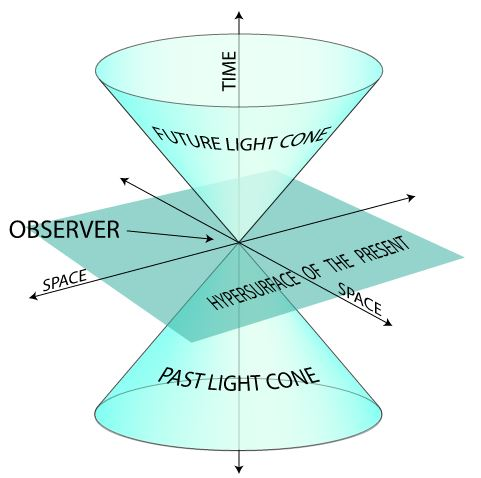
\includegraphics[width=4.2 cm]{pic/space.jpg}
\caption{间隔/时空区域的划分.}
\label{space}
\end{center}
\end{figure}


\subsubsection{惯性变换/洛伦兹~boost}

设坐标系~$\Sigma'$ 与~$\Sigma$ 的三轴分别平行, 前者沿后者~$x$ 轴的负方向以速度~$v$ 运动; 那么, 由光速不变性或由其进一步导致的间隔不变性, 一个事件, 若在~$\Sigma$ 系看来坐标是~$x^\mu=(ct, x, y, z)$, 则在~$\Sigma'$ 系看来其坐标就是
%\begin{equation}
%\left\{
%\begin{array}{l}
%ct'=\frac{ct+\frac{v}{c}x}{\sqrt{1-\frac{v^2}{c^2}}},\\
%x'=\frac{vt+x}{\sqrt{1-\frac{v^2}{c^2}}},\\
%y'=y,\\
%z'=z;
%\end{array}
%\right.
%\end{equation}
\begin{equation}
\left\{
\begin{aligned}
ct'&=\frac{ct+\frac{v}{c}x}{\sqrt{1-\frac{v^2}{c^2}}},\\
x'&=\frac{vt+x}{\sqrt{1-\frac{v^2}{c^2}}},\\
y'&=y,\\
z'&=z;
\end{aligned}
\right.
\end{equation}
上述变换即同一事件在不同惯性系中的变换式, 亦称为洛伦兹变换在~$x$ 方向上的~boost. 我们还可将上述变换用矩阵形式表为
\begin{align}
\left[
\begin{array}{l}
ct'\\x'\\y'\\z'
\end{array}
\right]=
\left[
\begin{array}{cccc}
\gamma&\beta\gamma&0&0\\
\beta\gamma&\gamma&0&0\\
0&0&1&0\\
0&0&0&1
\end{array}
\right]
\left[
\begin{array}{l}
ct\\x\\y\\z
\end{array}
\right];
\end{align}
其中已命
\begin{align}
\gamma=\frac{1}{\sqrt{1-\frac{v^2}{c^2}}},~\beta=\frac{v}{c}.
\end{align}
显然, 有~$\gamma^2-(\beta\gamma)^2=1$.



最后, 我们不难写出洛伦兹惯性变换的矢量表达式:
\begin{gather}
t'=\gamma\left(t+\frac{\bm{r}\cdot\bm{v}}{c^2}\right),\\
\bm{r}'=\bm{r}+(\gamma-1)r_v\bm{v}^0+\gamma t\bm{v}.
\end{gather}

\subsubsection{四维量的协变性与三维量的相对性: 间隔膨胀, 长度收缩, 同时相对}


由洛伦兹变换可见, 某事件的时间间隔, 或某物体的长度/体积, 若在固定于它身上的坐标系--取为~$\Sigma'$--看来是~$\Delta\tau,~l_0$ 或~$V_0$, 称为固有时, 固有长度等, 则在~$\Sigma$ 看来就是
\begin{gather}
\Delta t=\gamma_0\Delta\tau,~l=l_0/\gamma_0,~dV=dV_0/\gamma_0.
\end{gather}
显然, 因为时间, 长度与体积等并不是四维量, 而只是作为四维标量的间隔~$ds^2$ 的一部分, 所以在不同参考系下它们的值将发生变化, 自然是不奇怪的. 事实上, 包括我们稍后要讲到的电磁学, 它们的相对论效应, 就出在我们对作为四维协变量的分量化观察之中.

%上述, 是考察在动系看来, 物体本身为系, 这样子的变化的; 当然, 也可以考察一个长度, 时间, 或体积, 任意两个动系间看起来它们的变化情况, 但, 这意义不大.


%在我中静止的物体, 我看, 与动者看, 我是大的, 动者看是小的.

\subsubsection{狭义相对性原理: 物理规律四维协变}

我们相信, 一切惯性系都应是等价在, 物理规律在何任惯性系中都应被表为相同的形式. 具体操作上讲, 这要求物理规律方程中的出现的每个物理量, 都应是洛伦兹协变量. 这, 称为狭义相对性原理. 它与光速不变事实一起, 就可揭示出关于我们这个世界的很多以前不为人知的事实. 而当然, 此理论的正确性, 也由这些事实的被发现得以确证.


\subsection{力学的洛伦兹协变性; 新发现: 能动关系与质能等价}

力学的以伽利略变换作为时空背景的牛顿表述, 显然不具有洛伦兹不变性. 那么首先, 我们来构造洛伦兹协变的力学规律. 我们定义四维速度:
\begin{align}
u^\mu:=\frac{dx^\mu}{d\tau}=\gamma_0\frac{dx^\mu}{dt}=\gamma_0(c,\bm{u}).
\end{align}
下面我们证明, 此量的确是一个协变的洛伦兹矢量. 我们知道, 对任意空度规空间, 与其中坐标有着相同变换关系的量, 称为矢量. 于是证明~$u^\mu=\gamma_0(c,\bm{u})$ 为洛伦兹矢量, 等价于证明~$c\gamma'_0=\gamma(c\gamma_0+\beta u_x\gamma_0)$ 或~$u'_x\gamma'_0=\gamma(\beta c\gamma_0+u_x\gamma_0)$. 注意其中我们已取~$u^1=\gamma_0 u_x$. 由前述洛伦兹~boost 我们可以直接推得三维速度矢量的变换式为\footnote{由此亦可得出~$\gamma=\gamma_0\gamma'_0(1-\beta_0\beta'_0)$.}
\begin{align}
u'_x=\frac{u_x+v}{1+\frac{u_x v}{c^2}};
\end{align}
而可以发现, 此式与前述待证明的两式是互致的. 于是~$u^\mu$ 是洛伦兹矢量得证. 另外, 两个洛伦兹矢量得到一个洛伦兹标量; 如果四维速度矢量作如上定义的话, 这就是~$\gamma_0^2c^2-\gamma_0^2u^2=c^2$; 而此式的确是成立的. 于是再一次辅证了~$u^\mu$  的洛伦兹矢量性.\footnote{本段分析亦表明, 不像~$(x,y,z)$ 仍是四维协变坐标的三维分量, $\gamma_0 u_x,~\gamma_0 p_x$ 才是四维速度/四维动量的三维分量. 这也就意味着, 我们对牛顿理论中的速度与动量的定义作了改造.%: 在低速三维情况时, 不像坐标仍可精确表为~$(x,y,z)$, 速度与动量等表述为~$\gamma_0 u_x$ 或~$\gamma_0 p_x$ 才是精确的; 只在速度或动量为零, 即物体静止时, 才有~$\gamma_0 p_x=p_x$ 回到牛顿理论中的定义.
}


有了以上之铺垫, 洛伦兹协变的动量四维矢量就可定义为
\begin{align}
p^\mu:=m_0u^\mu=(\gamma_0 m_0c,\gamma_0 m_0\bm{u})=(\frac{\gamma_0 m_0c^2}{c},\bm{p})=(\frac{E}{c},\bm{p})
\end{align}
(由此可看出~$Et-\bm{p}\cdot\bm{r}=p^\mu x_\mu$ 是四维标量); 上式中取~$E=\gamma_0 m_0c^2$ 的原因, 是作泰勒展开可以发现~$\gamma_0 m_0c^2=m_0c^2+\frac{1}{2}m_0v^2+\cdots$. 于是我们发现, 当物体静止时, 仍有~$E_0=m_0c^2$ 的能量, 这称为质能等价; 而~$\frac{E^2}{c^2}-\bm{p}^2=m_0^2c^2$, 即
\begin{align}
E^2=\bm{p}^2c^2+m_0^2c^4,
\end{align}
称为能动关系. 刚才已经知道, 矢量与坐标有着相同变换关系. 所以, 例如对于动量, 假设两系沿~$i$ 轴运动, 我们就有~(已采用自然单位):
\begin{gather}\label{titi}
E'=\gamma(E+\beta p^i),~p'^i=\gamma(\beta E+p^i).
\end{gather}
不难上述第一式, 作为早先发现的~$E=\gamma_0E_0$~或~$E'=\gamma'_0E_0$ 的更一般的推广, 的确是可以给出后二者及其关系的: $\gamma'_0E_0=\gamma(\gamma_0E_0+\beta E_0u_x\gamma_0)\rightarrow\gamma'_0=\gamma(\gamma_0+\beta u_x\gamma_0)$.

最后, 我们把牛顿力学改造洛伦兹协变的版本. 首先我们定义~$F^\mu:=\frac{dp^\mu}{d\tau}$. 考察此四维力的空间分量, 得出~$\bm{F}=\frac{d\bm{p}}{d\tau}$; 其中三维动量的定义与前文是一致的, 即~$\bm{p}=\gamma_0m_0\bm{u}$; 相似地, 四维力的三维空间分量, 相比较牛顿理论中的, 亦是被作了改造的. 考察四维力的零分量, 得出~$F^0=\frac{dp^0}{d\tau}=\frac{1}{c}\frac{dE}{d\tau}=\frac{1}{c}\frac{c^2\bm{p}}{E}\cdot\frac{d\bm{p}}{d\tau}=\frac{\bm{u}\cdot\bm{F}}{c}$; 注意其中~$c^2\bm{p}=E\bm{u}$. 于是最终我们获得~$F^\mu=(\frac{\bm{F}\cdot\bm{u}}{c},\bm{F})$.






\subsection{电磁学的相对论效应, 电动力学的洛伦协协变性}
\subsubsection{光的多普勒效应与光行差的严格公式}
经典的波与动运物体, 就可能出现多普勒效应与~``行差'' 现象; 但光的多普勒效应与光行差现象, 只有使用狭义相对论, 才能给出严格结果. 这些效应, 当然出在我们对四维波矢的分量化观察之中. 下面我们具体考察之.

首先, 不难明确, 相位因子~$\omega t-\bm{k}\cdot\bm{r}$ 应该是洛伦兹标量. 如此, 如下构造四维波矢就是合适的~$k^\mu=(\frac{\omega}{c},\bm{k})$. 由此我们可以得出~$\ frac{\omega'}{c}=\gamma(\frac{\omega}{c}+\beta k_x),~k'_x=\gamma(\beta\frac{\omega}{c}+k_x)$; 若再设~$\bm{k}',~\bm{k}$ 与~$x$ 轴正方向的夹角分别为~$\theta',~\theta$, 即~$k_x=\frac{\omega}{c}\cos\theta,~k'_x=\frac{\omega}{c}\cos\theta'$-- 其中用到了~$\omega=kc$, 则前两式变成
\begin{gather}
\omega'=\omega\gamma\left(1+\frac{v}{c}\cos\theta\right),\tan\theta'=\frac{\sin\theta}{\gamma\left(\cos\theta+\frac{v}{c}\right)};
\end{gather}
此即相对应效应多普勒公式与光行差公式. 进一步地, 我们设光源静止于~$\Sigma'$ 系, $\omega'=\omega_0$ 即光源自己来看的辐射角频律, 于是
\begin{align}
\omega=\frac{\omega_0}{\gamma\left(1+\frac{v}{c}\cos\theta\right)}
\end{align}
即~$\Sigma$ 系中的观测者测出的角频; 其中~$\theta$ 即观测者看到的辐射方向与光源运动方向的夹角. 由此可以看出光的多普勒效应的经典公式的确作为上式的低速近似出现. 另外, 在垂直于光源运动方向的方向上, 相对论公式给出~$\omega=\omega_0\sqrt{1-\frac{v^2}{c^2}}$; 此效应称为横向多普勒效应. 作为比较, 此情况下多普勒效应经典公式仍给出~$\omega=\omega_0$, 即未能预言出应有的现象. 这进一步说明经典理论的不足以及相对论的正确性.










我们将看到, 不同于力学牛顿理论的需要被改造, 电磁学背后的动力学规律, 即电动力学, 或具体地说即麦克斯韦方程组, 是相对论协变的. 接下来我们重点研究之.

\subsubsection{麦克斯韦方程组的四维协变形式}
麦克斯韦方程组的三维矢量式为
\begin{gather}
\nabla\cdot\bm{E}=\frac{\rho}{\epsilon_0},\\
\nabla\times\bm{B}=\mu_0\bm{J}+\mu_0\epsilon_0\frac{\partial\bm{E}}{\partial t},\\
\nabla\cdot\bm{B}=0,\\
\nabla\times\bm{E}=-\frac{\partial\bm{B}}{\partial t};
\end{gather}
其中~$c=\frac{1}{\sqrt{\mu_0\epsilon_0}}$, 是光速. 我们可以引入矢势与标势, 有
\begin{gather}
\bm{B}=\nabla\times\bm{A},~\bm{E}=-\nabla\varphi-\frac{\partial\bm{A}}{\partial t}.
\end{gather}
下面我们要找出麦克斯韦方程组的四维形式. 为此, 将以上两式用分量形式写出, 即~$B^i=\partial_jA^k-\partial_kA^j,~E^i=-\partial_icA^0-c\partial_0A^i$; 其中构造了~$A^\mu=(\frac{\varphi}{c},\bm{A})$, 以及~$\partial_\mu:=\frac{\partial}{\partial x^\mu}=(\partial_0,\partial_i)=(\frac{\partial}{\partial t},\nabla)$. 进一步变形及命令, 可得:
\begin{align}
-B^i&=\partial^jA^k-\partial^kA^j:= F^{jk},\\
-\frac{E^i}{c}&=\partial^0A^i-\partial^iA^0:= F^{0i};
\end{align}
此即意味着场强与势的关系可合写为并列出分量值为:
\begin{align}
F^{\mu\nu}=\partial^\mu A^\nu-\partial^\nu A^\mu=
\left[
\begin{array}{cccc}
0&-E_x/c&-E_y/c&-E_z/c\\
E_x/c&0&-B_z&B_y\\
E_y/c&B_z&0&-B_x\\
E_z/c&-B_y&B_x&0
\end{array}
\right].
\end{align}
其中~$F^{\mu\nu}$ 即由~$\bm{E}$ 与~$\bm{B}$ 构成的电磁场张量. 显然, 上述逆变形式的电磁场张量是反对称的. 我们还可写出电磁场张量的其它形式, 如混合张量
\begin{align}
{F^\mu}_\nu=\partial^\mu A_\nu-\partial^\nu A_\mu=F^{\mu\alpha}g_{\alpha\nu}=
\left[
\begin{array}{cccc}
0&E_x/c&E_y/c&E_z/c\\
E_x/c&0&B_z&-B_y\\
E_y/c&-B_z&0&B_x\\
E_z/c&B_y&-B_x&0
\end{array}
\right].
\end{align}
相应地, 我们可将麦克斯韦方程组分别表为
\begin{gather}
\partial_xF^{x0}+\partial_yF^{y0}+\partial_zF^{z0}=\partial_iF^{i0}=\mu_0 J^0,\\
\partial_jF^{ji}+\partial_kF^{ki}+\partial_0F^{0i}=\partial_jF^{ji}+\partial_0F^{0i}=\mu_0J^i,\\
\partial_iF_{jk}+\partial_jF_{ki}+\partial_kF_{ij}=0,\\
\partial_jF^{k0}+\partial_kF^{0j}-\partial_0F^{jk}=0;
\end{gather}
其中作了构造\footnote{同时~$J^\mu=\rho_0 u^\mu=\rho_0\gamma_0(c,\bm{u})$, 对比知~$\rho=\rho_0\gamma_0$; 这恰好补偿了体积的变化~$dV=dV_0/\gamma_0$, 使总电荷~$Q=\int dV\rho$ 保持为洛伦兹标量. 另外, 可见电荷守恒定律~$\frac{\partial\rho}{\partial t}+\nabla\cdot\bm{J}=\partial_\mu J^\mu=0$ 是洛伦兹不变的.}~$J^\mu=(c\rho,\bm{J})$. 上述方程前两式与后两式可进一步分别合写为
\begin{gather}
\partial_\mu F^{\mu\nu}=\mu_0J^\nu,\\
\partial_\mu F_{\nu\rho}+\partial_\nu F_{\rho\mu}+\partial_\rho F_{\mu\nu}=0;
\end{gather}
此即麦克斯韦方程组的四维协变形式. 由此我们知晓, 电磁学规律天生就是四维协变的.% 另外, 能导出电磁场的拉氏密度是~$\mathcal{L}=\frac{1}{4}F_{\mu\nu}F^{\mu\nu}$.
另外还可读出, 麦氏方程前两式是独立的, 而后两式, 作为~Bianchi 恒等式, 是~$F^{\mu\nu}$ 自然的拓扑性质.

我们知道对任何一个二阶张量都有~$T_{\mu\nu}=\frac{1}{2}(T_{\mu\nu}+T_{\mu\nu})+\frac{1}{2}(T_{\mu\nu}-T_{\mu\nu})\equiv T_{(\mu\nu)}+T_{[\mu\nu]}$, 即任一二阶张量都可由一个对称张量与一个反对称张量构成; 如对电磁场张量我们有~$F_{[\mu\nu]}=F_{\mu\nu}$. 如果我们如下定义一个三阶张量的全反对称张量: $T_{[\rho\mu\nu]}=\frac{1}{6}(T_{\rho\mu\nu}+T_{\mu\nu\rho}+T_{\nu\rho\mu}-T_{\rho\nu\mu}-T_{\nu\mu\rho}-T_{\mu\rho\nu})$, 则可知
\begin{gather}
\partial_{[\rho}F_{\mu\nu]}=\frac{1}{3}(\partial_\mu F_{\nu\rho}+\partial_\nu F_{\rho\mu}+\partial_\rho F_{\mu\nu})=0;
\end{gather}
上式可为麦克斯韦方程第二式的另一写法.

\subsubsection{势的规范冗余, 达朗贝尔方程的四维协变式}

容易推导出电磁势满足
\begin{gather}
\nabla^2\bm{A}-\frac{1}{c^2}\frac{\partial^2\bm{A}}{\partial t^2}-\nabla\left(\nabla\cdot\bm{A}+\frac{1}{c^2}\frac{\partial\varphi}{\partial t}\right)=-\mu_0\bm{J},\\
\nabla^2\varphi+\frac{\partial}{\partial t}\nabla\cdot\bm{A}=-\frac{\rho}{\epsilon_0}
\end{gather}
称为达朗贝尔方程. 由前述势与场强的关系表达式可以看出, 场强在以下两式进行协同变换--称为规范变换--时保持不变:
\begin{gather}
\bm{A}\rightarrow\bm{A}'=\bm{A}+\nabla\gamma,~\varphi\rightarrow\varphi'=\varphi-\frac{\partial\gamma}{\partial t};
\end{gather}
用四维语言叙述上两式合成~$A^\mu\rightarrow A'^\mu=A^\mu-\partial^\mu\gamma$. 也就是说, $(\frac{\varphi}{c},\bm{A})$ 与~$(\frac{\varphi'}{c},\bm{A}')$ 描述的是同一个物理实体. 势的这种规范冗余, 意味着我们可以给它加上条件, 称为规范条件. 常见的有库仑规范~$\nabla\cdot\bm{A}=0$, 与洛伦茨规范~$\nabla\cdot\bm{A}+\frac{1}{c^2}\frac{\partial\varphi}{\partial t}=\partial_\mu A^\mu=0$. 显然洛伦茨规范条件是协变的; 其下势方程化为
\begin{gather}
\nabla^2\bm{A}-\frac{1}{c^2}\frac{\partial^2\bm{A}}{\partial t^2}=-\mu_0\bm{J},~\nabla^2\varphi-\frac{1}{c^2}\frac{\partial^2\varphi}{\partial t^2}=-\frac{\rho}{\epsilon_0};
\end{gather}
上两式可合写为~$\partial^2 A^\mu=-\mu_0 J^\mu$, 显然亦是协变的.

当采取库仑规范时, 有~$\nabla^2\varphi=-\frac{\rho}{\epsilon_0}$. 对于自由场, 就得到~$\varphi=0$. 此式连同库仑规范条件, 称为辐射规范. --有人亦将之称为库仑规范. 在辐射规范下, 势方程就变为~$\partial^2\bm{A}=0$.

辐射规范的两个条件, 将电磁场的自由度由~4 降到了~2; 具体地, 对于平面波, 本规范给出~$\bm{k}\cdot\bm{A}=0$; 也即电磁场只有两个横向分量是自由有的, 没有纵向分量. 这, 与我们熟知的事实是一致的. 但是, 当然, 此规范是不具有洛伦兹协变性的. 如上所见, 洛伦茨规范倒是洛伦兹协变的, 但却不能消除所有非物理自由度.




\subsubsection{麦克斯韦方程组用微分形式表达}

电磁势用微分形式写出就是~$A=A_\mu dx^\mu$, 是一个~1-形式; 于是可以看出, 由其得出的如下~2-形式:
\begin{align}
F=dA=\partial_{[\mu}A_{\nu]}dx^\mu\wedge dx^\nu=\frac{1}{2}(\partial_\mu A_\nu-\partial_\nu A_\mu)dx^\mu\wedge dx^\nu=\frac{1}{2}F_{\mu\nu}dx^\mu\wedge dx^\nu,
\end{align}
即电磁场强; $F_{\mu\nu}$ 即电磁场张量. 我们知道外微分算符~$d$ 总有~$d^2=0$, 此即给出麦克方程第二式~$\partial_{[\rho}F_{\mu\nu]}=0$. 具体地,
\begin{gather}
dF=d^2A=\frac{1}{2}\partial_{[\rho}F_{\mu\nu]}dx^\rho\wedge dx^\mu\wedge dx^\nu=0.
\end{gather}
利用~Hodge 星算符\footnote{
利用此算符的定义~$\star(dx^{i_1}\wedge\cdots\wedge dx^{i_p})=\frac{1}{q!}{\epsilon_{j_1\cdots j_q}}^{i_1\cdots i_p}dx^{j_1}\wedge\cdots\wedge dx^{j_q}$, 可求得
\begin{gather}
\star dt=dx^i\wedge dx^j\wedge dx^k,~\star dx^i=dt\wedge dx^j\wedge dx^k;\\
\star (dt\wedge dx^i)=-dx^j\wedge dx^k,~\star(dx^i\wedge dx^j)=dt\wedge dx^k.
\end{gather}
%\begin{gather}
%\star dt=dx\wedge dy\wedge dz,~\star dx=dt\wedge dy\wedge dz,~\star dy=dt\wedge dz\wedge dx,~\star dz=dt\wedge dx\wedge dy;\\
%\star (dt\wedge dx)=-dy\wedge dz,~\star(dt\wedge dy)=-dz\wedge dx,~\star(dt\wedge dz)=-dx\wedge dy,\\
%\star(dx\wedge dy)=dt\wedge dz,~\star(dz\wedge dx)=dt\wedge dy,~\star(dy\wedge dz)=dt\wedge dx.
%\end{gather}
}~$\star$, 可求出
\begin{align}
d\star F=&d\star\left(\frac{1}{2}F_{\mu\nu}dx^\mu\wedge dx^\nu\right)\nonumber\\
=&d\star\left(F_{0i}dx^0\wedge dx^i+\frac{1}{2}F_{ij}dx^i\wedge dx^j\right)\nonumber\\% 这是总项
=&d\left(F_{i0}dx^j\wedge dx^k+F_{ij}dx^0\wedge dx^k\right)\nonumber\\%这里变成了单项, 需要循环相加
=&\partial_iF_{i0}dx^i\wedge dx^j\wedge dx^k+\partial_iF_{ij}dx^i\wedge dx^0\wedge dx^k\nonumber\\
=&-\mu_0\star J_0dx^0+\mu_0\star J_jdx^j\nonumber\\
=&-\mu_0\star J;
\end{align}
其中~$J=J_\mu dx^\mu$ 为一个~1-形式. 显然, 上述式子即麦氏方程前两式之合写.
%\begin{align}
%d\star F=&d\star\left(\frac{1}{2}F_{\mu\nu}dx^\mu dx^\nu\right)\\
%=&d\star(F_{01}dx^0\wedge dx+F_{02}dx^0\wedge dy+F_{03}dx^0\wedge dz\\
%&+F_{12}dx\wedge dy+F_{31}dz\wedge dx+F_{23}dy\wedge dz)\\
%=&d(-F_{01}dy\wedge dz-F_{02}dz\wedge dx-F_{03}dx\wedge dy\\
%&+F_{12}dt\wedge dz+F_{31}dt\wedge dy+F_{23}dt\wedge dx)\\
%=&-\mu_0\star J.
%\end{align}



\subsection{洛伦兹群表示论}%: 场的性质~(标量/矢量/旋量) 与粒子自旋的关系--Wigner 定理; 旋量, 狄拉克方程的严格导出, 物理规律的~$CPT$ 离散变换性质}

闵氏时空的对称群, 是洛伦兹/庞加莱群; 前者的几何性质由后者精确体现. 特别地, 对洛伦兹群表示理论的研究, 将使我们看到作为群的表示基的场函数的自旋的出现, 以及后者与场的性质的对应关系; 还可使我们发现旋量, 并严格推导出旋量满足的狄拉克方程. 我们还将仔细探讨物理规律在~$CPT$ 三个离散操作之下的变换性质.

\subsubsection{正当正时的六个洛伦兹变换的具体形式}
我们已经知道, 在洛伦兹变换中有~$\gamma^2-(\beta\gamma)^2=1$; 因为双曲三角函数\footnote{双曲余弦, 双曲正弦的定义及关系为
\begin{align}
\cosh x=\frac{e^x+e^{-x}}{2},~\sinh=\frac{e^x-e^{-x}}{2};~\cosh^2x-\sinh^2x=1.
\end{align}}恰有此性质, 所以若令
\begin{align}
\gamma=\cosh\zeta,~\beta\gamma=\sinh\zeta,
\end{align}
--其中~$\zeta$ 称为~rapidity, --则~$x$ 方向上的洛伦兹~boost 就进一步可表为\footnote{我们将用到三角函数或双曲三角函数与指数函数的关系等知识. 现摘其相关, 简列如下. 据泰勒展开: $f(x)=\sum_{n=0}^\infty\frac{f^{(n)}(x_0)}{n!}(x-x_0)^n$, 可得
\begin{gather}
\cos x=1-\frac{1}{2}x^2+\frac{1}{4!}x^4-\cdots,~\sin x=x-\frac{1}{3!}x^3+\frac{1}{5!}x^5-\cdots,\\
\cosh x=1+\frac{1}{2}x^2+\frac{1}{4!}x^4+\cdots,~\sinh x=x+\frac{1}{3!}x^3+\frac{1}{5!}x^5+\cdots,\\
e^x=1+x+\frac{1}{2}x^2+\frac{1}{3!}x^3+\cdots;%~e^{ix}=\cos x+i\sin x,~e^x=\cosh x+\sinh x;\\
\end{gather}
于是可得
\begin{gather}
\left[
\begin{array}{cc}
\cos\theta&\sin\theta\\
-\sin\theta&\cos\theta
\end{array}
\right]=
\exp
\left[
\begin{array}{cc}
0&\theta\\
-\theta&0
\end{array}
\right],~
\left[
\begin{array}{cc}
\cosh\zeta&\sinh\zeta\\
\sinh\zeta&\cosh\zeta
\end{array}
\right]=
\exp
\left[
\begin{array}{cc}
0&\zeta\\
\zeta&0
\end{array}
\right].
\end{gather}
}
\begin{align}
\left[
\begin{array}{l}
ct'\\x'\\y'\\z'
\end{array}
\right]=
\left[
\begin{array}{cccc}
\cosh\zeta&\sinh\zeta&0&0\\
\sinh\zeta&\cosh\zeta&0&0\\
0&0&1&0\\
0&0&0&1
\end{array}
\right]
\left[
\begin{array}{l}
ct\\x\\y\\z
\end{array}
\right]
=\exp\left[
\begin{array}{cccc}
0&\zeta&0&0\\
\zeta&0&0&0\\
0&0&0&0\\
0&0&0&0
\end{array}
\right]
\left[
\begin{array}{l}
ct\\x\\y\\z
\end{array}
\right].
\end{align}
于是一个一般的洛伦兹~boost 就是
\begin{align}
\left[
\begin{array}{l}
ct'\\x'\\y'\\z'
\end{array}
\right]
=\exp\left[
\begin{array}{cccc}
0&\zeta_x&\zeta_y&\zeta_z\\
\zeta_x&0&0&0\\
\zeta_y&0&0&0\\
\zeta_z&0&0&0
\end{array}
\right]
\left[
\begin{array}{l}
ct\\x\\y\\z
\end{array}
\right].
\end{align}
不难知晓, 连续操作部分的洛伦兹变换, 应包含空间方向上的三个~boost 以及三个旋转这六个操作. Boost 部分业已写出, 下面我们研究旋转部分. 坐标系绕~$z$ 轴正方向作逆时针旋转, 同一个事件在两系中的变换操作为
\begin{align}
\left[
\begin{array}{l}
ct'\\x'\\y'\\z'
\end{array}
\right]=
\left[
\begin{array}{cccc}
1&0&0&0\\
0&\cos\theta&\sin\theta&0\\
0&-\sin\theta&\cos\theta&0\\
0&0&0&1
\end{array}
\right]
\left[
\begin{array}{l}
ct\\x\\y\\z
\end{array}
\right]
=\exp\left[
\begin{array}{cccc}
0&0&0&0\\
0&0&\theta&0\\
0&-\theta&0&0\\
0&0&0&0
\end{array}
\right]
\left[
\begin{array}{l}
ct\\x\\y\\z
\end{array}
\right].
\end{align}
至此, 三个方向上的~boost 与旋转操作下, 事件在前后坐标系中的关系为
\begin{align}
\left[
\begin{array}{l}
ct'\\x'\\y'\\z'
\end{array}
\right]
=\exp\left[
\begin{array}{cccc}
0&\zeta_x&\zeta_y&\zeta_z\\
\zeta_x&0&\theta_z&-\theta_y\\
\zeta_y&-\theta_z&0&\theta_x\\
\zeta_z&\theta_y&-\theta_x&0
\end{array}
\right]
\left[
\begin{array}{l}
ct\\x\\y\\z
\end{array}
\right];
\end{align}
这个结果, 是相当之优美的. 一般地, 我们可将上述变换记为\footnote{
为作储备, 我们写出张量与度规运算的以下一些基础:
\begin{gather}
\omega^{\mu\nu}={\omega^\mu}_\alpha g^{\alpha\nu}=g^{\mu\alpha}{\omega_\alpha}^\nu,~\omega_{\mu\nu}={\omega_\mu}^\alpha g_{\alpha\nu}=g_{\mu\alpha}{\omega^\alpha}_\nu,\\
{\omega^\mu}_\nu=\omega^{\mu\alpha}g_{\alpha\nu}=g^{\mu\alpha}\omega_{\alpha\nu},~{\omega_\mu}^\nu=\omega_{\mu\alpha}g^{\alpha\nu}
=g_{\mu\alpha}\omega^{\alpha\nu};\\
x'^\mu={\Lambda^\mu}_\nu x^\nu,~x'_\mu=\Lambda_{\mu\nu}x^\nu,~x'^\mu=\Lambda^{\mu\nu}x_\nu,~x'_\mu={\Lambda_\mu}^\nu x_\nu.
\end{gather}
规则可以简记为: 度规从后面作用时, 后三列变号; 从前面作用时, 后三行变号.}
\begin{align}
x'^\mu={\Lambda^\mu}_\nu x^\nu,
\end{align}
其中~$[{\Lambda^\mu}_\nu]=\exp[{\omega^\mu}_\nu]$.
%
%蕴含在~${\Lambda^\mu}_\nu$ 或~${\omega^\mu}_\nu$ 中的六个连续操作, 所刻画的几何, 称为闵氏几何, 表征了~(不考虑引力时) 我们所存在的这个时空的真实面貌. 另外
%
可以看出, 对洛伦兹变换的六个操作~(或由它们组合成的任意操作) 皆有~$\det[{\Lambda^\mu}_\nu]=+1,~{\Lambda^0}_0\geq1$, 我们称这样的变换是正当正时的. 另外它们还有如下一些关系: ${(\Lambda^{-1})^\mu}_\nu={\Lambda_\nu}^\mu,~(\Lambda^{-1})^{\mu\nu}=\Lambda^{\nu\mu},~{(\Lambda\Lambda^{-1})^\mu}_\nu=
{\Lambda^\mu}_\alpha{(\Lambda^{-1})^\alpha}_\nu={\Lambda^\mu}_\alpha{\Lambda_\nu}^\alpha={\delta^\mu}_\nu,~[{\Lambda^\mu}_\alpha{\Lambda_\nu}^\alpha]=I_{4\times4}$.
%
能何持事件间隔不变的操作, 除了以上六个连续操作外, 还有宇称变换与时间反演两个离散操作. 物理规律在它们之下的变换行为, 我们将在本节末研究.


现在我们对洛伦兹变换矩阵进行分解, 以获取对其之进一步认识. 若我们命
\begin{gather}
L({\omega^\mu}_\nu)=-i\frac{\partial D({\omega^\mu}_\nu)}{\partial{\omega_\mu}^\nu}\Big|_{{\omega_\mu}^\nu=0},
\end{gather}
--由此可容易写下~$L({\omega^\mu}_\nu)$ 的矩阵形式, 它们可统一表为
\begin{gather}
({L^\mu}_\nu)_{\alpha\beta}=-i(g^{\mu\alpha}g^{\nu\beta}-{g^\mu}_\beta{g^\nu}_\alpha)=i(g^{\mu\alpha}\delta^{\nu\beta}-\delta^{\mu\beta}g^{\nu\alpha}),
\end{gather}
--则我们可将洛伦兹变换写为:
\begin{gather}
[{\Lambda^\mu}_\nu]=\exp[{\omega^\mu}_\nu]=\exp\left(\frac{i}{2}{\omega_\mu}^\nu L({\omega^\mu}_\nu)\right).
\end{gather}
只要作与前一式相应的命令, 我们还可写出相应的~$[\Lambda_{\mu\nu}]=\exp\left(\frac{i}{2}\omega^{\mu\nu} L(\omega_{\mu\nu})\right)$ 等其它其形式; 当然, 此时角动量矩阵亦将变成~$(L^{\mu\nu})_{\alpha\beta}=-i(g^{\mu\alpha}g^{\nu\beta}-g^{\mu\beta}g^{\nu\alpha})=i(g^{\mu\alpha}\delta^{\nu\beta}-g^{\mu\beta}\delta^{\nu\alpha})$ 等形式. 简单分析可知, 我们有~$L(\omega_{\mu\nu})=L(\omega^{\mu\nu}),~L({\omega^\mu}_\nu)=L({\omega_\mu}^\nu)$.

我们作以下的读取与命令\footnote{对于其它形式, 我们同样可作相应的读取与命令, 如~$\omega_{0i}=\zeta^i,~\omega_{ij}=-\theta^k,~L^{0i}=K^i,~L^{ij}=-J^k$ 等.}:
\begin{gather}
{\omega_j}^k=\theta^i,~{\omega_0}^i=-\zeta^i;~L({\omega^j}_k)=J^i,~L({\omega^0}_i)=-K^i=-i\left[\begin{array}{cc}0&-1\\-1&0\end{array}\right],
\end{gather}
则洛伦兹变换就可写为
\begin{gather}
[{\Lambda^\mu}_\nu]=e^{i(\zeta^iK^i+\theta^iJ^i)}=e^{i(\bm{\zeta}\cdot\bm{K}+\bm{\theta}\cdot\bm{J})}.
\end{gather}
对于洛伦兹变换的其它形式, 如~$[\Lambda^{\mu\nu}]$, 我们仍能给出上述结果, 不过须注意其中矩阵~$K^i,~J^i$ 的形式有相应的不同.



\subsubsection{洛伦兹群的一般李群分析, 场的自旋的出现及其与场性质~(标/矢/旋等) 之间的关系--Wigner 定理}

%群元, 转动角, 角动量/李代数及其分解组合, SO$^+$(3,1)$\sim$SU(2)$\otimes$SU(2), 标/矢/旋等表示与粒子自旋的关系--Wigner 定理}

\paragraph{群元, 转动角}
~

在不用知晓~${\Lambda^\mu}_\nu$ 的具体形式的情况下, 仅通过~$x'^\mu={\Lambda^\mu}_\nu x^\nu$ 以及间隔不变性, 再结合群论的一些知识, 我们就可得到一些有用的信息. 下面我们进行之. 一般地, 我们知道, 物理规律应在十二个操作下保持不变; 这十二个操作分别是空间上的三个~boost 与三个旋转, 时空上的四个平移--这些都是连续操作, 以及时间反演与宇称~(空间反演) 两种离散操作. 其中, 我们将连续操作写为
\begin{gather}
x'^\mu={\Lambda^\mu}_\nu x^\nu+\xi^\mu;
\end{gather}
这样的操作形成的群称为庞加莱群. 下面我们先不考虑时空平移操作, 而只考虑操作~${\Lambda^\mu}_\nu$. 我们已经知道, 上述变换的要求, 是保持间隔不变: $g_{\mu\nu}x'^\mu x'^\nu=g_{\mu\nu}{\Lambda^\mu}_\alpha x^\alpha{\Lambda^\nu}_\beta x^\beta=g_{\alpha\beta}x^\alpha x^\beta$; 亦即间隔不变的等价表述就是:
\begin{gather}\label{interval}
g_{\alpha\beta}=g_{\mu\nu}{\Lambda^\mu}_\alpha {\Lambda^\nu}_\beta.
\end{gather}
设我们现在另有一转动~$\Lambda'$, 同样满足上述结构, 即有~$g_{\alpha\beta}=g_{kt}{\Lambda'^k}_\alpha{\Lambda'^t}_\beta$; 则可发现~$g_{\mu\nu}=g_{kt}{(\Lambda'\Lambda)^k}_\mu{(\Lambda'\Lambda)^t}_\nu$. 也就是说, 满足式~(\ref{interval}) 的变换, 成形一个群; 我们称此群为~O(3,1) 群. 进一步分析可知, $\det[{\Lambda^\mu}_\nu]=\pm1,~{\Lambda^0}_0\geq1~or~\leq-1$; 我们称~$\det[{\Lambda^\mu}_\nu]=+1$ 的情况为正当的, ${\Lambda^0}_0\geq1$ 的情况为正时的. 正当正时的操作构成的子群, 记为~SO$^+$(3,1). 我们常说的兹伦兹群, 一般即指~SO$^+$(3,1) 群.


洛伦兹变换的无穷小如下
\begin{align}
{\Lambda^\mu}_\nu={\delta^\mu}_\nu+{\omega^\mu}_\nu;
\end{align}
也就是说, 当我们作一个无穷小洛伦兹变换时, 可以写出~$x'^\mu=({\delta^\mu}_\nu+{\omega^\mu}_\nu)x^\nu=x^\mu+{\omega^\mu}_\nu x^\nu$, 或~$\delta x^\mu={\omega^\mu}_\nu x^\nu$. --将上式代入前述间隔不变的表达式, 有~$g_{\alpha\beta}=g_{\mu\nu}({\delta^\mu}_\alpha+{\omega^\mu}_\alpha)({\delta^\nu}_\beta+{\omega^\nu}_\beta)=g_{\alpha\beta}+\omega_{\alpha\beta}+\omega_{\beta\alpha}+O(\omega^2)$. 也就是说, 间隔不变性加在洛伦兹无穷小上的要求是后者具有下述结构
\begin{align}
\omega_{\mu\nu}=-\omega_{\nu\mu},
\end{align}
即洛伦兹无穷小必是反对称的. 数学上我们知, 实反对称四维方程的空间是~6 维的; 于是我们知道洛伦兹群是六维的, 即有六个生成元. 本小节至此对洛伦兹变换的一般分析, 与前一小节我们已获知的洛伦兹变换的具体形式, 是完全一致的.




\paragraph{角动量, 一般函数上的洛伦兹操作~$U(\Lambda)$}
~




下面, 我们继续按李群的一般手续语言说话. 考虑到与前文的一致性, 作以下的命令是合适的\footnote{三维情况时此命令退化为~$L^k={L^i}_j=-i(x^i\partial_j-x^j\partial_i)$, 这与我们的通常的做法是相符的.}:
\begin{align}
{L^\mu}_\nu=-i(x^\mu\partial_\nu-x_\nu\partial^\mu);
\end{align}
相似地, 我们也可写出其它的形式, 如~$L^{\mu\nu}=-i(x^\mu\partial^\nu-x^\nu\partial^\mu)$. 由此, 例如按标量在转动下的变换行为~$U(\Lambda)\phi(x)=\phi(\Lambda^{-1}x)$ 并结合上一小节得到的转动矩阵的具体形式, 我们就可得到\footnote{以三维空间为例, 一般地, $P_{R}f(\bm{r})=f(R^{-1}\bm{r})$; 由此即可求得~$P_R$.}:
\begin{align}
U([\Lambda^{\mu\nu}])=\exp\left(\frac{i}{2}\omega_{\mu\nu}L^{\mu\nu}\right),
\end{align}
以及诸如~$U([{\Lambda^\mu}_\nu])=\exp\left(\frac{i}{2}{\omega_\mu}^\nu{L^\mu}_\nu\right)$ 等其它形式. ($L^{\mu\nu}$ 可待矩阵化, $\omega_{\mu\nu}$ 就是一个个分量, 而不是矩阵.) 此是尚是作用在函数空间上的洛伦兹解析操作; 也就是说, 上式中~$L^{\mu\nu}$ 是微分算符, 区别于上一小节中的~$L(\omega^{\mu\nu})$ 是矩阵.

前文业已言明, 或由计算过程我们可以发现, $U(\Lambda)$ 是函数或坐标系经过洛伦兹转动后, 新老函数间的关系, 具体地, 即\footnote{可以与三维空间情况作一比较体会. 在三维空间中, 一般地, $P_R$ 或~$R$ 的矩阵表示由下式拿出~$P_Rf^a(\bm{r})=\sum_bD(R)^a_bf^b(\bm{r})$.}
\begin{gather}
\psi^\alpha(x)\rightarrow\psi'^\alpha(x)=U(\Lambda)\psi^\alpha(x)={M(\Lambda)^\alpha}_\beta\psi^\beta(\Lambda^{-1}x).
\end{gather}
其中, 我们称~${M(\Lambda)^\alpha}_\beta$ 即~$\Lambda$ 或~$U(\Lambda)$ 以~$\psi^\alpha(x)$ 为表示基的表示矩阵. 具体地, 若\footnote{在洛伦兹坐标系变换下, 不考虑坐标点, 标量与矢量的变换行为则分别是~$\phi=1\cdot\phi,~A^\mu={\Lambda^\mu}_\nu A^\nu$. 另, $\phi$ 读作老函数, $\phi'$ 读作新函数.}
\begin{gather}
\phi(x)\rightarrow\phi'(x)=U(\Lambda)\phi(x)=I\cdot\phi(\Lambda^{-1}x),\\
A^\mu(x)\rightarrow A'^\mu(x)=U(\Lambda)A^\mu(x)={\Lambda^\mu}_\nu A^\nu(\Lambda^{-1}x),
\end{gather}
则表示基~$\psi(x)$ 与~$A^\mu(x)$ 分别就是标量与矢量, 相应的表示~$I,~{\Lambda^\mu}_\nu$ 就称为~$\Lambda$ 或~$U(\Lambda)$ 的标量表示与矢量表示. 须要注意, 当场被算符化以后, 以标量场为例, 洛伦兹变换对场算符的作用将变成~$U(\Lambda)\phi(x)U^{-1}(\Lambda)$ 这样的形式.



\paragraph{角动量/李代数及其分解组合, SO$^+$(3,1)$\sim$SU(2)$\otimes$SU(2), 洛伦兹群~($\Lambda$ 或~$U(\Lambda)$) 的矩阵表示, 场的自旋的出现及其与场性质~(标/矢/旋等) 之间的关系--Wigner 定理}
~

群表示论中, 我们要做的最重要的事之一, 就是找到~$U(\Lambda)$ 或~$\Lambda$ 的不同矩阵表示. 不同的表示基函数, 就是洛伦兹标量, 矢量与旋量等; 相应的表示就称为标量表示, 矢量表示与旋量表示等. 而同时可以发现, 与标量函数, 矢量函数与旋量函数, 还将分别带有零自旋~0, 自旋~1 以及自旋~1/2. 在稍后的量子场论中我们知道, 粒子将由洛伦兹协变的场描述; 于是前述场的自旋, 就是相应的粒子的自旋. 洛伦兹群的带有某个自旋角动量的场, 对应于物理世界中具有相应角动量的某种粒子, 这, 称为~Wigner 定理. 下面我们就来按手续进行.





利用~$p^\mu=i\partial^\mu,~[x^\mu,p^\nu]=-ig^{\mu\nu}$, 我们容易算出本群的李代数:
\begin{align}
[L^{\mu\nu},L^{\rho\sigma}]=ig^{\mu\sigma}L^{\rho\nu}+ig^{\nu\sigma}L^{\mu\rho}-ig^{\nu\rho}L^{\mu\sigma}-ig^{\mu\rho}L^{\sigma\nu}.
\end{align}
我们知道, 每一组满足上述李代数的矩阵, 即构成~$U(\Lambda)$ 或~$\Lambda$ 的一个表示. 我们将~$L^{\mu\nu}$ 作如下分解, 即分别考察其时间部分与空间部分:
\begin{align}
K^i=L^{0i},~J^i=-L^{jk},
\end{align}
--此时同样我们可写出作为解析表达式的~$U(\Lambda)=e^{i(\bm{\zeta}\cdot\bm{K}+\bm{\theta}\cdot\bm{J})}$ 系列式子, --则将其代入前述李代数一般式立即可得出
\begin{align}
[J^i,J^j]=iJ^k,~[K^i,K^j]=-iJ^k,~[K^i,L^j]=iK^k.
\end{align}
由此可见, $K^i$ 操作并不封闭, 也就是说, 洛伦兹~boost 并不能形成一个子群. 而若我们将操作作下述组合:
\begin{align}
A^i=\frac{J^i+iK^i}{2},~B^i=\frac{J^i-iK^i}{2},
\end{align}
则立可发现
\begin{align}
[A^i,A^j]=iA^k,~[B^i,B^j]=iB^k,~[A^i,B^j]=0;
\end{align}
也就是说, SO$^+$(3,1)$\sim$SU(2)$\otimes$SU(2). 由此, 按此两二维幺模幺正群的本征值, 如记作~$A,B$, 我们即可找出洛伦兹群的各矩阵表示, 如可标记为~$(A,B)$; 且如前文已言明, 我们并可认清特定自旋与场的标/矢/旋之间的关系.


1, $(0,0)$ 表示. 此时~$L^{\mu\nu}=0$, 故有
\begin{align}
M(U(\Lambda))=M(\Lambda)\equiv\Lambda_0=I.
\end{align}
此矩阵表示对应的粒子的自旋为零, 该种粒子用标量场来描述. 这是洛伦兹群的平庸表示.

2, $(\frac{1}{2},\frac{1}{2})$ 表示. 此时~$J^i=1, K^i=0,~(L^{\mu\nu})_{\alpha\beta}=-i(g^{\mu\alpha}g^{\nu\beta}-g^{\mu\beta}g^{\nu\alpha})=i(g^{\mu\alpha}\delta^{\nu\beta}-g^{\mu\beta}\delta^{\nu\alpha})$, 故有
\begin{align}
~\Lambda_{1}=[\Lambda^{\mu\nu}].
\end{align}
也就是说, 此表示对应的的粒子的自旋为~1, 该种粒子用矢量场来描述. 这是洛伦兹群的基本表示.

3, $(0,\frac{1}{2})$ 表示. 此时\footnote{泡利矩阵的性质: $\bm{s}=\frac{\hbar}{2}\bm{\sigma},~\sigma^{i\dag}=\sigma^i,~\{\sigma^i,\sigma^j\}=2\delta_{ij}$ (中含~$(\sigma^i)^2=1$),~$[\sigma^i,\sigma^j]=2i\sigma^k$; 在~$\sigma^3$ 表象中, 有
\begin{align}
\sigma^1=\left[\begin{array}{cc}0&1\\1&0\end{array}\right],~
\sigma^2=\left[\begin{array}{cc}0&-i\\i&0\end{array}\right],~
\sigma^1=\left[\begin{array}{cc}1&0\\0&-1\end{array}\right].
\end{align}
}~$J^i=\frac{1}{2}\sigma^i,~K^i=i\frac{\sigma^i}{2}$, 于是
\begin{align}
\Lambda_{(0,\frac{1}{2})}=\exp\left(-\frac{1}{2}\sigma^i\zeta^i+\frac{i}{2}\sigma^i\theta^i\right).
\end{align}
对于自旋为半奇数的粒子, 这里以自旋~$1/2$ 为例, 若体系在空间转过一周, $U(\Lambda)\psi_L=e^{i\pi}\psi_L=-\psi_L$, 即此时体系并不复原, 而是相差一个负号. 我们称这样的体系的旋量体系, 描述之的波函数, 称为旋量波函数. 因为后面可知的原因, 我们称此表示的表示基函数为左旋外尔旋量.


4, $(\frac{1}{2},0)$ 表示. 此时~$J^i=\frac{1}{2}\sigma^i,~K^i=-i\frac{\sigma^i}{2}$, 故有
\begin{align}
\Lambda_{(\frac{1}{2},0)}=\exp\left(\frac{1}{2}\sigma^i\zeta^i+\frac{i}{2}\sigma^i\theta^i\right).
\end{align}
与前一个表示类似, 我们称此表示为右旋外尔旋量表示, 亦描述某种具有~$1/2$ 自旋的粒子. 别外可以看出, 本粒子与上一种粒子, 对洛伦兹空间转动的反应是相同的, 而对~boost 的反应, 在相位上差一个负号.


\subsubsection{狄拉克方程与外尔方程的严格导出, 螺旋, $\gamma$ 矩阵, 狄拉克表示}

若左右旋外尔粒子具有质量, 则我们就可使自己位于与它们静止的参考系中; 而这时对于我们而言, 这两种粒子将不可分辨. 事实上, 当获得质量后, 左右旋外尔费米子将变成同一种粒子, 称为狄拉克费米子. 下面, 我们就来具体研究这件事, 并导出狄拉克费米子的运动方程, 或即狄拉克旋量满足的方程.
\begin{align}
\psi_L^p=&\exp\left(-\frac{1}{2}\bm{\sigma}\cdot\bm{\zeta}\right)\psi_L^0=\left(\cosh\frac{\zeta}{2}-\bm{\sigma}\cdot\bm{p}^0\sinh\frac{\zeta}{2}\right)\psi_L^0\nonumber\\
=&\left(\sqrt{\frac{\gamma+1}{2}}-\bm{\sigma}\cdot\bm{p}^0\sqrt{\frac{\gamma-1}{2}}\right)\psi_L^0=\frac{E+m-\bm{\sigma}\cdot\bm{p}}{\sqrt{2m(E+m)}}\psi_L^0;
\end{align}
上述推导中用到了双曲三角函数的一些性质, 以及粒子的相对论关系~$E=\gamma m,~|\bm{p}|=\sqrt{E^2-m^2}$. 其中~$\bm{\sigma}\cdot\bm{p}^0$ 描述粒子自旋在动量方向上的投影, 称为螺旋. 同样可推得
\begin{align}
\psi_R^p=&\exp\left(\frac{1}{2}\bm{\sigma}\cdot\bm{\zeta}\right)\psi_R^0=\frac{E+m+\bm{\sigma}\cdot\bm{p}}{\sqrt{2m(E+m)}}\psi_R^0.
\end{align}
粒子在静止时不可分辨, 从而有静止条件~$\psi_L^0=\psi_R^0$; 于是我们可得
\begin{align}
\frac{\psi_L}{\psi_R}=\frac{E+m-\bm{\sigma}\cdot\bm{p}}{E+m+\bm{\sigma}\cdot\bm{p}}=\frac{E-\bm{\sigma}\cdot\bm{p}}{m},~\frac{\psi_R}{\psi_L}=\frac{E+\bm{\sigma}\cdot\bm{p}}{m};
\end{align}
其中用到了~$E^2=(\bm{\sigma}\cdot\bm{p})^2+m^2$. 采用矩阵形式, 上式即可被表为
\begin{align}
\left[\begin{array}{cc}
-m&E-\bm{\sigma}\cdot\bm{p}\\
E+\bm{\sigma}\cdot\bm{p}&-m
\end{array}\right]
\left[\begin{array}{c}\psi_L\\\psi_R\end{array}\right]=
\left[\begin{array}{cc}
-m&\sigma^\mu p_\mu\\
\bar{\sigma}^\mu p_\mu&-m
\end{array}\right]
\left[\begin{array}{c}\psi_L\\\psi_R\end{array}\right]
=0;
\end{align}
其中我们作了命令~$\sigma^\mu=(1,\sigma^i),~\bar{\sigma}^\mu=(1,-\sigma^i)$. --由此亦知~$\bar{\sigma}^\mu p_\mu\sigma^\mu p_\mu=m^2$. 若我们再令\footnote{可知~$\gamma$ 矩阵有性质~$\gamma^{0\dag}=\gamma^0,~\gamma^{i\dag}=-\gamma^i;~\{\gamma^\mu,\gamma^\nu\}=2g^{\mu\nu}$~(中含~$(\gamma^\mu)^2=g^{\mu\mu}$); 当~$\mu\neq\nu$ 时~$[\gamma^\mu,\gamma^\nu]=2\gamma^\mu\gamma^\nu$. 此代数称为~Clifford 代数.}
\begin{align}
\gamma^\mu=
\left[\begin{array}{cc}
0&\sigma^\mu\\
\bar{\sigma}^\mu&0
\end{array}\right]:~
\gamma^0=
\left[\begin{array}{cc}
0&1\\
1&0
\end{array}\right],~
\gamma^i=
\left[\begin{array}{cc}
0&\sigma^i\\
-\sigma^i&0
\end{array}\right],
\end{align}
则我们可将前述式子表为
\begin{align}
\gamma^0=
(\gamma^0p_0+\gamma^ip_i-m)\psi=(\gamma^\mu p_\mu-m)\psi=0;
\end{align}
上式中~$\psi\equiv\left[\begin{array}{c}\psi_L\\\psi_R\end{array}\right]$ 称为狄拉克旋量 此方程即称为狄拉克方程. 注意从数学上讲, 能动关系~$p^2=m^2$ 可分为两个式子: $\gamma^\mu p_\mu=m,~\gamma^\mu p_\mu=-m$, 或~$(\gamma^\nu p_\nu+m)(\gamma^\mu p_\mu-m)=\gamma^\mu\gamma^\nu p_\mu p_\nu-m^2=p^2-m^2=0$.

当粒子无质量, 可见狄拉克方程退化为分别描述左右外尔旋量的两个方程:
\begin{align}
\bar{\sigma}^\mu p_\mu\psi_L=(E+\bm{\sigma}\cdot\bm{p})\psi_L=0,~\sigma^\mu p_\mu\psi_R=(E-\bm{\sigma}\cdot\bm{p})\psi_R=0;
\end{align}
称为外尔方程. 对于无质量粒子, $E=|\bm{p}|$, 于是可得
\begin{align}
\frac{\bm{\sigma}\cdot\bm{p}}{|\bm{p}|}\psi_L=\bm{\sigma}\cdot\bm{p}^0\psi_L=-\psi_L,~\frac{\bm{\sigma}\cdot\bm{p}}{|\bm{p}|}\psi_R=\bm{\sigma}\cdot\bm{p}^0\psi_R=+\psi_R;
\end{align}
由此可知左手外尔旋量的螺旋为~$-1$, 右手的为~+1.


现在我们来找出狄拉克旋量表示的表示矩阵. 我们令~$S^{\mu\nu}=\frac{i}{4}[\gamma^\mu,\gamma^\nu]$; 不难验证此矩阵符合前述洛伦兹群的李代数, 所以它构成洛伦兹群的一个表示:
\begin{align}
\Lambda_{\frac{1}{2}}=\exp\left(\frac{i}{2}\omega_{\mu\nu}S^{\mu\nu}\right).
\end{align}
由以后的具体知识可以确定, 上式即洛伦兹群的狄拉克旋量表示. 进一步, 容易算得
\begin{align}
S^{0i}=-\frac{i}{2}\left[\begin{array}{cc}\sigma^i&0\\0&-\sigma^i\end{array}\right],~S^{ij}=\frac{1}{2}\left[\begin{array}{cc}\sigma^k&0\\0&\sigma^k\end{array}\right]\equiv\frac{1}{2}\Sigma^k;
\end{align}
上两式分别即~boost 与旋转对应的角动量矩阵.


\subsubsection{由狄拉克旋量构造洛伦兹协变量, 狄拉克共轭, $\gamma^5$}

对~$\gamma$ 矩阵, 我们可以发现如下性质\footnote{推导过程如下:
\begin{align}
&[\gamma^\mu,S^{\rho\sigma}]=\frac{i}{2}[\gamma^\mu,\gamma^\rho\gamma^\sigma]=\frac{i}{2}(\gamma^\mu\gamma^\rho\gamma^\sigma-\gamma^\rho\gamma^\sigma\gamma^\mu)\nonumber\\
=&\frac{i}{2}(\{\gamma^\mu,\gamma^\rho\}\gamma^\sigma-\gamma^\rho\{\gamma^\sigma,\gamma^\mu\})=i(g^{\mu\rho}\delta^{\sigma\mu}-g^{\sigma\mu}\delta^{\rho\nu})\gamma^\nu.
\end{align}
} ~$[\gamma^\mu,S^{\rho\sigma}]={(L^{\mu\nu})}_{\alpha\beta}\gamma^\nu={({L^\mu}_\sigma)}_{\mu\nu}\gamma^\nu$ (注意圆括号左下脚标只是一种标记, 是不分逆协的; 矩阵的逆协由括号内~$L$ 身上的指标反映), 从而可求得~$\Lambda_{\frac{1}{2}}\gamma^\mu\Lambda^{-1}_{\frac{1}{2}}={(\Lambda^{-1})^\mu}_\nu \gamma^\nu$, 或等价的~$\Lambda^{-1}_{\frac{1}{2}}\gamma^\mu\Lambda_{\frac{1}{2}}={\Lambda^\mu}_\nu \gamma^\nu$. 这在稍后构造洛伦兹矢量时将用到.

我们知道, 出现在物理规律/公式中的各量, 一定都是对所在空间协变的量. 也就是说, 我们需要用狄拉克旋量来构造洛伦兹协变量. 下面我们就来完成这件事.

在洛伦兹变换下, 狄拉克旋量的变换行为是~$\psi(x)\rightarrow\Lambda_{\frac{1}{2}}\psi(\Lambda^{-1}x),~\psi^\dag(x)\rightarrow\psi^\dag(\Lambda^{-1}x)\Lambda^\dag_{\frac{1}{2}}$. 于是我们发现, 因为狄拉克表示不是酉的, 即~$\Lambda^{\dag}_{\frac{1}{2}}\Lambda_{\frac{1}{2}}\neq1$ 或~$\Lambda^{\dag}_{\frac{1}{2}}\neq\Lambda^{-1}_{\frac{1}{2}}$, 从而~$\psi^\dag\psi$ 并不是洛伦兹标量. 但计算得~$\gamma^0\gamma^\mu\gamma^0=(\gamma^\mu)^\dag$, 从而有~$(S^{\mu\nu})^\dag=\gamma^0S^{\mu\nu}\gamma^0$, 于是知~$\Lambda^{\dag}_{\frac{1}{2}}=\gamma^0\Lambda^{-1}_{\frac{1}{2}}\gamma^0$; 如此发现, 若我们定义
\begin{align}
\bar{\psi}=\psi^\dag\gamma^0,
\end{align}
称为狄拉克共轭, 则~$\bar{\psi}\psi$ 就是洛伦兹标量. 或者说, 在洛伦兹变换下~$\bar{\psi}$ 的变换行为即~$\bar{\psi}(x)\rightarrow\bar{\psi}'=\bar{\psi}(\Lambda^{-1}x)\Lambda^{-1}_{\frac{1}{2}}$. 进一步非常容易证明, $\bar{\psi}\gamma^\mu\psi$ 是洛伦兹矢量, $\bar{\psi}\gamma^\mu\gamma^\nu\psi$ 是洛伦兹张量.

我们定义~$\gamma^5=i\gamma^0\gamma^1\gamma^2\gamma^3$, 则可知其有~$(\gamma^5)^\dag=\gamma^5,~(\gamma^5)^2=1,~\{\gamma^5,\gamma^\mu\}=0$. 前述最后一式意味着~$\gamma^5$ 在洛伦兹变换下有着标量行为; 据舒尔引理, 这也意味着狄拉表示是可约的. 在本文至此我们一直采用的表象--称为外尔或手征表象--中, 可以得出~$\gamma^5=\left[\begin{array}{cc}-1&0\\0&1\end{array}\right]$; 这说明狄拉克左右分量, 分别是~$\gamma^5$ 的具有$\mp1$ 本征值的本征态. 于是我们定义~$P_{\pm}=\frac{1}{2}(1\pm\gamma^5)$, 称为手征投影算符, 此算符即可将狄拉克左右分量挑选出来.

\subsubsection{物理规律的离散变换性质: $CPT$ 对称性; $CP$ 破坏, 洛伦兹协变量的进一步分类, 狄拉克方程与外尔方程的离散对称性}



前文已经说过, 能保持间隔不变的变换, 除了六个连续操作, 尚有时间反演~$T:t\rightarrow t'=-t$ 与宇称变换~$P:\bm{r}\rightarrow \bm{r}'=-\bm{r}$ 两个操作. 同时, 非时空坐标变换的荷共轭~(即正反粒子变换)~$C:q\rightarrow q'=-q$ 也是一个重要的离散变换. 从光速不变事实出发, 狭义相对论以观测者的惯性位置任意被允许性~(即狭义相对性原理; 这进而也就表明狭认相对论是关于物理规律背景时空的一个理论) 得出, 在正当正时的洛伦兹操作下, 物理量必须是协变的, 物理规律方程必须是不变的. 但是, 对于这三个离散变换, 我们并没有一个很好的基本原理, 来要求物理规律对之也是具有对称/不变性的; 物理规律对它们的变换行为, 只能通过具体分析或实验得到. 下面我们就来具体分析, 在量子场论中, 场/方程/洛伦兹协变量在这三个离散变换下的变换行为. 我们主要以狄拉克旋量为例\footnote{作为回忆, 经典物理学如牛顿力学电动力学等, 都是具有对~$CPT$ 的分别~(当然进而联合) 的对称性的. 例如, 麦氏方程在电荷共轭变换下, 荷反号, 场反号, 方程不变.}. %其实, 也就是要求出这三个离散变换以狄拉克旋量为基函数的表示矩阵. 我们将发现, 这三个离散变换形成一个群.





\paragraph{$P$-对称性}
~

在$P$变换下\footnote{当作宇称变换时, 三维矢量的变换行为是~$\bm{V}(\bm{r})\rightarrow-\bm{V}(-\bm{r})$; 三维赝矢量, 如轴矢量, 有~$\bm{A}(\bm{r})\rightarrow\bm{A}(-\bm{r})$.}, 除了空间坐标外, 动量变号; 角动量作为赝矢量, 不变号. 这此在下面的工作过程中将会被看到. 定义~$P_{\pm}\psi=\psi_\pm$, 由左右旋量对~boost 变向是交换的可知~$P: \psi_\pm(\bm{r},t)\rightarrow\psi_\mp(-\bm{r},t)$; 所以可得
\begin{align}
P: \psi(\bm{r},t)\rightarrow\psi'(-\bm{r},t)\equiv\overset{=}{P}\psi(-\bm{r},t)=\gamma^0\psi(-\bm{r},t);
\end{align}
注意此式中出现的两个~$\psi$ 标示值是相等的. %我们可以说, $P$ 以狄拉克旋量为基的表示矩阵是~$\gamma^0$. 若采用与前文连续洛伦兹变换相似的数学语言叙述, 就是~$U(P)\psi(\bm{r},t)=\gamma^0\psi(-\bm{r},t)$; 一般地, 人们更常记作~$P\psi(\bm{r},t)P^{-1}=\gamma^0\psi(-\bm{r},t)$. 须要注意, 这里我们有~$\psi'(-\bm{r},t)=U(P)\psi(\bm{r},t)$; 对比于以前连续情况下~$\psi'(\bm{r},t)=U(\Lambda)\psi(\bm{r},t)$.
由此即得~$P:\bar{\psi}(\bm{r},t)=\psi^\dag(\bm{r},t)\gamma^0\rightarrow\psi^\dag(-\bm{r},t)\overset{=}{P}^\dag\gamma^0=\bar{\psi}(-\bm{r},t)\gamma^0\overset{=}{P}^\dag\gamma^0=\bar{\psi}(-\bm{r},t)\gamma^0$,~ 所以可得对洛伦兹标量有~$P: \bar{\psi}\psi\rightarrow\bar{\psi}\psi(-\bm{r},t)$. 对洛伦兹矢量, $P:\bar{\psi}\gamma^0\psi(\bm{r},t)\rightarrow\bar{\psi}\gamma^0\psi(-\bm{r},t),~\bar{\psi}\gamma^i\psi(\bm{r},t)\rightarrow-\bar{\psi}\gamma^i\psi(-\bm{r},t)$. 这些行为与连续洛伦兹变换, 都是可类比的. 有意思的地方, 出在~$\gamma^5$ 的引入上. 可算出:
\begin{gather}
P:\bar{\psi}\gamma^5\psi(\bm{r},t)\rightarrow-\bar{\psi}\gamma^5\psi(-\bm{r},t),\\
P:\bar{\psi}\gamma^0\gamma^5\psi\rightarrow-\bar{\psi}\gamma^0\gamma^5\psi(-\bm{r},t),~\bar{\psi}\gamma^i\gamma^5\psi\rightarrow+\bar{\psi}\gamma^i\gamma^5\psi(-\bm{r},t);
\end{gather}
即~$\bar{\psi}\gamma^5\psi$ 与~$\bar{\psi}\gamma^\mu\gamma^0\psi$ 分别为洛伦兹四维赝标量与赝/轴矢量. 另外, 可以算出~$P:\bar{\psi}\gamma^\mu\partial_\mu\psi(\bm{r},t)\rightarrow\bar{\psi}\gamma^\mu\partial_\mu\psi(-\bm{r},t)$. 总结起来, 我们有表~\ref{biao1} 中的结果.
\begin{table}[!h]
\begin{center}
\begin{tabular}{c|c|c}
  %\hline
  类型 & 构型 & 数目 \\
  \hline
  标量 & $\bar{\psi}\psi$ & 1 \\
  矢量 & $\bar{\psi}\gamma^\mu\psi$ & 4 \\
  张量&$\bar{\psi}\gamma^\mu\gamma^\nu\psi$&6\\
  轴矢量&$\bar{\psi}\gamma^\mu\gamma^5\psi$&4\\
  赝标量&$\bar{\psi}\gamma^5\psi$&1
\end{tabular}
\caption{洛伦兹协变量类型.}\label{biao1}
\end{center}
\end{table}

$P: (i\gamma^0\partial_0+i\gamma^i\partial_i-m)\psi(\bm{r},t)=0\rightarrow\gamma^0\left[i\gamma^0\partial_0-i\gamma^i(-\partial_i)-m\right]\psi(-\bm{r},t)=0$. 由此可见, 狄拉克方程在~$T$-变换下的确是不变的: $T$ 变换过后的体系满足的方程, 相当于变换前具有相反动量的体系的方程. 注意在推导中我们有
\begin{align}
P: \partial_\mu\rightarrow (-1)^\mu\cdot\partial_\mu,~\gamma^\mu\rightarrow\gamma^\mu;
\end{align}
也就是说, 在~$P$ 变换之下, $\partial_\mu$ 的变换行为与坐标一致, 而~$\gamma^\mu$ 保持不变; 前一行为对应于动量反号, 后一行为对应于角动量不变号. 现在我们来考虑外尔方程. 以右旋外尔方程为例:~$P:i(\sigma^0\partial_0+\sigma^i\partial_i)\psi_R(\bm{r},t)=0\rightarrow i(\sigma^0\partial_0-\sigma^i\partial_i)\psi_L(-\bm{r},t)=i\bar{\sigma}^\mu\partial_\mu\psi_L(-\bm{r},t)=0$. 也就是说, 两个外尔方程在宇称变换下互换; 单一个外尔方程或单一的外尔旋量~(所对应的粒子) 没有宇称对称性.



本段最后, 呈述~$\overset{=}{P}$ 的另一些求法. 首先, 狄拉克方程经受变换后为
\begin{align}
0=&(i\gamma'^\mu\partial'_\mu-m)\psi'(-\bm{r},t)=(i\gamma^0\partial_0-i\gamma^i\partial_i-m)\overset{=}{P}\psi(-\bm{r},t)\nonumber\\
=&\overset{=}{R}^\dag(i\gamma^0\partial_0-i\gamma^i\partial_i-m)\overset{=}{P}\psi(-\bm{r},t);
\end{align}
其中我们应用了~$\partial_\mu,~\gamma^\mu$ 对~$P$ 的变换行为. 由上式发现, 只要我们取
\begin{align}
\overset{=}{P}^\dag\gamma^0\overset{=}{P}=\gamma^0,~\overset{=}{P}^\dag\gamma^i\overset{=}{P}=-\gamma^i,~\overset{=}{P}^\dag\overset{=}{P}=1,
\end{align}
则狄拉克方程就是~$T$-对称的了. 上述条件是可以找到的, 即~$\overset{=}{P}=\gamma^0$. 由此亦可知~$\overset{=}{P}^\dag=\overset{=}{P}^{-1}=\overset{=}{P}$. 此种方法, 不仅求得了~$\overset{=}{P}$, 更顺带证明了狄拉克方程的~$T$- 对称性. 其次, 我们也可以考察拉氏密度:
\begin{align}
&\bar{\psi}(\bm{r},t)(i\gamma^\mu\partial_\mu-m)\psi(\bm{r},t)\rightarrow\bar{\psi}'(-\bm{r},t)(i\gamma'^\mu\partial'_\mu-m)\psi'(-\bm{r},t)\nonumber\\
=&\bar{\psi}(-\bm{r},t)\gamma^0\overset{=}{P}^\dag\gamma^0(i\gamma^0\partial_0-i\gamma^i\partial_i-m)\overset{=}{P}\psi(-\bm{r},t)\nonumber\\
=&\bar{\psi}(-\bm{r},t)(i\gamma^0\partial_0-\gamma^0\overset{=}{P}^\dag\gamma^0\gamma^i\overset{=}{P}\partial_i-m\gamma^0\overset{=}{P}^\dag\gamma^0\overset{=}{P})\psi(-\bm{r},t);
\end{align}
由上式读出的拉氏密度不变的条件是
\begin{align}
\overset{=}{P}^\dag\gamma^0\gamma^i\overset{=}{P}=\gamma^i\gamma^0,~\overset{=}{P}^\dag\gamma^0\overset{=}{P}=\gamma^0,~\overset{=}{P}^\dag\overset{=}{P}=1;
\end{align}
这与前面所发现的是完全等价的.




\paragraph{$T$-对称性}~

在~$T$ 变换下, 除了时间坐标外, 动量变号, 角动量变号; 这在下面的工作过程中将会被看到. 首先讲述非相对论量子力学中的情况. 此时, 对于无旋粒子量子态~$\psi(\bm{r},t)$, 其时间反演定义为~$T:\psi(\bm{r},t)\rightarrow \psi_{-\bm{p}}(\bm{r},-t)$. 也就是说, 对无自旋体系有~$\psi_{-\bm{p}}(\bm{r},-t)=\psi^*(\bm{r},t)$, 即~$T=K$; $K$ 为取复共轭. 对于半自旋体系, 我们进一步定义其时间反演为~$T:\psi(\bm{r},t)\rightarrow \psi_{-\bm{p},-\bm{\sigma}}(\bm{r},-t)$, 则可求得~$T=-i\sigma^2K=\sigma^1\sigma^3 K$. 注意推导中明定了~$T\sigma^i=(\sigma^i)^*$. 不难发现, 对玻色子, 有~$T^2=+1$; 对费米子~$T^2=-1$.

若一算符~$\theta$ 满足~$\theta(c_1\phi_1+c_2\phi_2)=c^*_1\theta\psi_1+c^*_2\theta\psi_2$, 我们就称之为反线性算符; 若其再满足~$(\theta\phi,\theta\psi)=(\phi,\psi)$, 我们就之为反酉算符. (例如, $K$ 就是反酉的.) 容易证明, 一个反酉算符总可被表为~$\theta=UK$. 由前段推导发现/由能量下界分析确定, 量子力学中, 时间反演算符必须是反酉的. 如此, 便可导出要求体系具有时间反演对称性, 等价于要求~$[T,H]=0$; 此式还可进一步被表为~$H^*=U^\dag HU$. 也就是说, 如能找到一个酉变换使前式成立, 则体系具有时间反演对称性. 作为例子, 对无自旋粒子我们已找到~$U=1$; 半自旋~$T=i\sigma^2$. 当然, 薛定谔方程的时间反演不变性, 也可由对方程直接分析获知. 以无自旋的情况为例, $T:i\frac{\partial}{\partial t}\psi(\bm{r},t)=H\psi(\bm{r},t)\rightarrow i\frac{\partial}{\partial (-t)}\psi^*(\bm{r},t)=H\psi^*(\bm{r},t)$; 变换后的结果即原方程的整体取复共轭. 可见在时间反演变换下, 薛定谔方程的确是不变的.

量子场论中, 在~$T$-变换下, 狄拉克旋量的反应为
\begin{align}
T: \psi(\bm{r},t)\rightarrow\psi'(\bm{r},-t)\equiv\overset{=}{T}\psi(-\bm{r},t).
\end{align}
下面我们即要求出~$\overset{=}{T}$; 我们以要求狄拉克方程对~$T$ 的不变性来进行:
\begin{align}
0=&(i'\gamma'^\mu\partial'_\mu-m)\psi'(\bm{r},-t)=(i\gamma^0\partial_0-i(\gamma^i)^*\partial_i-m)\overset{=}{T}\psi(\bm{r},-t)\nonumber\\
=&\overset{=}{T}^\dag(i\gamma^0\partial_0-i(\gamma^i)^*\partial_i-m)\overset{=}{T}\psi(\bm{r},-t).
\end{align}
其中, 我们应用了
\begin{align}
T:\partial_\mu\rightarrow-(-1)^\mu\cdot\partial_\mu,~\gamma^\mu=(\gamma^\mu)^*,~i\rightarrow-i;
\end{align}
此三者分别对应于动量反号, 角动量反号以及时间反演算符的反酉性. 由上述过程发现, 只要我们取
\begin{align}
\overset{=}{T}^\dag\gamma^0\overset{=}{T}=\gamma^0,~\overset{=}{T}^\dag(\gamma^i)^*\overset{=}{T}=-\gamma^i,~\overset{=}{T}^\dag\overset{=}{T}=1,
\end{align}
则拉氏方程就是~$T$-对称的. 上述要求是有解的, 为~$\overset{=}{T}=\gamma^3\gamma^1$. 由此亦可知~$\overset{=}{T}^\dag=\overset{=}{T}^{-1}=-\overset{=}{T}$. 所以我们有:
\begin{align}
T:\psi(\bm{r},t)\rightarrow\gamma^3\gamma^1\psi(\bm{r},-t);
\end{align}
于是就知~$T:\bar{\psi}(\bm{r},t)=\bar{\psi}(\bm{r},-t)\gamma^1\gamma^3$. 至此, 考察洛伦兹协变量在~$T$ 变换下的行为, 就是非常明了的了. 如对标量, 有~$T\bar{\psi}\psi(\bm{r},t)\rightarrow+\bar{\psi}\psi(\bm{r},-t)$; 余者不表.

现在, 我们来考察外尔方程对~$T$-变换的变换行为. 首先, 外尔旋量的变换行为可由狄拉克旋量的直接读出
\begin{align}
T:\left[\begin{array}{c}\psi_L(\bm{r},t)\\\psi_R(\bm{r},t)\end{array}\right]\rightarrow\left[\begin{array}{cc}\sigma^1\sigma^3&0\\0&\sigma^1\sigma^3\end{array}\right]
\left[\begin{array}{c}\psi_L(\bm{r},-t)\\\psi_R(\bm{r},-t)\end{array}\right];
\end{align}
从而~$T:i\sigma^\mu\partial_\mu\psi_R(\bm{r},t)=0\rightarrow i'(\sigma^\mu)^*\partial'_\mu\sigma^1\sigma^3\psi_R(\bm{r},t)=\sigma^1\sigma^3i\sigma^\mu\partial_\mu\psi_R(\bm{r},-t)=0$; 也就是说外尔方程亦是具有~$T$-对称性的.

最后展示一下以分析拉氏密度的方式求~$\overset{=}{T}$ 的步骤:
\begin{align}
&\bar{\psi}(\bm{r},t)(i\gamma^\mu\partial_\mu-m)\psi(\bm{r},t)\rightarrow\bar{\psi}'(\bm{r},-t)(i'\gamma'^\mu\partial'_\mu-m)\psi'(\bm{r},-t)\nonumber\\
=&\bar{\psi}(\bm{r},-t)\gamma^0\overset{=}{T}^\dag\gamma^0(i\gamma^0\partial_0-i(\gamma^i)^*\partial_i-m)\overset{=}{T}\psi(\bm{r},-t)\nonumber\\
=&\bar{\psi}(-\bm{r},t)(i\gamma^0\partial_0-\gamma^0\overset{=}{T}^\dag\gamma^0\gamma^i\overset{=}{T}\partial_i-m\gamma^0\overset{=}{T}^\dag\gamma^0\overset{=}{T})
\psi(-\bm{r},t);
\end{align}
要求变换前后拉氏密度不变, 得出与前述相同的条件.

%狄拉克方程对~$T$-变换的反应行为是:~$T:(i\gamma^\mu\partial_\mu-m)\psi(\bm{r},t)=0\rightarrow(-i(\gamma^\mu)^*\partial'_\mu-m)\gamma^3\gamma^1\psi(\bm{r},-t)=\gamma^3\gamma^1(i\gamma^\mu\partial_\mu-m)\psi(\bm{r},-t)=0$, 由此可见狄拉克方程是~$T$ 对称的.

%只要将\gamma^0写成相应的表象下的形式, 则狄拉克旋量就可以写为相应的上下分量.

\paragraph{$C$-对称性}
~

$C$-变换是荷变换, 或曰正反粒子变换; 下一章我们将知道, 规范变换的相位即粒子的荷. 所以, 在作为非时空坐标变换的~$C$ 变换下, 将狄拉克旋量的反应取为下述形式是恰当的:
\begin{align}
C: \psi(\bm{r},t)\rightarrow\psi_C(\bm{r},t)\equiv\overset{=}{C}\psi^*(\bm{r},t)=\overset{=}{C}\gamma^0\bar{\psi}^T.
\end{align}
于是我们就有~$C:\bar{\psi}=\psi^\dag\gamma^0\rightarrow\psi^T\overset{=}{C}^\dag\gamma^0=\bar{\psi}^*\gamma^0\overset{=}{C}^\dag\gamma^0$. 我们的工作仍然是要求出~$\overset{=}{C}$. 下面来进行之. 引入规范场后的狄拉克方程为~$[i\gamma^\mu(\partial_\mu+iqA_\mu)-m]\psi=(i\gamma^\mu\partial_\mu-q\gamma^\mu A_\mu-m)\psi=0$; 此方程在~$C$-变换下有~$T:(i\gamma^\mu\partial_\mu-q\gamma^\mu A_\mu-m)\psi=0\rightarrow(i\gamma^\mu\partial_\mu-q\gamma^\mu A_\mu-m)\overset{=}{C}\psi^*=0$; 其中\begin{align}
C:q\rightarrow-q,~A_\mu\rightarrow A_\mu.
\end{align}
注意上述规范场之所以不变号, 是因为本荷共轭是对旋量场施行的; 若是对规范场取荷共轭, 则是有~$C:A_\mu\rightarrow-A_\mu$ 的. --我们对变换后的方程取复共轭, 则有~$(i\gamma^{\mu*}\partial_\mu+q\gamma^{\mu*} A_\mu+m)\overset{=}{C}^*\psi=0$, 要求它回到变换前的形式, 即可读出必须有~$\overset{=}{C}^T\gamma^{\mu*}\overset{=}{C}^*=-\gamma^\mu,~\overset{=}{C}^T\overset{=}{C}^*=1$, 或
\begin{align}
\overset{=}{C}^\dag\gamma^{\mu}\overset{=}{C}=-\gamma^{\mu*},~\overset{=}{C}^\dag\overset{=}{C}=1.
\end{align}
上述要求是有解的, 即~$\overset{=}{C}=-i\gamma^2$. 由此亦可见~$\overset{=}{C}=\overset{=}{C}^\dag=\overset{=}{C}^{-1}$. 各洛伦兹协变量的证明至此就是轻而易举的了, 如对标量有~$C:\bar{\psi}\psi\rightarrow\psi^T(-i\gamma^2)\gamma^0(-i\gamma^2)\gamma^0\bar{\psi}^T=-(\bar{\psi}\psi)^T=\bar{\psi}\psi$. 余者不赘.

同样地, 我们也呈示一下用拉氏密度的对称性分析来求得~$\overset{=}{C}$ 的过程. $C:\bar{\psi}[i\gamma^\mu(\partial_\mu+iqA_\mu)-m]\psi\rightarrow\bar{\psi}^*\gamma^0\overset{=}{C}^\dag\gamma^0[i\gamma^\mu(\partial_\mu+iqA_\mu)-m]\overset{=}{C}\psi^*$; 将变换后的结果取复共轭, 就有~$\bar{\psi}\gamma^0\overset{=}{C}^T\gamma^0[-i\gamma^{\mu*}(\partial_\mu-iqA_\mu)-m]\overset{=}{C}^*\psi$. 要求此结果与变换前的相同, 可读出与前述相同的条件.

最后, 我们来考察外尔方程在~$C$-变换下的行为. 还是先由狄拉克旋量的变换式读出
\begin{align}
C:\left[\begin{array}{c}\psi_L\\\psi_R\end{array}\right]\rightarrow\left[\begin{array}{cc}0&-i\sigma^2\\i\sigma^2&0\end{array}\right]
\left[\begin{array}{c}\psi^*_L\\\psi^*_R\end{array}\right].
\end{align}
以右手外尔旋量为例, $C:i\sigma^\mu\partial_\mu\psi_R=0\rightarrow i\sigma^\mu\partial_\mu i\sigma^2\psi^*_L=0\overset{*}{\rightarrow}i\sigma^{\mu*}\partial_\mu\sigma^2\psi_L=i\sigma^2\bar{\sigma}^\mu\partial_\mu\psi_L=0$. 由此可见, 外尔方程不具有~$C$- 对称性. 但显然, 结合前文可知, 外尔方程是具有~$CP$-对称性的.





最后, 我们列出各洛伦兹协变量在所有离散变换下的反应行为, 见表~\ref{biao2}. 我们已经看到, 对单一的某个离散变换, 的确不是所有物理规律都是保特不变的. 事实上, 我们也完全可以容易地构造出不具有单一离散对称性的拉氏量. 外尔方程不具有~$C/P$ 单一变换的对称性, 而具有~$CP/T/CPT$ 的对称性, 是因为其拉氏量中所含的~$\gamma^5$ 的变换特性. 由下表, 我们可以大胆推断, 对于~$CPT$ 联合变换, 所有物理规律都是不变的.
\begin{table}[!h]
\small
\begin{center}
\begin{tabular}{c|ccc|cccccc}
  %\hline
   &$i$ &$\partial_\mu$ &$\gamma^\mu$ & $\bar{\psi}\psi$ & $\bar{\psi}\gamma^\mu\psi$ & $\bar{\psi}\gamma^\mu\gamma^\nu\psi$ & $\bar{\psi}\gamma^\mu\gamma^5\psi$ & $\bar{\psi}\gamma^5\psi$ & $\bar{\psi}\gamma^\mu\partial_\mu\psi$  \\
  \hline
  $P$ &1& $1,-1$ & $1$&1&$1,-1$&$1$&$-1,1$&$-1$&1 \\
  $T$ &$-1$& $-1,1$ & $(\gamma^\mu)^*$&1&$1,-1$&$-1$&$1,-1$&$-1$& 1\\
  $C$ &1& $1$&1&1&$-1$&$-1$&1&1&1\\
  $CPT$&$-1$&$-1$&$(\gamma^\mu)^*$&1&$-1$&$1$&$-1$&1&1
\end{tabular}
\caption{洛伦兹协变量的离散变换行为.}\label{biao2}
\end{center}
\end{table}



上面是具体的理论分析; 最后, 我们再来谈一下实验验证的情况. 实验指出, 引力, 电磁力与强力三者, 对这三个离散变换中的每一个都是方程不变的; 弱作用对于~$C$ 与~$P$ 中单独的一个是破坏的, 但对~$CP$~(从而即~$T$) 联合作用是不变的. 我们称此为~$CP$ 对称性. 这些, 与我们前述的分析都是相同的. 但, 精确实验发现, 弱作用其实亦有稍微的~$CP$ 破坏的迹象. 这, 由卡比博-小林-益川矩阵得以说明.

然而, 与上述分析相应地, 观测亦表明, 对于~$CPT$ 的联合作用, 物理规规方程一定是不变的. 事实上, 此事实可以推导自数学上的~Wightman 公理. 若以后者为基本原理, 我们可严格导出: 任何带有厄米哈密顿量的洛伦兹不变的定域量子场论, 必具有~$CPT$ 对称性.



%\begin{align}
%(i\gamma^\mu\partial_\mu-q\gamma^\mu A_\mu-m)\psi=0,\\
%i\partial_\mu\bar{\psi}\gamma^\mu+q\bar{\psi}\gamma^\mu A_\mu+m\bar{\psi}=0.
%\end{align}
%从而可写出
%\begin{align}
%i\gamma^{\mu T}\partial_\mu\bar{\psi}^T+q\gamma^{\mu T}\bar{\psi}^T A_\mu+m\bar{\psi}^T=0.
%\end{align}


























%如同洛伦兹变换作用在不同量上, 就是前者不同表示一相, cpt 作用在空间坐标/电荷上, 就是那最简单的形式; 我们一直在对付的, 就是它们作用在不同量上的表示.


%量子力学中, 一个量子态~$\psi(\bm{r},t)$ 的时间反演定义如下: $T\psi(\bm{r},t)=\psi_r(\bm{r},t'=-t)$; 其中要将动量取反号. 或者表为~$T:\psi(\bm{r},t)\rightarrow \psi_{-\bm{p}}(\bm{r},-t)$. 例如, 忽略掉撇号, 对无自旋粒子, 我们即有~$T=K$.



%注意我们若画图考察宇称变换, 则一定是要垂直矢量的. 而赝矢的, 则有垂直, 平行二种.






\newpage


\section{������ѧ: ������ѧ���Ļ��}
\subsection{ŷ��-�������շ���}
~~~~�����賡~$\phi$ �������ܶȽ��볡����һ�ε������й�~$\mathcal{L}=\mathcal{L}(\phi,\partial_\mu\phi)$. ���������������ܶȵĹ�ϵΪ~$L=\int d^3\bm{x}\mathcal{L}(\phi,\partial_\mu\phi)$; ����������Ϊ~$S=\int dtL=\int d^4x\mathcal{L}(\phi,\partial_\mu\phi)$. ������С������ԭ��:
\begin{align}
0=&\delta S\nonumber\\
=&\int d^4x\left[\frac{\partial\mathcal{L}}{\partial\phi}\delta\phi+\frac{\partial\mathcal{L}}{\partial\partial_\mu\phi}\delta(\partial_\mu\phi)\right]\nonumber\\
=&\int d^4x\left[\frac{\partial\mathcal{L}}{\partial\phi}\delta\phi-\partial_\mu\frac{\partial\mathcal{L}}{\partial\partial_\mu\phi}\cdot\delta\phi+
\partial_\mu\left(\frac{\partial\mathcal{L}}{\partial\partial_\mu\phi}\delta\phi\right)\right],
\end{align}
�ɵó����˶����̼�\footnote{��Ϊ�Ա�, ��ά�����~E-L ����Ϊ
\begin{align}
\frac{d}{dt}\left(\frac{\partial L}{\partial\dot{q}}\right)-\frac{\partial L}{\partial q}=0.
\end{align}}
\begin{align}
\frac{\partial\mathcal{L}}{\partial\phi}-\partial_\mu\frac{\partial\mathcal{L}}{\partial\partial_\mu\phi}=0;
\end{align}
��Ϊŷ��-�������շ���. ͬʱ����֪��
\begin{gather}
\pi=\frac{\partial\mathcal{L}}{\partial\dot{\phi}},~\mathcal{H}=\pi\dot{\phi}-\mathcal{L},~H=\int d^3\bm{x}\mathcal{H};\\
\dot{\pi}=-\frac{\partial\mathcal{H}}{\partial\phi},~\dot{\phi}=\frac{\partial\mathcal{H}}{\partial\pi}.
\end{gather}
��Ȼ~$\mathcal{L}$ ��~$\phi,~\partial_\mu\phi$ Ϊ��������; $\mathcal{H}$ ��~$\phi,~\pi$ Ϊ��������.


\subsection{ŵ�ض���: �Գ������غ���}

~~~~
����ϵ�任, ����ѧ�ϵ�����任\footnote{��һ���Ǻ���Ҫ��; �����Ƕ��ڹ��������: ���Ǿݴ�, ���ǵó�������ʱ������.}; һ���~(��������ȹ������), �˼�~$x_\nu\rightarrow x'_\mu=x'_\mu(x_\nu)$. ���������˵�ļ���, �������������һ�����, ����������һ�������任, Ӧ�˻���/����ʽ~$x'_\mu={\Lambda_\mu}^\nu x_\nu+\xi_\mu$. �˴�, ���ǽ�������ʱ��ƽ�ƻ���ת�IJ�����, ��С������ԭ���ܸ���ʲô.

��Ȼ, ���������, ��������ֱ�Ϊ
\begin{align}
\delta S=\int\delta(d^4x)\mathcal{L}+\int d^4x\delta_{xx'}(\mathcal{L});
\end{align}
��Ȼ, ����Ҫ�ֱ����~$\delta(d^4x)$ ��~$\delta_{xx'}(\mathcal{L})$. ����, ��������~$\delta(d^4x)$. Ϊ֮, ���ǽ�ʱ��ƽ�ƻ���ת����������С��Ϊ~$x'_\mu=x_\mu+\delta x_\mu$. ��Ϊ����, �������ת, ǰʽ�м���~$\delta x_\mu={\omega_\mu}^\nu x_\nu$. Ȼ��, $dx'^\mu=d(x^\mu+\delta x^\mu)=(\delta^{\mu\nu}+\partial_\nu\delta x^\mu)dx^\nu=dx^\mu+\partial_\nu\delta x^\mu dx^\nu$. ����֪��~$d^4x'=J(x'/x)d^4x$, ��ǰ���Ƶ�֪~$J=\det(\frac{\partial x'^\mu}{\partial x^\nu})=1+\partial_\mu \delta x^\mu$, ��֪
\begin{align}
\delta(d^4x)=(\partial_\mu\delta x^\mu)d^4x.
\end{align}

\noindent ����, ���Ǽ�������������еĵڶ���:~$\delta_{xx'}\mathcal{L}(x)=\mathcal{L}'(x')-\mathcal{L}(x)=\mathcal{L}'(x')-\mathcal{L}(x')+\mathcal{L}(x')-\mathcal{L}(x)=\delta\mathcal{L}(x')+\partial_\mu\mathcal{L}(x)\delta x^\mu=\delta\mathcal{L}(x)+\partial_\mu\mathcal{L}(x)\delta x^\mu$. ͬ���ɵ�~$\delta_{xx'}\phi(x)=\delta\phi(x)+\partial_\mu\phi(x)\delta x^\mu$. ����
\begin{align}
\delta S=&\int\delta(d^4x)\mathcal{L}+\int d^4x\delta_{xx'}(\mathcal{L})\nonumber\\
=&\int d^4x\partial_\mu(\delta x^\mu)\mathcal{L}+\int d^4x\delta\mathcal{L}+\int d^4x\partial_\mu\mathcal{L}(x)\cdot\delta x^\mu\nonumber\\
=&\int d^4x\left[\frac{\partial\mathcal{L}}{\partial\phi}\delta\phi-\partial_\mu\frac{\partial\mathcal{L}}{\partial\partial_\mu\phi}\cdot\delta\phi+
\partial_\mu\left(\frac{\partial\mathcal{L}}{\partial\partial_\mu\phi}\delta\phi\right)+\partial_\mu(\delta x^\mu)\mathcal{L}+\partial_\mu\mathcal{L}\cdot\delta x^\mu\right]\nonumber\\
=&\int d^4x\left[\frac{\partial\mathcal{L}}{\partial\phi}\delta\phi-\partial_\mu\frac{\partial\mathcal{L}}{\partial\partial_\mu\phi}\cdot\delta\phi+
\partial_\mu\left(\frac{\partial\mathcal{L}}{\partial\partial_\mu\phi}\delta\phi+\mathcal{L}(x)\delta x^\mu\right)\right];
\end{align}
��С������ԭ��Ҫ���������Ϊ��; �������������ǰ�������ŷ��-�������շ���, ����Բ���������~$\partial_\mu j^\mu\equiv\partial_\mu\left(\frac{\partial\mathcal{L}}{\partial\partial_\mu\phi}\delta\phi+\mathcal{L}(x)\delta x^\mu\right)=0$. Ҳ����˵, ��Ӧ��ÿһ���ܱ�����ϵ���������������ʱ�ղ���~$\delta x^\mu$, ����һ��
\begin{align}
j^\mu=&\frac{\partial\mathcal{L}}{\partial\partial_\mu\phi}\delta\phi+\mathcal{L}(x)\delta x^\mu\nonumber\\
=&\frac{\partial\mathcal{L}}{\partial\partial_\mu\phi}\delta_{xx'}\phi-\left(\frac{\partial\mathcal{L}}{\partial\partial_\mu\phi}\partial_\nu\phi(x)-\mathcal{L}(x){g^\mu}_\nu\right)\delta x^\nu
\end{align}
Ϊ�غ����ܶ�. ��, ����ŵ�ض���. ��Ȼ, �غ���ܶȼ���ά�غ���ʸ���������~$j^0$.

\subsubsection{�ܶ�����, ʱ��ƽ�ƶԳ������ܶ������غ�}

~~~~
������������
\begin{align}
\mathcal{T}^{\mu\nu}:=\frac{\partial\mathcal{L}}{\partial\partial_\mu\phi}\partial^\nu\phi(x)-\mathcal{L}(x)g^{\mu\nu},
\end{align}
--�ɴ˿�֪~$j^\mu=\frac{\partial\mathcal{L}}{\partial\partial_\mu\phi}\delta_{xx'}\phi-\mathcal{T}^{\mu\nu}\delta x_\nu$, -- ��ɷ���, $\mathcal{T}^{00}=\pi\dot{\phi}-\mathcal{L}=\mathcal{H}$; �˼�����ij�㸽���������ܶ�. Ҳ����˵,
\begin{align}
\mathcal{P}^\nu=\mathcal{T}^{0\nu}=\pi\partial^\nu\phi-\mathcal{L}g^{0\nu}
\end{align}
��������ά�����ܶ�. ��Ȼ~$\mathcal{P}^i=\mathcal{T}^{0i}=\pi\partial^i\phi=-\pi\partial_i\phi$ ��������ά�����ܶ�. ���, ���dz�ǰ��������~$\mathcal{T}^{\mu\nu}$ Ϊ�ܶ�����.

���������ܱ�����ϵ����������IJ���Ϊʱ�յ�ƽ��, ��~$\delta x^\mu=\epsilon^\mu$, ���֪, �����ⳡ, �������DZ�����ʸ��������������, ����~$\delta_{xx'}\phi=0$; �����д���ŵ���غ�������~$j^\mu=-\mathcal{T}^{\mu\nu}\epsilon_\nu,~-\partial_\mu j^\mu=\partial_\mu\mathcal{T}^{\mu\nu}=0$. Ҳ����˵, ʱ��ƽ�ƶԳ��Ե����ܶ������غ�.



\subsubsection{�ռ���ת�Գ�����Ƕ����غ�, �����ij���}

~~~~���������ܱ�����ϵ����������IJ���Ϊ�ռ����ת, ��~$\delta x^\mu=\delta x^i={\omega^i}_jx^j=\varepsilon_{ijk}\theta^k x^j$; ǰʽ��������ϵ��ת��������~$k$ �ῴ��˳ʱ����е�. ���ڱ�����, ����ת������~$\delta_{xx'}\phi=0$, �����ǿ��ó����Ӧ�ڿռ���ת�Գ��Ե��غ�������
\begin{align}
j^0=&\frac{\partial\mathcal{L}}{\partial\partial_0\phi}\delta_{xx'}\phi-\left(\frac{\partial\mathcal{L}}{\partial\partial_0\phi}\partial_i\phi(x)-\mathcal{L}(x){g^0}_i\right)\delta x^\nu\nonumber\\
=&\mathcal{P}^i\varepsilon_{ijk}\theta^k x^j\\
=&-\mathcal{M}^k\theta^k.
\end{align}
%���������ŵ����, ��Ҫע�������ָ�����Э�仯!!
��Ȼ, $\mathcal{M}^=x^i\mathcal{P}^j\varepsilon_{ijk}$~�����Ĺ���Ƕ����ܶ�. ����ʸ����, ��ʱ������~$\delta_{xx'}A^i=\varepsilon_{ijk}\theta^k A^j$. ���Ƕ�Ӧ���غ�������
\begin{align}
j^0=&\frac{\partial\mathcal{L}}{\partial\partial_0A^i}\delta_{xx'}A^i-\left(\frac{\partial\mathcal{L}}{\partial\partial_0A^i}\partial_iA^i-\mathcal{L}{g^0}_i\right)\delta x^\nu\nonumber\\
=&\pi^i \varepsilon_{ijk}\theta^k A^j+\mathcal{P}^i\varepsilon_{ijk}\theta^k x^j\nonumber\\
=&-(\mathcal{S}^k+\mathcal{M}^k)\theta^k.
\end{align}
���������, ��һ���ǹ���Ƕ����ܶ�, ǰһ��~$\mathcal{S}^k\equiv \varepsilon_{ijk}A^i\pi^j$ ��Ϊ�����Ƕ����ܶ�. �ɴ˿���, �����ڹ���Ƕ����IJ���ԭ������ϵ��ת��, �����Ƕ����IJ���ԭ��, ������ϵת�������µ�������ϵ�ij��ı仯. --��Ȼ, ���ͬʱ, ������û�������Ƕ���, Ҳ���ǿ����������.

���������о�������. �����ռ���תʱ, ��������������~$\delta_{xx'}\psi=\frac{i}{2}\omega_{\mu\nu}S^{\mu\nu}\psi=\frac{i}{2}\omega_{ij}S^{ij}\psi=\frac{i}{2}\Sigma^k\theta^k\psi$, �ʿɵ�
\begin{align}
j^0=&\frac{\partial\mathcal{L}}{\partial\partial_0\psi}\delta_{xx'}\psi-\left(\frac{\partial\mathcal{L}}{\partial\partial_0\psi}\partial_i\psi(x)-\mathcal{L}(x){g^0}_i\right)\delta x^\nu\nonumber\\
=&\pi\frac{i}{2}\Sigma^k\theta^k\psi+\mathcal{P}^i\varepsilon_{ijk}\theta^k x^j\nonumber\\
=&-(\mathcal{S}^k+\mathcal{M}^k)\theta^k.
\end{align}
�ɴ˿ɼ�, �������нǶ����ܶ�~$\mathcal{S}^k=\pi\frac{-i}{2}\Sigma^k\psi$. ��ǰ��Ⱥ��������֪������������Ϊ~$1/2$, �ڴ���ɼ�һ��.



\subsection{�淶������ԭ��}
\subsubsection{�ɳ�������淶�任~(��λƽ��) �Գ��Լ����غ��}

~~~~
�Ը�����, ����������������λ�任:
\begin{align}\label{U1}
\phi\rightarrow\phi'=e^{iq\gamma}\phi;
\end{align}
�˼��淶�任֮��ν. �����λ~$\gamma$ �dz���, ��ʽ�ͳ�Ϊ������һ��淶�任; ����ʱ�������ʵ����, �ͳ�Ϊ�����ڶ���淶�任.

����, ���������쳡�ڶ���淶�Գ�����, ������ʲô. ��ʱ, $\delta\phi=iq\gamma\phi,~\delta\phi^\dag=-iq\gamma\phi^\dag$. ��֮����һ���ŵ����ʽ, �͵õ�
\begin{align}
j^\mu=iq\gamma\left(\frac{\partial\mathcal{L}}{\partial\partial_\mu\phi}\phi-\phi^\dag\frac{\partial\mathcal{L}}{\partial\partial_\mu\phi^\dag}\right):=-j^\mu_{(q)}\gamma;
\end{align}
�Ƶ���ʽʱҪע�⸴�������~$\mathcal{L}=\mathcal{L}(\phi,\partial_\mu\phi;\phi^\dag,\partial_\mu\phi^\dag)$. ��ʽ��,
\begin{align}\label{noether cu.}
j^\mu_{(q)}=\frac{q}{i}\left(\frac{\partial\mathcal{L}}{\partial\partial_\mu\phi}\phi-\phi^\dag\frac{\partial\mathcal{L}}{\partial\partial_\mu\phi^\dag}\right);
\end{align}
�������Ķ�Ӧ������淶�Գ��Ե��غ����ܶ�; ����~$q$ ����Ӧ�غ��. �ɱ����Ժ���������ǽ�ȷ��/���Ժ�ľ���ij����ӻ�����һ��ȷ��, �˺�, ���ǵ��, ��ͬλ��, ��ɫ�ɵ�.

��Ȼ, ��Ϊ����, ����Ҳ����ͨ��ֱ�ӶԹ����ܶȱ��������غ���:
\begin{align}
\delta\mathcal{L}=&\frac{\partial\mathcal{L}}{\partial\phi}\delta\phi+\delta\phi^\dag\frac{\partial\mathcal{L}}{\partial\phi^\dag}
+\frac{\partial\mathcal{L}}{\partial\partial_\mu\phi}\delta(\partial_\mu\phi)+\delta(\partial_\mu\phi^\dag)\frac{\partial\mathcal{L}}{\partial\partial_\mu\phi^\dag}\nonumber\\
=&iq\gamma\left(\frac{\partial\mathcal{L}}{\partial\phi}\phi-\phi^\dag\frac{\partial\mathcal{L}}{\partial\phi^\dag}
+\frac{\partial\mathcal{L}}{\partial\partial_\mu\phi}\partial_\mu\phi-\partial_\mu\phi^\dag\frac{\partial\mathcal{L}}{\partial\partial_\mu\phi^\dag}\right)\nonumber\\
=&iq\gamma\partial_\mu\left(\frac{\partial\mathcal{L}}{\partial\partial_\mu\phi}\phi-\phi^\dag\frac{\partial\mathcal{L}}{\partial\partial_\mu\phi^\dag}\right)
=-\partial_\mu j^\mu_{(q)}\cdot\gamma;\label{haha}
\end{align}
�����õ���~E-L ����~$\partial_\mu\frac{\partial\mathcal{L}}{\partial\partial_\mu\phi}-\frac{\partial\mathcal{L}}{\partial\phi}=0$, ��ע��~$\delta(\partial_\mu\phi)=iq\gamma\partial_\mu\phi,~\delta(\partial_\mu\phi^\dag)=-iq\gamma\partial_\mu\phi^\dag$. ����ʽ�����Ľ���غ���, ������ͨ��һ���ŵ����ʽ������һģһ����.

�����, �������������. �Ը�������, $\mathcal{L}=\partial_\mu\phi^\dag\partial^\mu\phi-m^2\phi^\dag\phi$, ���ǿ�֪���غ���Ϊ~$j^\mu_{(q)}=iq(\phi^\dag\partial^\mu\phi-\phi\partial_\mu\phi^\dag)$. ���ڵ����˳�, $\mathcal{L}=\bar{\psi}(i\gamma^\mu\partial_\mu-m)\psi$, ���غ�����Ϊ~$j^\mu_{(q)}=q\bar{\psi}\gamma^\mu\psi$.





%һ����ע. �����غ㵼���ڿռ�ƽ�ƶԳ���; ��˵����ϵ�����ڿռ�����ĵ������ƶ�, ���κεط�������ϵ����һ����. ���Ƶ�, ���غ㵼���ڹ淶--��λƽ��--�Գ���; ˵����ϵ�������Բ�ȡ�κ���λ, ���κ���λ����ϵ����һ����.

\subsubsection{����淶�任�Գ���, Э�䵼��~$D_\mu$, �ɳ���淶�������/�໥���õ�����}

~~~~
���������, $\gamma=\gamma(x)$, ����������~$\delta(\partial_\mu\phi)=iq\partial_\mu(\gamma\phi)=iq\gamma\partial_\mu\phi+iq\phi\partial_\mu\gamma$; ��ʱ������~$\mathcal{L}$ �����, ���ǾͿ��Եõ�
\begin{align}
\delta\mathcal{L}=-\partial_\mu \left(\gamma j^\mu_{(q)}\right).
\end{align}
���˱��, ��Ȼ�Dz����ٱ�Ҫ��Ϊ�����; ��~$\gamma j^\mu_{(q)}$ �����ܱ�������ϵͳ��Ӧ�ڶ���淶�任�����Ե��غ���. %ͬʱ, �������ϲ²�, $j^\mu_{(q)}$ ����������ϵ�Ķ�Ӧ�ڶ���淶�����Ե��غ���, ����ֵĽ��ȴ������~$\partial_\mu j^\mu_{(q)}=0$ ����ʽ; ��, ��ʹ�����޷�ȷ����ǰ�IJ²�.


���ѷ���, ֮���Բ��ܵõ���������淶ʱ�Ľ���, ����Ϊ���������~($\partial_\mu\phi)'=\partial_\mu\phi'=\partial_\mu(e^{iq\gamma}\phi)=e^{iq\gamma}(\partial_\mu+iq\partial_\mu\gamma)\phi$, ��~$\partial'_\mu$ �޷����ɵش���~$e^{iq\gamma}$ �������~$\partial_\mu$. �������, ҽ������. ���Ǹ���ƫ΢�����--��ʵ�ϼ���������ԭ�ɳ���ϵ�ij���³�, ��Ϊ�淶��, --��ʹ����ƫ΢���������Ʋ�ı仯ʱ, �ⱻ������³�Ҳ������ij����Ӧ��Ϊ�ĵ�Ʋ�ı仯, ����������õֵ�~$iq\gamma$ ��һ��. ���ǽ�����, �ⲻ���ǿ���������, �����Ǿ������������. ������
\begin{align}
D_\mu:=\partial_\mu+iqA_\mu,
\end{align}
��ΪЭ�䵼��; ��Ҫ������~$D_\mu\rightarrow D'_\mu=\partial_\mu+iqA'_\mu$ ʱ, �������ʸ���淶��~$A_\mu$ �ı仯��Ϊ��~$A_\mu\rightarrow A'_\mu=A_\mu-\partial_\mu\gamma$; ���, ����
\begin{align}
(D_\mu\phi)'=D'_\mu \phi'=e^{iq\gamma}D_\mu\phi
\end{align}
��. Ҳ����˵, ��ʱ���ǾͿ��Եó�~$\delta(D_\mu\phi)=iq\gamma D_\mu\phi$ ��. �ɴ�, ͨ��һ������, ���Ǽ����ó���ϳ��Ķ�Ӧ�ڶ���淶������غ���. ����, �ڴ���������ͣһ��, ������һ���ɶ���淶�����Զ�����Ĺ淶�������֪ʶ.
\paragraph{�淶��, 4~�ֻ����໥����, �淶�����������Է��Գ���ȱ, ϣ��˹����, ��-Mills �淶��; QED, QCD, GWS ģ��}~

����任����ɿ���, ͨ��Ҫ��ɳ����ж���淶������, ���ǵõ�����֮��ϵij�, ���ǵ�ų�. ��ʵ��, ������ų������ɳ������--��Ȼ���е����ֻ����໥����֮һ, ��Ϊ����໥����--���ж���淶������, ��Ȼ���е��������ֻ����໥����, ��ǿ�໥�����н������˵����, �Լ����໥������~$W^\pm,~Z^0$ ��ɫ�������ӵ���ϵ�, Ҳ�����. ����, ��������, ��Ϊ��Ȼ���е���һ�ֻ����໥����~(ǿ, ��, ���, ��������: ��Ȼ��Ļ����໥����, Ŀǰ����ֻ��������~4 ��), ����淶�任֮����������ϵ.

����, ������, ����һ��Ѷ���淶�����Ե���һ������ԭ��, ��������������ɳ���淶��֮����໥����. ���ھ���ķ�����, ֻҪ��һ��ƫ΢�����~$\partial_\mu$ ����ΪЭ�䵼��~$D_\mu$ �Ϳ�����. ��ͬ���������˶�����С������ԭ��, �鶨�����淶ʱ�ձ�����ܵ������ԭ��һ��, �淶������ԭ��, ������������������Ҫ����̵Ļ���ԭ��֮һ.

���������ٶԹ淶��������������һ˵��. ����֪��, ��Ϊ���ɳ���ϵĵ�ų�, ���޾�������. ��ʵ��, �Ժ����ǽ�����, �������ij��������й淶����, �����ܲ��������淶�任, ��Ի������Ϊ�м䲣ɫ������. ��ʵ�����, ��Ϊ�������м䲣ɫ�ӵ�~$W^\pm,~Z^0$ ����ȴ���Ǿ���������, ���һ�ʮ�ֵ���. ������������, �������Է��Գ���ȱ��ϣ��˹���Ƶij���.


��һ��, �任~(\ref{U1}) ��һά���ռ�γ�ʸ�����Ȳ���ı任, ��Ϊ~U(1), �ǹ��Դ˱�����ĵ�ų��ͱ���Ϊ~U(1) �淶��. U(1) ȺԪ�Ƕ��׵�, ��~U(1) �淶���ֳ�Ϊ�������淶��. �Ժ����ǽ�����, ��������ǿ�໥���õķֱ���~U(2) ��~U(3) Ⱥ, ������Ԫ������; ���ɴ�����ij���Ϊ�ǰ������淶��, ���������, ��-Mills �淶��.


%���, ���Ǿ���д���ɳ���淶����ϵ��������ܶ�.

%����ɵij����ų����໥����

�����, ��������໥���õ�����, ���dz�Ϊ~QED: ���ӵ綯��ѧ. �ֱ��, ����Ϊ��Ĵ�������--����������--���ų����໥����, ��Ϊ�����綯��ѧ; ���մ���ԭ��, �������ܶȼ�:
\begin{align}
\mathcal{L}=D_\mu\phi^\dag D^\mu\phi-m^2\phi^\dag\phi-\frac{1}{4}F_{\mu\nu}F^{\mu\nu}.
\end{align}
�����������Ĵ�������--��������������--���ų����໥���õ�����, ��Ϊ�����綯��ѧ; �������ܶ�Ϊ
\begin{align}
\mathcal{L}=\bar{\psi}(i\gamma^\mu D_\mu-m)\psi-\frac{1}{4}F_{\mu\nu}F^{\mu\nu}=\bar{\psi}(i\gamma^\mu \partial_\mu-m)\psi-q\bar{\psi}\gamma^\mu\psi A_\mu-\frac{1}{4}F_{\mu\nu}F^{\mu\nu}.
\end{align}
����, ����ǿ�໥��������, ��Ϊ~QCD: ����ɫ����ѧ; ͳһ��������������õ�����, ��Ϊ~GWS~(������-�²���-����ķ) ģ��; ��Щ, ���Ƕ��ڽ��Ժ���һ�о�.




\paragraph{Э�䵼��~$D_\mu$ ����������}
~

�������Ǽ����о�Э�䵼��~$D_\mu$ ��һЩ��Ҫ����. ����, Ϊ��ʹ~$D_\mu(\phi\varphi^\dag)$ ������ʽ�ӻ�������������, ������Ҫ��Э�䵼����ǰ���������Ϊ
\begin{align}
D_\mu\psi=(\partial_\mu+iqA_\mu)\psi,~D_\mu\psi^\dag=(\partial_\mu-iqA_\mu)\psi^\dag.
\end{align}
��ʱ, ���ǾͿɻ��~$D_\mu(\phi\varphi^\dag)=\phi D_\mu\varphi^\dag+D_\mu\phi\cdot\varphi^\dag=\partial_\mu(\phi\varphi^\dag)$. ���, ����������������ܶ�, ����ƫ΢�ָ�ΪЭ�䵼����������ܶ�Ϊ~$\mathcal{L}=\mathcal{L}(\phi,D_\mu\phi;\phi^\dag,D_\mu\phi^\dag)$; ��ʱ��, ���ǿ���ͨ��
\begin{align}
D_\mu\frac{\partial\mathcal{L}}{\partial D_\mu\phi}-\frac{\partial\mathcal{L}}{\partial\phi}=0
\end{align}
����úɳ����˶�����. ֻ����, ��ʱ����ķ������Ǻ�����Դ�ķ���η���, �������ɳ�����. ��Ȼ, ��Э�䵼����д����, ����~$\partial_\mu\frac{\partial\mathcal{L}}{\partial\partial_\mu\phi}-\frac{\partial\mathcal{L}}{\partial\phi}=0$ �������õ�; ����ķ���, Ҳ�Ǻ�����Դ�ķ���η���.

��������֪ʶ, ���ǾͿ���д��������Ϻ���������ı������
\begin{align}
\delta\mathcal{L}=&iq\gamma(x) D_\mu\left(\frac{\partial\mathcal{L}}{\partial D_\mu\phi}\phi-\phi^\dag\frac{\partial\mathcal{L}}{\partial D_\mu\phi^\dag}\right)
=iq\gamma(x) \partial_\mu\left(\frac{\partial\mathcal{L}}{\partial D_\mu\phi}\phi-\phi^\dag\frac{\partial\mathcal{L}}{\partial D_\mu\phi^\dag}\right)\nonumber\\
=&iq\gamma(x) \partial_\mu\left(\frac{\partial\mathcal{L}}{\partial \partial_\mu\phi}\phi-\phi^\dag\frac{\partial\mathcal{L}}{\partial \partial_\mu\phi^\dag}\right):=-\partial_\mu J^\mu_{(q)}\cdot\gamma(x);
\end{align}
����~$J^\mu_{(q)}$ Ϊ�ɳ���Ӧ�ڶ���淶�����Ե��غ���, ��ΪЭ���غ���.





���, ������Ҫ�Ը�������Ϊ��, ������һ��������һ�ξ���չʾ, ���ɴ˽�һ��ȷ��������ϵĴ���ԭ��ĺ�����.

���������ɸ������������ܶ���������, �����������������ܶȼ�~$\mathcal{L}=D_\mu\phi^\dag D^\mu\phi-m^2\phi^\dag\phi=\mathcal{L}_{free}+iqA^\mu\phi\partial_\mu\phi^\dag-iqA_\mu\phi^\dag\partial^\mu\phi+q^2A^2\phi^\dag\phi=\mathcal{L}_{free}-A_\mu j^\mu_{(q)}+q^2A^2\phi^\dag\phi$. �����˶����̾���~$(D_\mu D^\mu+m^2)\phi=0\rightarrow(\partial_\mu\partial^\mu+m^2)\phi=q^2A^2\phi-2iqA^\mu\partial_\mu\phi-iq\phi\partial^\mu A_\mu$. ������ų��������������븴��������������д����, �Ե�ų��������Ϸ���, ���ǾͿɵõ�~$\partial_\mu F^{\mu\nu}=-J^\mu_{(q)}$.

�����ص㿼���غ���. �����Ķ�Ӧ�ڶ���淶�����Ե�Э���غ�����
\begin{align}
J^\mu_{(q)}=&\frac{q}{i}\left(\frac{\partial\mathcal{L}}{\partial D_\mu\phi}\phi-\phi^\dag\frac{\partial\mathcal{L}}{\partial D_\mu\phi^\dag}\right)=iq(\phi^\dag D^\mu\phi-\phi D^\mu\phi^\dag)\nonumber\\
=&j^\mu_{(q)}-2q^2A^\mu\phi^\dag\phi.
\end{align}
��Ȼ, �����ǵ�~$j^\mu_{(q)}$ ֻ����ʽ�����ɳ�ʱ���غ�����ͬ; ���е�~$\phi$ ����ľ����˶������Dz�ͬ��: һ�������ɳ�����η���, ��һ�Ǻ�����Դ�ķ���η���. �Զ�~$\mathcal{L}=\mathcal{L}(\phi,\partial_\mu\phi;\phi^\dag,\partial_\mu\phi^\dag;A_\mu)$ ����ֱ�ӱ�ֵķ���, Ҳ�������Э���غ���:
\begin{align}
\delta\mathcal{L}=&\frac{\partial\mathcal{L}}{\partial\phi}\delta\phi+\delta\phi^\dag\frac{\partial\mathcal{L}}{\partial\phi^\dag}
+\frac{\partial\mathcal{L}}{\partial\partial_\mu\phi}\delta(\partial_\mu\phi)+\delta(\partial_\mu\phi^\dag)\frac{\partial\mathcal{L}}{\partial\partial_\mu\phi^\dag}+\frac{\partial\mathcal{L}}{\partial A_\mu}\delta A_\mu\nonumber\\
=&-\gamma(x)\partial_\mu \left(j^\mu_{(q)}-2q^2A^\mu\phi^\dag\phi\right).
\end{align}
ע�������Ƶ����������õ���~EL ����~$\partial_\mu\frac{\partial\mathcal{L}}{\partial\partial_\mu\phi}-\frac{\partial\mathcal{L}}{\partial\phi}=0$; ����ʱ�������ܶ���������������������ܶ�, �����Ƴ�ʽ~(\ref{haha}) �����������õ����ɳ������ܶ�. --��Ի��~$\phi$ ����ľ����˶���������ǰ���õ��Dz�ͬ��. ���ڵ����˳�, ���ѷ�����Э���غ���~$J^\mu_{(q)}=q\bar{\psi}\gamma^\mu\psi$; ��Ȼ���������ʽ�������ɳ�ʱ֮�غ�������ͬ��.

����һϵ�м���, ��Э�䵼�����Լ���ƫ΢�ֶ�ȫ������ȥ��, ��ȷ�ǵȼ۵�. �ɴ�����ȷ��, ����ƫ΢�ֵ�Э�䵼���Ĵ����������໥����, ��ȷ����Ǣ������. ���������պ�����, Ҳ����ʵ��õ���ȫ֤��.





\newpage

\section{ʵ������: �������������޺�, $\pi^0$ ����}

%���˵ʱ���е�һ�ֲַ�, ����һ�ֳ��Ļ�, ��ʲô��������, ������ѧ�еĸ��ʷ�Ҳ��. ���ӳ�����, �����ᵽ�ij�, һ��Ĭ�Ͼ��dz����. �������, �������Ͻ�, ��ľ�ֻ�dz��IJ����������. �����ϵij�, ��ʵ����Ϊ����������ÿռ�Ķ�����̬. ������������. (�����, ���������������ϵ����, �������������������ϵ����!!!!!!!!!!)

%������ʱ, �����ְѳ����ֱ�ӳ�Ϊij��; ��ʵ�ϳ���ij��������ÿռ��.

%Ϊʲô�������ڹ���DZ�Ҫ��? ��Ϊ, һ, ���Dz��������������Ƿ����; ��, ������������ݻ�, ����Ѧ����, ���ܿ����ó�, ��������ʹ���ǻ�ȡ������Ϣ; ��, ��������۶��ܹ�ϵ��, ǡ�������������ϵIJ����������
%��, ��ʲô???
%����ij����, ĩ�����, ���Ǿ��������۳�. ��, һ, ����û�����˼; ��, ���㿴�����ӵĸ��ʷ�, Ҳ��̫��ȷ;

 %������Ƿ���, ������˵��~$\phi$, �����, �����DZ�����������ӻ��ϵIJ����������, ��ʵ��������!!!!!
 %��ô, �����ӳ�����, ����ʲô, �ش�һ, �����; ��, ����������õľ�ϣ�����ؿռ��еĶ�����̬.

 %��Ի, ����������ÿռ���ʲô������������!|n_1,\cdots,n_i\rangle, ��Ҳ���Խг���һ��λ��, ��һ��λ������һ����������.

%��Ϊ������������\phi �����, ����, ���ӳ���������һ�㶼���ں�ɭ���澰, ���һ���, �໥���û澰�¹�����.


%ij������ϵ��, ����������һ�����������, ������ֱ��, ���, ����������������!!!!!!!!!!!!!!1
\subsection{�������ķ���: Klein-Gordon ����; ���и�����ij���, �����������ڹ��, ��λ��~(configuration)}
%���������ܶ�, ׼ȷ�Ľ�, �г��������ܶ����. ������, ׼ȷ�ؽ�, �г��������. ���������, �������ij�~(����λ��, ����������) ����, ��Ȼ, ����ͬ, ��, �ǵȼ۵�!

%\phi ��λ��, �����������ϵIJ����������, ���߿���˵���������ij�. ��, ǰ��, ��ǰ���������֮ǰ, ��Ӧ��, �dz�������!! ������������, ��Ӽ�������۹�ϵ��, ���ǰѳ����ֱ�ӽ�����!~~~$�������ӵ�·�����̷�Ωһ��, ��Ӧ�ڳ����̵ķ�Ωһ��!!!!!!!!!!1
%��Ҫ!!!!!!!!!!!!!!!!!����, �������ӵ���С������·�����̲�����̫������, ��˲�ͬ, ���Ķ�Ӧ����С�������ķ���, �Դ�������!

%Ѧ���̷�����, ��Ҫ��~$E=T+V$ ���Ͼ�����˶�·��!!!!!!!!

~~~~�������������������֪, ��������ӵ��ܶ���ϵΪ~$p^2-m^2=0$; ��������ѧ, ������֪�Ӿ��䵽���ӵ�һ�����ԭ��Ϊ~$p^\mu=i\partial^\mu,~p_\mu=i\partial_\mu$; �ݴ�, ���ǿɵ÷���
\begin{align}
(\partial^2+m^2)\phi(x)=0;
\end{align}
��Ϊ~Klein-Gordon ����. �˷���, �������������ȱ���, ʸ������������, ����Ȼ�����; �����, ʸ��������������ǿҪ���ʽ��; ֻ������ʽ���޸�ǿ��ϵ��--Ҳ���DZ��½��о��ij�, ��ֻ������Ϊ~0 �ı�����. �ڶ���, �������к���������, ���ʾ��Ӧ����������. ���, ���µĴ󲿷�ƪ����, ���ǽ�ȡ����Ϊʵ, ��~$\phi^\dag=\phi$. ��ǰ�ķ�����ѧһ��������֪, ����ζ�ű��������������޺�. ��֮, ��������������Ϊ������, ������, �޺�; ���Ӧ����Ȼ���е�����, ��~$\pi^0$ ����.

%�����о����̵Ľ�.
�������Ǿ����о������̵Ľ�. �ɷ��̵���ʽ�ɿ���, ���������ֽ�, �ֱ���~$\propto e^{-ip^\mu x_\mu}$ ��--��Ϊ���ܽ�, ��~$\propto e^{ip^\mu x_\mu}$ ��-- ��Ϊ���ܽ�. ��ǰ��ƽ�沨���ӳɵ�~K-G ���̵�һ��ʵ��Ϊ
\begin{align}\label{so of kg}
\phi(x)&=\int\frac{d^3\bm{p}}{(2\pi)^3\sqrt{2E_{\bm{p}}}}\left(a_{\bm{p}}e^{-ipx}+a^\dag_{\bm{p}}e^{ipx}\right)\nonumber\\
\bigg(:&=\phi^+(x)+\phi^-(x):=\int d^3\bm{p}\big[\varphi_{\bm{p}}(x) a_{\bm{p}}+\varphi^*_{\bm{p}}(x) a^\dag_{\bm{p}}\big]\bigg);
\end{align}
��������~$\frac{1}{(2\pi)^3}$ �����һ�������ֵ�, ��������֪��; ��~$\frac{1}{\sqrt{2E_{\bm{p}}}}$ ��������۲����Զ����ֵ�, ֤������: ��ѧ������֪\footnote{�ο�~ $\int dx\delta(cx)=\frac{1}{|c|},~\delta(g(x))=\sum_i\frac{\delta(x-x_i)}{|g'(x_i)|}$; ��~$\delta(x^2-c^2)=\frac{1}{2|c|}[\delta(x-c)+\delta(x+c)]$.}~$\int dx\delta(g(x))=\sum_i\frac{1}{|g'(x_i)|}$, ���~$\int dp^0\delta(p^2-m^2)\theta(p_0)=\frac{1}{|2p^0|_{p^0=+E_{\bm{p}}}|}=\frac{1}{2E_{\bm{p}}}$, ��������۲����
\begin{align}
\int \frac{d^4p}{(2\pi)^4}2\pi\delta(p^2-m^2)\theta(p_0)=\int\frac{d^3\bm{p}}{(2\pi)^32E_{\bm{p}}}.
\end{align}
ע��, ����ʽ����ߵ�~$\delta$ ����, ����ά��������~$\int d^4p$ Լ��Ϊ���������ɫɢ��ϵ�Ļ���~(����˲��ܵõ��ұߵĽ��), ���������Ժ�����������������ӻ���ά�����ռ��еĵ�����~$\delta$ �������еĶ���ά�����Ļ���~(�ѱ��������ص�������ƽ��) ����Ҫ��ɫɢ��ϵ. --�Ժ󽫼�, ����~$a_{\bm{p}}$ ������������Э���, $\sqrt{2E_{\bm{p}}}a_{\bm{p}}$ ����, ���������ȱ���; ��������ȷ������������һ����������ȱ���.


%��~$\frac{1}{\sqrt{2E_{\bm{p}}}}$ ���յ���~$a^\dag_{\bm{p}},~a_{\bm{p}}$ ֮��, ���Ǿ��������ڵĽ��.


%�����~K-G ���̼������һ������. ����,
�Ӹ��ܽ�ij���, ���ǾͿɷ���, ������~$\phi(x)$ ڹ��Ϊ���������Ӹ��ʷ��IJ�����, �򼴼�����~K-G ����ڹ��Ϊ�����ӵĸ��ʲ�������, ���Dz����ܵ���: ��������������������. ��ʵ��, �Ժ����Ǽ���ȷ֪, �����~$a^\dag_{\bm{p}},~a_{\bm{p}}$ Ӧ��ڹ��Ϊ����ȷ�����������ӵIJ����������\footnote{����������~$i$ ��г���ӵ�~$x,~p$ �ϳ�~$a,~a^\dag$, �Ӷ��Բ�������������ֶεõ���г�����ܼ�.}~(�Ӷ�~$\phi(x)$ ���Ǿ���ȷ���ռ�λ�õ����ӵIJ����������; K-G ���̾�����������㷽��).% �����������ʽ���Կ���, �����Ժ�ľ�����������Ǹ���ȷ��,
~�����, ������/�����������ܲ���, ��Ӧ�����ӵ�����; ���ܲ���, ��Ӧ�����ӵIJ���. �ݴ�, �������, ����һ���ֽ���������ֱ��Ϊ����Ƶ��. --�����Ӹ��ʲ�ڹ���������ĸ�������, ���˵����������.

%���, K-G ����, �������������ȱ���, ʸ����������, ����Ȼ�����; �����, ʸ��������������ǿҪ���ʽ��; ֻ������ʽ���޸�ǿ��ϵ��--Ҳ���DZ���, ��ֻ������Ϊ~0 �ı�����. ��˵������/�������������ӵ�����Ϊ~0. ����, �ɷ��̵���ʽ�ɼ�, ����ȷ��������Э���; ��������￴��, ��~$\phi(x)$ Ҳ��ȷ�������ȱ���. ����,




�����ڹ��֮ǰ, ��������Ⱥ��ʾ����, ���ǰ�~$\phi(x)$ ֱ�ӳ�Ϊ��; �ɵ�ų�~(���������һ�����ӻ�) ����������˹Τ���̿ɿ���, ~$\phi(x)$ ���г��Ƶĵ�λ. �����~(��˰�����ǰ������ѧ�����ó��ij��ĸ�����ѧ��, Ҳ�ͳ�����Ӧ����ѧ�����) �Ժ�, $\phi(x)$ �ɳ�֮Ϊ�����. ��Ȼ, �������ö��������������, �����ij���������ֲ�������̬:
\begin{align}
|\phi\rangle:=|n_1,\cdots,n_i\rangle;
\end{align}
һ���, ���dz���Ϊ����һ���ض���λ��~(configuration). �����Ժ�ͽ�����, ��λ�ε���ʱ�ݻ��������㷽��~$i\frac{\partial}{\partial t}|\phi\rangle_{S/I}=H_{\textrm{total}/I}|\phi\rangle_{S/I}$ ��, �������໥���ó��۵ĸ�������֮һ.





���, ���ѿ���, ������
\begin{gather}\label{rela.}
\int d^3\bm{x}\varphi_{\bm{p}}(x)i\overset{\leftrightarrow}{\partial}_0\varphi_{\bm{p}'}(x)=0,\\\label{rela.2}
\int d^3\bm{x}\varphi^*_{\bm{p}}(x)i\overset{\leftrightarrow}{\partial}_0\varphi_{\bm{p}'}(x)=\frac{1}{(2\pi)^3}\delta^3(\bm{p}-\bm{p}');
\end{gather}
����~$A\overset{\leftrightarrow}{\partial}_\mu B:=A\partial_\mu B-\partial_\mu A\cdot B$. ǡ����������ʽ, ��ʹ������̱�ô�Ϊ��������. ����ʽ��ɿ���
\begin{gather}\label{diejia}
a_{\bm{p}}=(2\pi)^3\int d^3\bm{x}\varphi^*_{\bm{p}}(x)i\overset{\leftrightarrow}{\partial}_0\phi(x),\\
a^\dag_{\bm{p}}=-(2\pi)^3\int d^3\bm{x}\varphi_{\bm{p}}(x)i\overset{\leftrightarrow}{\partial}_0\phi(x).
\end{gather}


\subsection{�������ӻ�: �����ռ���׹�ϵ�ĸ��������ӽ�Ļ��; ��λ�ε��˶�����}
~~~~
%������һС�ڵķ���, ����~$\psi(x)$ ����ij�ض�����ϵ�ϵIJ����������������,
%����, ���ǾͿɰ�~$\phi(x)$ ��������һ����������ϵ���������,
����һС�ڵĻ�����, ���������÷�����ѧ�ķ������ҳ������ѧ��~(���). ����, �ܵ��±������̵������ܶ�Ϊ
\begin{align}
\mathcal{L}=\frac{1}{2}(\partial_\mu\phi\partial^\mu\phi-m^2\phi^2);
\end{align}
��Ȼ��ʽΪ�����ȱ���, --�������г��������ܶȶ�Ӧ�����. ����, �ɼ�������Ĺ����Ϊ
\begin{align}
\pi(x)=\frac{\partial\mathcal{L}}{\partial\dot{\phi}}=\dot{\phi}=\int\frac{d^3\bm{p}}{(2\pi)^3}(-i)\sqrt{\frac{E_{\bm{p}}}{2}}\left(a_{\bm{p}}e^{-ipx}-a^\dag_{\bm{p}}e^{ipx}\right);
\end{align}
ע�ⳡ�Ĺ��������������Э����. ������, ��Ϊ�����������, �����ڶ����ռ��жԱ����������¶��׹�ϵ:
\begin{gather}
[a_{\bm{p}},a^\dag_{\bm{p}'}]=(2\pi)^3\delta^3(\bm{p}-\bm{p}'),\\
[a_{\bm{p}},a_{\bm{p}'}]=[a^\dag_{\bm{p}},a^\dag_{\bm{p}'}]=0;
\end{gather}
����Ϊʲô����˶��׹�ϵ�����Ƿ����׹�ϵ, �����Ժ���ѧ���Ƶ����̿��Կ���, ���ɺ��ĵ�����ɵ��Ը���˵��. ��������׼��, �Ϳ���ñ��������������ӵ���ѧ����, ������Ϊ\footnote{һ��С����: Ϊ��������, ���ǿ������Ƶ������������~$K=\int \frac{d^3\bm{p}}{(2\pi)^3\sqrt{2E_{\bm{p}}}}$.}
\begin{align}
H=&\int d^3\bm{x}(\mathcal{\pi\dot{\phi}-\mathcal{L}})=\int d^3\bm{x}\frac{1}{2}\left[\dot{\phi}^2+(\nabla\phi)^2+m^2\phi^2\right]\nonumber\\
=&\int d^3\bm{x}\frac{1}{2}(\partial_\mu\phi\partial_\mu\phi+m^2\phi^2)\nonumber\\
=&\frac{1}{2}\int \frac{d^3\bm{p}}{(2\pi)^32E_{\bm{p}}}
\left(p_\mu p_\mu a_{\bm{p}}a^\dag_{\bm{p}}+p_\mu p_\mu a^\dag_{\bm{p}} a_{\bm{p}}+m^2 a_{\bm{p}}a^\dag_{\bm{p}}+m^2 a^\dag_{\bm{p}}a_{\bm{p}}\right)\nonumber\\
=&\frac{1}{2}\int \frac{d^3\bm{p}}{(2\pi)^32E_{\bm{p}}}(p_\mu p_\mu+m^2)(a_{\bm{p}}a^\dag_{\bm{p}}+a^\dag_{\bm{p}}a_{\bm{p}})\nonumber\\
=&\int \frac{d^3\bm{p}}{(2\pi)^3}\frac{E_{\bm{p}}}{2}(a_{\bm{p}}a^\dag_{\bm{p}}+a^\dag_{\bm{p}}a_{\bm{p}})\nonumber\\
=&\int\frac{d^3\bm{p}}{(2\pi)^3}\frac{E_{\bm{p}}}{2}\left[2a^\dag_{\bm{p}}a_{\bm{p}}+(2\pi)^3\delta^3(0)\right];
\end{align}
�����õ��˹�һ��\footnote{��Ϊ�Ա�, ��������ά���, ������
\begin{align}
\delta^3(\bm{p}-\bm{p}')=\frac{1}{(2\pi\hbar)^3}\int d^3\bm{r}e^{i(\bm{p}'-\bm{p})\cdot\bm{r}/\hbar}.
\end{align}
--�����Ժ󻹽�����~$\delta^4(p-p')$ �ı���.}
\begin{align}
\delta^3(\bm{p}-\bm{p}')=\int \frac{d^3\bm{x}}{(2\pi)^3}e^{\pm i(p-p')x}.
\end{align}
����ȷ��, �����ò������������ڹ�ͺ�����, ��ȷ�õ���һ�����Խ��ܵ�����. ����, �����������������֪��, ��Ϊ��ά�������������������Ȼ������������Э����, �������������ܶ��г�����~$p_\mu p_\mu$ ������ϵ���ֵ��һ�µ�. ���Ƶ�, ���������ó�/���ӵ��ܶ�������
\begin{align}
P=&\int d^3\bm{x}\mathcal{P}=\int d^3\bm{x} (-\pi\nabla\phi)=\int d^3\bm{x} (-\dot{\phi}\nabla\phi)\nonumber\\
=&\int\frac{d^3\bm{p}}{(2\pi)^3}\frac{\bm{p}}{2}\left[2a^\dag_{\bm{p}}a_{\bm{p}}+(2\pi)^3\delta^3(0)\right].
\end{align}

����, ���ǽ���һ�¼��㶯���ռ�����ѧ������ʽ����һ�ַ���. ��ʵ��, �˷����ĺ���������dz�����ù�ϵʽ~(\ref{rela.}) ��~(\ref{rela.2}). ����ȫɢ����, �Լ�Ӧ�ó������~K-G ����, ���ǾͿɵ�
\begin{align}
H=&\int d^3\bm{x}\frac{1}{2}\left[(\partial_0\phi)^2+(\nabla\phi)^2+m^2\phi^2\right]\nonumber\\
=&\int d^3\bm{x}\frac{1}{2}\left[(\partial_0\phi)^2+\nabla\cdot(\phi\nabla\phi)-\phi\nabla^2\phi-\phi\partial^2\phi\right]\nonumber\\
=&\int d^3\bm{x}\frac{1}{2}\left[(\partial_0\phi)^2-\phi\partial_0^2\phi\right]\nonumber\\
=&\frac{1}{2}\int d^3\bm{x}i\phi i\overset{\leftrightarrow}{\partial}_0\partial_0\phi;
\end{align}
�ɴ�, ��Ϲ�ϵʽ~(\ref{rela.}) ��~(\ref{rela.2}), ���ǿ������������ֽ��. ����, �Զ���, ����Ҳ�ɼ����
\begin{align}
P^i=&\int d^3\bm{x}\partial_0\phi\partial^i\phi=\int d^3\bm{x}\left[\partial_0(\phi\partial^i\phi)-\phi\partial_0\partial^i\phi\right]\nonumber\\
=&\frac{1}{2}\int d^3\bm{x}\left[\partial_0\phi\partial^i\phi-\phi\partial_0\partial^i\phi\right]\nonumber\\
=&\frac{1}{2}\int d^3\bm{x}i\phi i\overset{\leftrightarrow}{\partial}_0\partial^i\phi;
\end{align}
�ɴ˶������ֽ��������Ȼ��. ����ʽ�����̿�֪���ǿɺ�д����ά�ܶ�ʸ��, ��һ����������ֽ��Ϊ
\begin{align}
P^\mu=&\frac{1}{2}\int d^3\bm{x}i\phi i\overset{\leftrightarrow}{\partial}_0\partial^\mu\phi\nonumber\\
=&\int \frac{d^3\bm{p}}{(2\pi)^3}\frac{p^\mu}{2}(a_{\bm{p}}a^\dag_{\bm{p}}+a^\dag_{\bm{p}}a_{\bm{p}}).
\end{align}









%���, ���ǽ�һ�º�ɭ�������볡���̵�һ����.
��ǰ�Ĺ������ǿ��Կ���, �ڴ�����������, �����ʱ, ��λ�β���ʱ; �������ǹ����ں�ɭ���澰�е�. ���ǿ������~$i\frac{\partial}{\partial t}\phi(x)=i\pi(x)=[\phi(x),H],~i\frac{\partial}{\partial t}\pi(x)=i(\nabla^2-m^2)\phi(x)=[\pi(x),H]$, �Ӷ���~$\frac{\partial^2}{\partial t^2}\phi=(\nabla^2-m^2)\phi$, ��~K-G ����. Ҳ����˵, �����ӳ�����, �������к�ɭ������
\begin{align}
i\frac{\partial}{\partial t}\mathcal{O}=[\mathcal{O},H]
\end{align}
�dz�����. �Ӷ�Ҳ����ζ��, �����Կɽ���дΪ~$\phi(x)=e^{iHt}\phi(\bm{x})e^{-iHt}$ ��������ʽ. ��һ��, $U(t,0):=e^{-iHt}$ �Ϳ��Կ����DZ���λ�εĴ�ʱ���ݻ����. �����Ժ��о������໥���õ����, ����~$\phi_I(x):=e^{iH_0t}\phi(\bm{x})e^{-iH_0t}$, �Լ�~$\phi_H=e^{iHt}e^{-iH_0t}\phi_Ie^{iH_0t}e^{-iHt}$. ǰ�����һʽ�м���~$U_I(t,0):=e^{iH_0t}e^{-iHt}$; ����~$i\hbar\frac{\partial}{\partial t}U_I=H'_IU_I$. ��Щ����, ��������ѧ�ж�����ȫһ�µ�. �Զ���֮, ���������Ϊ����, ת����Ѧ���̻��໥���û澰��, ���Ǿ���
\begin{align}
i\frac{\partial}{\partial t}|\phi\rangle_{S/I}=H_{\textrm{total}/I}|\phi\rangle_{S/I}
\end{align}
�dz�λ�ε��˶�����. ����ǰ���Ѿ�˵��, �Ժ󼴽�������, ��ʽ���໥���ó��۵���Ҫ����.


%�����, ����˵, ��Ѧ���̷��������оͿɷ��ֵĺ�ɭ������, ��ǰ�߸��߹㷺��.


%��������, ����������, ������

\subsection{��ɢ��̬��, �����׶�ЧӦ}


~~~~
���Կ���, ������Ϊ��, �ڻ�̬ʱ, ��ÿ������ģ������Ȼ����~$\frac{1}{2}E_{\bm{p}}$ ������. ��Ȼ�Էֲ���ȫ�ռ�/�����ռ�ij���˵, �ܻ�ֵ̬���Ƿ�ɢ��. %��ʵ��, ���Ǿ���һ���Ե�: ���ӳ����е���ѧ�������ٻ�ֵ̬��ɢ������.
��Ϊһ����˵, ���ǹ��ĵ�������������ϵ����, �����ǰѴ˷�ɢֱֵ����ȥ�Dz��������. �򵥵�ͨ��������滯~$N(a_{\bm{p}}a^\dag_{\bm{p}}+a^\dag_{\bm{p}}a_{\bm{p}})=2a^\dag_{\bm{p}}a_{\bm{p}}$ ����ʵ����һ��.
%
%����ܷ�ɢ, Ҳ�������ӳ��������������ĵ�һ����ɢ; �Ժ����ǻ������������ķ�ɢ. ��Щ��ɢ���������ӳ��۵Ļ�غ���������������. �����Щ���ѵ�ϵͳ���ķ����ѱ���չ����, �����������; ���˷����Ա�����֮���, ���Ǵ���ѧ�����ϵ�, �������������ϵ�. �������������ǽ����ѽ���, һ������, ֻҪ����ij�ֳ߶����ǿ���������, ��ô��������Ӧ�ij߶�������ȷ��, ��Ի��Ч��. ����˼��, ������Ч����.
%
%
%һ����˵, ; ��ʱ, ��һ�ڰ����������Dz��������. ����, ���ǿ��԰�������ɢ������ܵ�����һ����ѧ�ϵ�����. ����, �������֮��ѧ���, ���Ԥʾ��ij����������, ��ô���Ǿͱ�������Դ���. ��ʵ��, �����, ��ȷ����ijЩ״���»���ֳ���, ���翨���׶�ЧӦ. �������Ǿ��о�֮.
%
%
%
%
%
%
%
\begin{figure}[!h]
\begin{center}
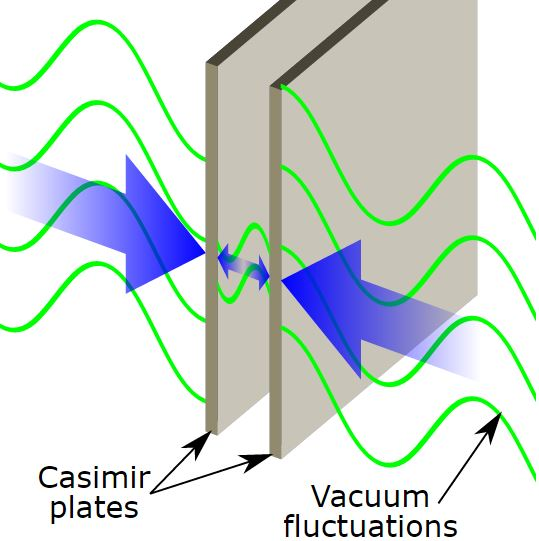
\includegraphics[width=4 cm]{pic/Casimir.jpg}
\caption{�����׶�ЧӦ.}
\label{Casimir}
\end{center}
\end{figure}

����, ��̬�ܵij���, ��ζ��������ν�����Ҳ������������ô�տ���Ҳ��. ���������֮����������, ��Ϊ�����׶�ЧӦ; ��ЧӦ, �Ϳ����õ�ų����������˵��. ��������ƽ�н��������Ϊ~$d$, ��ƽ����~$x-y$ ƽ��; ����������, Ϊ~$A$. �������ǿɵ�~$d$ �����, �Ե�ų�, ��λ����ϵĻ�̬����Ϊ
\begin{align}
\frac{\langle E\rangle}{A}=2\int \frac{dk_xdk_y}{(2\pi)^2}\sum_{n=1}^\infty\frac{\hbar}{2}\omega_n=2\int \frac{dk_xdk_y}{(2\pi)^2}\sum_{n=1}^\infty\frac{\hbar}{2}c\sqrt{k^2_x+k^2_y+\left(\frac{n\pi}{d}\right)^2};
\end{align}
���ж�~$z$ �������Dz���������ѧ������, ��~$x, y$ �������Dz��������ڱ߽�����, ��~$k=\frac{2\pi}{L}$. ��������ֵ�Ƿ�ɢ��; ���Dz���~zeta ���滯, ��ת�Ƶ�������֮��, ����
\begin{align}
\frac{\langle E(s)\rangle}{A}=&\hbar\int \frac{dk_xdk_y}{(2\pi)^2}\sum_{n=1}^\infty\omega_n|\omega_n|^{-s}\nonumber\\
=&\frac{\hbar c^{1-s}}{4\pi^2}\sum_n\int_0^\infty 2\pi q dq\Big|q^2+\frac{n^2\pi^2}{d^2}\Big|^{(1-s)/2}\nonumber\\
=&-\frac{\hbar^{1-s}\pi^{2-s}}{2a^{3-s}}\frac{1}{3-s}\sum_n|n|^{3-s}.
\end{align}
������DZ�����
\begin{align}
\frac{\langle E\rangle}{A}=\lim_{s\rightarrow0}\frac{\langle E(s)\rangle}{A}=-\frac{\hbar c\pi^2}{6a^3}\zeta(-3)=-\frac{\hbar c\pi^2}{720a^3};
\end{align}
�����õ���~$\zeta(-3)=\frac{1}{120}$. ���ǿ����׶�������
\begin{align}
\frac{F_c}{A}=-\frac{\partial}{\partial d}\frac{\langle E\rangle}{A}=-\frac{\hbar c\pi^2}{240a^4}.
\end{align}



\subsection{������̬����������һ������, ����ռ䳡������׹�ϵ, Э�����ʽ}

~~~~
��������ѧ����������֪, ǰ�Ķ����ռ䳡����Ķ��׹�ϵ, ��ζ��~$a^\dag_{\bm{p}}$ �����ӵIJ������, ��~$a^\dag_{\bm{p}}|0\rangle=|\bm{p}\rangle$. ���ǿ�֪~$\langle0|[a_{\bm{p}},a^\dag_{\bm{p}'}]|0\rangle=\langle0|a_{\bm{p}}a^\dag_{\bm{p}'}|0\rangle=\langle\bm{p}|\bm{p}'\rangle=(2\pi)^3\delta^3(\bm{p}-\bm{p}')$. ��һ����,
\begin{align}
\phi(x)|0\rangle=&\phi^\dag(x)|0\rangle=\int\frac{d^3\bm{p}}{(2\pi)^3\sqrt{2E_{\bm{p}}}}e^{ipx}a^\dag_{\bm{p}}|0\rangle\nonumber\\
=&\int\frac{d^3\bm{p}}{(2\pi)^3\sqrt{2E_{\bm{p}}}}e^{ipx}|\bm{p}\rangle:=|x\rangle
\end{align}
�ͱ�ʾ��~$x$ �㴦����һ���ɷֽ�Ϊ���ģ���ӵ�����; ע����������̬�������ȱ���, �����κι���ϵ, ������ͬ��������. �ɴ˿��Եõ�\footnote{��Ϊ�Ա�, $\delta^3(\bm{r}-\bm{r}')=\frac{1}{(2\pi\hbar)^3}\int d^3\bm{p}e^{i\bm{p}\cdot(\bm{r}-\bm{r}')/\hbar}$.}
\begin{align}
\langle x|y\rangle:=\langle0|\phi(x)\phi(y)|0\rangle=\int\frac{d^3\bm{p}}{(2\pi)^32E_{\bm{p}}}e^{-ip(x-y)}:=D(x-y)
\end{align}
���������Ӵ�~$y$ ��~$x$ �Ĵ���. ע��˴�����ϵ���������ȱ���.

��ѧ������֪��, $\delta(f(x)-f(x_0))=\frac{1}{|f'(x_0)|}\delta(x-x_0)$, �ʿɼ����
\begin{align}
\delta^3(\bm{p}-\bm{p}')=&\delta^3(\bm{p}_b-\bm{p}'_b)\frac{dp^i_b}{dp^i}=\delta^3(\bm{p}_b-\bm{p}'_b)\gamma(1+\beta\frac{dE_{\bm{p}}}{dp^i})\nonumber\\
=&\delta^3(\bm{p}_b-\bm{p}'_b)\frac{\gamma}{E_{\bm{p}}}(E_{\bm{p}}+\beta p^i)=\delta^3(\bm{p}_b-\bm{p}'_b)\frac{E_{\bm{p}_b}}{E_{\bm{p}}};
\end{align}
�����õ�������������άʸ���������ȱ任ʽ~(\ref{titi}). ���������̿ɼ�, $E_{\bm{p}}\delta^3(\bm{p}-\bm{p}')$ �������Ȳ����. ������ƽ�ֵ��������������, �͵�~$\sqrt{2E_{\bm{p}}}a_{\bm{p}}$ �������ȱ���. �ڱ���~K-G �����̽�~(\ref{so of kg}) �������ȱ���ʱ, ǰ�����ᵽ���������, ���ڵ��Խ��\footnote{�����һ������������ʵ�ռ�ת���µı仯��Ϊ���������Ƶķ�ʽ����, ����~$U(\Lambda_p)\sqrt{2E_{\bm{p}}}a_{\bm{p}}=\sqrt{2E_{\Lambda^{-1}_p\bm{p}}}a_{\Lambda^{-1}_p\bm{p}}=\sqrt{2E_{\bm{p}}}a_{\bm{p}}$.}.~%; ������~$U(\Lambda_p)a_{\bm{p}}=\frac{\sqrt{2E_{\Lambda^{-1}_p\bm{p}}}}{\sqrt{2E_{\bm{p}}}}a_{\Lambda^{-1}_p\bm{p}}$.}
%
%\footnote{�����һ������������ʵ�ռ�ת���µı仯��Ϊ���������Ƶķ�ʽ����, ����~$\sqrt{2E_{\bm{p}}}a_{\bm{p}}\rightarrow\sqrt{2E'_{\bm{p}}}a'_{\bm{p}}=\sqrt{2E_{\bm{p}}}a_{\bm{p}}= U(\Lambda_p)\sqrt{2E_{\bm{p}}}a_{\bm{p}}=\sqrt{2E_{\Lambda^{-1}_p\bm{p}}}a_{\Lambda^{-1}_p\bm{p}}$~(������ʾ~$M=I$, �Ա���~$\phi'(x)=U(\Lambda)\phi(x)=\phi(\Lambda^{-1}x)$); ������~$a'_{\bm{p}}=a_{\bm{p}}=\frac{\sqrt{2E_{\Lambda^{-1}_p\bm{p}}}}{\sqrt{2E'_{\bm{p}}}}a_{\Lambda^{-1}_p\bm{p}}=\frac{\sqrt{2E_{\Lambda^{-1}_p\bm{p}}}}{\sqrt{2E_{\bm{p}}}}a_{\Lambda^{-1}_p\bm{p}}$, �Ӷ�~$a_{\bm{p}}\rightarrow a'_{\bm{p}}=a_{\bm{p}}=U(\Lambda_p)a_{\bm{p}}=\frac{\sqrt{2E_{\Lambda^{-1}_p\bm{p}}}}{\sqrt{2E'_{\bm{p}}}}a_{\Lambda^{-1}_p\bm{p}}=\frac{\sqrt{2E_{\Lambda^{-1}_p\bm{p}}}}{\sqrt{2E_{\bm{p}}}}a_{\Lambda^{-1}_p\bm{p}}$. ע���һ���ﲢ������ʲô��ʾ, ��ֻ��ʾһ�ֱ仯��ϵ; ��ͬ���ȵ���~boost �µ���Ϊ����; ���Բ�����~$A'^\mu(x)=U(\Lambda)A^\mu(x)={\Lambda^\mu}_\nu A^\nu(\Lambda^{-1}x)$ ��һ�Ƚ����.}
%
%��Ʋ�����º�����ij��, ���������Ϻ�����ij��
%$\sqrt{2E_{\bm{p}}}a_{\bm{p}}\rightarrow U(\Lambda_p)\sqrt{2E_{\bm{p}}}a_{\bm{p}}=\sqrt{2E_{\Lambda_p\bm{p}}}a_{\Lambda_p\bm{p}}=\sqrt{2E_{\bm{p}}}a_{\bm{p}}$, �Ӷ�~$a_{\bm{p}}=\frac{\sqrt{2E_{\Lambda_p\bm{p}}}}{\sqrt{2E_{\bm{p}}}}a_{\Lambda_p\bm{p}}$, $a_{\bm{p}}\rightarrow a_{\Lambda_p\bm{p}}=U(\Lambda_p)a_{\bm{p}}=\frac{\sqrt{2E_{\bm{p}}}}{\sqrt{2E_{\Lambda_p\bm{p}}}}a_{\bm{p}}$
%
%����DZ���, �����ڱ�������.
%
%������Ϊʲô���б���, ʸ����? ��ΪȺ��ƽӹ��ʾ, ������ʾ.
%
����, ��������̬
\begin{align}
|p^\rangle:=|p^\mu\rangle:=\sqrt{2E_{\bm{p}}}a^\dag_{\bm{p}}|0\rangle=\sqrt{2E_{\bm{p}}}|\bm{p}\rangle
\end{align}
���������Ȳ����; ���ɵ����һ��Ϊ~$\langle p|p'\rangle=2E_{\bm{p}}(2\pi)^3\delta^3(\bm{p}-\bm{p}')$. ��������֪ʶ, ���ǾͿɼ����
\begin{gather}
\langle p|x\rangle=e^{ipx},~\langle x|p\rangle=e^{-ipx};
\end{gather}
���ǾͿɵõ�
\begin{gather}
I=\int\frac{d^3\bm{p}}{(2\pi)^32E_{\bm{p}}}|p\rangle\langle p|,~I=2E_{\bm{p}}\int d^3\bm{x}|x\rangle\langle x|.
\end{gather}
%����������������Dz�����.
����ѡ����ʱ��~$\langle \bm{p}|\bm{x}\rangle=e^{-i\bm{p}\cdot\bm{x}},~\langle \bm{x}|\bm{p}\rangle=e^{i\bm{p}\cdot\bm{x}}$, �Լ�~$\langle\bm{x}|\bm{y}\rangle=\delta^3(\bm{x}-\bm{y})$, �򻹿ɼ����
\begin{gather}
I=\int\frac{d^3\bm{p}}{(2\pi)^3}|\bm{p}\rangle\langle\bm{p}|,~I=\int d^3\bm{x}|\bm{x}\rangle\langle\bm{x}|.
\end{gather}
���ƸղŸ�����~$|p\rangle$ ��~$|\bm{p}\rangle$ �Ĺ�ϵ, ����Ҳ�ɸ���~$\sqrt{2E_{\bm{p}}}|x\rangle\leftrightarrow|\bm{x}\rangle$.


Ӧ��ǰһ�����Ǹ����Ķ����ռ䳡����Ķ��׹�ϵ, ���Ѽ��������ռ�:
\begin{align}
[\phi(x),\phi(y)]&=\int\frac{d^3\bm{p}}{(2\pi)^32E_{\bm{p}}}\left[e^{-ip(x-y)}-e^{-ip(y-x)}\right]\nonumber\\
&=D(x-y)-D(y-x),\\
[\pi(x),\pi(y)]&=\int\frac{d^3\bm{p}}{(2\pi)^3}\frac{E_{\bm{p}}}{2}\left[e^{-ip(x-y)}-e^{-ip(y-x)}\right],\\
[\phi(x),\pi(y)]&=\frac{i}{2}\int\frac{d^3\bm{p}}{(2\pi)^3}\left[e^{-ip(x-y)}+e^{-ip(y-x)}\right];
\end{align}
������һ�����׹�ϵ, ���ΪЭ����׹�ϵ, �������ȱ���; ����������. ��Ӧ�ñ��ڸ�������ά����ά���˱�����, ���Ǽ���������ʽ�Ӷ�����ʱ���׹�ϵ
\begin{gather}
[\phi(\bm{x}),\phi(\bm{y})]=0,~[\pi(\bm{x}),\pi(\bm{y})]=0,\\
[\phi(\bm{x}),\pi(\bm{y})]=i\delta^3(\bm{x}-\bm{y}).
\end{gather}

���, ��ʽ~(\ref{diejia}) ���ֳ����⺭����д����
\begin{align}
a_{\bm{p}}&=\sqrt{2E_{\bm{p}}}\int d^3\bm{x}e^{ipx}\frac{1}{2}\left[\phi(x)+\frac{i\pi(x)}{E_{\bm{p}}}\right],\\
a^\dag_{\bm{p}}&=\sqrt{2E_{\bm{p}}}\int d^3\bm{x}e^{-ipx}\frac{1}{2}\left[\phi(x)-\frac{i\pi(x)}{E_{\bm{p}}}\right];
\end{align}
�����������ռ䳡���ĺ�ʱ���׹�ϵ, ����ʽ���ǿ����Ƴ������ռ�Ķ���ʽ��.


\subsection{���������΢������ɶ����ӳ��۵�Ҫ��: ���������������/�Գ���/ͳ�ƵĹ�ϵ}

~~~~
��������۱���, ��ʱ��������������¼�, ���Խ����ź�����; ����ռ�����¼��Dz����Ե�, ���߽�ʧȥȷ�����Ⱥ����. ���Ϊ������������綨��΢������������. ��ӳ�����ӳ�����, �����Ҫ��, ��ռ�������ϵ���ѧ�����, �����ǻ�����׵�, ��
\begin{align}
[\mathcal{O}(x),\mathcal{O}(y)]=0,~\textrm{when}~(x-y)^2<0.
\end{align}
���׿���, ��������ӳ�������ѧ������ij������, ����Ҫ��, �������ȡ�Ķ��׹�ϵ����, Ҫʹ������ռ����, ���IJ�ȡͬ�����׹�ϵ��Э������ʽ���Ϊ��. ����һС�ڵļ���������֪~$[\phi(x),\phi(y)]=D(x-y)-D(y-x)$; ����ռ����, �˶���ʽ��ֵ��ȷ�ǵ������. ͬʱҲ�ɿ���, ��������ȡΪ������ʽ, ����ռ�������ǵķ����׽����Ȼ��Ϊ��. �ǹ�����Ϊ��ı�������ȡ���׹�ϵ. ͬ��, ����һ�µ����˳�������Ҳ������, �Ծ���~$1/2$ ����������, ����ռ����, ���ȡ������ʽ�ij���Э������ʽ���Ϊ��. �ǹ�����Ϊ~$1/2$ �����ӱ�ȡ�����׹�ϵ.

��һ��, ���ǽ�����, ���������������ɵ�Ҫ��, ������������������, ���뱻������׹�ϵ; ���Ӳ����������ӽ����ǶԳƵ�, ����ϵ���㲣ɫ-����˹̹ͳ��; ���������ӳ�Ϊ��ɫ��. �����а���������������, ���뱻���跴���׹�ϵ; ���Ӳ����������ӽ����Ƿ��ԳƵ�, ����ϵ�������-������ͳ��; ���������ӳ�Ϊ������.




\subsection{�����Ӵ������ʷ�: ����������; ��ά������~$\delta$ ����}

~~~~ǰ��������֪��~$\langle x|y\rangle=D(x-y)$ ��ʾ���Ӵ�λ�ÿռ��~$y$ �㵽~$x$ ��Ĵ���; ���������Dz�û�мƼ�ʱ����Ⱥ�. ���ǽ�ʱ���Ⱥ�Ĵ�����ϵ~$D_F(x-y):=\langle0|T\phi(x)\phi(y)|0\rangle$, ��Ϊ����������. ����, $D_R(x-y):=\theta(x^0-y^0)\langle0|[\phi(x),\phi(y)]|0\rangle$ ��Ϊ�Ƴٸ��ֺ���, �ȵ�. ����, �����Է���������Ϊ��, �����н�һ������.
\begin{align}
&D_F(x-y)=\langle0|T\phi(x)\phi(y)|0\rangle\nonumber\\
=&\theta(x^0-y^0)\langle0|\phi(x)\phi(y)|0\rangle+\theta(y^0-x^0)\langle0|\phi(y)\phi(x)|0\rangle\nonumber\\
=&\theta(x^0-y^0)\int\frac{d^3\bm{p}}{(2\pi)^32E_{\bm{p}}}e^{-ip(x-y)}+\theta(y^0-x^0)\int\frac{d^3\bm{p}}{(2\pi)^32E_{\bm{p}}}e^{-ip(y-x)}\nonumber\\
=&\theta(x^0-y^0)\int\frac{d^3\bm{p}}{(2\pi)^32E_{\bm{p}}}e^{-ip(x-y)}\Big|_{p^0=E_{\bm{p}}}\nonumber\\
&~~~~~~~~~~~~~~~~~~~~~~~~~~~~~~~~-\theta(y^0-x^0)\int\frac{d^3\bm{p}}{(2\pi)^3(-2E_{\bm{p}})}e^{-ip(x-y)}\Big|_{p^0=-E_{\bm{p}}}\nonumber\\
=&\int\frac{d^3\bm{p}}{(2\pi)^3}\int\frac{dp^0}{2\pi i}\frac{-1}{p^2-m^2}e^{-ip(x-y)}~\textrm{with~Feynman~prescription}\nonumber\\
=&\int\frac{d^4p}{(2\pi)^4}\frac{i}{p^2-m^2}e^{-ip(x-y)}~\textrm{with~Feynman~prescription};
\end{align}
%����������ɫɢ��ϵ��, ���ַ���, û�а���ɫɢ��ϵ��; ��Ȼ, �������ֳ��������ս��, �õ������Ӵ�����ϵ, ������ɫɢ��ϵ��.
%�������ص�������ƽ��, ����ʵ�����, �ͳ����������.
\begin{figure}[!h]
\begin{center}
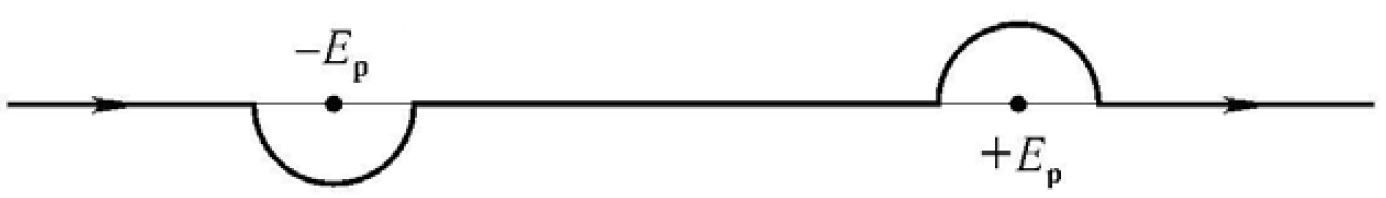
\includegraphics[width=7 cm]{pic/feynman.jpg}
\caption{��������: ���������ӻ�Χ����ѡȡ.}
\label{feynman}
\end{center}
\end{figure}
�����õ�����������~$\oint_l f(z)dz=2\pi i\sum_k f(a_k)$, ������Χ����ѡ���ʾ��ͼ~\ref{feynman} ��, ��Ϊ��������. ע�����������еĽ���������ζ�Ŷ���ά�����Ļ���, ����Ҫ����ά��������ɫɢ��ϵ, ������Ϊ���ֵ�������. ��Ȼ, ��~$\int\frac{d^4p}{(2\pi)^4}\frac{i}{p^2-m^2}e^{-ip(x-y)}$ ����Χ���IJ�ͬѡ��, ��������ͬ�Ĵ�����; ��ͼ~\ref{ret} �������Ƴٸ��ֺ���.
\begin{figure}[!h]
\begin{center}
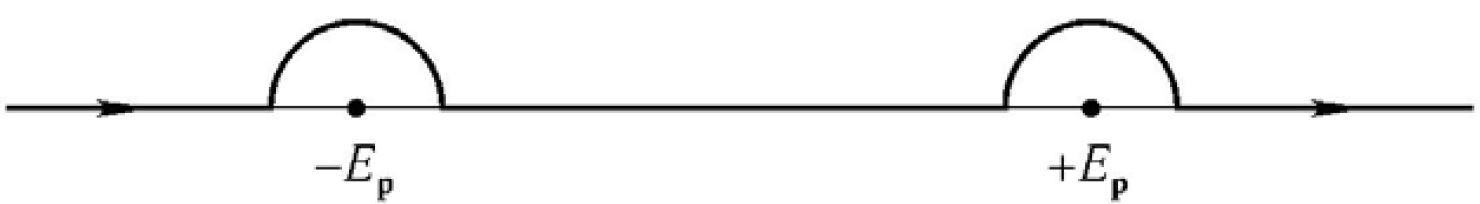
\includegraphics[width=7 cm]{pic/ret.jpg}
\caption{�Ƴ��ƻ���Χ����ѡȡ.}
\label{ret}
\end{center}
\end{figure}

\noindent ���ڷ���������, һ�������ֻ�������¼Ƿ�:
\begin{align}
D_F(x-y)=\int\frac{d^4p}{(2\pi)^4}\frac{i}{p^2-m^2+i\epsilon}e^{-ip(x-y)},
\end{align}
���Ϊ~$\epsilon$ ����.

ע��, �����ӵı���ʽ, �Է���������Ϊ��, ��������~$D_F(p):=\frac{i}{p^2-m^2+i\epsilon}$ ����ά����Ҷ�任; ���к��߼��������ڶ����ռ�ı���ʽ. �Ѵ����Ӵ���~K-G ����, �ɵ�
\begin{align}
(\partial^2+m^2)D_F(x-y)=-i\int\frac{d^4p}{(2\pi)^4}e^{-ip(x-y)}:=-i\delta^4(x-y),
\end{align}
���������dz����̵ĸ��ֺ���. ����������, ͨ����Ӽ����~$D_F(x-y)=\int\frac{d^4p}{(2\pi)^4}D_F(p)e^{-ip(x-y)}$ ������֮, �������ֱ�ӵõ�~$D_F(p)$ ����~$D_F(x-y)$ �ı���ʽ. --����ʽ��, ���Ƕ�����λ�ÿռ���ά������~$\delta$ ����
\begin{align}
\delta^4(x-y)=&\delta(x^0-y^0)\delta^3(\bm{x}-\bm{y})=\delta(x^0-y^0)\frac{1}{(2\pi)^3}\langle\bm{x}|\bm{y}\rangle\nonumber\\
=&\int\frac{d^4p}{(2\pi)^4}e^{-ip(x-y)}.
\end{align}
ע��, ����ǰ���Ѿ�˵��������, ��������ά�����Ļ���, ��Ҫ��ɫɢ��ϵ, ������Ȼ�ֹ��ɻش�������. ��Ϊ�Ա�, �����Ƕ���~$\langle p|p'\rangle=2E_{\bm{p}}\langle\bm{p}|\bm{p}'\rangle=2E_{\bm{p}}(2\pi)^3\delta^3(\bm{p}-\bm{p}'):=(2\pi)^4\delta^4(p-p')$, ��ȡ~$I=\int d^4x|x\rangle\langle x|$, �Ϳɵõ���ά�����ռ�ĵ�����~$\delta$ ��������:
\begin{align}
\delta^4(p-p')=\int\frac{d^4x}{(2\pi)^4}e^{-i(p-p')x}.
\end{align}


%���ֺ����Ļ���, ��������ɫɢ��ϵ, ����, ����˴�������. Ҳ����˵�������������.

���Ժ���໥���ó�����, ��ij�����̵�ij�׽���, ����ͨ���Ὣ����Ӧ�Ľ�������ʽ��ͼ�εķ�������. ��Щͼ��, ��Ϊ����ͼ; ͼ���������ʽ֮��Ķ�Ӧ����, ��Ϊ��������. ����, ��򵥵ķ���ͼ, ���������������һ���߶α�ʾ����������:
\begin{align}\label{green f}
D_F(x-y)=\begin{aligned}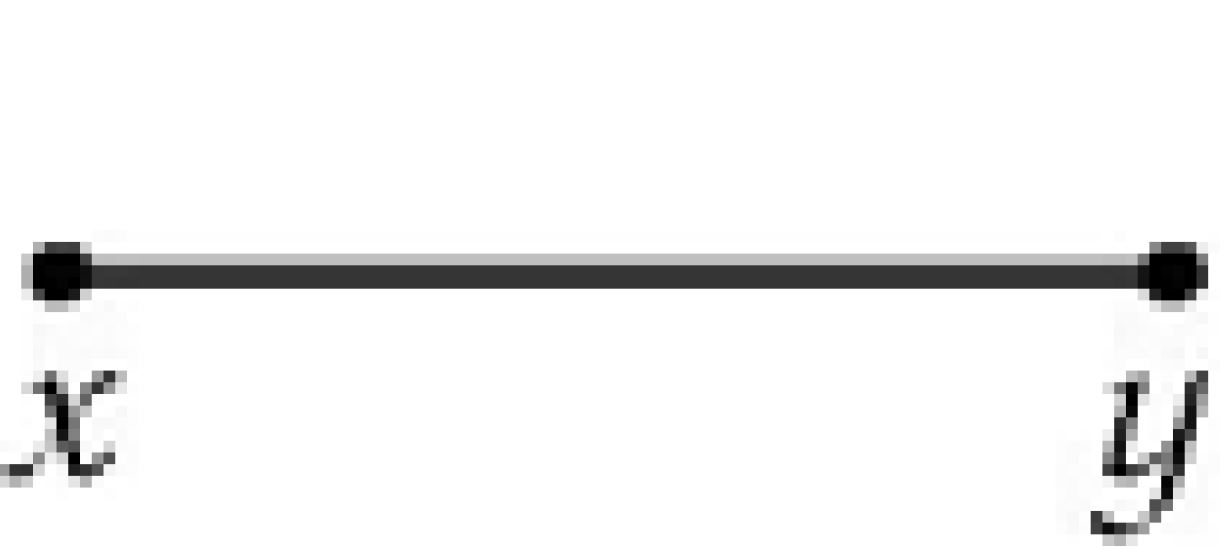
\includegraphics[width=1.3 cm]{pic/pp.jpg}\end{aligned}~.
\end{align}


%���ڱ�������, ǡǡ��Ϊ���Ǵ˴���~$p^2=m^2$, ���������ڿǵ�, ���Dz�֪�����Ĵ������������ǿɱ�̽������ʵ������. ��Ϊ�Ա�, ���໥���ó�����, �������Ӳ��ڿ�, �������, �Dz���̽���.

%���������������ɳ����еó�������Ҫ�Ľ��֮һ, �������պ���໥���ó����е�ɢ������ļ������ֱ�ӵĹ�ϵ. ����, �����ɳ����������Ӿ���������ʽ��~$\langle\Omega|T\phi_H(x)\phi_H(y)|\Omega\rangle$--��Ϊ������������ֺ���--Ҳ����������ĵ�������֮һ. ��ʱ����Ҫ����, ������ΰѹ������������ɳ����еķ�����������ϵ����������.


%�������Ƿ��漰�������?



\subsection{��������: �������������к�, $\pi^\pm$ ����}

~~~~������֪, ������ǰ���ֽ�����ʵ������, ��������~$\pi^0$ ����. ����һ���������ɵĽ���, ��Ϊ~$\pi^\pm$; ��ǰ������֪, �������ǵļ�Ϊ��������. ���������������ܶ�, �Լ���֮���µij����˶�����, �������Ľ�Ϊ:
\begin{gather}
\mathcal{L}=\partial_\mu\phi^\dag\partial^\mu\phi-m^2\phi^\dag\phi,\\
(\partial^2+m^2)\phi=0,~(\partial^2+m^2)\phi^\dag=0;\\
\phi(x)=\int\frac{d^3\bm{p}}{(2\pi)^3\sqrt{2E_{\bm{p}}}}\left(a_{\bm{p}}e^{-ipx}+b^\dag_{\bm{p}}e^{ipx}\right),\\
\phi^\dag(x)=\int\frac{d^3\bm{p}}{(2\pi)^3\sqrt{2E_{\bm{p}}}}\left(a^\dag_{\bm{p}}e^{ipx}+b_{\bm{p}}e^{-ipx}\right);
\end{gather}
����~$a^\dag_{\bm{p}}$ ��~$b^\dag_{\bm{p}}$ ���������ֱ��������ɵ���������. �������������Լ������ܶȾ���
\begin{gather}
\pi=\frac{\partial\mathcal{L}}{\partial\dot{\phi}}=\dot{\phi}^\dag,~\pi^\dag=\frac{\partial\mathcal{L}}{\partial\dot{\phi}^\dag}=\dot{\phi};\\
\mathcal{H}=\pi\dot{\phi}+\pi^\dag\dot{\phi}^\dag-\mathcal{L}.
\end{gather}
���豾�����¶��׹�ϵ, ����ʵ����ϵ�����ӻ�:
\begin{gather}
[a_{\bm{p}},a^\dag_{\bm{p}'}]=(2\pi)^3\delta^3(\bm{p}-\bm{p}'),~[b_{\bm{p}},b^\dag_{\bm{p}'}]=(2\pi)^3\delta^3(\bm{p}-\bm{p}');\\
\Leftrightarrow~[\phi(\bm{x}),\pi(\bm{y})]=i\delta^3(\bm{x}-\bm{y}),~[\phi^\dag(\bm{x}),\pi^\dag(\bm{y})]=i\delta^3(\bm{x}-\bm{y});
\end{gather}
�����Ķ��׽�Ϊ��. ����Э����׹�ϵ�����׶���Ϊ~
\begin{gather}
[\phi(x),\phi(y)]=0,~[\phi^\dag(x),\phi^\dag(y)]=0,\\
[\phi(x),\phi^\dag(y)]=D_a(x-y)-D_b(y-x).
\end{gather}
���������Ĵ󲿷���ѧ������ʵ���������Ƕ�Ӧһ�µ�; ������Ҫ�о��������������Ĺ淶��. ����������Ӧ������淶������غ����ܶ�Ϊ
\begin{align}
j^\mu_{(q)}=&\frac{q}{i}\left(\frac{\partial\mathcal{L}}{\partial\partial_\mu\phi}\phi-\phi^\dag\frac{\partial\mathcal{L}}{\partial\partial_\mu\phi^\dag}\right)\nonumber\\
=&iq(\phi^\dag\partial^\mu\phi-\phi\partial_\mu\phi^\dag);
\end{align}
���������ڷ�����ѧ�����Ǿ����������. �������ǿ���������������غ��Ϊ
\begin{align}
Q=&\int d^3\bm{x}j^0_{(q)}=iq\int d^3\bm{x}(\phi^\dag\partial^0\phi-\phi\partial_0\phi^\dag)\nonumber\\
=&q\int\frac{d^3\bm{p}}{(2\pi)^3}(a^\dag_{\bm{p}}a_{\bm{p}}-b^\dag_{\bm{p}}b_{\bm{p}})
\end{align}
�ɴ�ȷ��, $a^\dag_{\bm{p}}$ ��~$b^\dag_{\bm{p}}$ ���������Ӻ��Ե�ȷ�෴.





\newpage

\section{��������: 1/2-�����������к�, �����˷�����}
\subsection{�����˷��̼��乲���, ����-�����˱���, ������̵������ܶ�, ��Լ���ɷ�����, ��ʸ��}
~~~~ǰ��Ⱥ��һ����, �������ϸ񵼳���������ķ���~$(\gamma^\mu p_\mu-m)\psi=0$. ������~$p_\mu=i\partial_\mu$, ��ɵõ����ӷ���
\begin{align}
(i\gamma^\mu\partial_\mu-m)\psi=0;
\end{align}
��Ϊ�����˷���. �ܵ��µ����˷��̵������ܶ�Ϊ
\begin{align}
\mathcal{L}=\bar{\psi}(i\gamma^\mu\partial_\mu-m)\psi;
\end{align}
%ǡ��ǰ�ķ���, �������ܶ���ֵΪ�㴦, ȡ���˶�����; ��Ի
�ɼ���ʵ�˶�ʹ���������ܶ�Ϊ��. �����~$\bar{\psi}$ Ӧ���������շ��̼��ɵ�ǰ�������˷���; �����~$\psi$ Ӧ�����Ϸ���, �ɵ�
\begin{align}
i\partial_\mu\bar{\psi}\gamma^\mu+m\bar{\psi}=0;
\end{align}
�˼������˷��̵Ĺ����. ��Ȼ, ��ʽҲ���ɵ����˷������ݻ����. ��������˵��, �κγ�����Ҫ����~Klein-Gordon ���̵�. �Ե����˷���������֤����~$-(i\gamma^\nu\partial_\nu+m)(i\gamma^\mu\partial_\mu-m)\psi=(\gamma^\mu\gamma^\nu\partial_\mu\partial_\nu+m^2)\psi=(\partial^2+m^2)\psi=0$.

�����Ѿ�֤���˵����˷��̶���ɢ�任�ǶԳƵ�; ����, ������֤�������˷��������������ȱ任�µIJ�����. ��ʵ��, ԭ���, һ����ֻҪ������������ʸ������, ����Ƕ������ȱ任����ı���. �����������ǻ��Ǿ�����һ��. ����ϵ������ϵ����һ��������ת��, ����
\begin{align}
(i\gamma^\mu\partial_\mu-m)\psi=0&\rightarrow\left(i\Lambda_{\frac{1}{2}}\gamma^\mu\Lambda^{-1}_{\frac{1}{2}}{\Lambda_\mu}^\nu\partial_\nu-m\right)\Lambda_{\frac{1}{2}}\psi(\Lambda^{-1}x)\nonumber\\
&=\left[i\Lambda_{\frac{1}{2}}\gamma^\mu\Lambda^{-1}_{\frac{1}{2}}\partial_\mu-m\right]\Lambda_{\frac{1}{2}}\psi(\Lambda^{-1}x)\nonumber\\
&=\Lambda_{\frac{1}{2}}(i\gamma^\mu\partial_\mu-m)\psi(\Lambda^{-1}x)=0;
\end{align}%���ԭ���ķ��̳���, �����ǹ۲�ϵ��������תһ�º�, ��ϵ���������ķ���.
�ɴ˿ɼ�, �����������ȱ任��, �����˷��̵�ȷ�Dz����.

����, ��Ⱥ��һ�����Ƶ�ʱ, $\psi$ �����·����Ǿ���ȷ����������������; ��Ӧ�õ���~$\gamma^\mu$ �򷽺͵ľ�����ʽ, ���������������������µ�. ��ѧ������֪��, ÿһ������~$\gamma^\mu$ �Ĵ����ľ���, ���ǵ����˷��̵�һ����ʾ. ��ȡ~$\gamma^0=\left[\begin{array}{cc}1&0\\0&-1\end{array}\right]$, ��ȡ~$\gamma^i$ ����ʽ����������е���ͬ, ���ѷ���, ������һ�����, ��������~$\gamma^\mu$ �Ĵ�����. �����˱�ʾ�ı���, ���dz�Ϊ����-�����˱���. ��ʱ, �����˷��̵ľ�����ʽ����
\begin{align}
\left[\begin{array}{cc}
E-m&-\bm{\sigma}\cdot\bm{p}\\
\bm{\sigma}\cdot\bm{p}&-E-m
\end{array}\right]
\left[\begin{array}{c}\varphi\\\chi\end{array}\right]=0.
\end{align}
������֪, ����������Ϊ��ʱ, �����˷����˻�Ϊ�����������, �����������˻�Ϊ�����ֱ�����������̬���������. Ҳ����˵, �����ӵĶ���Զ���ھ�����ʱ, ������������Ƿ����. ͬ���ɿ���, �����Ӷ��ܽ�С, ����ԶС�ھ�����ʱ, ���õ����˱����Ƿ����.

�����������������������ʽ����������˳������ܶ�\footnote{���������൱����~$\psi=\left[\begin{array}{c}\psi_L\\\psi_R\end{array}\right]$. ��������~$\psi=\left[\begin{array}{c}L\\R\end{array}\right]$, ��~$\psi_L=\left[\begin{array}{c}L\\0\end{array}\right],~\psi_R=\left[\begin{array}{c}0\\R\end{array}\right]$, ��~$\psi=\psi_L+\psi_R,~\bar{\psi}\psi=R^\dag L+L^\dag R=\bar{\psi}_R\psi_L+\bar{\psi}_L\psi_R$; ��~$\bar{\psi}\gamma^\mu\psi=L^\dag\bar{\sigma}^\mu L+R^\dag\sigma^\mu R=\bar{\psi}_L\gamma^\mu\psi_L+\bar{\psi}_R\gamma^\mu\psi_R$.}:
\begin{align}
\mathcal{L}=\psi^\dag_L i\bar{\sigma}^\mu\partial_\mu\psi_L+\psi^\dag_R i\sigma^\mu\partial_\mu\psi_R-m(\psi_R^\dag\psi_L+\psi^\dag_L\psi_R).
\end{align}
��Ȼ, �������������������������. ������Ϊ��ʱ, �����˳������ܶ��˻�Ϊ�������������, ���߼������ֱ����������������˶�����������.

���ǿ��Խ������˷���дΪ~$i\gamma^0\partial_0\psi=(-i\gamma^i\partial_i+m)\psi$, �Ӷ�~$i\partial_0\psi=(-i\gamma^0\gamma^i\partial_i+\gamma^0m)\psi$; ����~$\gamma^0=\beta,~\alpha^i=\gamma^0\gamma^i$, ��͵�
\begin{align}
i\partial_0\psi=(-i\alpha^i\partial_i+\beta m)\psi;
\end{align}
�˼�����������д�µ���ʽ.







������̸һ����Լ���ɷ�����. %�����������Ǹ���, �����˱�ʾ��������Ⱥ��һ������ʾ; ��Դ��������Ϊ~$\gamma$ ����������~Clifford ������ѡ������Ӧ����.
������Ϊ~Clifford ����ѡȡ������ʾ����: $\gamma^0=
\left[\begin{array}{cc}
0&i\sigma^2\\
i\sigma^2&0
\end{array}\right],~
\gamma^1=
\left[\begin{array}{cc}
i\sigma^3&0\\
0&i\sigma^3
\end{array}\right],~
\gamma^2=
\left[\begin{array}{cc}
0&-\sigma^2\\
\sigma^2&0
\end{array}\right],~
\gamma^3=
\left[\begin{array}{cc}
-i\sigma^1&0\\
0&-i\sigma^1
\end{array}\right],$
��Ϊ��Լ���ɻ�, ��ɷ������ǵõ���������Ⱥ��һ��ʵ������ʾ; ��Ӧ�ı�ʾ�������ͳ�Ϊ��ά��������. ��Ȼ, ��ά���������ĺɹ���, ��~$C$ �任�����������~$\psi=\left[\begin{array}{c}\psi_L\\i\sigma^2\psi^*_L\end{array}\right]$. ���Ƿ�������������������, Ϊ��Լ���ɷ�����.

��֮, ������������������������, 1/2-�����������к�, �����, ��˵�, ��Ϊ�����˷�����; ������������������������, 1/2-�����������к�, ��Ϊ���������; ������ʵ����������������, 1/2-�����������޺�, ��Ϊ��Լ���ɷ�����.

���, �����ó�������һЩ��ѧ��. �����Ĺ���������������Ϊ
\begin{gather}
\pi=\frac{\partial\mathcal{L}}{\partial\dot{\psi}}=i\bar{\psi}\gamma^0=i\psi^\dag,\\
\mathcal{H}=\pi\dot{\psi}-\mathcal{L}=i\psi^\dag\dot{\psi}-\bar{\psi}(i\gamma^\mu\partial_\mu-m)\psi=\bar{\psi}(-i\gamma^i\partial_i+m)\psi.
\end{gather}
�ڷ�����ѧ��, ������֪�����Ķ�Ӧ����Ϊ�ڲ��Գ��ԵĹ淶�任���غ���Ϊ
\begin{align}
j^\mu_{(q)}=\frac{q}{i}\left(\frac{\partial\mathcal{L}}{\partial\partial_\mu\phi}\phi-\phi^\dag\frac{\partial\mathcal{L}}{\partial\partial_\mu\phi^\dag}\right)=q\bar{\psi}\gamma^\mu\psi;
\end{align}
�Ӷ����������غ�ɼ�~$Q=q\int d^3\bm{x}\bar{\psi}\gamma^0\psi=q\int d^3\bm{x}\psi^\dag\psi$. ������������������������ְ��෴�ķ������淶�任, ��~$\psi\rightarrow e^{iq_H\alpha\gamma^5}\psi,~\bar{\psi}\rightarrow\bar{\psi}e^{iq_H\alpha\gamma^5}$, --���ֳ�Ϊ�����任, --�����Ƶ�, ���ǿ����ô˶�Ӧ�ڴ˵���Ϊ
\begin{align}
j^\mu_{(q)A}=q_H\bar{\psi}\gamma^\mu\gamma^5\psi;
\end{align}
��֮Ϊ��ʸ��. ����ע��, ��Ϊ~$\partial_\mu(\bar{\psi}\gamma^\mu\gamma^5\psi)=2im\bar{\psi}\gamma^5\psi$, ��Ȼ����ֻ������Ϊ��ʱ�ų�Ϊ�غ���. ��ʵ��, �˼���������ӵ�����. �����Ҳ���, ��Ȼ��
\begin{align}
j^\mu_{(q)AL}=q_H\bar{\psi}\gamma^\mu P_L\psi,~j^\mu_{(q)AR}=q_H\bar{\psi}\gamma^\mu P_R\psi.
\end{align}





\subsection{�����˷��̵Ľ�, $u^s(p),~v^s(p)$, Jordan-wigner ���ӻ�: �����׹�ϵ�ĸ���, ����������}

~~~~���ǿ���ֱ�Ӷ���, ��Ϊ�ķ��������������ĵ����˷��̵Ľ���
\begin{align}
\psi(x)&=\int\frac{d^3\bm{p}}{(2\pi)^3\sqrt{E_{\bm{p}}}}\sum_s\left(a^s_{\bm{p}}u^s(p)e^{-ipx}+b^{s\dag}_{\bm{p}}v^s(p)e^{ipx}\right);\\
\bar{\psi}(x)&=\int\frac{d^3\bm{p}}{(2\pi)^3\sqrt{E_{\bm{p}}}}\sum_s\left(a^{s\dag}_{\bm{p}}\bar{u}^s(p)e^{ipx}+b^{s}_{\bm{p}}\bar{v}^s(p)e^{-ipx}\right).
\end{align}
��Ҫ֮��, ��Ҫ��������~$u^s(p),~v^s(p)$ ������. ����Ƶ����Ϊ��, ���Ƿ��̵���Ƶƽ�沨��~$u(p)e^{-ipx}:=(u_1,u_2)^Te^{-ipx}$ ���뷽��, ������������, ����
\begin{align}
\left[\begin{array}{cc}
-m&\sigma^\mu p_\mu\\
\bar{\sigma}^\mu p_\mu&-m
\end{array}\right]\left[\begin{array}{c}u_1\\u_2\end{array}\right]=0;
\end{align}
�ɴ�֪~$\frac{u_1}{u_2}=\frac{\sigma^\mu p_\mu}{m}=\frac{m}{\bar{\sigma}^\mu p_\mu}$. �ɴ�, Ϊ����ʽ�Գ�, ���Ǽ��ɽ�~$u(p)$ �Ľ��������; �����Ƶİ취Ҳ�ɽ�~$v(p)$ ������; ���ǵĽ��Ϊ
\begin{align}
u(p)=\left[\begin{array}{c}\sqrt{\sigma^\mu p_\mu}\xi\\\sqrt{\bar{\sigma}^\mu p_\mu}\xi\end{array}\right],~v(p)=\left[\begin{array}{c}\sqrt{\sigma^\mu p_\mu}\eta\\-\sqrt{\bar{\sigma}^\mu p_\mu}\eta\end{array}\right];
\end{align}
����~$\xi^{s\dag}\xi^r=\delta^{sr},~\eta^{s\dag}\eta^r=\delta^{sr};~s,r=1,2$. ע�⵱���Ӿ�ֹʱ, ������~$u(\bm{p}=0)=\sqrt{m}(\xi,\xi)^T,~v(\bm{p}=0)=\sqrt{m}(\eta,-\eta)^T$. ���ǽ�ȷ��, $\xi^s$ �����˵��ӵ�����״̬; ����˵, $\xi^1=(1,0)^T,~\xi^2=(0,1)^T$. ����, ���Ƿdz����׼����:
\begin{gather}
u^{s\dag}(p)u^r(p)=2E_{\bm{p}}\delta^{sr},~\bar{u}^{s}(p)u^r(p)=2m\delta^{sr};\\
v^{s\dag}(p)v^r(p)=2E_{\bm{p}}\delta^{sr},~\bar{v}^{s}(p)v^r(p)=-2m\delta^{sr};\\
\bar{u}^{s}(p)v^r(p)=\bar{v}^{s}(p)u^r(p)=0;\\
u^{s\dag}(\bm{p})v^r(-\bm{p})=v^{s\dag}(\bm{p})u^r(-\bm{p})=0;\\
\sum_{s=1}^2u^s(p)\bar{u}^s(p)=\gamma^\mu p_\mu+m,~\sum_{s=1}^2v^s(p)\bar{v}^s(p)=\gamma^\mu p_\mu-m.
\end{gather}
��Ȼ~$\bar{u}^{s}(p)u^r(p)$ ��~$\bar{v}^{s}(p)v^r(p)$~�������Ȳ����.



ǰ������½�ͨ�����ϵ������������, ������ɵ�����, �����ӱ��뱻���跴���׹�ϵ, --����Ϊ~Jordan-Wigner ���ӻ�; �ʱ�����
\begin{gather}
\{a^{s}_{\bm{p}},a^{r\dag}_{\bm{p}'}\}=(2\pi)^3\delta^3(\bm{p}-\bm{p}')\delta_{sr},\\
\Leftrightarrow~\{\psi_\alpha(\bm{s}),\psi^\dag_{\beta}(\bm{y})\}=\delta^3(\bm{x}-\bm{y})\delta_{\alpha\beta}.
\end{gather}
��ʵ��, ����Ҳ������, ֻ�б����跴���׹�ϵ, �����ӵ���ѧ�����ܵõ��������. ������ϵ��������Ϊ
\begin{align}
H=&\int d^3\bm{x}\bar{\psi}(-i\gamma^i\partial_i+m)\psi=\int d^3\bm{x}i\psi^\dag\dot{\psi}\nonumber\\
=&\int\frac{d^3\bm{p}}{(2\pi)^3}\sum_sE_{\bm{p}}(a^{s\dag}_{\bm{p}}a^{s}_{\bm{p}}+b^{s\dag}_{\bm{p}}b^{s\dag}_{\bm{p}}).
\end{align}
�����糡���ܵ��
\begin{align}
Q=q\int d^3\bm{x}\bar{\psi}\gamma^0\psi=q\int d^3\bm{x}\psi^\dag\psi=\int\frac{d^3\bm{p}}{(2\pi)^3}\sum_sq(a^{s\dag}_{\bm{p}}a^{s}_{\bm{p}}-b^{s\dag}_{\bm{p}}b^{s\dag}_{\bm{p}}).
\end{align}
������������~$S^k=\int d^3\bm{x}\pi\frac{-i}{2}\Sigma^k\psi=\int d^3\bm{x}\psi^\dag\frac{1}{2}\Sigma^k\psi$; �����ڶ���������չ��, ��ɷ���~$\xi=(1,0)^T,~(0,1)^T$ �ֱ��������~$1/2,~-1/2$; ��~$\eta=(1,0)^T,~(0,1)^T$ �ֱ��������~$-1/2,~1/2$. %�����, ����, ���Dz������������, ��ͨ����~$S^k$ ������

���ѽ���������´�����ϵ
\begin{gather}
\langle0|\psi_\alpha(x)\bar{\psi}_\beta(y)|0\rangle=(i\gamma_\mu\partial^\mu_x+m)_{\alpha\beta}D(x-y),\\
\langle0|\bar{\psi}_\beta(y)\psi_\alpha(x)|0\rangle=-(i\gamma_\mu\partial^\mu_x+m)_{\alpha\beta}D(y-x).
\end{gather}
���DZ�����Э�䷴���׹�ϵ����
\begin{align}
\{\psi_\alpha(x),\bar{\psi}_\beta(y)\}=(i\gamma_\mu\partial^\mu_x+m)_{\alpha\beta}\left[D(x-y)-D(y-x)\right].
\end{align}
�����ķ��������Ӿ���
\begin{align}
S_F:=&\langle0|T\psi(x)\bar{\psi}(y)|0\rangle=\left\{\begin{array}{cl}\langle0|\psi(x)\bar{\psi}(y)|0\rangle,&x^0>y^0\\
-\langle0|\bar{\psi}(y)\psi(x)|0\rangle,&x^0<y^0\end{array}\right.\\
=&\int\frac{d^4p}{(2\pi)^4}\frac{i(\gamma^\mu p_\mu+m)}{p^2-m^2+i\epsilon}e^{-ip(x-y)}.
\end{align}
���л���Χ����ѡȡ, ��ʵ������ʱ���������ͬ��. %ע��Է��������, ����λ�ý�����һ������.













\newpage


\section{实矢量场: 1-自旋无荷无质量, 光子}

~~~~电磁场由麦克斯韦方程描述, 电磁场的量子, 即光子. 由麦克斯韦方程~(即实验的总结) 看出, 电磁场或光子, 是没有静质量的.

另外, 由麦克斯韦方程形式还可看出, 电磁场是矢量场. 由前文群论中的分析, 我们知道矢量场的自旋为~1; 将电磁场量子化后, 我们更可确认这一点.

最后, 从与荷场的耦合, 我们也可获知电磁场必须是矢量场, 且是无质量的. 事实上, 规范场--或曰中间玻色子, 都是矢量场. 我们可以提前指出, 弱作用的中间玻色子是有质量的; 这将由无质量中间玻色子经过对称性破缺得以实现.

本章我们重点讲电磁场的量子化.

\subsection{电磁场的量子化}

~~~~我们已知自由电磁场的方程为
\begin{gather}
\partial_\mu F^{\mu\nu}=0,\\
\partial_\mu F_{\nu\rho}+\partial_\nu F_{\rho\mu}+\partial_\rho F_{\mu\nu}=0;
\end{gather}
其中第一式是独立的, 第二式是~Bianchi 恒式等. 由以下述洛伦兹标量
\begin{align}%注意!!!!!!!L 中, 一直都是相同项在乘, 然后相加.!!!!!!!!!!!!!!!!!!!!!!!!!!111
\mathcal{L}=&-\frac{1}{4}F_{\mu\nu}F^{\mu\nu}=-\frac{1}{4}(\partial_\mu A_\nu-\partial_\nu A_\mu)(\partial^\mu A^\nu-\partial^\nu A^\mu)=\frac{1}{2}(\frac{\bm{E}^2}{c^2}-\bm{B}^2)\nonumber\\
=&-\frac{1}{2}(\partial_\mu A_\nu\partial^\mu A^\nu-\partial_\mu A_\nu\partial^\nu A^\mu)\label{laofma}
\end{align}
对~$A_\nu$ 运用欧拉方程, 即可得~$\frac{\partial\mathcal{L}}{\partial A_\nu}-\partial_\mu\frac{\partial\mathcal{L}}{\partial\partial_\mu A_\nu}=0+\partial_\mu(\partial^\mu A^\nu-\partial^\nu A^\mu)=\partial_\mu F^{\mu\nu}=0$.
是故~(\ref{laofma}) 式即能导致麦克斯韦方程的电磁场的拉氏密度. 场~$A_\mu$ 的正则动量就是
\begin{align}
\pi^\mu=\frac{\partial\mathcal{L}}{\partial\dot{A}_\mu}=F^{\mu 0}=\partial^\mu A^0-\partial^0 A^\mu;
\end{align}
即~$\pi^0=0,~\pi^i=E^i$. 可以看出, 共轭于场的时间分量~$A_0$ 的正则动量为零. 进一步可得场的哈密顿密度就是
\begin{align}
\mathcal{H}=&\pi^\mu \dot{A}_\mu-\mathcal{L}=\pi^i \dot{A}_i-\mathcal{L}=-\bm{E}\cdot\frac{\partial\bm{A}}{\partial t}-\mathcal{L}=\bm{E}\cdot(\bm{E}+\nabla\varphi)-\mathcal{L}\nonumber\\
=&\frac{1}{2}(\bm{E}^2+\bm{B}^2)+\bm{E}\cdot\nabla\varphi=\frac{1}{2}(\bm{E}^2+\bm{B}^2)-\varphi\nabla\cdot\bm{E};
\end{align}
其中已采用自然单位. 上述最后一步的运算结果中去掉了一个全散度项.

\subsubsection{辐射规范量子化, 对易关系的修改: 无散~$\delta$ 函数}
%解, 对易关系, 最重要的两件事.

~~~~电磁场/势的规范冗余, 意味着我们可以给它加上限制条件, 称为规范条件. 库仑规范是~$\nabla\cdot\bm{A}=0$, --这相当于排除了电磁场三个空间分量--称为类空分量--中的纵向分量, 认定电磁场是横场. 对于自由场, $\rho=0$ , 于是就得另外一条件, 即~$\nabla\cdot\bm{E}=0$ 或等价的~$\varphi=A^0=0$; 后者可名为为电磁场的类时分量/标量光子. 此条件与库伦规范条件合称为辐射规范.


从实践中我们早已知道, 电磁场只有横向的两个自由度, 纵向分量为零. 辐射规范两个条件, 恰将电磁场自由度限制为与运动方向垂直的两个方向; 即与事实是一致的. 不过, 显然辐射规范下我们将不再保有理论的洛伦兹协变性. 无论如何, 我们先在此规范下进行体系的量子化.

对应于电磁场的两个横向由度, 即两个横向偏振方向, 我们取相应的两个单位矢量, 称为单位极化矢量~$\bm{\epsilon}_r(\bm{p}),~r=1,2$. 它们首先当然满足~$\bm{\epsilon}_r(\bm{p})\cdot\bm{p}=0$; 另外, 它们的正交归一化关系及完备性关系分别为
\begin{gather}
\bm{\epsilon}_r(\bm{p})\cdot\bm{\epsilon}_s(\bm{p})=\delta_{ij}\epsilon^i_r(\bm{p})\epsilon^j_s(\bm{p})=\delta_{rs},\\
\sum_{r=1}^2\epsilon^i_r(\bm{p})\epsilon^j_r(\bm{p})=\delta_{ij}-\frac{p_ip_j}{\bm{p}^2}.
\end{gather}
其中~$i,j$ 为极化矢量的两个分量指标. 完备性关系的修改项的原因, 在接下来将会看到.

辐射规范下的场方程为~$\partial_\mu F^{\mu\nu}=\partial_\mu(\partial^\mu A^\nu-\partial^\nu A^\mu)=\partial_\mu\partial^\mu A^\nu-\partial_\mu\partial^\nu A^\mu=\partial^2\bm{A}=0$, 故可取得本方程的解及正则动量为
\begin{align}
&\bm{A}(x)=\int\frac{d^3\bm{p}}{(2\pi)^3\sqrt{2E_{\bm{p}}}}\sum_{r=1}^2\bm{\epsilon}_r(\bm{p})\left(a^r_{\bm{p}}e^{-ipx}+a^{r\dag}_{\bm{p}}e^{ipx}\right),\\
&\bm{E}(x)=\int\frac{d^3\bm{p}}{(2\pi)^3}(-i)\sqrt{\frac{E_{\bm{p}}}{2}}\sum_{r=1}^2\bm{\epsilon}_r(\bm{p})\left(a^r_{\bm{p}}e^{-ipx}-a^{r\dag}_{\bm{p}}e^{ipx}\right).
\end{align}


一般地, 我们已知场的类时分量的共轭共则动量为零; 而辐射规范下, 我们恰有场的类时分量亦为零. 于是, 辐射规范下我们只用考虑空间部分--$A^i,~\pi^i=-\partial_0 A^i$--的对易关系. 与以往一样, 因为因果律, 我们赋予作为自旋为~1 的矢量场的本场以如下等时对易关系, 是恰当的:
\begin{align}
[A_i(\bm{x}),A_j(\bm{y})]=0,~[\pi^i(\bm{x}),\pi^j(\bm{y})]=0.
\end{align}
但是~$[A_i(\bm{x}),\pi^j(\bm{y})]=ig^j_i\delta^3(\bm{x}-\bm{y})$ 却是不能满足要求的, 因为此式被作散度过后, 左边~$\partial_i[A^i(\bm{x}),\pi_j(\bm{y})]=[\partial_iA^i(\bm{x}),\pi_j(\bm{y})]=0$, 而右边~$\partial_i ig^j_i\delta^3(\bm{x}-\bm{y})=\partial_iig^j_i\int\frac{d^3\bm{p}}{(2\pi)^3}e^{i\bm{p}\cdot(\bm{x}-\bm{y})}=-\int\frac{d^3\bm{p}}{(2\pi)^3}p_je^{i\bm{p}\cdot(\bm{x}-\bm{y})}\neq0$.
病因既明, 医方即出. 我们若取
\begin{align}
[A_i(\bm{x}),\pi^j(\bm{y})]=&i\int\frac{d^3\bm{p}}{(2\pi)^3}\left(g^j_i-\frac{p_ip^j}{p_k p^k}\right)e^{i\bm{p}\cdot(\bm{x}-\bm{y})}\nonumber\\
=&i\left(g^j_i-\frac{\partial_i\partial^j}{\nabla^2}\right)\delta^3(\bm{x}-\bm{y}):=i\bar{\delta}^3(\bm{x}-\bm{y}),
\end{align}
则就能满足两边散度同时为零的要求了. 我们有时又把~$\bar{\delta}^3(\bm{x}-\bm{y})$ 称为无散~$\delta$ 函数. 通过场的解, 不难获知以上实空间的对易关系与以下动量空间中的对易关系
\begin{align}
[a^r_{\bm{p}},a^{s\dag}_{\bm{p}'}]=(2\pi)^3\delta^{rs}\delta^3(\bm{p}-\bm{p}'),~[a^r_{\bm{p}},a^s_{\bm{p}'}]=[a^{r\dag}_{\bm{p}},a^{s\dag}_{\bm{p}'}]=0;
\end{align}
是互致的. 与实标量场时的情况相同, 动量空间场量用实空间场量表达即~$a_{\bm{p}}^r=(2\pi)^3\int d^3\bm{x}\varphi^*_{\bm{p}}(x)i\overset{\leftrightarrow}{\partial}_0\big[\bm{\epsilon}_r(\bm{p})\cdot\bm{A}(x)\big],~a^{r\dag}_{\bm{p}}=-(2\pi)^3\int d^3\bm{x}\varphi_{\bm{p}}(x)i\overset{\leftrightarrow}{\partial}_0\big[\bm{\epsilon}_r(\bm{p})\cdot\bm{A}(x)\big]$.


现在, 我们即可得到本场的量子化的力学量, 如能量为\footnote{
我们对~$\int d^3\bm{x}(\nabla\times\bm{A})^2=-\int d^3\bm{x}\bm{A}\cdot\nabla^2\bm{A}$ 的计算作一展示:
\begin{align}
&(\nabla\times\bm{A})^2=\sum_{j,k=1,2,3;even}(\partial_jA_k-\partial_kA_j)(\partial_jA_k-\partial_kA_j)\nonumber\\
=&\sum_{j,k=1,2,3;any}(\partial_jA_k)(\partial_jA_k-\partial_kA_j):=\partial_jA_k\partial_jA_k-\partial_jA_k\partial_kA_j\nonumber\\
=&\sum_{k=1,2,3}\sum_{j=1,2,3}\bigg\{\Big[\partial_j(A_k\partial_jA_k)-A_k\partial_j\partial_jA_k\Big]-\Big[\partial_j(A_k\partial_kA_j)-A_k\partial_j\partial_kA_j\Big]\bigg\}\nonumber\\
=&\sum_{j,k=1,2,3}\bigg\{\Big[\partial_j(A_k\partial_jA_k)-A_k\nabla^2A_k\Big]-\Big[\partial_j(A_k\partial_kA_j)-A_k\partial_k\nabla\cdot\bm{A}\Big]\bigg\}
\end{align}
全散度的积分为零, 于是积分后上述结果中两个中括号内的第一项皆消失; 而辐射规范下我们有~$\nabla\cdot\bm{A}=0$, 于是最终得~$\int d^3\bm{x}(\nabla\times\bm{A})^2=-\int d^3\bm{x}\bm{A}\cdot\nabla^2\bm{A}$.
}
\begin{align}
H=&\int d^3\bm{x}\frac{1}{2}(\bm{E}^2+\bm{B}^2)=\int d^3\bm{x}\frac{1}{2}\left[\dot{\bm{A}}^2+(\nabla\times\bm{A})^2\right]\nonumber\\
=&\int d^3\bm{x}\frac{1}{2}\left[\dot{\bm{A}}^2-\bm{A}\cdot\nabla^2\bm{A}\right]=\int d^3\bm{x}\frac{1}{2}\left[\dot{\bm{A}}^2-\bm{A}\cdot\partial^2_0\bm{A}\right]\nonumber\\
=&\frac{1}{2}\int d^3\bm{x}i\bm{A}\cdot i\overset{\leftrightarrow}{\partial}_0\partial_0\bm{A}=\int\frac{d^3\bm{p}}{(2\pi)^3}E_{\bm{p}}\sum_{r=1}^2a^{r\dag}_{\bm{p}}a^r_{\bm{p}}.
\end{align}
其中我们舍弃了全微分项以及应用了场满足的方程~$\partial^2\bm{A}=0$; 最后用到了~$\bm{\epsilon}_r(\bm{p})\cdot\bm{\epsilon}_s(\bm{p})=\delta_{rs}$. 同样, 我们亦可求出动量的相应的表达, 并写出其与能量的合成
\begin{align}
P^i&=\frac{1}{2}\int d^3\bm{x}i\bm{A}\cdot i\overset{\leftrightarrow}{\partial}_0\partial^i\bm{A},\\
P^\mu&=\frac{1}{2}\int d^3\bm{x}i\bm{A}\cdot i\overset{\leftrightarrow}{\partial}_0\partial^\mu\bm{A}.
\end{align}



下面, 我们再来展示一下自旋的获得. 首先, $\mathcal{S}^k=\varepsilon_{ijk}A^i\pi^j=-A^i\partial_0A^j\varepsilon_{ijk}=-A^i\partial_0A^j\varepsilon_{ijk}+A^j\partial_0 A^i\varepsilon_{ijk}-A^j\partial_0 A^i\varepsilon_{ijk}=A^j\overset{\leftrightarrow}{\partial}_0 A^i\varepsilon_{ijk}-\mathcal{S}^k$, 故有
\begin{align}
S^k=&\int d^3\bm{x}\frac{1}{2}iA^i i\overset{\leftrightarrow}{\partial}_0 A^j\varepsilon_{ijk}\nonumber\\
=&\frac{i}{2}\int \frac{d^3\bm{p}}{(2\pi)^3}\epsilon_r^i(\bm{p})\epsilon_s^j(\bm{p})\varepsilon_{ijk}\left(a_{\bm{p}}^sa_{\bm{p}}^{r\dag}-a_{\bm{p}}^{s\dag}a_{\bm{p}}^r\right)\nonumber\\
=&\frac{i}{2}\int \frac{d^3\bm{p}}{(2\pi)^3}\left[(a_{\bm{p}}^{i\dag}a_{\bm{p}}^j+a_{\bm{p}}^ja_{\bm{p}}^{i\dag})-(a_{\bm{p}}^ia_{\bm{p}}^{j\dag}+a_{\bm{p}}^{j\dag}a_{\bm{p}}^i)\right]\nonumber\\
=&\frac{1}{2}\int \frac{d^3\bm{p}}{(2\pi)^3}\left[(a_{\bm{p}}^{+\dag}a_{\bm{p}}^+ +a_{\bm{p}}^+a_{\bm{p}}^{+\dag})-(a_{\bm{p}}^- a_{\bm{p}}^{-\dag}+a_{\bm{p}}^{-\dag}a_{\bm{p}}^-)\right];
\end{align}
其中
\begin{align}
a_{\bm{p}}^\pm:=\frac{1}{\sqrt{2}}(a_{\bm{p}}^i\pm i a_{\bm{p}}^j),~a_{\bm{p}}^{\pm\dag}:=\frac{1}{\sqrt{2}}(a^{i\dag}_{\bm{p}}\mp i a_{\bm{p}}^{j\dag}),
\end{align}
分别描述右旋与左旋粒子的消灭与产生. 由前述结果知, 右旋光子具有自粒~1, 左旋光子具有自旋~$-1$.



%传播过程过中, 偏振方向不会变, 故有此.

场在本规范下的协变对易关系为
\begin{align}
[A_i(x),A_j(y)]=&\int\frac{d^3\bm{p}}{(2\pi)^32E_{\bm{p}}} \sum_{r=1}^2\epsilon^i_r(\bm{p})\epsilon^j_r(\bm{p}) \left[e^{-ip(x-y)}-e^{-ip(y-x)}\right]\nonumber\\
=&\int\frac{d^3\bm{p}}{(2\pi)^32E_{\bm{p}}}\left(\delta_{ij}-\frac{p_ip_j}{\bm{p}^2}\right)\left[e^{-ip(x-y)}-e^{-ip(y-x)}\right]\nonumber\\
=&\left(\delta_{ij}+\frac{\partial_i\partial_j}{\nabla^2}\right)\int\frac{d^3\bm{p}}{(2\pi)^32E_{\bm{p}}}\left[e^{-ip(x-y)}-e^{-ip(y-x)}\right]\nonumber\\
=&\left(\delta_{ij}+\frac{\partial_i\partial_j}{\nabla^2}\right)[\phi(x),\phi(y)];
\end{align}
于是场在本规范下的费曼传播子为
\begin{align}
D_{ij}(x-y)=\langle0|TA_i(x)A_j(y)|0\rangle=\int\frac{d^4p}{(2\pi)^4}\frac{i}{p^2+i\epsilon}\left(\delta_{ij}-\frac{p_ip_j}{\bm{p}^2}\right)e^{-ip(x-y)}.
\end{align}







\subsubsection{协变~(洛伦茨规范) 量子化, 拉氏密度的修改: 费曼规范, Gupta-Bleuler 条件, 标量光子与纵向量子相消, 鬼态}

~~~~不像辐射规范, 在洛伦茨规范~$\partial_\mu A^\mu=0$ 中, 理论将保有洛伦兹协变性. 此规范下, 我们得到的自由场的运动方程是~$\partial_\mu\partial^\mu A^\nu-\partial_\mu\partial^\nu A^\mu=0\rightarrow\partial_\mu\partial^\mu A^\nu-\partial^\nu\partial_\mu A^\mu=0\xrightarrow{\partial_\mu A^\mu=0}\partial^2 A^\mu=0$. 现在, 我们略作改变; 我们通过修改拉氏密度的办法, 来直接得到这个方程. --当然这也就意味着此办法是与洛伦茨规范条件等价的, 或曰此办法下我们已不用要求洛伦兹条件~$\partial_\mu A^\mu=0$. --由以下拉氏密度
\begin{align}
\mathcal{L}=-\frac{1}{4}F_{\mu\nu}F^{\mu\nu}-\frac{1}{2}(\partial_\mu A^\mu)^2=-\frac{1}{4}F_{\mu\nu}F^{\mu\nu}-\frac{1}{2}(g^{\nu\mu}\partial_\mu A_\nu)^2
\end{align}
对~$A_\nu$ 运用欧拉方程, 就得~$\partial_\mu\partial^\mu A^\nu-\partial_\mu\partial^\nu A^\mu+\partial_\mu g^{\mu\nu}\partial_\rho A^\rho=\partial_\mu\partial^\mu A^\nu=0$. 由此可确知上述拉氏密度的确是与洛伦茨规范条件等价的表述.

另外, 我们往往还会做得更一般化一些, 我们把拉氏密度写作
\begin{align}
\mathcal{L}=-\frac{1}{4}F_{\mu\nu}F^{\mu\nu}-\frac{1}{2\alpha}(\partial_\mu A^\mu)^2;
\end{align}
并把~$\alpha=1$ 的情况称作费曼规范, 把~$\alpha=0$ 的情况称为朗道规范. 由上式得到的场的运动方程就是
\begin{align}
\partial_\mu F^{\mu\nu}+\frac{1}{\alpha}\partial^\nu\partial_\rho A^\rho=\partial_\mu\partial^\mu A^\nu-(1-\frac{1}{\alpha})\partial^\nu\partial_\rho A^\rho=0.
\end{align}
显然, 当取费曼规范时, 我们回到洛伦茨规范下的场方程.

由于拉氏密度出现在积分中, 而当求场的总力学量时, 共轭动量也将被积分, 故我们把拉氏密度中的四维散度项去掉, 是可以的. 这样以后的拉氏密度可进一步写为
\begin{align}
\mathcal{L}=-\frac{1}{4}F_{\mu\nu}F^{\mu\nu}-\frac{1}{2}(\partial_\mu A^\mu)^2=-\frac{1}{2}\partial_\mu A_\nu\partial^\mu A^\nu.
\end{align}
不难验证由上式的确是可以拿出洛伦茨规范下的场方程的.

由此, 我们可以写出在费曼规范下, 与场共轭的正则动量场为
\begin{align}
\pi^0=&\frac{\partial\mathcal{L}}{\partial\dot{A}_0}=F^{00}-\partial_\mu A^\mu=-\partial_\mu A^\mu=\partial^iA^i-\partial^0A^0,\\
\pi^i=&\frac{\partial\mathcal{L}}{\partial\dot{A}_i}=F^{i0}-0=\partial^i A^0-\partial^0 A^i=E^i;
\end{align}
而当在拉氏密度中去掉四维散度项后, 场的正则动量就是
\begin{align}
\pi^\mu=\frac{\partial\mathcal{L}}{\partial\dot{A}_\mu}=-\dot{A}^\mu.
\end{align}
比较上式与由未去掉四维散度项的拉氏密度得出的动量可得, 在拉氏密度中去掉四维散度项, 相当于在共轭动量中去掉空间三维散度项.

因为现在场量~$A^\mu$ 有~4 个分量, 故我们需要引入~4 个独立的四维极化矢量~$\epsilon^\lambda_\mu(\bm{p}),~\lambda=0,1,2,3$. 它们满足的正交归一化关系和完备关系如下
\begin{align}
g^{\mu\nu}\epsilon^\lambda_\nu(\bm{p})\epsilon^{\lambda'}_\mu(\bm{p})=g^{\lambda\lambda'},~g_{\lambda\lambda'}\epsilon^\lambda_\mu(\bm{p})\epsilon^{\lambda'}_\nu(\bm{p})=g_{\mu\nu}.
\end{align}
我们取波矢沿第三轴时, $p^\mu=k^\mu=(\omega,0,0,k)$; 而为反映电磁波有两个横向分量这个事实, 我们应有~$g^{\mu\nu}p_\mu\epsilon^1_\nu=0,~g^{\mu\nu}p_\mu\epsilon^2_\nu=0$; 于是此时~4 个四维极化矢即选为如下~$\epsilon^0=(1,0,0,0)^T,~\epsilon^1=(0,1,0,0)^T,~\epsilon^2=(0,0,1,0)^T,~\epsilon^3=(0,0,0,1)^T$.

现在我们写出本场的解
\begin{align}
&A_\mu(x)=\int\frac{d^3\bm{p}}{(2\pi)^3\sqrt{2E_{\bm{p}}}}\sum_{\lambda=0}^3\epsilon^\lambda_\mu(\bm{p})\left(a^\lambda_{\bm{p}}e^{-ipx}+a^{\lambda\dag}_{\bm{p}}e^{ipx}\right),\\
&\pi^\mu(x)=\int\frac{d^3\bm{p}}{(2\pi)^3}i\sqrt{\frac{E_{\bm{p}}}{2}}\sum_{\lambda=0}^3(\epsilon^\mu)^\lambda(\bm{p})\left(a^\lambda_{\bm{p}}e^{-ipx}-a^{\lambda\dag}_{\bm{p}}e^{ipx}\right);
\end{align}


本场被赋予以下等时对易关系是恰当的:
\begin{gather}
[A_\mu(\bm{x}),A_\nu(\bm{y})]=[\pi^\mu(\bm{x}),\pi^\nu(\bm{y})]=0,\\
[A_\mu(\bm{x}),\pi_\nu(\bm{y})]=ig_{\mu\nu}\delta^3(\bm{x}-\bm{y});
\end{gather}
相应的动量空间中的对易关系就是:
\begin{gather}
[a_{\bm{p}}^\lambda,a_{\bm{p}'}^{\lambda'}]=[a_{\bm{p}}^{\lambda\dag},a_{\bm{p}'}^{\lambda'\dag}]=0,\\
[a_{\bm{p}}^\lambda,a_{\bm{p}'}^{\lambda'\dag}]=-g_{\lambda\lambda'}(2\pi)^3\delta^3(\bm{p}-\bm{p}').
\end{gather}
由上述最后一式不难看出, 标量光子的归一化是负的: $\langle0|a^{0\dag}_{\bm{p}}a^0_{\bm{p}'}|0\rangle=-(2\pi)^3\delta^3(\bm{p}-\bm{p}')$, 是鬼态. --具有负归一化的态, 是非物理的, 我们称为鬼态.

现在就可拿出场的各种力学量了; 不过在此之前, 我们来对原先的洛伦兹条件作一分析, 并进而解决鬼态的问题



我们已经说过, 在费曼规范中, 我们已不用要求洛伦兹条件~$\partial_\mu A^\mu$. 的确, 我们也可以看出, 这个条件与上述实空间中场与其共轭动量的对易关系是矛盾的. 但若我们一定要问, 原来的洛伦兹条件, 在此时, 扮演的却又是何种角色呢? 由稍后的分析不难确证, 此时我们有
\begin{align}
\langle\psi|\partial_\mu A^\mu|\psi\rangle=0.
\end{align}
上式称为弱洛伦兹条件, 或称为~Gupta-Bleuler 条件. 进一步地, 此条件还可写为~$\partial^\mu A^+_\mu(x)|\phi\rangle=0$. 不难解出, 前式在动量空间中即
\begin{align}
\left(a_{\bm{p}}^3-a_{\bm{p}}^0\right)|\phi\rangle=0;
\end{align}
此即动量空间中的~Gupta-Bleuler 条件. 上式鲜明展示出, 在任何情况下, 标量光子与纵光子同时存在, 且互相抵消. 例如, 对于粒子数, 上式就给出~$\langle\psi|a^{3\dag}_{\bm{p}}a^3_{\bm{p}'}-a^{0\dag}_{\bm{p}}a^0_{\bm{p}'}|\psi\rangle=0$.


本场的总力学量, 如能量, 可求出为
\begin{align}
H=&\int d^3\bm{x}\left(-\dot{A}^\mu \dot{A}_\mu+\frac{1}{2}\partial_\mu A_\nu\partial^\mu A^\nu\right)=\frac{1}{2}\int d^3\bm{x}\left(A_\mu\partial_0\partial^0A^\mu-\dot{A}^\mu \dot{A}_\mu\right)\nonumber\\
=&-\frac{1}{2}\int d^3\bm{x}iA_\nu i\overset{\leftrightarrow}{\partial}_0\partial^0A^\nu=\int\frac{d^3\bm{p}}{(2\pi)^3}E_{\bm{p}}\left(-g_{\lambda\lambda'}\right)a^{\lambda'\dag}_{\bm{p}}a^{\lambda}_{\bm{p}}\nonumber\\
=&\int\frac{d^3\bm{p}}{(2\pi)^3}E_{\bm{p}}(a^{i\dag}_{\bm{p}}a^i_{\bm{p}}-a^{0\dag}_{\bm{p}}a^0_{\bm{p}'})=\int\frac{d^3\bm{p}}{(2\pi)^3}E_{\bm{p}}\sum_{i=1}^2a^{i\dag}_{\bm{p}}a^i_{\bm{p}}.
\end{align}
当然, 我们亦有~$P^\mu=-\frac{i}{2}\int d^3\bm{x}A_\nu i\overset{\leftrightarrow}{\partial}_0\partial^\mu A^\nu$. 也就是说, 在本协变量子化中, 得益于~Gupta-Bleuler 条件, 我们依然使理论获得了真实解.






场在本规范下的协变对易关系为
\begin{align}
[A_\mu(x),A_\nu(y)]=-g_{\mu\nu}[\phi(x),\phi(y)];
\end{align}
场在本规范下的费曼传播子为
\begin{align}
D_{F\mu\nu}(x-y)=\langle0|TA_\mu(x)A_\nu(y)|0\rangle=\int\frac{d^4p}{(2\pi)^4}\frac{-ig_{\mu\nu}}{p^2+i\epsilon}e^{-ip(x-y)}.
\end{align}
对于前文中具有任意~$\alpha$ 值的拉氏密度, 相应的场的费曼传播子就是
\begin{align}
D_{F\mu\nu}(x-y)=\int\frac{d^4p}{(2\pi)^4}\frac{-i}{p^2+i\epsilon}\left(g_{\mu\nu}+(\alpha-1)\frac{p_\mu p_\nu}{p^2}\right)e^{-ip(x-y)}.
\end{align}






\subsection{有质量矢量场, 质量破坏规范变换}



~~~~在自由电磁场的拉氏量中加入一质量项:
\begin{align}
\mathcal{L}=-\frac{1}{4}F_{\mu\nu}F^{\mu\nu}+\frac{1}{2}m^2A_\mu A^\mu,
\end{align}
我们就得到了描述有质量的矢量场的拉氏密度. 上式导致的运动方程即
\begin{align}
\partial_\mu F^{\mu\nu}+m^2A^\nu=0.
\end{align}
对上式两边取散度, 可得~$m^2\partial_\nu A^\nu=0$; 进而知~$\partial_\nu A^\nu=0$~(此条件亦使上述方程化为~$(\partial^2+m^2)A^\mu=0$). 此结果是对场的必然限制, 表明有质量的矢量场不再可以被施行规范变换了.

我们曾经说过, 调和中间玻色子的质量与规范变换这两件事, 将导致对称破缺机制的出场. 静待后详, 兹不赘述.




\newpage



\section{���ӳ��۵ķ�������: ·���������ӻ�}

~~~~��������, һ���, �Ϳ���ֱ�ӽ����໥����������. ����, �������������ɳ��ۻ������໥���ó�����, ·�����ֶ�������Ҫ�һ������һ��, �����ڽ����໥��������֮ǰ, �������о���Ϊ���ӳ���/��ѧ�ķ���������·����������.


%�������ӵ���С������ԭ��, ���������˶���ţ�ٷ���, �������²�����̫������; ������С������ԭ��, ���������˶�����, �༴����һ�����ӻ����~(����) ����, ��������������Ҫ��λ!

%��Ի, ��������������С����ţ�ٷ���, ���������ش��λ; ������~(����, ��λ��) ��������С, ����������, ��������������!!!!!!Ϊʲô��? ԭ����, ��Ȼ������, ����dz��Ĺ۵��������ѧ�۵��ཻţ����ѧ����ʤ֮��! Ҳ��, ���ǻ���, �����ӳ�Ӧ���˻���ţ�����, �������������, �����Եõ�������! ����������?û��! ��Ϊ���۷�����, ���Ǵ����˳���\phi, ������, �����������!

%������ѧ��·������, �ھ���ʱ, ������λ����, ��������С��һ������, ���Ǿ���·��.


֮ǰ�����ij������ӽ��--�����ӻ�, �������ó������˶��������, ��������ʵ�ռ�����ռ��еij�����ǡ���Ķ��׹�ϵ�����е�. �������ӻ��ķ���, ������~(����ϵ�Ƕ��׵�) ��~Jordan-Wigner (����ϵ�Ƿ����׵�) ���ӻ�. ·�����ֵı�����ʽ, �������������ӻ�, ����ijЩ����Ⱥ��߸�Ϊ��Ч. �������Ǿ��о�֮.

\subsection{����΢���ֻ���, ���ӳ������ĵ�ʽ, ����˹����}
\subsubsection{��˹����, ��˹�ػ���, ��˹��}
~~~~
ͨ��ƽ��ת����������ϵ�ٿ���, �ɵû�����˹����~$\int dx e^{-\frac{1}{2}x^2}=\sqrt{2\pi}$; ��һ���ɵó����±�ȸ�˹����
\begin{align}
\int_{-\infty}^{+\infty} dx e^{-\frac{1}{2}ax^2}=\sqrt{\frac{2\pi}{a}}.
\end{align}
����ʽ, ���ǻ��ɵ���������
\begin{align}
\int_{-\infty}^{+\infty} dx e^{-\frac{1}{2}ax^2\pm Jx}=\sqrt{\frac{2\pi}{a}}e^{J^2/2a},
\end{align}
��Ϊ��Դ��˹����; ����~$a,~J$ ��ȡ����.

��������~$\det S$ �Ǵ�~$\bm{x}:=(x^1,x^2,\cdots,x^n)^T$ ��~$\bm{y}=S\bm{x}$ ���ſɱ�����ʽ, ʹ~$\bm{x}^TK\bm{x}=\bm{y}^T\bm{y}$; �Ӷ����ǵõ�~$K=S^TS$ �ǶԳƾ���, ��~$\det S=\sqrt{\det K}$. ����, ���ǿ����ʵ�ռ�~$n$ ά��˹�ػ�������
\begin{align}
&\int_{-\infty}^{+\infty} d^n x e^{-\frac{1}{2}\bm{x}^TK\bm{x}}=\int_{-\infty}^{+\infty} \frac{d^n y}{\det S} e^{-\frac{1}{2}\bm{y}^T\bm{y}}\nonumber\\
=&\frac{1}{\sqrt{\det K}}\prod_{i=1}^n\int_{-\infty}^{+\infty}dy_ie^{-\frac{1}{2}y^2_i}=\sqrt{\frac{(2\pi)^n}{\det K}}.
\end{align}
ͬ��, ��Դ��˹�ػ��־���
\begin{align}
\int_{-\infty}^{+\infty} d^n x e^{-\frac{1}{2}\bm{x}^TK\bm{x}+\bm{J}^T\bm{x}}:=\sqrt{\frac{(2\pi)^n}{\det K}}e^{-\frac{1}{2}JK^{-1}J}.
\end{align}

����, �Ա�ȸ�˹�����е�~$a$ ����~$n$ ����, ���ǻ��ɵ�
\begin{align}
\int_{-\infty}^{+\infty} dx x^{2n}e^{-\frac{1}{2}ax^2}=\sqrt{\frac{2\pi}{a}}\frac{1}{a^n}(2n-1)(2n-3)\cdots5\cdot3\cdot1=\sqrt{\frac{2\pi}{a}}\frac{1}{a^n}(2n-1)!!,
\end{align}
��Ϊ��˹��. �Ӷ�, ���ǿɵ�����ƽ��
\begin{align}
\langle x^{2n}\rangle=\frac{\int_{-\infty}^{+\infty} dx x^{2n}e^{-\frac{1}{2}ax^2}}{\int_{-\infty}^{+\infty} dx e^{-\frac{1}{2}ax^2}}=\frac{1}{a^n}(2n-1)!!.
\end{align}



\subsubsection{��������, ��˹��������}


~~~~���ǰѷ������ֶ���Ϊ��������ά�ػ���:
\begin{align}
\int\mathcal{D}\xi F[\xi]:=\lim_{\Delta x\rightarrow0}\int\left(\prod_x\frac{d\xi_x}{C}\right)F(\xi_x);
\end{align}
�ɴ˶���ɿ���, �������־�������ƽ�Ʋ�����:
\begin{align}
\int\mathcal{D}\xi F[\xi]=\int\mathcal{D}\xi F[\xi+\eta].
\end{align}
����������, ���ǿ���÷�����˹����Ϊ
\begin{align}
\int\mathcal{D}\xi e^{-\frac{1}{2}\xi^2}:=\int\mathcal{D}\xi e^{-\frac{1}{2}\int dx\xi^2(x)}=1;
\end{align}
���Ľ��������ѡ����Ӧ�ij���~$C$ ����; �����Dz����˼��~$\xi:=\int dx\xi$. �������ǽ�һ���ɵ�
\begin{gather}
\int\mathcal{D}\xi e^{-\frac{1}{2}\xi^2\pm J\xi}=e^{\frac{1}{2}J^2},\\
\int\mathcal{D}\xi e^{-\frac{1}{2}\xi K\xi+J\xi}=\frac{1}{\sqrt{\det K}}e^{\frac{1}{2}JK^{-1}J},\label{fanhan}\\
\int\mathcal{D}\xi^*\mathcal{D}\xi e^{-\xi^* K\xi+J^*\xi+J\xi^*}=\frac{1}{\det K}e^{J^*K^{-1}J}.
\end{gather}
����������˼��~$\xi^*K\xi:=\int dxdy\xi^*(x)K(x,y)\xi(y)$ ��.


\subsubsection{����΢��, ���ӳ������ĵ�ʽ}

~~~~
�躯��~$\xi(x)$ ��~$y$ ���иı�~$\varepsilon\delta(x-y)$, ��ɶ��巺��������΢��:
\begin{align}
\frac{\delta F[\xi(x)]}{\delta\xi(y)}:=\lim_{\varepsilon\rightarrow0}\frac{F[\xi(x)+\varepsilon\delta(x-y)]-F[\xi(x)]}{\varepsilon}.
\end{align}
�ɴ˷���~$\frac{\delta}{\delta \xi(y)}\xi(x)=\delta(x-y)$. ���Dz���������������·���΢��~(ע�����п�ʼ���ü��):
\begin{gather}
\frac{\delta}{\delta \xi(x)}\xi=\frac{\delta}{\delta \xi(x)}\int dy \xi(y)=\int dy\delta(x-y)=1,~\frac{\delta}{\delta\xi(x)}\xi G\eta=G\eta,\\
\frac{\delta}{\delta \xi(x)}e^{-\frac{1}{2}\xi^2}=-\xi e^{-\frac{1}{2}\xi^2},~\frac{\delta}{\delta \xi(x)}e^{-\xi\eta}=-\eta e^{-\xi\eta}.
\end{gather}
�ݴ�, ���ǿ����������������
\begin{align}
\int\mathcal{D}\xi F(\xi)e^{-\frac{1}{2}\xi K\xi+J\xi}=&\int\mathcal{D}\xi\sum_nf_n\xi^n e^{-\frac{1}{2}\xi K\xi+J\xi}=F(\delta/\delta J)e^{\frac{1}{2}JK^{-1}J};
\end{align}
��������ȥ����~$1/\sqrt{\det K}$. �ɴ�����������ʽ
\begin{align}\label{center}
\int\mathcal{D}\xi e^{-\frac{1}{2}\xi K\xi-V(\xi)+J\xi}=e^{-V(\delta/\delta J)}e^{\frac{1}{2}JK^{-1}J},
\end{align}
��Ϊ���ӳ��۵����ĵ�ʽ.


\subsubsection{����˹����~(�����) ����΢����}
~~~~�ڷ����ӻ򳬶ԳƵ�������, ������Ҫ�õ�����˹����, �������. һ��~$n$ ά����˹��������~$n$ ������Ԫ~$\xi_i,~i=1,2,\cdots,n$, ����~$\{\xi_i,\xi_j\}=0$. �Ӷ�������֪, ���κθ���˹��������
\begin{align}
\xi^2=0.
\end{align}
�����, ����˹������չ��ʽֻ����������, ��~$f(\xi)=p+q\xi,~g(\xi,\eta)=p+q\xi+r\eta+s\xi\eta$ ��; ����~$p,q,r,s$ Ϊ~$c$ ��. ����, ����˹�����ڸ�������������~$(\xi^*)^*=\xi,~(\xi\eta)^*=-\eta^*\xi^*$.

����Ҫ�����˹�����ĺ���������Ȼ����ƽ�Ʋ�����, ��~$\int d\xi f(\xi+\eta)=\int d\xi f(\xi)$; ��~$f(\xi)=p+q\xi$ ����, �͵õ�~$\int d\xi q\eta=0$. Ҫ����ʽ���κ�~$c$ ��~$q$ ������, �ͱ�Ȼ�ó�
\begin{align}
\int d\xi=0.
\end{align}
ע��΢��~$d\xi_i$ Ҳ��һ������˹������, ������~$\{\xi_i,d\xi_j\}=0,~\{d\xi_i,d\xi_j\}=0$. ����, ��Ϊһ��~$c$ ��, ���Ƕ���
\begin{align}
\int d\xi\xi=1.
\end{align}
���������Ǹ���˹�����Ļ�����������, ���������ǾͿ��Խ��о���������. ����~$\int d\xi f(\xi)=q,~\int d\xi g(\xi,\eta)=q+s\eta,~\int d\eta g(\xi,\eta)=r-s\xi$.

�������ڿ��Ƕ�ά���, ��~$\xi:=(\xi_1,\xi_2,\cdots,\xi_n)$. �ڻ���Ԫ�任��~$\xi=S\eta$ ��, ������
\begin{align}
d^n\xi=\frac{1}{\det S}d^n\eta;
\end{align}
��Ȼ����~$c$ ���������ǡ���෴��.

���������о�����˹������΢������. ΢���������������~$\frac{1}{\Delta \xi_i}$ ��˵�����, ���Խ��������й�; ���Ƕ������������. ���ǿɵ�
\begin{align}
\frac{\partial}{\partial\xi}g(\xi,\eta)=q+s\eta,~\frac{\partial}{\partial\eta}g(\xi,\eta)=r-s\xi.
\end{align}
�ɴ˿ɼ�, ����˹������΢������ָ�����ͬ�Ľ��. ����, ��������֤��
\begin{align}
\left\{\xi_i,\frac{\partial}{\partial\xi_j}\right\}=\delta_{ij},~\left\{\frac{\partial}{\partial\xi_i},\frac{\partial}{\partial\xi_j}\right\}=0.
\end{align}


���, ���������Ǹ���˹�����ĸ�˹����. �������������ĸ���˹������, ��Ȼ��֪~$e^{-\bar{\xi}\xi}=1-\bar{\xi}\xi$; �������ǿɵ�
\begin{align}
\int d\bar{\xi}d\xi e^{-\bar{\xi}\xi}=1,~\int d\bar{\xi}d\xi e^{-\bar{\xi}a\xi}=a=e^{\ln a}.
\end{align}
�ƹ㵽��ά���, ����������
\begin{align}
\int d^n\bar{\xi}d^n\xi e^{-\bar{\xi}\cdot\xi}=1.
\end{align}
�����»�Ԫ~$\eta=S\xi,~\bar{\eta}=\bar{S}\bar{\xi}$ �������, ���ǿ����
\begin{align}
\int d^n\bar{\eta}d^n\eta e^{-\bar{\eta}\cdot\eta}=\frac{1}{\det(\bar{S}^{(T)}S)}\int d^n\bar{\xi}d^n\xi e^{-\bar{\xi}^T\bar{S}^TS\xi}=1,
\end{align}
������
\begin{align}
\int d^n\bar{\xi}d^n\xi e^{-\bar{\xi} K\xi}=\det K;
\end{align}
����~$K:=\bar{S}^TS$. ͬ��, ���ǿɵ����·�������:
\begin{align}
\int \mathcal{D}\bar{\xi}\mathcal{D}\xi e^{-\bar{\xi} K\xi}=\det K;
\end{align}
�����м��~$\bar{\xi}K\xi:=\int dxdy\bar{\xi}(x)K(x,y)\xi(y)$; ����~$\det K$ �ɱ�������ֲ����.


\subsection{������ѧ��·�����ֱ���, �����ʱ��, ���ɷ���, Bethe-Salpeter ����}
%\subsection{������ѧ��·��������ʽ: Ѧ���̷��̴����ӵĶԸ�����·��~(��δ�ؾ���~$S=0$ ������) �ķ�������ʽ����; Bethe-Salpeter ����}
%���ø�Ѧ�Ϸ���, ������ѧ��������, ���Ұ���
~~~~��~$K(q_n,t;q_0,t_0)=\langle q|U(t,t_0)|q_0\rangle=\langle q|e^{-iH(t-t_0)}|q_0\rangle=\langle q_n,t|q_0,t_0\rangle$, ��Ѧ���̷���/���Ĵ�����/ԾǨ���, ���ǿ��Խ�����������~(�������ǽ�~$e^{-iH(t-t_0)/n}$ ��~$e^{A+B}=e^Ae^Be^{-[A,B]/2}$ ���ֽ�, �������˸߽���, Ȼ���ֽ����˺ϲ�):
\begin{align}
&K(q_n,t;q_0,t_0)=\langle q_n|e^{-iH(t-t_0)}|q_0\rangle\nonumber\\
=&\prod_{i=0}^{n-1}\int dq_i\langle q_{i+1}|e^{-iH(t-t_0)/n}|q_i\rangle=\prod_{i=0}^{n-1}\int dq_i  dp_i  \langle q_{i+1}|p_i\rangle\langle p_i|e^{-iH(t-t_0)/n}|q_i\rangle\nonumber\\
=&\prod_{i=0}^{n-1}\int \frac{dq_i  dp_i}{2\pi} e^{ip_i(q_{i+1}-q_i)}e^{-iH(t-t_0)/n}=\prod_{i=0}^{n-1}\int \frac{dq_i  dp_i}{2\pi} e^{ip\dot{q}dt}e^{-iHdt}\nonumber\\
=&\prod_{i=0}^{n-1}\int \frac{dq_i  dp_i}{2\pi} e^{i(p\dot{q}-H)dt}:=\int\mathcal{D}q\mathcal{D}pe^{i\int dt(p\dot{q}-H)};
\end{align}%��ϵ���ж���������, ����һ��Ҫ���������ݵݵĸ�ֵ�����������ļ��ٶ�!!!!!!!!!!!
ע������������п�ʼ, $H$ �Ѳ������. ����, ��Ϊ��ij��������������, ���Ƕ��ῼ�ǹ�һ��, ���������Լ���������������, ���Ƕ�ʡ����һ����������. �����ܶ�������~$H(p,q)=\frac{p^2}{2m}+V(q)$ ����ʽ, �����ǽ�һ���ɵ�
\begin{align}
K=&\int\mathcal{D}qe^{-i\int dt V(q)}\int \mathcal{D}pe^{\int dt(-\frac{i}{2m}p^2+i\dot{q}p)}
=\int\mathcal{D}qe^{-i\int dt V(q)}e^{i\int dt\frac{i}{2}m\dot{q}^2}\nonumber\\
=&\int\mathcal{D}q e^{i\int dt\left[\frac{1}{2}m\dot{q}^2-V(q)\right]}=\int\mathcal{D}q e^{i\int dtL}=\int\mathcal{D}q e^{iS};
\end{align}
�����õ��˷�������ʽ~(\ref{fanhan}).

���������ð������������п��ܵľ���·��~(��������~$S=0$ ������) ���з������ֵķ�ʽ��ʾ����, ��Ϊ������ѧ��·��������ʽ; �˷��������������������������������ѧ��ƽ����Ѧ���̷���~(��Ի������ѧ��������ʽ) ����һ����. ǰ��, ������·������~$K=\int\mathcal{D}q e^{iS}$ ����ΪѦ���̷��̵���Ȼ���۳��ֵ�; ��Ȼ, ����Ҳ�ɰѴ˽�������͵�����һ��ԭ��~(��Ȼ, ��֮Ϊ�������ǿ��Ե���Ѧ���̷��̵�), ��Ϊ����������ԭ��.

·������, ������ͼ���Ͻ�, �����൱����ֱ�۵�. �����Ѿ�֪��, �Ա��ھ�����ѧ��, �����������ѧ����ʹ�������Ӱ�������С�������ķ�ʽ�����˶�, ��Ȼ, ��΢��������, ���ӵ�����Ѧ���̷��̵�·��, �Ǿ��и��־���������ֵ��·���ĵ���; ���ɴ����������~(�������걸��ϵ���ɼ���) �ݸ�˹ԭ������ɿ���. ��ô���������/˼�뱾������һ��ԭ��~(������ΪѦ���̷��̵�����), Ҳ���Ƿdz���Ȼ����. %����, ���ǾͿ����԰����и�����������·�������з������ֵİ취�����촫����. �˰취��Ϊ����������ԭ���ľ�����ѧʵ��, �ͳ�Ϊ·������. ��Ȼ, ·�����ַ�����Ѧ���̷����ǵȼ۵�. ���ڳ�����, ��������·�����ֿ���ƽ���ڸ������˵ij����̶���������������. �������Ǿ;����о�֮.


��·������������ѧ��, �ռ�����~$q(t)$ �ı�ʱ����Ȼ����
%���--��Ϊ~$q(t)$--�ı�ʱ���Ϳɱ�Ϊ
\begin{align}
\langle q,t|Tq(t_1)\cdots q(t_n)|q_0,t_0\rangle=\int\mathcal{D}qq(t_1)\cdots q(t_n)e^{i\int dtL(q,\dot{q})};
\end{align}
��ϵ������Դ~$L\rightarrow L+Jq$ ���ԾǨ����Ϳɱ�Ϊ
\begin{align}
\langle q,t|q_0,t_0\rangle_J=\int\mathcal{D}q e^{i\int dt Jq}e^{i\int dtL(q,\dot{q})}=\langle q,t|Te^{i\int dt Jq}|q_0,t_0\rangle.
\end{align}
����Դ��������ϵ�Ĵӳ���̬��ĩ��̬��ԾǨ���
\begin{align}
Z[J]:=\langle 0,\infty|0,-\infty\rangle_J=\langle 0,\infty|Te^{i\int dt Jq}|0,-\infty\rangle%=N\int\mathcal{D}qe^{i\int^{\infty}_{-\infty}dt\left[L+Jq+\frac{1}{2}i\varepsilon q^2\right]}
\end{align}
��Ϊ���ɷ���; �������ǿ�֪�����ʱ���Ļ�̬ƽ�������ɷ�����΢��֮�������¹�ϵ:
\begin{align}
\langle 0,\infty|Tq(t_1)\cdots q(t_n)|0,-\infty\rangle=\frac{\delta^nZ[J]}{i^n\delta J(t_1)\cdots\delta J(t_n)}\Big|_{J=0}.
\end{align}
��ʵ��, ������ʽ�������ӳ����и�������.

%ע����Щ�м�ŵĶ������, ����ת�����ӳ�����, �м���ϳ���������ǿ��Ե�.





%������ѧ�е��е�·������, �Ǹ��־���������·����ȡ; ���ӳ����е�·������, �Ǹ�����������������·��ȡ!
%������ѧ������, ������Ƕ������ӻ�, ·���������ж���·�����ֻ�. ����, һЦ.



%������ѧ·������: take ����·�� to Ѧ���̷���·��/�����·��
%���ӳ���·������: take ����·�� to ��Ѧ���̷��̾�/���Ķ�·��


���������ɷֽ�Ϊ����, ����һ��~$L_0$ ʹ���������ϸ��, ��һ��~$-V$ ��΢��, �����ǿɵ�
\begin{align}
&K(q,t;q_0,t_0)=\int\mathcal{D}qe^{i\int dt(L_0-V)}=\int\mathcal{D}qe^{i\int dtL_0}e^{-i\int dtV}\nonumber\\
=&\int\mathcal{D}qe^{i\int dtL_0}\sum_{n=0}^{\infty}\frac{1}{n!}\left(-i\int dtV\right)^n=K_0+\int\mathcal{D}qe^{i\int dtL_0}\sum_{n=1}^\infty\frac{1}{n!}\left(-i\int dtV\right)^n\nonumber\\
:=&K_0+\sum_{n=1}^{\infty}(-i)^nK_n:=K_0+K_0(-iV)K_0+K_0(-iV)K_0(-iV)K_0+\cdots\nonumber\\
=&K_0-iK_0VK=K_0-iKVK_0;
\end{align}
ע��������ز����в�ȡ�˻��ֵļ�д; ����д�����ʵ��Ҳ�������ռ��еĹ�ʽ. ��ʽ��Ϊ~Bethe-Salpeter ����; ��ɽ�һ���任Ϊ~$K=\frac{K_0}{1+iVK_0}$.







\subsection{���ӳ��۵�·��������ʽ}
%���ø㳡����, ��������������, �ֱ��Ұ���

%Ҳ���Զ���һ��Ѧ���̳���·������, ע��˼������Ѧ���̷��̵�·�����ֵ���������ϵ.
%������ѧ�ǵ�����, ������·��������, ������ָ���ϵ����������ǵ����ӵ�, ������ʱ���ݻ�����ϵ��������ǵ����ӵ�; ���ӳ�����, ���ǿ��ǵ��Ƕ����ӵ�, ����ָ���ϵ�, ����ȫ������, ����ϵ���ܵ�������������, Ҳ������Ȼ֮����. ������, Ҫ��·������ǰ�е�$\langle\phi|$ ��һ˼��, �Լ��Գ�����ʱ���ݻ����, ���������ڳ����������ȷ������, ������������������ѧ�еIJ�����̬ʸ��, ��ʲô����. ��������ʵ����ͬһ��; Ҳ����˵, ������ʲô����??????


\subsubsection{���ӳ����е�·�����ּ�����������ѧ�е���������ϵ, ��λ�μ���~``��Ѧ���̷���'', ���ɷ���, ���ֺ���}
%\subsubsection{���ӳ����е�·��������������ѧ�е���������ϵ: δ��Ҫ������~$S=0$, ���Թ������ӵĶ��dz�λ�εĴ�����; �໥���ó����е����ɷ���, ���ֺ���}
~~~~�����������ѧ�еĹ�ʽ, ���ӳ����е�·�����ֹ�ʽ������ֱ��ȡ��Ϊ
%����ϸ����������ѧ, ����dz�1����2 (�м�������K-G����) �Ĵ�����; ��, ���ǻ��ǰ���ʽ��Ϊ, �ض��ij�, ���Ӵ�һ�ص���һ�صĴ���; ����, ����ʽ������ֵ����������Ҫ��Ĵ�����~(��Ϊ���dz�һ��������), ����λ�IJ���!!!!!!!!!!!!!!!!!!!!!!!!!!!!!!!!!!!!!!!!!!ʣ�µ�, ���Ǿ���İ취��֯��������!!!!!!!!!!!!!
%���ѷ���, ��λ�ν�����·��; �Գ�λ��\phi ����~D\phi, ���൱�ڿ����������ӵ�~Dq
\begin{align}
&K(\phi,t;\phi_0,t_0)={}_S\langle\phi,t|\phi_0,t_0\rangle_S={}_S\langle\phi|e^{-iH(t-t_0)}|\phi_0\rangle_S={}_I\langle\phi|e^{-iH^I_{\textrm{int}}(t-t_0)}|\phi_0\rangle_I\nonumber\\
=&\int\mathcal{D}\phi e^{i\int dx\mathcal{L}(\phi,\partial_\mu\phi)}=\int\mathcal{D}\phi e^{i\int dt L(\phi,\partial_\mu\phi)};
\end{align}%������������, ���ú�ɭ���澰, ��ʸ����, ����ֵΪ��; �໥���û澰��, ��ʸ�ݻ����໥���õĹ��ܶȶ�������.
%Ѧ���̷���, ӵ�в�ͬ�ľ���������, ��ӵ��һ����С������������.
����~$H=\int d^3\bm{x}\mathcal{H}$ Ϊ��/��ϵ���ܹ��ܶ���, ��~$|\phi\rangle:=|n_1,\cdots n_i\rangle$ �dz�λ��. %����������ÿռ�Ķ�����̬, ��Իһ�ֳ�λ��.
%�м�����~(���и�������������) ��λ��, ���й���!
%�����ݶȵĸ�ֵ, �������Ǹ��ܵ�����ν����!

%�����ɳ�����, �����ں�ɭ���澰�¹���, ��ʱ��λ�β��Ժ�ʱ��, ������ʱ~$\langle\phi|e^{-iH(t-t_0)}|\phi_0\rangle=0$; ������С������ԭ��~$\delta S=0$

%��Ҫ����: �����໥����ʱ, ������������ʱ, ����·�����ֽ��ӦΪ��; ����ָ���Ͽ�, ָ��������ϵ����������, ��ô���ֽ��Ӧ��Ϊ��Ŷ�.

%�ڵ�����������ѧ, ��Ѧ���̷�����, ��λ�ε��ݻ�����, �������Ӹ��ʷ��ķ���, �볡�������, ��һ����; �ڶ��������ӳ�����,

�������������ѧ��, Ѧ���̷��̻�������ѧ·�����ְ������˶��ľ���·����Ωһ��~(��~``����·��'' ��Ωһ��), ����ʽ�Ӱ�����·��~(������; �����Ϸ��̻�~K-G ���̵�) Ҳ��Ωһ����. Ҳ����˵, ��ʽ��ζ�ų����δ��Ҫ����ǰ�ĵ���Щӵ����С���������������ӳ�����; ��ͬ������ѧ��ָ���ľ�������δ��Ҫ����ӵ����С����������������·��һ��.
%ע��~$\phi$ ��������ij����, ��~$K-G$ ���̵��Ǹ���, ��~$|\phi,t\rangle$ ������ȡ
%ע��������д����~$t$ ��������~$\phi(x)$ ��������ʱ�������IJ�ͬ, �Լ�ע��~$|\phi,t\rangle$ ��������������ѧ��~$|\psi(t)\rangle$ ������IJ�ͬ. --

%�Ӷ�, Ҳ����˵, $K(\phi,t;\phi_0,t_0)$ ��ζ�ų���ӵ��ij�����ӳ�������Ϊ���ɵ�λ��, ��ӵ����һ�����ӳ��������ù��ɵ�λ�εĴ���.
�Ӷ�, Ҳ����˵, $K(\phi,t;\phi_0,t_0)$ ��ζ�ų���ij��λ�ε���һ��λ�εĴ������ʷ�. ����, ��ȴ������������Ҫ�Ĵ�����; ������Ҫ��, ����ǰ���ᵽ�������������Ӵ����ķ���������. ���Ǻܿ콫����, ���Ҫ��, �����Dz���ֵ�, ������·������������ѧ�е���ع�ʽǡ����һ�µ�.



%��������ͬһ�����ӳ����̵ij�, �������Ӵ�һ�㵽��һ��Ĵ���.

%���, ͬ�������������ѧ, ���ǿ��Եó���Ωһ���˵ij��������·��, ����Ωһ�˶�����--���Dz�����֮Ϊ��Ѧ���̷���--Ϊ
%\begin{align}
%|\phi,t\rangle=e^{-iH(t-t_0)}|\phi_0,t_0\rangle;
%\end{align}
%$\phi$ ���������ض�λ�ε�һ����, $|\phi,t\rangle$ ������ȡ��ͬλ��~(����) �ĸ��ʷ�, �������̼������˸��ʷ���Ωһ����.


%�Dz����ݵ�, �������Ǿͽ���������ʵ��.



%���ǽ�����, �Ա���������ѧ��, ·������ͬʱ������Ѧ���̷�������ѧ���Ķ��׻�, �����ӳ�����, (��·��������ʽ��ͬʱ�����˳������볡���Ķ��׻�, ��������һ��, �����Ķ��׻�����û��������). �����ڴ�, ����ʽ���ɿ���, �Ա���������ѧ��·��������ʽ��, ���ӵľ���������Ψһ��, �������������Ѧ���̷�����Ψһ��, �����ӳ�����, ����������������˶�����Ҳ����Ψһ����. ���������ֱ仯, �����Ժ󽫷���, ���ӳ����еĴ����Ӳ���~$K(\phi,\phi_0)$, ���Ա�����ݳ���.




���ӳ�����, ���໥���������, ��ϵ�����ɷ�����
\begin{align}
Z_0[J]:=\langle 0,\infty|0,-\infty\rangle_J=\int\mathcal{D}\phi e^{i\int^{\infty}_{-\infty}dx\left(\mathcal{L}_0+J\phi+\frac{1}{2}i\varepsilon \phi^2\right)}=\langle 0|Te^{i\int dx J\phi}|0\rangle;
\end{align}
���Ƕ���������Ϊ��ϵ��~$n$ �������������ֺ���
\begin{align}
G(x_1,\cdots,x_n):=&\langle0|T\phi(x_1)\cdots \phi(x_n)|0\rangle=\int\mathcal{D}\phi \phi(x_1)\cdots \phi(x_n) e^{i\int dx\mathcal{L}_0}\nonumber\\
=&\frac{\delta^nZ_0[J]}{i^n\delta J(x_1)\cdots\delta J(x_n)}\Big|_{J=0}.
\end{align}
�������໥���õ����, ���ɷ�����Ϊ
\begin{align}
Z[J]:=&\int\mathcal{D}\phi e^{i\int^{\infty}_{-\infty}dx\left(\mathcal{L}_0+\mathcal{L}_{\textrm{int}}+J\phi+\frac{1}{2}i\varepsilon \phi^2\right)}\nonumber\\
=&e^{i\mathcal{L}_{\textrm{int}}\left(\delta/i\delta J\right)}Z_0[J];
\end{align}
���еڶ������Ǽ�����~$\mathcal{L}_{\textrm{int}}=\mathcal{L}_{\textrm{int}}(\phi)$, ���õ��˷�������ʽ~(\ref{center}). ����~$n$ �������������
\begin{align}
G(x_1,\cdots,x_n):=&\langle\Omega|T\phi_{H}(x_1)\cdots \phi_{H}(x_n)|\Omega\rangle=\int\mathcal{D}\phi \phi_H(x_1)\cdots \phi_H(x_n) e^{i\int dx\mathcal{L}}\nonumber\\
=&\frac{\delta^nZ[J]}{i^n\delta J(x_1)\cdots\delta J(x_n)}\Big|_{J=0}.
\end{align}
����, ��Ϊ���ǽ�����һ��֤����ʽ��~(\ref{omega}), ��������
\begin{align}
\langle\Omega|T\phi_{H}(x_1)\cdots \phi_{H}(x_n)|\Omega\rangle=\frac{\int\mathcal{D}\phi \phi_I(x_1)\cdots \phi_I(x_n) e^{i\int dx\mathcal{L}}}{\int\mathcal{D}\phi e^{i\int dx\mathcal{L}}}.
\end{align}







\subsubsection{���ɱ�����/��������ʸ�����Ĵ�����, ���ɷ����������������}
%ע��˷������ϸ�ƽ�����������ӻ���; ����˵, ��ʱ���ǿ��Լ�װ��ȫ��֪��K-G ���̼������ӻ����κ�����!!!!!!!!!!!!!!!!!!!!!!!!!!!!!!
\paragraph{���ɱ�����}
~

���ǵ��������������άɢ����, ���ɱ������������ܶȿ���дΪ~$\mathcal{L}_0=\frac{1}{2}(\partial_\mu\phi\partial^\mu\phi-m^2\phi^2)=-\frac{1}{2}\phi(\partial^2+m^2)\phi$; ��������Դ��С�ĸ�������, ���ǾͿɵõ�
\begin{align}
\mathcal{L}&=\mathcal{L}_0+J\phi+\frac{1}{2}i\varepsilon \phi^2=-\frac{1}{2}\phi(\partial^2+m^2-i\varepsilon)\phi+J\phi\nonumber\\
:&=\frac{i}{2}\phi D_F^{-1}\phi+J\phi;
\end{align}
����~$D_F:=-i(\partial^2+m^2-i\varepsilon)^{-1}$. �Ա�������ʽ�ij���֪ʶ, ����֪���˼������ķ���������. Ҳ����˵, �ڶ����͵������ܶ���, ������֮�����������֮��, �������ɳ��Ĵ�����. ��������Ǿ���һ���Ե�. ���ɱ����������ɷ���Ϊ
\begin{align}
Z_0[J]=&\int\mathcal{D}\phi e^{-i\int dx\left[\frac{1}{2}\phi(\partial^2+m^2-i\varepsilon)\phi-J\phi\right]}\nonumber\\
=&e^{-\frac{1}{2}J\left[i(\partial^2+m^2-i\varepsilon)\right]^{-1}J}\nonumber\\
:=&e^{-\frac{1}{2}JD_FJ}.
\end{align}
ע������������, ���Dz�ȡ�˼��, ��~$e^{-\frac{1}{2}JD_FJ}:=e^{-\frac{1}{2}\int dxdyJ(x)D_F(x-y)J(y)}$.

ͨ�����ֺ��������ɷ����Ĺ�ϵʽ, ���Dz���������ĵ�����ֺ���Ϊ
\begin{align}
G(x)=\langle0|\phi(x)|0\rangle=\frac{\delta}{i\delta J(x)}e^{-\frac{1}{2}JD_FJ}=(iD_{Fxy}J_y)e^{-\frac{1}{2}JD_FJ}\Big|_{J=0}=0;
\end{align}
���Ƶ�, ���ǿ���ó���������ֺ���Ϊ
\begin{align}
G(x,y)=\langle0|T\phi(x)\phi(y)|0\rangle=D_F(x-y);
\end{align}
�����ķ���������. һ���, ���Dz������, ���ɳ�����������ֺ���Ϊ~0, ż������ֺ���������������������, ������������ֺ����˻�֮��.

\paragraph{����������}
~

�������������������ܶ�~$\mathcal{L}_0=\bar{\psi}(i\gamma^\mu\partial_\mu-m)\psi$ �е����������ֱ�������Դ, ������һ��С�ĸ�������, �͵�
\begin{align}
\mathcal{L}=&\bar{\psi}(i\gamma^\mu\partial_\mu-m)\psi+\bar{\eta}\psi+\bar{\psi}\eta+i\varepsilon\bar{\psi}\psi\nonumber\\
:=&-i\bar{\psi}S_F^{-1}\psi+\bar{\eta}\psi+\bar{\psi}\eta;
\end{align}
����������֪~$S_F:=i(i\gamma^\mu\partial_\mu-m+i\varepsilon)^{-1}$ �������ķ���������. ����, ���ǿ���ñ��������ɷ���Ϊ
\begin{align}
Z_0[\bar{\eta},\eta]=&\int\mathcal{D}\bar{\psi}\mathcal{D}\psi e^{i\int dx (-i\bar{\psi}S_F^{-1}\psi+\bar{\eta}\psi+\bar{\psi}\eta)}\nonumber\\
=&\int\mathcal{D}\bar{\psi}\mathcal{D}\psi e^{i\int dx \left[-i(\bar{\psi}-i\bar{\eta}S_F)S_F^{-1}(\psi-iS_F\eta)+i\bar{\eta}S_F\eta    \right]}\nonumber\\
=&e^{-\bar{\eta}S_F\eta}.
\end{align}
�ɴ˿ɵñ�����������ֺ���Ϊ
\begin{align}
G(x,y)=\langle0|T\psi(x)\bar{\psi}(y)|0\rangle=-\frac{\delta}{i^2\delta\bar{\eta}(x)\delta\eta(y)}\Big|_{\bar{\eta}=\eta=0}=S_F.
\end{align}



\paragraph{����ʸ����}
~

ǰ��, ������һ���֪��, �ڶ����͵������ܶ���, ������֮�����������֮��, �������ɳ��Ĵ�����. �������ǰѵ�ų������������ɶ�����, ���õ��䴫����.
\begin{align}
\mathcal{L}=&-\frac{1}{4}F_{\mu\nu}F^{\mu\nu}=-\frac12\partial_\mu A_\nu F^{\mu\nu}=\frac{1}{2}A_\nu\partial_\mu F^{\mu\nu}=\frac{1}{2}A_\nu\partial_\mu(\partial^\mu A^\nu-\partial^\nu A^\mu)\nonumber\\
=&\frac12 A_\nu(\partial^2g^{\mu\nu}-\partial^\mu\partial^\nu)A_\mu.
\end{align}
����, $i(\partial^2g^{\mu\nu}-\partial^\mu\partial^\nu)^{-1}$ ���κ���������������, ��������Ϊ�����Ĵ�����. ԭ������Ȼ��: ��û��δ���ǹ淶����. ����ȡ���״Ĺ淶, ���Ǵ�ʱ~$\mathcal{L}=\frac12 A_\nu\partial^2g^{\mu\nu}A_\mu$, ��Ȼ
\begin{align}
D_{F\mu\nu}:=\frac{i}{g^{\mu\nu}\partial^2}=\frac{ig^{\mu\nu}}{\partial^2-i\varepsilon}
\end{align}
�͵�ȷ�DZ����Ĵ�������.


��ʸ�������������ӻ���, �������ѱ��������ܶ�д���˸�һ�����ʽ; ���ǿ�ͬ�������һ����ʽ�µĴ�����.
\begin{align}
\mathcal{L}=&-\frac{1}{4}F_{\mu\nu}F^{\mu\nu}-\frac{1}{2\xi}\partial_\mu A^\mu\partial_\nu A^\nu\nonumber\\
=&\frac12 A_\nu(\partial^2g^{\mu\nu}-\partial^\mu\partial^\nu)A_\mu+\frac{1}{2\xi}A_\nu\partial^\nu\partial^\mu A_\mu\nonumber\\
=&\frac12 A_\nu\left[\partial^2g^{\mu\nu}-(1-\frac{1}{\xi})\partial^\mu\partial^\nu\right] A_\mu;
\end{align}
�ɴ˿ɵô�ʱ�ij��Ĵ����Ӽ�
\begin{align}
D_{F\mu\nu}=\frac{-i}{p^2+i\varepsilon}\left[g^{\mu\nu}-(1-\xi)\frac{p_\mu p_\nu}{p^2}\right].
\end{align}


















\newpage



%���ӳ���, ������������������, ���Ƕ������ӻ�, ������άг����. �Ǿ�ʲô˵�dz���? ǿ����, ����Ϊ, ���������ϵ��������, ��������ת����, ������Ӧ�ı�/ʸ/������. ������, ! ��!�Ұ��誴󱦱�!!

\section{�໥���ó���~(ɢ�����/����ļ���): ��~$\phi^4$ ģ��, Yukawa~������~QED ��Ϊ��}
\subsection{QED �Ȼ����໥����, $\phi^4$ ģ��, Yukawa~����}
%~~~~ǰ�����ɳ��۵��½�������������ᵽ, ���ӳ����ò�����������İ취���������ӻ�, ��������ų���. ����ţ����ѧ�е�˲ʱ����~(��Ի���м䳡) �໥����, �綯��ѧ��, ����˵, ���������Ӽ���໥����, �����ǵ��ӷֱ�����������ڵ�������һ�����Ӽ����ij�֮����໥����. ��һ����, �����ӳ�����, ��ͱ���Ϊ�������������ӵ����ֳ������. �����Ѿ�֪��, ����淶������, ��������ϱ��������ԭ��; ��Ի������������ϵ�����, ���Ƕ���淶������. �ɴ�ԭ��, ǰ���������������ӵ綯��ѧ��������:
~~~~��ǰ�ķ�����ѧһ���������Ѿ�����, ���ӳ�����, ����ϵͳ��ͨ���淶ԭ���������໥����; ��
\begin{align}
\mathcal{L}_{\textrm{scalar~QED}}=&D_\mu\phi^\dag D^\mu\phi-m^2\phi^\dag\phi\nonumber\\
=&\mathcal{L}_{\textrm{free}}+iqA^\mu\phi\partial_\mu\phi^\dag-iqA_\mu\phi^\dag\partial^\mu\phi+q^2A^2\phi^\dag\phi\nonumber\\
=&\mathcal{L}_{\textrm{free}}-A_\mu j^\mu_{(q)}+q^2A^2\phi^\dag\phi,\\
\mathcal{L}_{\textrm{spinor~QED,~total}}=&\bar{\psi}(i\gamma^\mu D_\mu-m)\psi-\frac{1}{4}F_{\mu\nu}F^{\mu\nu}\nonumber\\
=&\bar{\psi}(i\gamma^\mu \partial_\mu-m)\psi-q\bar{\psi}\gamma^\mu\psi A_\mu-\frac{1}{4}F_{\mu\nu}F^{\mu\nu}\nonumber\\
=&\bar{\psi}(i\gamma^\mu \partial_\mu-m)\psi-A_\mu j^\mu_{(q)}-\frac{1}{4}F_{\mu\nu}F^{\mu\nu}
\end{align}
���ֱ��DZ���~QED �Լ�����~QED ��������.




%����������������. ��һ, ��Ϊ�����, ����Ҫ���������Ӽ���໥����, Ҳ���dz������, ������ͬʱ�յ���е�. ����֮ǰ�ᵽ�����ӵ綯��ѧ������ɫ����ѧ, ��Ϊ������Ȼ�����������ֻ����໥���õ��໥���ó���, ��Ȼ�Ƿ��ϴ�������. �ڶ�, һ���, ����ȡ�໥������ֻ�dz����ĺ���, �����������ĵ�����~(��Ȼ�����Ѽ�������~QED ���Ǻ��������).

����~QED ��~QCD �Ȼ����໥����, ����ѧ�����ǻ������õ�������һЩ�໥����ģ��. ���ǵ������������������, ��򵥵�, ������~$\phi^4$ ���໥����ģ�͵�. �����, ��������~$\phi^4$ ���໥����ģ�ͼ�
\begin{align}
\mathcal{L}=\frac{1}{2}(\partial_\mu\phi)^2-\frac{1}{2}m^2\phi^2-\frac{\lambda}{4!}\phi^4;
\end{align}
����~$\mathcal{L}_{\textrm{int}}=-\mathcal{H}_{\textrm{int}}=-\frac{\lambda}{4!}\phi^4$. �ڱ�׼ģ�͵ĵ���������, ϣ��˹�������໥���þ��ɴ�ģ������. ����, ������̬���������������, ����Ҳ��������ģ��.



����֮����໥����, ����ԭ���ǿ��֮�佻�����ӵ�ǿ�໥����, ��Ӧ��~QCD ����. ���ڵ���ʱ, ���ǿ���Ψ�����Ϊ�Ǻ��Ӽ佻��~$\pi^0$ ���ӵ��໥����:
\begin{gather}
\mathcal{L}_{\textrm{Yukawa}}=i\bar{\psi}(i\gamma^\mu\partial_\mu-m)\psi+\frac{1}{2}(\partial_\mu\phi)^2-\frac{1}{2}m'^2\phi^2-g\bar{\psi}\psi\phi,
\end{gather}
�������۳�Ϊ����~Yukawa ����. ��׼ģ����, ��˻�������ϣ��˹����Ͻ�������������໥����, ���ɴ�ģ������. ��Ȼ, ����������б���~Yukawa ����:
\begin{gather}
~~~~~~\mathcal{L}_{\textrm{Yukawa}}=\partial_\mu\psi^\dag\partial^\mu\psi-m^2\psi^\dag\psi+\frac{1}{2}(\partial_\mu\phi)^2-\frac{1}{2}m'^2\phi^2-g\psi^\dag\psi\phi.
\end{gather}



%�໥����������, ��Ϊʵ����ֱ�ӹ۲��, ����˥����Ȼ�ɢ������. ��Ϊ�˴������ϼ������ֵ, �������, ��Ҫ�����Ϊ����ѧ�����໥��������³���ɢ����������������.

�ڴ˽�һ��ָ��, �����ӳ�����, ����һ��ֻ���������, ��ʹ�����ܰ��໥���õ���΢��, �Ӷ��ü���չ���ķ�ʽ�о��໥����.



%���, �������Ա�С���г�����Ļ澰��һ˵��:
��С���еij����, ���Ժ�ɭ���澰�µij����Ϊ����. ����˻澰��, ����~$\phi^4$ ���۵ij�����Ϊ~$(\partial^2+m^2)\phi=-\frac{\lambda}{3!}\phi^3$. ���Ժ��������, ����һ�����໥���ñ����н���, ������ʱ�õ���~$\phi^4$ �����໥������ʵ����~$\mathcal{L}^I_{\textrm{int}}=-\mathcal{H}^I_{\textrm{int}}=-\frac{\lambda}{4!}\phi_I^4$. ��ʱ�����̳�~(����˶�) ����Ϊ~$(\partial^2+m^2)\phi_I=0$, ��Ȼ�����ɳ������Ǿ�����ͬ����ʽ��.



%�������Ǿ����ֽ��֮, Ȼ���𽥽������໥�������۵���������.

\subsection{�໥���ó��۵Ļ������۹���}
%����̬�е����¸�~(��̬) �ֺ�������, �����ӳ����еı���������; ������̬�е���ԭ���ֺ�������, ���¶ȸ�����������, �����ϵ���µĸ��ֺ�������.
\subsubsection{���ֻ澰, �໥���û澰�µ�ʱ���ݻ����, $S$ ����, ɢ�����; ��������, ά�˶���}

%�������˵΢�ź�ʱ�Ļ�, һ�㲻��Ѧ���к�ʱ, ����ָ��ת�뵽�໥���û澰�ж����µĺ�ʱ. ��Ȼ, ǰ��������Ǵ��ڵ�.
\paragraph{���ֻ澰}
~

������������, ����һ�����ϵ�������--�Ժ�ɼ���ʱ���ݻ����, ɢ��������������--��΢���໥���ý��м���չ��. Ѧ���̻澰��, ������~$i\hbar\frac{\partial}{\partial t}U_S=HU_S$, �Ӷ�~$U_S=e^{-iH(t-t')/\hbar}$; ������΢���໥���õ������~$H=H_0+H'$ ʱ, ���dz�����. ����, ���������ü���չ���ķ���������~$H'$, ʽ��~$U_S=e^{-iH(t-t')/\hbar}$ ȴ��������; ��Ϊ�Ӻ��߽��е�չ��, ��~$H_0$ ������Ҳչ����. Ҫ��ʵ�������ü���չ���ķ���������~$H'$ �����Ŀ��, ��Ҫ�õ��໥���û澰�е�ʱ���ݻ����. ���������Ƚ������ֻ澰.

������Ѧ���̻澰����:
\begin{align}
i\hbar\frac{\partial}{\partial t}|\psi(t)\rangle=H|\psi(t)\rangle,~\frac{\partial}{\partial t}F=0;
\end{align}
ע��Ѧ���̻澰~(�Լ�������澰) ������Ѧ���̷�������, �����ⳡ�ķ��̼���ѧ���������õ�. ��ɭ���澰����:
\begin{align}
\frac{\partial}{\partial t}|\psi(t)\rangle_H=0,~i\hbar\frac{\partial}{\partial t}F_H=[F_H,H].
\end{align}
�������໥���õ����, $H=H_0+H'$, �������໥���û澰����:
\begin{align}
i\hbar\frac{\partial}{\partial t}|\psi(t)\rangle_I=H'_I|\psi(t)\rangle_I,~i\hbar\frac{\partial}{\partial t}F_I=[F_I,H_0].
\end{align}
��ɭ���澰���໥���û澰���������ķ��̳�Ϊ��ɭ������. ��ɭ���澰��Ѧ���̻澰��ϵ����:
\begin{align}
|\psi(t)\rangle_H=e^{iHt}|\psi(t)\rangle,~F_H=e^{iHt}Fe^{-iHt};
\end{align}
�ɼ��ں�ɭ���澰��������~$H_H=H,~U_H=U_S$. ��Ȼ��Ҫע��, ��Ϊ��������̬��ʱ�ݻ������, $U$ ����ڲ�ͬ���֮��ı任������һ������Dz�ͬ��. �໥���û澰��Ѧ���̻澰��ϵ����:
\begin{align}
|\psi(t)\rangle_I=e^{iH_0t}|\psi(t)\rangle,~F_I=e^{iH_0t}Fe^{-iH_0t};
\end{align}
Ҳ����˵���໥���û澰��������~$H_{0I}=H_0,~H'_I=e^{iH_0t}H'e^{-iH_0t}$. ����, ���ǻ����������ɭ���澰���໥���û澰�µ����, �����¹�ϵ:
\begin{align}
F_H=e^{iHt}e^{-iH_0t}F_Ie^{iH_0t}e^{-iHt}.
\end{align}
�໥���û澰����~$i\hbar\frac{\partial}{\partial t}U_I=H'_IU_I$, �ٽ��Ѧ���̻澰��~$U$ ����ķ����Լ����ֻ澰��ʸ֮��Ĺ�ϵ, �ɵ�~$U_I=e^{iH_0t}U_Se^{-iH_0t_0}=e^{iH_0t}e^{-iH(t-t_0)}e^{-iH_0t_0}$.% �ʿ�֪��ʽ����~$e^{iH_0t}e^{-iHt}=U_I(t,0)$.
~��ǰ�ĵ���صط������Ѿ�֪��, �������ڻ澰����������������ѧ��, �����ӳ��������dz�����; �������ĵ���ط���, �������.



\paragraph{�໥���û澰�µ�ʱ���ݻ����, $S$ ����, ɢ�����}
~

�����໥���û澰����~$i\hbar\frac{\partial}{\partial t}U_I=H'_IU_I$, ����ʱ~$H'_I=e^{iH_0t}H'e^{-iH_0t}$ ��ʱ, �����Dz�������Ѧ���̻澰���ó�~$U_S$ ����, ֱ���ó�~$U_I=e^{-i\int_{t_0}^tdt'H'_I(t')/\hbar}$ ��; ��Ȼ��ʽ�����ǽ�����������õ���ȷ���������ϵ. ����������:
\begin{align}
U_I=&1-i\int_{t_0}^tdt_1H'(t_1)U_I(t_1,t_0)\nonumber\\
=&1-i\int_{t_0}^tdt_1H'(t_1)+(-i)^2\int_{t_0}^tdt_1\int_{t_0}^{t_1}dt_2H'_I(t_2)+\cdots\nonumber\\
=&\sum_{n=0}^\infty\frac{(-i)^n}{n!}\int_{t_0}^tdt_1\int_{t_0}^{t}dt_2\cdots\int_{t_0}^{t}dt_nTH'_I(t_1)H'_I(t_2)\cdots H'_I(t_n)\nonumber\\
=&T\exp\left[\frac{-i}{\hbar}\int_{t_0}^tdt'H'_I(t')\right];\label{time}
\end{align}
������ע�⵽
\begin{align}
&\int_{t_0}^tdt_1dt_2TH(t_1)H(t_2)\nonumber\\
=&\int_{t_0}^tdt_1dt_2\Big[H(t_1)H(t_2)\theta(t_1-t_2)+H(t_2)H(t_1)\theta(t_2-t_1)\Big]\nonumber\\
=&\int_{t_0}^tdt_1\int_{t_0}^{t_1}dt_2H(t_1)H(t_2)+\int_{t_0}^tdt_2\int_{t_0}^{t_2}dt_1H(t_2)H(t_1)\nonumber\\
=&2!\int_{t_0}^tdt_1\int_{t_0}^{t_1}dt_2H(t_1)H(t_2).
\end{align}
ʽ~(\ref{time}) ����������Ҫ���໥���û澰�µ�ʱ���ݻ����, �ֳ�Ϊ��ѷ����.

���Ƕ���
\begin{align}
S:=U_I(+\infty,-\infty)=T\exp\left[-\frac{i}{\hbar}\int_{-\infty}^{+\infty}dt'H'_I(t')\right],
\end{align}
��Ϊɢ�����; ��
\begin{align}
S_{fi}={}_I\langle f|S|i\rangle_I
\end{align}
��Ϊɢ�����~(Ԫ). �Ժ����ǽ�����, ��Ϊ����ѧ����~$S_{fi}$, ��ֱ����ɹ۲�����˥����Ȼ�ɢ����������ϵ; ����������ǰչʾ�����������һ����ʽ:
\begin{align}
S_{fi}=\delta_{fi}+i(2\pi)^4\delta^4(p_F-p_I)\mathcal{M}_{fi};
\end{align}
���������Ȳ����~$\mathcal{M}_{fi}$ �ֳ�����Ϊɢ������򲻱������.


�໥���û澰��, ����~$\phi_I$ ���������ɳ����е�~$\phi$ ������ķ���; Ҳ����˵, �໥���ñ��󲻽���ʹ������ȷ������ض�΢����չ��, ��ʹ�����ܳ���������������е�������, �����ɳ��еķ��������ӵ�. �໥���û澰����Щ����, �����������໥���ó����й㷺��������ԭ��.

����, �ٽ�ϸ����һ�㼼��~(ά�˶���), ���Ǿ�����������ӳ������໥���������ɢ�����Ԫ/����ļ�����; ����Ϊ�˹��ߵ��걸��, ���������Ǽ���������������һ����Ҫ����: ��������, Ȼ���ٽ���ά�˶���.



%haag ����, ���.

\paragraph{��������, ά�˶���}
~

����һ��һ���--�������໥���õ�--��ϵ, ���Ƕ���
\begin{align}
G:=\langle\Omega|T\phi_H(x)\phi_H(y)|\Omega\rangle
\end{align}
Ϊ�������������/���ֺ���. --�ɴ˿ɼ�, �������۵�����������������䴫����. --�ڲ��þ��Ƚ��Ƶ������, ������~$|\Omega\rangle=U_I(0,-\infty)|0\rangle,~U_I(\infty,0)|\Omega\rangle=S|0\rangle:=|0\rangle e^{i\alpha}$; �������ǿ������
\begin{align}\label{omega}
\langle\Omega|T\phi_H(x)\phi_H(y)|\Omega\rangle=&\langle0|T\left[\phi_I(x)\phi_I(y)S\right]|0\rangle e^{-i\alpha}=\frac{\langle0|T\left[\phi_I(x)\phi_I(y)S\right]|0\rangle}{\langle0|S|0\rangle}\nonumber\\
=&\frac{\langle0|T\left\{\phi_I(x)\phi_I(y)\exp\left[-i\int_{-\infty}^{+\infty}dt'H'_I(t')\right]\right\}|0\rangle}
{\langle0|T\exp\left[-i\int_{-\infty}^{+\infty}dt'H'_I(t')\right]|0\rangle};
\end{align}
Ҳ����˵, ��ɭ����������໥����ʱ�Ļ�̬~(��ɭ����̬) �ı�ʱ��, �����໥���û澰�µ�������������ۻ�̬��ƽ��ֵ. ע�����໥���û澰��, ���������е�~$\phi_I$ ����ķ���~(�Լ��䴫��), ��ǰ�����ɳ����е���ʽ. �������������Ѿ�֪����; ���»���ʱ, �Ժ����ǽ���ȥ�ű겻��. ��, ���ڶ�����, ����ʽ�ӵ�Ȼ���г�����.
%�����ӳ�����, ���ʽ�Ӿ��Ƕ�������Ե�, ���Դ�ʱ���ϸ����!


%ĿǰΪֹ, ���Ͻ���, �������������ѧ���Ե�. ��



%����ĺ��ֱ��澰�еľ��巽��, �Dz�ͬ��.
%����, ���ӳ�����, ������Ϊ�������, ���㺣ɭ������. Ҳ����˵, ���������, �����Ѳ�̫�����ŵ�д��~$i\hbar\frac{\partial}{\partial t}|\psi(t)\rangle_I=H'_I|\psi(t)\rangle_I$ ������ʽ��; ����������~$i\hbar\frac{\partial}{\partial t}U_I=H'_IU_I$



��Ȼ�໥������ϵ�ĸ��ֺ���, --�Լ�ǰ���ɢ�����, --���ɹ���ڳ�������������۵Ļ�̬ƽ��, ��ô�ҳ����ߵ�һЩ����, �Ӷ�����������һ�¼�, ����һ��ֵ���ڴ�������. ��ʵ�������ı��˵�ȷ�Ǵ��ڵ�, ��ά�˶���. ����, ������ʵ������Ϊ��, ���Ƕ������չʾ. ���׼����
\begin{align}
T\phi(x)\phi(y)=:\phi(x)\phi(y):+D_F(x-y):=:\phi(x)\phi(y):+\contraction[0.6ex]{}{\phi}{(x)}{\phi}\phi(x)\phi(y).
\end{align}
����~$\contraction[0.6ex]{}{A}{}{B}AB$ ��Ϊ�������������. ��һ��, ������
\begin{align}
T\phi(x_1)\phi(x_2)\cdots\phi(x_n)=:\phi(x_1)\phi(x_2)\cdots\phi(x_n):+:\textrm{all~possible~contractions}:,
\end{align}
��Ϊά�˶���. �ɴ�����֪, ֻ����ȫ������, ���̬ƽ���Ų�Ϊ��. ��Ϊ����, ���ǿ����������ʵ���������ĵ������������:
\begin{align}
\langle0|T\phi_1\phi_2\phi_3\phi_4|0\rangle=&D_{F}(x_1-x_2)D_{F}(x_3-x_4)+D_{F}(x_1-x_3)D_{F}(x_2-x_4)\nonumber\\
&+D_{F}(x_1-x_4)D_{F}(x_2-x_3)\nonumber\\
=&\begin{aligned}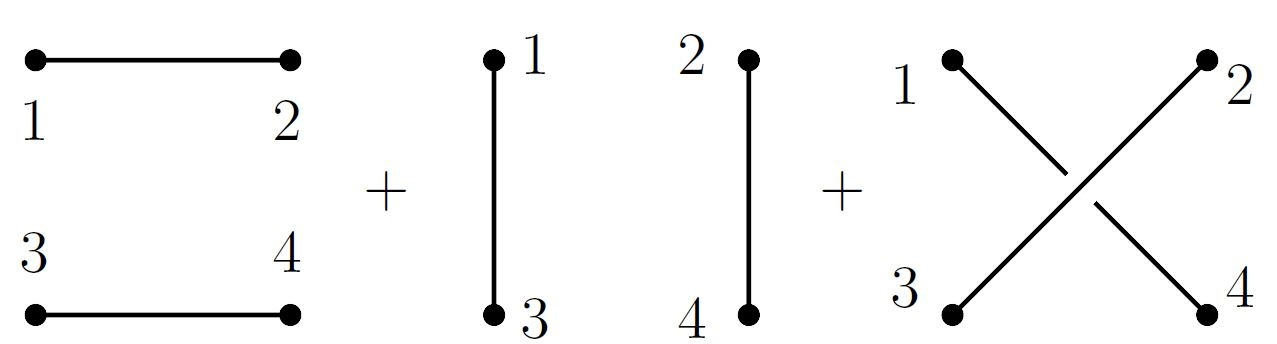
\includegraphics[width=5 cm]{pic/feof4.jpg}\end{aligned};\label{green}
\end{align}
���һ�����Dz�����ͼ�α�ʾ, ������ͼ����. ����, �ھ���Ӧ��ά�˶�������Ҫע��, ���ڷ��������, �����ÿ����һ��Ҫ����һ������.

\subsubsection{��~$\phi^4$ ���۵Ĺ�������Ϊ��: ��ͨͼ, ȫ��ͨͼ; ��Чɢ��ͼ: ȫ��ͨ+�ض�; �໥�����µĴ�����: 1PI ͼ, ����; LSZ Լ����ʽ}
~~~~
����, ��ʵ��������~$\phi^4$ ����
\begin{align}
H_I=\int d^3\bm{x}\mathcal{H}=\int d^3\bm{x}\frac{\lambda}{4!}\phi^4
\end{align}
Ϊ��, �������������໥��������µĹ����������׳�ʲô����, ����֮�õ�һЩһ���Ե���Ҫ����. �㼶����, ����������һ�ߵ����ɷ���������. һ��������, �ɵ������Ϊ
\begin{align}
&\langle\Omega|T\phi_H(x)\phi_H(y)|\Omega\rangle^{(1)}_{\textrm{numerator}}\nonumber\\
=&\langle0|T\phi_{(I)}(x)\phi(y)(-i)\int dt\int d^3\bm{z}\frac{\lambda}{4!}\phi(z)\phi(z)\phi(z)\phi(z)|0\rangle\nonumber\\
=&3\cdot\frac{-i\lambda}{4!}D_F(x-y)\int d^4zD_F(z-z)D_F(z-z)\nonumber\\
&+12\cdot\frac{-i\lambda}{4!}\int d^4zD_F(x-z)D_F(y-z)D_F(z-z)\nonumber\\
=&3\begin{aligned}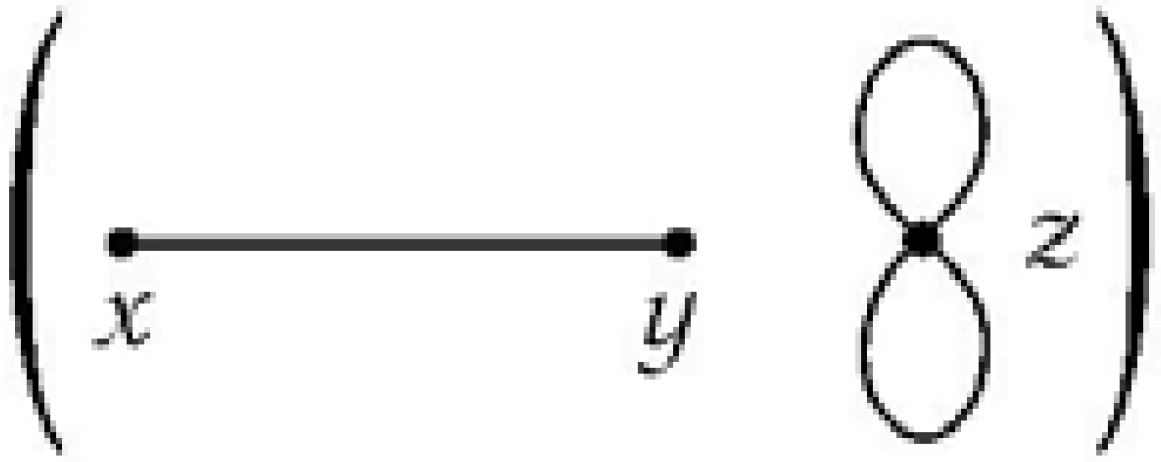
\includegraphics[width=2 cm]{pic/c1.jpg}\end{aligned}+12\begin{aligned}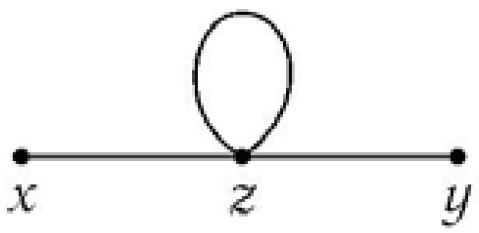
\includegraphics[width=1.8 cm]{pic/c2.jpg}\end{aligned};
\end{align}
��������������ǰѽ���ʽ�����˷���ͼ, ���������~(�����Ϊ~$\phi^4$ ���۵�λ�ÿռ�ķ�������), �Dz���������.

���dz����е㶼�������ߵ�ͼΪ��ͨͼ; �е�δ�������ߵ�ͼΪ����ͨͼ; �պϳ�Ȧ��û�����ߵ�ͼ, �����ͼ. ����ͼΪ��, ��һͼ��Ϊһ����ͨͼ, ����һ����������һ�����ͼ����; �����ڶ�ͼ��Ϊһ��ͨͼ, �˴��ֽ����ͼ. ��չ���������ѿ���, �������������ϵķ���ͨ����, ǡ������ϵ����ͼ��ȫ����. --��ʵ��һ���, ���ͼ�����ͨͼ�Դ�������û�й���. --����, �����������������Ϊ��, ����
\begin{align}
\langle\Omega|T\phi_H(x)\phi_H(y)|\Omega\rangle:=&\begin{aligned}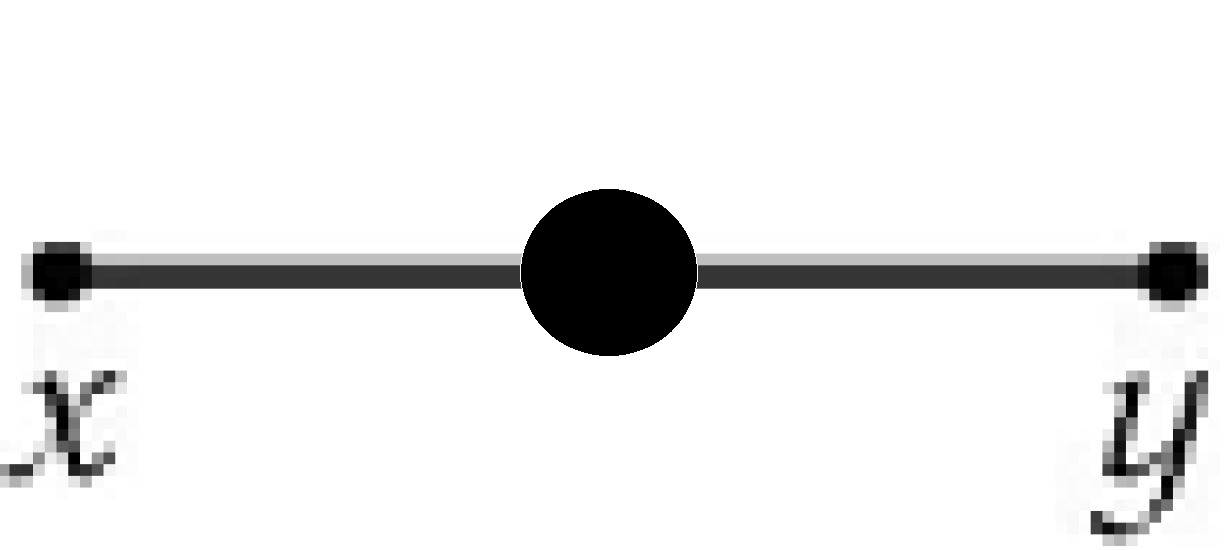
\includegraphics[width=1.3 cm]{pic/pop.jpg}\end{aligned}
=\begin{aligned}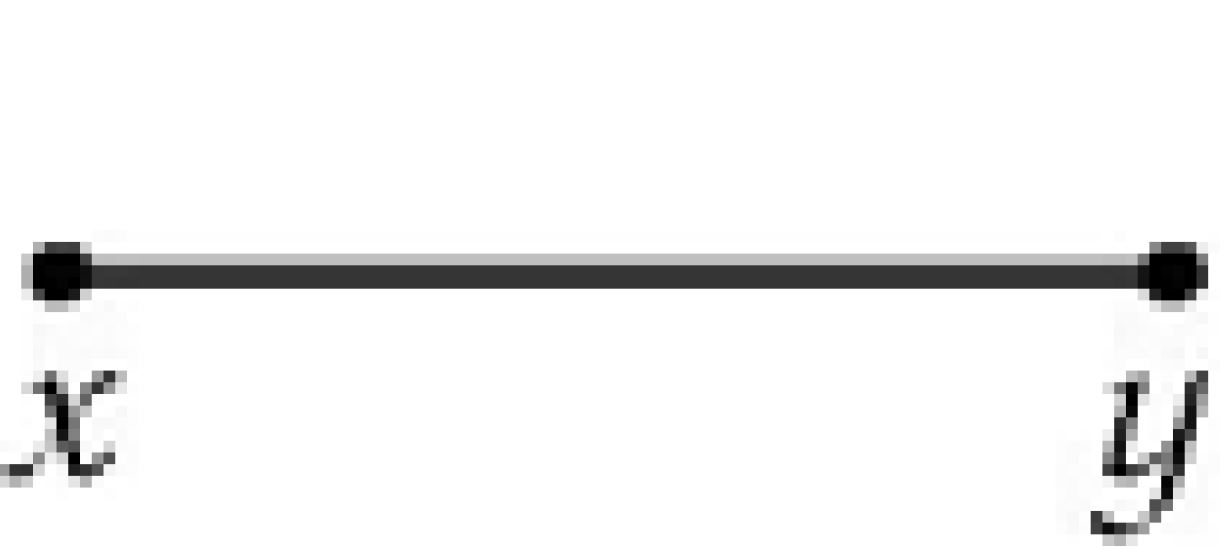
\includegraphics[width=1.3 cm]{pic/pp.jpg}\end{aligned}+12\begin{aligned}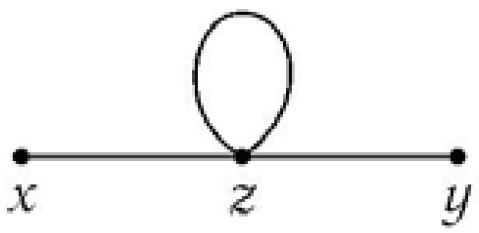
\includegraphics[width=1.6 cm]{pic/c2.jpg}\end{aligned}+\cdots\nonumber\\
=&\textrm{all connected diagrams with two external points}.
\end{align}
���Ƶ�, $n$ ����ֺ������Ǿ���~$n$ ������������ͨͼ; ע����Ҫ���ǵ��Գ�ϵ��. ��Ȼ, ���ڱ�~$\phi^4$ ���, ��������ֺ�����Ϊ���.

����, ����ֻҪ����ͨͼ�ͶԴ��������й���, ����, ��������ĸ��ֺ���, ����~(\ref{green}) ��������ͨͼ, ȴ��ɢ����̵���׽���~(�����²�����׽���, ��ֻҪ���������Ƿ����), ����ζ������������ͨ��, �������ɢ����~(�������ɢ�����; �Ժ����ǽ��о�) ��û�й��׵�. ���, ������������, ����Щ����������ȫ������ͼ, ��ȫ��ͨͼ. ֻ��ȫ��ͨͼ, ��ɢ����̲��й���. ����, �ڶ��ڶ�����ֺ����������, ����������������ͼ, ��Թ�ɢ������޹���~(�������ཫ���Ժ��ʾ): ���ǽ����³�������ֻ���ǽض�ͼ. �Զ���֮, ����ɢ�����~(��ɢ�����), ֻ��ȫ��ͨͼ��ض�ͼ���й���. ����, ~$\phi^4$ ���۵��ĵ���ֺ���, ��һ�׽������й��׵��
\begin{align}\label{four green}
4!\cdot\frac{-i\lambda}{4!}\int d^4zD_F(x_1-z)D_F(x_2-z)D_F(x_3-z)D_F(x_4-z)=\begin{aligned}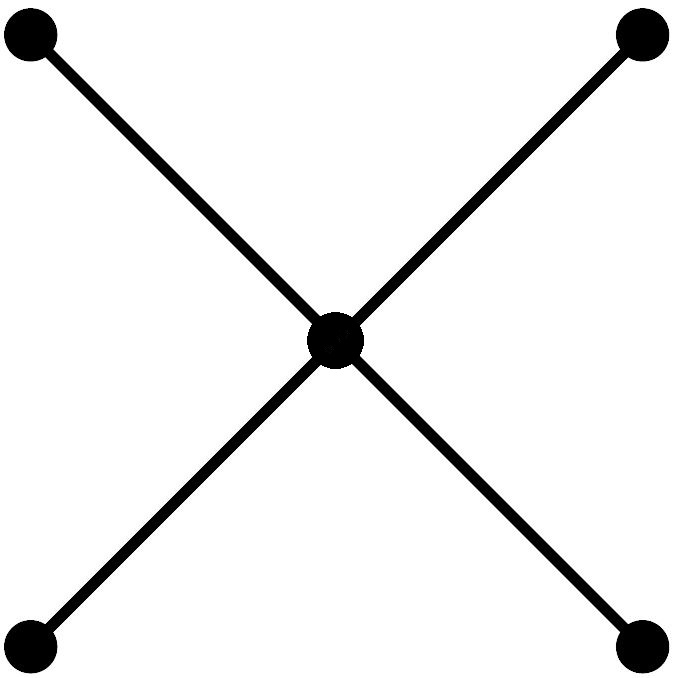
\includegraphics[width=1.2 cm]{pic/phi44.jpg}\end{aligned}.
\end{align}
���������ĶԳ�����~$4!$ �����������еij���~$1/4!$ ����, ��ʵ���������ǽ�����������ѡ���ԭ������.

���, Ӧ��·�����ַ������Է����֤��, $n$ ����ͨ���ֺ����ķ�������, �������ɽϵͽ�ȫ��ͨ�����˻��γɵ�����~$n$ ����ֺ���֮��. ���ǹ���~$Z[J]=e^{iW[J]}$, ����~$iW[J]=\ln Z[J]$; �Ժ�ȷ֤~$iW[J]$ ��ȫ��ͨ���ֺ��������ɷ���:
\begin{align}
G_c(x_1,\cdots,x_n)=\frac{i\delta^nW[J]}{i^n\delta J(x_1)\cdots\delta J(x_n)}\Big|_{J=0}.
\end{align}
����, ���ĵ���ֺ���Ϊ��, ����һ�¼���~$G_c=G(1234)-G(12)G(34)-G(13)G(24)-G(14)G(23)$.







��ǰ���й�����������������ͼ�ķ���, ���ǿ���ζ��������ֺ����ƺ���ij��������; ��ʵ��, �������漴������, �����໥���������, �����������е��������, ������ֺ���֮���ֻ����������~(�ľ�����) �ഩ��һ�����Ѷ���~(�⽫�������ܵĸ���). �������Ǿ����о�����.
%
%�������Ǽ�������һ���໥������, ������������������; ���Ƿ���֮ǰ�ᵽ��������ֺ����Ĵ�������.
%
~���е��κ�һ���߶��޷���������ֵ�ͼ, �е����Ӳ���Լ~(1PI) ͼ, ��~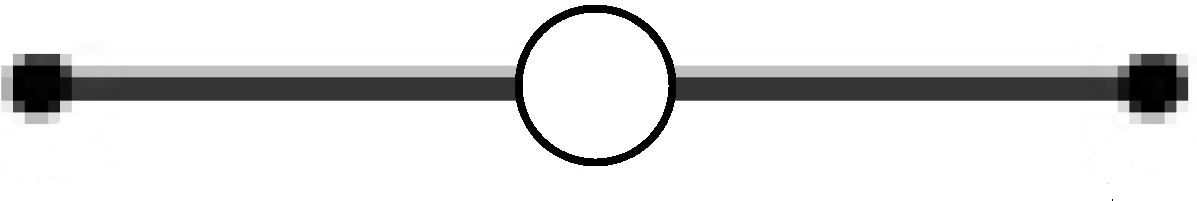
\includegraphics[width=1.1 cm]{pic/1p.jpg} ��ʾ; ���еĿ���Ȧ�������໥�����ܳ�Ϊ����, ��~$-i\Sigma$ ��ʾ. �ɴ˿�֪
\begin{align}
G=&~\begin{aligned}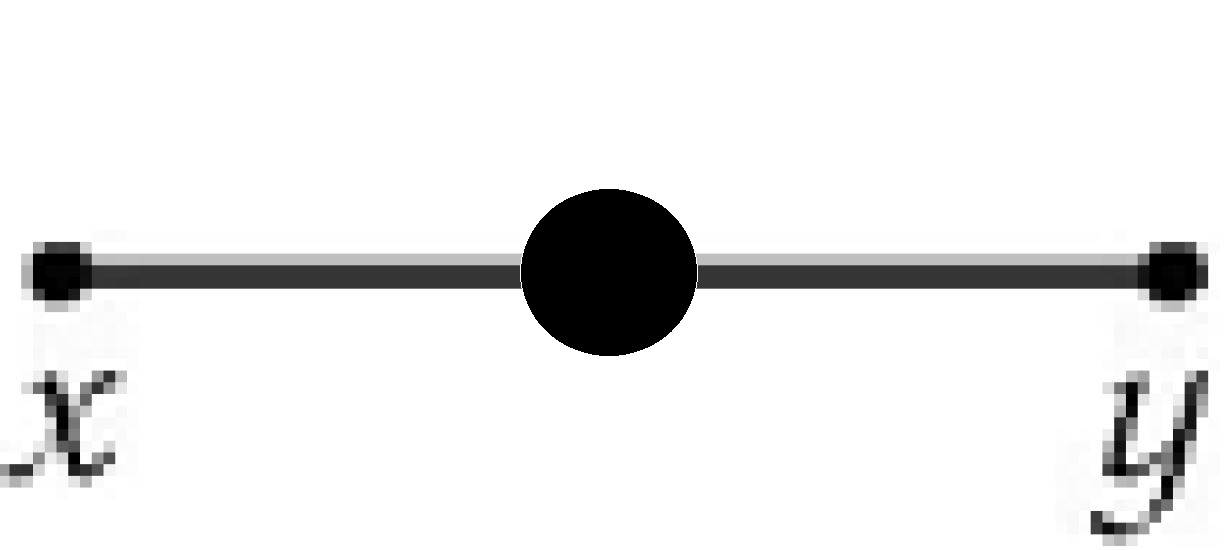
\includegraphics[width=1.3 cm]{pic/pop.jpg}\end{aligned}=\begin{aligned}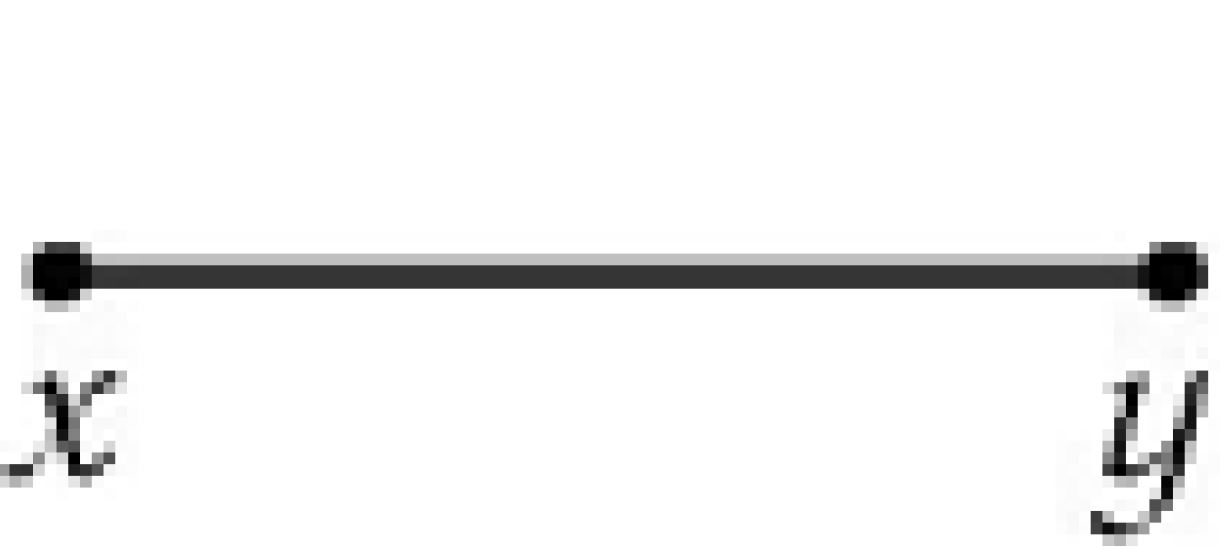
\includegraphics[width=1.3 cm]{pic/pp.jpg}\end{aligned}+\begin{aligned}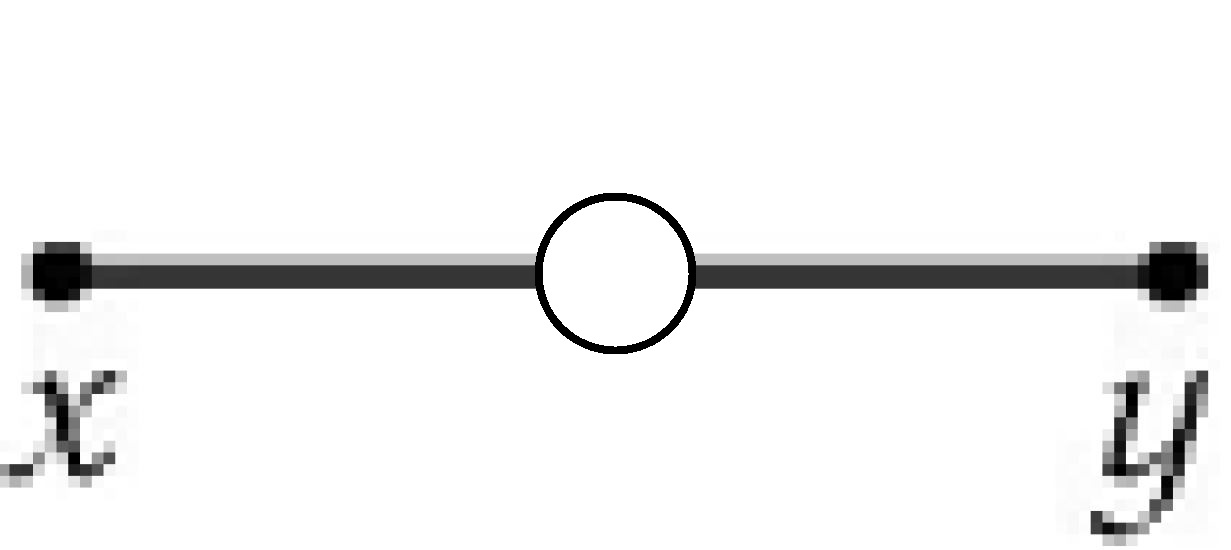
\includegraphics[width=1.3 cm]{pic/1pi.jpg}\end{aligned}
+\begin{aligned}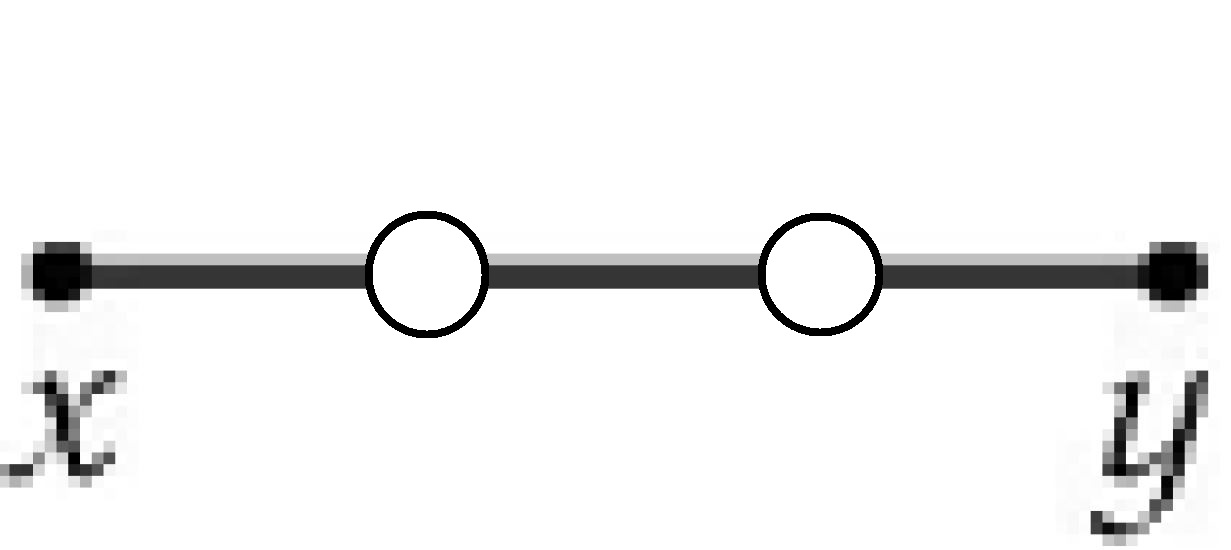
\includegraphics[width=1.3 cm]{pic/1pii.jpg}\end{aligned}+\cdots\nonumber\\
=&G_0+G_0(-i\Sigma)G_0+G_0(-i\Sigma)G_0(-i\Sigma)G_0+\cdots\nonumber\\
=&G_0-iG_0\Sigma G=G_0-iG\Sigma G_0\nonumber\\
=&\frac{G_0}{1+i\Sigma G_0}=(G^{-1}_0+i\Sigma)^{-1}.
\end{align}
������ڱ�����, ������~$G_0=\frac{i}{p^2-m^2+i\epsilon}$, ����~$\phi^4$ �໥�����������ʽ����
\begin{align}
G(p)=\frac{i}{p^2-[m^2+\Sigma(p)]+i\epsilon}:=\frac{i}{p^2-m_c^2+i\epsilon}.
\end{align}
Ҳ����˵, $\Sigma(p)$ �������໥���ö���������������; ���������ǽ����Ϊ���ܵ�ԭ��. �����, ���ǵ�����, �ɳ�Ϊ��������~$\phi^4$ ������µ�����; �Ժ����ǻ����о�����������������, ����~QED �е�����. ����, ǰ�ĵ����ͼ, ��ν�DZ�������������ܵ�һ������. ��Ȼ��������±�����ֻ��һ������; ������Ժ󽫷��ֵĵ��ӿɾ��и߽�����.






��С�����, �������о�~LSZ Լ����ʽ. ���Ա�����Ϊ��, �ڵ�һ���������ѵõ�, ����������۲����~$a_L^\dag:=\sqrt{2E_{\bm{p}}}a^\dag_{\bm{p}}=-\int d^3\bm{x}e^{-ipx}i\overset{\leftrightarrow}{\partial}_0\phi(x)$~(ע������~$e^{-ipx}=\langle x|p\rangle$ ������۲���ĵ�����̬); �������ǿɵ�
\begin{align}
a_L^\dag(+\infty)-a_L^\dag(-\infty)=&\int_{-\infty}^{+\infty}dt \partial_0a_L^\dag\nonumber\\
=&-\int d^4x e^{-ipx}i(\partial^2+m^2)\phi(x).
\end{align}
����֪��, ɢ�������Ա�Ϊ~$\langle0|\cdots a_L(+\infty)\cdots a^\dag_L(-\infty)\cdots|0\rangle$, �ɴ����Ǽ��ɵõ�
\begin{align}
\langle f|S|i\rangle=&\prod_{i,j=1}^{n,n'}\int dx_idx'_je^{-ip_ix_i}e^{ip'_jx'_j}i(\partial^2_i+m)i(\partial^2_j+m)\nonumber\\
&~~~~~~~~~~~~~~~~~~~~~~~~~~\cdot \langle\Omega|T\phi_{(I)}(x'_1)\cdots \phi(x'_{n'})\phi(x_1)\cdots\phi(x_n)|\Omega\rangle;
\end{align}
������������Ȼ��һ����ĩ̬����~$n,~n'$ �����ӵ�ɢ�����, ��ɢ�������~$(n+n')$ ����ֺ���֮��Ĺ�ϵ, ��Ϊ~LSZ Լ����ʽ. ֱ�������, ����һ���໥���ù��̵ķ���ͼ����, ϵ�����ú��ϵ�, �����߶δ�����, ��ͼ��͸������ֺ���; ������������, �͸���ɢ�����. ��ʽ�ұ�, ����ζ�Ž�ϵ�����ú��ϵ����ɴ�����, ��������̬. ��ʵ��, �����ӳ��۵�·�����ַ�����, ��ʽ���Ǽ���ɢ�����Ļ�����ʽ; ��ʱ�÷���������~$S$ ����, �����ҵ��ľ������ʽ��. �����Ƶ�����, ���Ǿ��ݲ�������.
%LSZ ��׳���.

\subsubsection{$\phi^4$ ���۵�ɢ����������ͼ}
~~~~
����, ��~$\phi^4$ �����Ϊ��, ������չʾһ��ɢ������ķ���ͼ��������ֺ���ͼ������, ˳��չʾһ��~LSZ ����. ǰ����, �����ѵõ�������µ��ĵ���ֺ���, ����, ����Ҫ������ӳ�~(����۲���) ̬������~$|i\rangle=|p_1p_2\rangle=\sqrt{4E_{\bm{p}_1}E_{\bm{p}_2}}a_1^\dag a_2^\dag |0\rangle$ ��ĩ������~$|f\rangle=|p_3p_4\rangle=\sqrt{4E_{\bm{p}_3}E_{\bm{p}_4}}{a}_3^\dag {a}_4^\dag |0\rangle$ ��ɢ�����. ����׽��Ƽ�
\begin{align}
S_{fi}^{(0)}=&\langle p_3p_4|p_1p_2\rangle=\langle p_3|p_1\rangle\langle p_4|p_2\rangle+\langle p_3|p_2\rangle\langle p_4|p_1\rangle\nonumber\\
=&(2\pi)^8\delta^4(p_3-p_1)\delta^4(p_4-p_2)+(2\pi)^8\delta^4(p_3-p_2)\delta^4(p_4-p_1)\nonumber\\
%=&4\sqrt{E_{\bm{p}_1}E_{\bm{p}_2}E_{\bm{p}_3}E_{\bm{p}_4}}\langle0|a_3a_4a^\dag_1a^\dag_2   |0\rangle\nonumber\\
%=&4E_{\bm{p}_1}E_{\bm{p}_2}(2\pi)^6\delta^3(\bm{p}_1-\bm{p}_3)\delta^3(\bm{p}_2-\bm{p}_4)+\delta^3(\bm{p}_2-\bm{p}_3)\delta^3(\bm{p}_1-\bm{p}_4)\nonumber\\
=&\begin{aligned}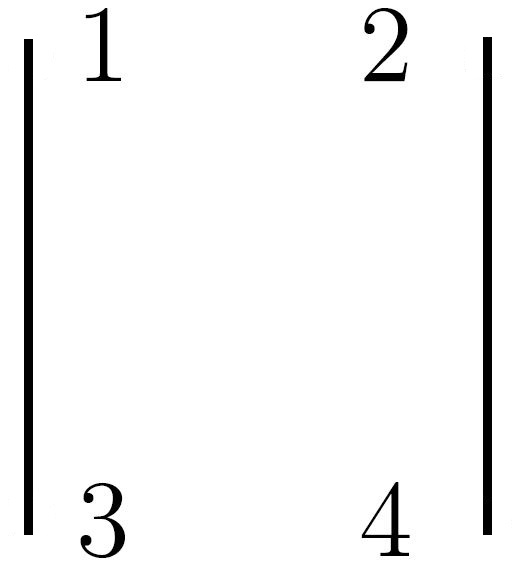
\includegraphics[width=1.1 cm]{pic/a1.jpg}\end{aligned}+\begin{aligned}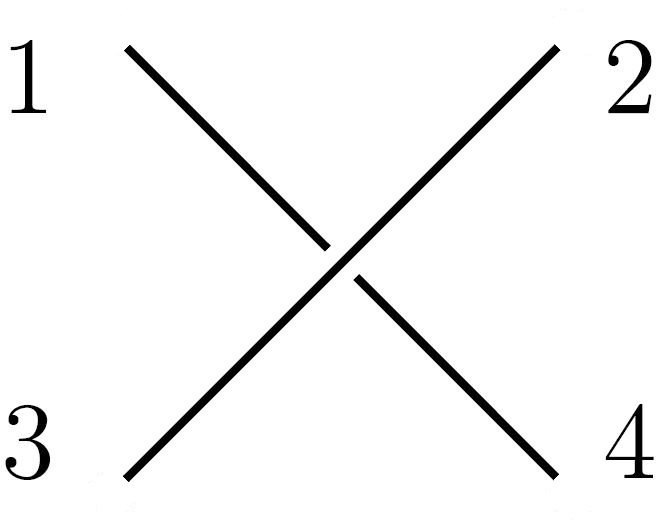
\includegraphics[width=1.7 cm]{pic/a2.jpg}\end{aligned}.
\end{align}
ֵ��ע��: ���ֺ�������ͼ��������, ��ʾ���Ӵ�λ�ÿռ�ij�㵽��һ��Ĵ���~(��Ȼ����Ҫ���϶�λ�õ���ά����); ɢ���������ͼ�е�������, ��ʾ����֮��Ĵ���. ��ɢ����̵�һ�׽�����
\begin{align}
&-i\frac{\lambda}{4!}\langle p_3p_4|\int dx^4T\phi^4(x)|p_1p_2\rangle\nonumber\\
=&-i\frac{\lambda}{4!}\langle p_3p_4|\int dx^4\left(:\phi\phi\phi\phi:+6\contraction[0.6ex]{}{\phi}{}{\phi}\phi\phi :\phi\phi:+3\contraction[0.6ex]{}{\phi}{}{\phi}\phi\phi\contraction[0.6ex]{}{\phi}{}{\phi}\phi\phi \right)|p_1p_2\rangle
\end{align}
���е�������ǰ�ĵ����������߳����������, ��~$\begin{aligned}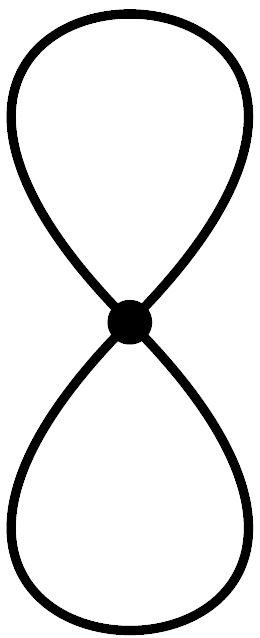
\includegraphics[width=0.4 cm]{pic/loop.jpg}\end{aligned}\times \left(\begin{aligned}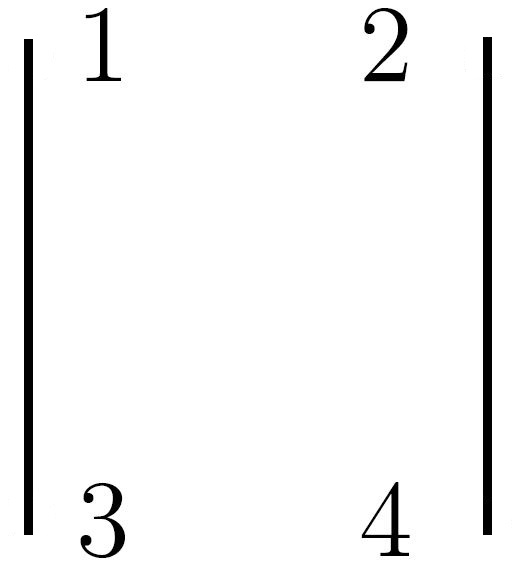
\includegraphics[width=1.1 cm]{pic/a1.jpg}\end{aligned}+\begin{aligned}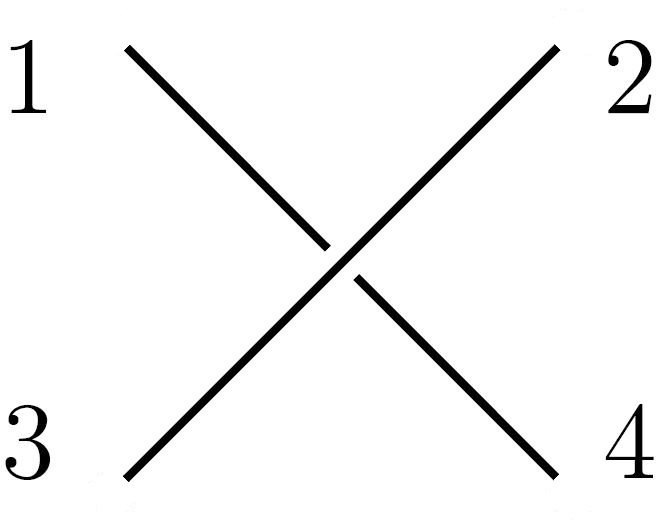
\includegraphics[width=1.3 cm]{pic/a2.jpg}\end{aligned}\right)$, ����δ������ײ, �ʶ�һ�����Ϊ��. �ڶ���Ϊһ�����ɴ����߳���һ�����ͼ, ��~$\begin{aligned}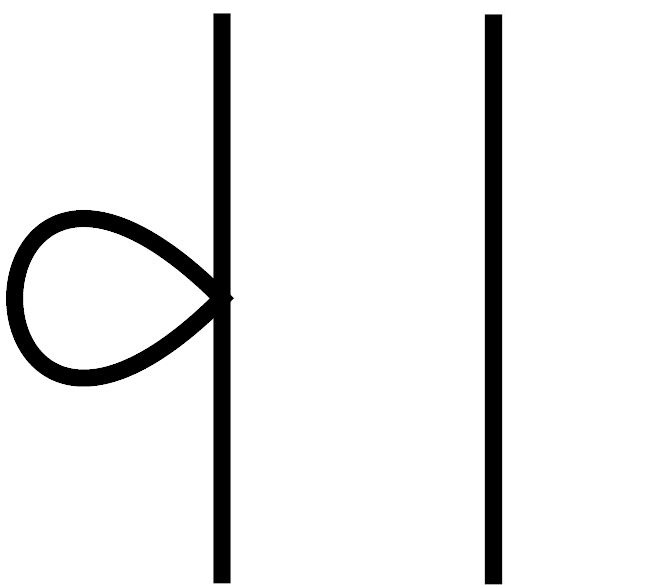
\includegraphics[width=1.1 cm]{pic/kedou.jpg}\end{aligned}$; ����~(ͬ�������~$6\times4=24$ ��) ����򽲿�ֵ�ֵΪ
\begin{align}
-i\lambda\int d^4x e^{ip_3x}\int\frac{d^4p}{(2\pi)^4}\frac{i}{p^2-m^2}e^{-ip_1x}=-i\lambda\delta^4(p_3-p_1)\int\frac{d^4p}{(2\pi)^4}\frac{i}{p^2-m^2}.
\end{align}
�ɼ���������ʽ��, ����Ķ����غ�ʹ���ĩ̬��ͬ. �ɴ˿ɼ�, �������͵����ɢ������û�й��׵�; ǰ�ĵ����˵���˴���֤. �������Ƶ���, �����õ���
\begin{align}
\phi|p\rangle=\phi^+|p\rangle=\int\frac{d^3\bm{p}'}{(2\pi)^3\sqrt{2E_{\bm{p}'}}}a_{\bm{p}'}e^{-ip'x}\sqrt{2E_{\bm{p}}}a_{\bm{p}}^\dag|0\rangle=
e^{-ipx}|0\rangle.
\end{align}
���, ǰ��һ�׽��Ƶĵ�һ�����
\begin{align}
4!\cdot\frac{-i\lambda}{4!}\int d^4xe^{-i(p_1+p_2-p_3-p_4)x}=&-i\lambda(2\pi)^4\delta^4(p_1+p_2-p_3-p_4)\nonumber\\
=&\begin{aligned}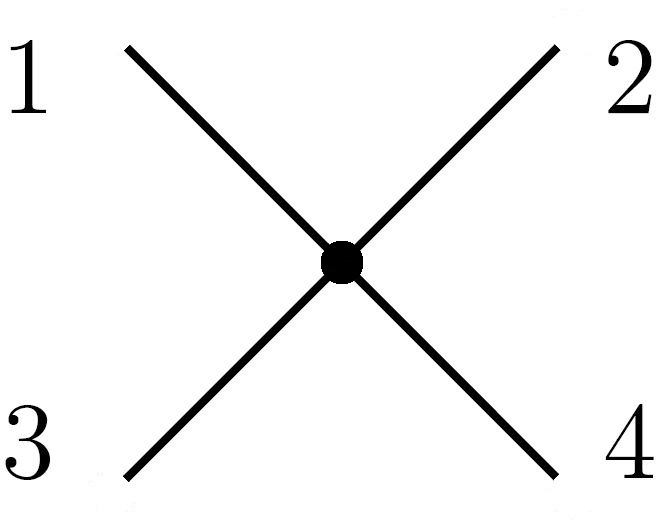
\includegraphics[width=1.7 cm]{pic/aaa.jpg}\end{aligned},
\end{align}
�˼�~$\phi^4$ �����ж�ɢ������й��׵�һ����. ĩ��, ��Ϊ����˵��������Ӷ�������~$\delta$ �����������߽������µ������, ����Ҳ�����׷��ֵ�������������������, ��~$\begin{aligned}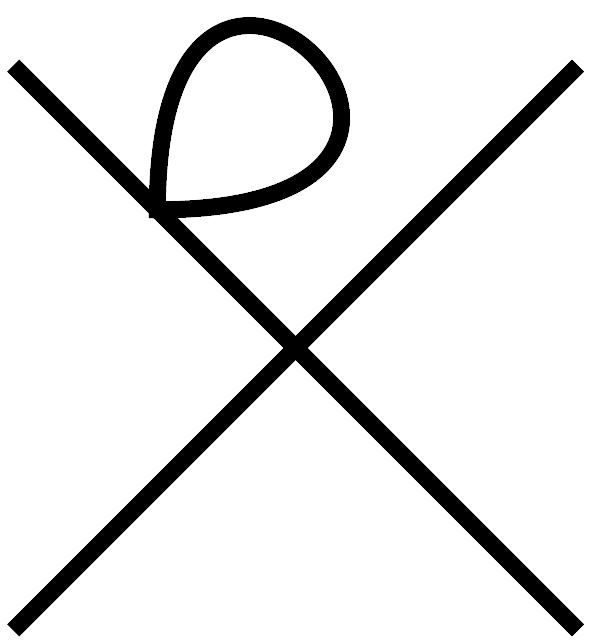
\includegraphics[width=1.1 cm]{pic/leg.jpg}\end{aligned}$ ��, ��ɢ��������޹��׵�. ǰ�������ἰ, �˴���֤.


�Ա���ǰ���ĵ��������ʽ~(\ref{four green}), ����ؼ�
\begin{align}
G(34,12)=-i\lambda\int d^4zD_F(x_3-z)D_F(x_4-z)D_F(z-x_1)D_F(z-x_2),
\end{align}
���Լ���, $\phi^4$ �����е��ĵ���ֺ���, �����е���Ӧ��������ɢ�����, ǡ��~LSZ ��ʽ��ϵ����. �Ƶ���ע���õ�ʽ~(\ref{green f}).

$\phi^4$ ����¶�����ɢ���һ�׽���, ���˷�����ȫ. �Ա�ǰ��ɢ�����Ԫ����ʽ, �ҵ��ó�ʱ���̵�ɢ�����Ϊ~$\mathcal{M}=-\lambda$. ���ɺ��ļ������ֵ�ɢ�����ı���ʽ, ���ǿ��Եó��˹��̵ķ�΢����Ϊ
\begin{align}
\left(\frac{d\sigma}{d\Omega}\right)_{\textrm{CM}}=\frac{\lambda^2}{64\pi^2E^2_{\textrm{cm}}},
\end{align}
�����ܽ���~$\sigma=\frac{\lambda^2}{32\pi E_{\textrm{cm}}}$. ʵ����, ����˴���ɢ�����, ���ɵó������۵����ǿ��~$\lambda$.

��С�ڵ�֪ʶ��, ������ṹ�����, �������໥������ʽ���dz�����; �Ժ��ڲ�ͬ�ij�������Ӧ�����, ���ǻ����������������ʽ. �����һ��, ������, ���Ƕ�����д������ʽ, �ٻ�������ͼ��. �Ժ�, ���ǽ�����ᵽһ�����̵�ij�׽���~(����˵������ײ�������ӵ�ɢ��Ķ��׽���), �����ͼ���Ƚ���ʽ����ֱ�۹�����. ��ʱ, һ���, ���Ƕ����Ȼ�������ͼ, ������Ӧ�ķ�������д�������ʽ. ���ѳ����ֽ��ۼ����е���������֮һ.




\subsubsection{˥�����, ɢ�����}


~~~~����֪��, ��������ʵ����, ��Ϊ������ֱ�ӹ۲��, һ�����˥����Ȼ�ɢ������; ����������������ĵĻ���Ƶ������Ķ���ѧ��, ��ɢ�����. ��ô, ��ɢ�����˥����Ȼ�ɢ���������ô������������? �������Ǿ������������֮��.

\paragraph{˥�����}
~

˥�����~$\Gamma$~(���������ĵ���) ������һ��ʱ��~$T$ �ڵ�ԾǨ����~$P$, ��~$\Gamma\propto\frac{P}{T}$. �����ֻ̬��һ������, ��ĩ̬�����ж������, ��ӳ�̬��ĩ̬��Ծ���ʾ���~$P=\frac{|S_{fi}|^2}{\langle i|i\rangle\langle f|f\rangle}$. ����ĩ̬�Ĺ�һ��Ϊ~$\langle i|i\rangle=(2\pi)^32E_{\bm{p}_I}\delta^3(0):=2E_{\bm{p}_I}V,~\langle f|f\rangle=\prod_f2E_{\bm{p}_f}V$. �����������ʼ���Ӵ��ھ�ֹ״̬, ��~$E_{\bm{p}_I}=m$, �������ǿɵ�
\begin{align}
P=\frac{|\mathcal{M}_{fi}|^2}{2mV}(2\pi)^4\delta^4(p_I-p_F)VT\prod_f\frac{1}{2E_{\bm{p}_f}V};
\end{align}
����������ȡ~$(2\pi)^4\delta^4(0)=VT$. ������
\begin{gather}
d\Gamma:=\frac{P}{T}=\frac{|\mathcal{M}_{fi}|^2}{2m}(2\pi)^4\delta^4(p_I-p_F)\prod_f\frac{d^3\bm{p}_f}{(2\pi)^3}\frac{1}{2E_{\bm{p}_f}}:=\frac{|\mathcal{M}_{fi}|^2}{2m}d\Pi,\\
\Gamma=\sum_f\int\frac{|\mathcal{M}_{fi}|^2}{2m}d\Pi;
\end{gather}
%����~$d\Pi$ Ϊ����۲��������ռ�΢Ԫ.
����
\begin{gather}
\int d\Pi=\int(2\pi)^4\delta^4(p_I-p_F)\prod_f\frac{d^3\bm{p}_f}{(2\pi)^3}\frac{1}{2E_{\bm{p}_f}}
\end{gather}
Ϊ����۲��������ռ�.

\paragraph{ɢ�����}
~

���ϼ�˥�������ɢ�����֮��Ĺ�ϵ; ����, �����ҳ�ɢ�����~$\sigma$ ��ɢ�����֮��Ĺ�ϵ. Ϊ��, ����Ҫ����Ҫ�ҵ���ײ����~$(d\Gamma)_{\textrm{two~initial~states}}$ ��ɢ�����֮��Ĺ�ϵ.

�������������Ϊ~$A$ ��Ŀ��������ƽ�������������. ����������~$N_T$ ����, ÿ���е���Ч���--�˼�ɢ�����--Ϊ~$\sigma$, ��ô, �����������ӵ�~(��) ɢ�����, �༴����һ����ײ�¼��ĸ��ʾ���
\begin{align}
probability=\frac{N_T\sigma}{A}=\frac{events}{N_B};
\end{align}
����~$events$ Ϊ��ײ�¼���, $N_B$ Ϊ������������. �ɴ����ǿ��Լ����
\begin{align}
\sigma=\frac{events}{N_BN_T}A=\frac{events}{(\rho vtA)N_T}A=\frac{events/(N_T t)}{\rho v}:=\frac{events/(N_T t)}{j}
\end{align}
ʵ����, ���ƺ�������~$j$ ��, ���~$n_T:=events/(N_T t)$ ���ɶ���ɢ�����. ��������, ����
\begin{align}
d\sigma=&\frac{(d\Gamma)_{\textrm{two~initial~states}}}{j}=\frac{(d\Gamma)_{\textrm{two~initial~states}}}{\rho|\bm{v}_1-\bm{v}_2|}\nonumber\\
=&\frac{1}{4E_1E_2V}|\mathcal{M}_{fi}|^2d\Pi\cdot\frac{V}{|\bm{v}_1-\bm{v}_2|}\nonumber\\
=&\frac{1}{4E_1E_2}\frac{1}{|\bm{v}_1-\bm{v}_2|}|\mathcal{M}_{fi}|^2d\Pi=\frac{1}{4|\bm{p}_1E_2-\bm{p}_2E_1|}|\mathcal{M}_{fi}|^2d\Pi\nonumber\\
=&\frac{1}{4\sqrt{(p_1p_2)^2-m_1^2m_2^2}}|\mathcal{M}_{fi}|^2d\Pi
\end{align}
�����õ���~$\bm{p}=E\bm{v}$. �����ܻ���ʱ, ע��Լ�����������̬ƽ��ĩ̬���, �Լ������ظ�����.

����, ����ĩ̬���������ӵ����, ���ǽ�����һ������һ����. ��ĩ̬���������ӱ��Ϊ~$a,~b$, ������������ϵ, ������
\begin{align}
&\int d\Pi_2=\int\frac{d\Omega |\bm{p}_a|^2d|\bm{p}_a|}{(2\pi)^34E_aE_b}(2\pi)\delta(E_{\textrm{cm}}-E_a-E_b)\nonumber\\
=&\int d\Omega\frac{|\bm{p}_a|^2}{16\pi^2E_aE_b}\left(\frac{|\bm{p}_a|}{E_a}+\frac{|\bm{p}_a|}{E_b}\right)^{-1}=\int d\Omega\frac{|\bm{p}_a|}{16\pi^2E_{\textrm{cm}}},
\end{align}
�����õ���~$\int dx\delta(g(x))=\sum_i\frac{1}{|g'(x_i)|}$; ���ǿɵ�
\begin{align}
\left(\frac{d\sigma}{d\Omega}\right)_{\textrm{CM}}=\frac{1}{4|\bm{p}_1E_2-\bm{p}_2E_1|}\frac{|\bm{p}_a|}{16\pi^2E_{\textrm{cm}}}|\mathcal{M}_{fi}|^2.
\end{align}
����ĩ̬~4 ������������ͬ, �����ǻ��ɽ�һ���õ�
\begin{align}
\left(\frac{d\sigma}{d\Omega}\right)_{\textrm{CM}}=\frac{|\mathcal{M}|^2}{64\pi^2E^2_{\textrm{cm}}}.
\end{align}

\subsection{Yukawa~����}
%ע��, ����۲����̬����֮ǰ������~$|p^\mu>$, ����
\subsubsection{�Լ�������Ϊ��: ɢ������������ͼ���������, ��ͼ~(��������������), Ȧͼ~(���������)}
\paragraph{һ�����ӵ���������˥��: $\pi-NN$ }
~

Ϊ��������˵�������, �ڱ��ڼ��Ժ�ĸ���������, ���Ƕ��Ȳ��������������������, Ȼ���ٽ���һ�������������ʾ; ���ȿ��DZ���~Yukawa ����, �ٿ�������~Yukawa ����.

����һ�����ӵ��������ӵ�˥��~$\pi-NN$. ��˽�����ά����Ϊ~$\bm{p}$, ��������۲��������̬��~$|p\rangle=\sqrt{2E_{\bm{p}}}|\bm{p}\rangle=\sqrt{2E_{\bm{p}}}a^\dag_{\bm{p}}|0\rangle$; �˼���̬~$|i\rangle$. ����������Ӷ����ֱ�Ϊ~$\bm{p}'_1,~\bm{p}'_2$, ����ĩ̬��~$|f\rangle=\sqrt{4E_{\bm{p}'_2}E_{\bm{p}'_2}}b^\dag_{\bm{p}'_1}c^\dag_{\bm{p}'_2}|0\rangle$. ����,  Yukawa~�����, �˹���ɢ�����Ԫһ�׽��ƾ���
\begin{align}
\langle f|S|i\rangle^{(1)}=&-ig\langle f|T\int d^4x\psi^\dag(x)\psi(x)\phi(x)|i\rangle\nonumber\\
=&-ig(2\pi)^4\delta^4(p'_1+p'_2-p)\nonumber\\
=&\begin{aligned}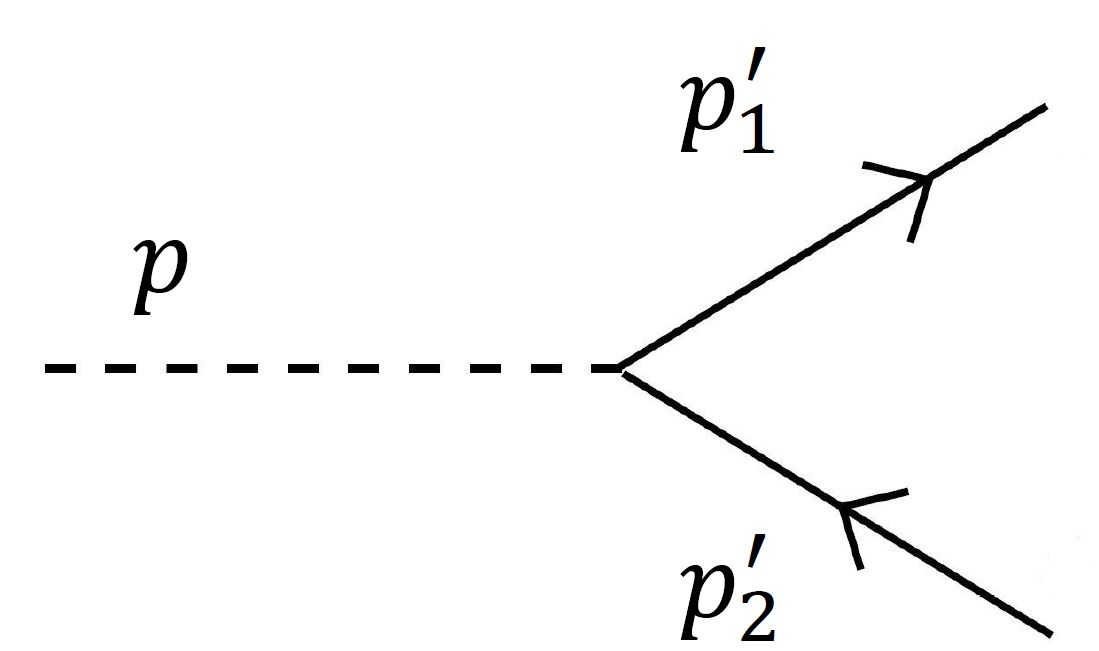
\includegraphics[width=2.4 cm]{pic/meson.jpg}\end{aligned};
\end{align}
�������ǵõ��˹��̵�ɢ�������~$\mathcal{M}=-g$. ����������, ���������Ƚ��н�������, ��󻭳��˹��̵�~(�����ռ��) ����ͼ; �����~(�����, �˴���~Yukawa ���۶����ռ�ķ�������), ���ǿ��������, ���綥��Ҫ������ά�����غ�~(���������غ�����ά�����غ�) ���ӵȵ�. ֵ��ע�����, �����ϵļ�ͷ, �������ӵ��˶�����, ���Ǵ�����ɵ�����. һ���, ���㴦����Ҫ�������غ��. �������ǰ����������ӵ��������ǽ���, --���ཫʹ���ǻ�÷����ӵķ���ͼ/��������. ���Ѽ����
\begin{align}
\psi|p,s\rangle=&\psi^+|p,s\rangle=\int\frac{d^3\bm{p}'}{(2\pi)^3\sqrt{2E_{\bm{p}'}}}a^{s'}_{\bm{p}'}u^{s'}(p')e^{-ip'x}\sqrt{2E_{\bm{p}}}a_{\bm{p}}^{s\dag}|0\rangle\nonumber\\
=&u^s(p)e^{-ipx}|0\rangle,
\end{align}
�ɴ����ǿɵñ�������
\begin{align}
\langle f|S|i\rangle^{(1)}=&-ig\bar{u}^{s}(p'_1)v^{r}(p'_2)(2\pi)^4\delta^4(p'_1+p'_2-p)\nonumber\\
=&\begin{aligned}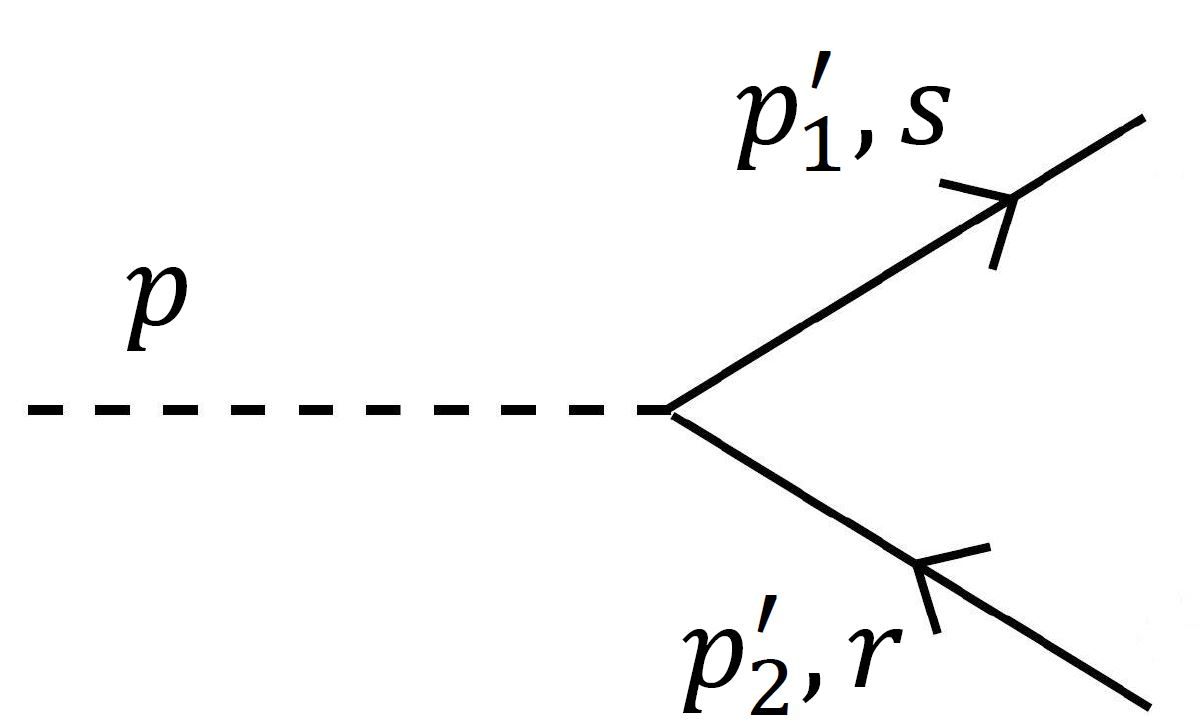
\includegraphics[width=2.4 cm]{pic/meson2.jpg}\end{aligned}.
\end{align}
������������Զ���, ��Ҫ�ֱ��ٸ���~$\bar{u}^{s'}(q_1)$ ��~$v^{r'}(q_2)$, ����dz��߷����ӵķ�������.


\paragraph{�������ӵ�ɢ��: $NN-NN$}
~

�������ǿ����������ӵ�ɢ��~$NN-NN$. ���Կ���, �˹��̵�ɢ�����Ԫһ�׽�����, ����Ƕ��׵�. ����һ������, ���ǵ�
\begin{align}
S^{(2)}_{fi}&=i(-ig)^2\left[\frac{1}{(p_1-p'_1)^2-m^2}+\frac{1}{(p_1-p'_2)^2-m^2}\right](2\pi)^4\delta^4(p_1+p_2-p'_1-p'_2)\nonumber\\
&=\begin{aligned}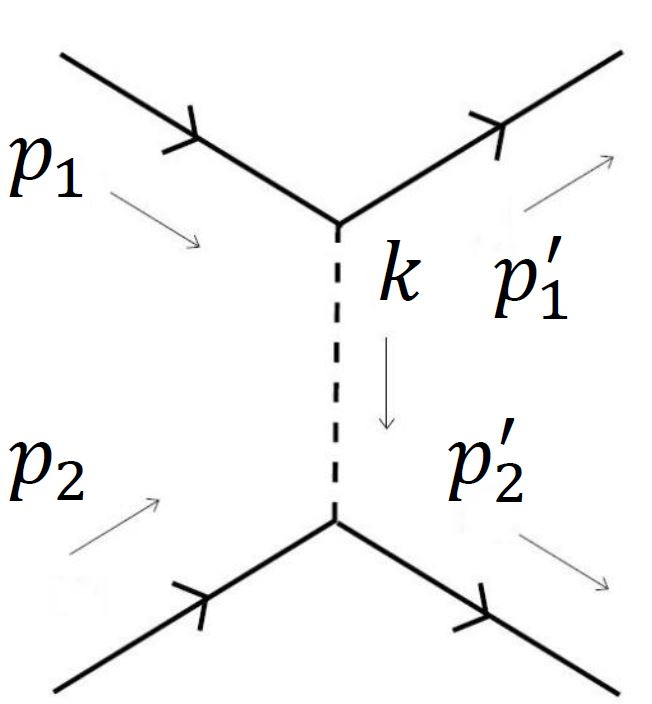
\includegraphics[width=1.7 cm]{pic/nn-nn.jpg}\end{aligned}+\begin{aligned}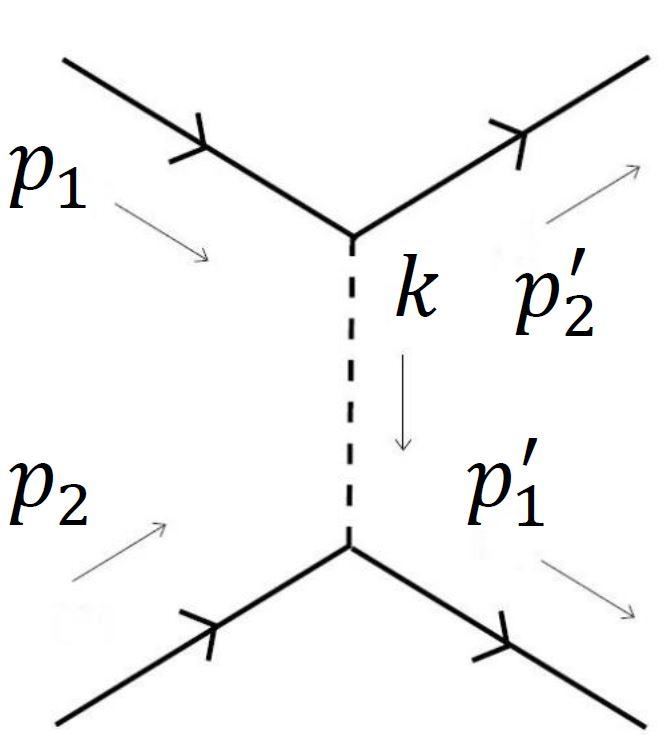
\includegraphics[width=1.7 cm]{pic/nn-nn2.jpg}\end{aligned}.\label{two n}
\end{align}
��ʽ���������ķ��������Dz�����ᵽ��: ������Ӧ��һ��������. ��Ȼ, ��Ҫע��˴����Ӳ������ʿ�����, ����ǵ�; ����������/�����Ӷ�Ӧ���Dz���̽��������.

��ʽ��ʾ������ͼ��, ��Ϊ��ͼ; ���Ǹ��߽�΢��, ���ǽ��õ���Ȧ��ͼ, ��ΪȦͼ. ��һ��������˵��, ɢ���������������ֻ��ȫ��ͨͼ��ض�ͼ; Ҳ����˵Ȧ�������ϵ�ͼ��������, �������ϵ�, ��~$\begin{aligned}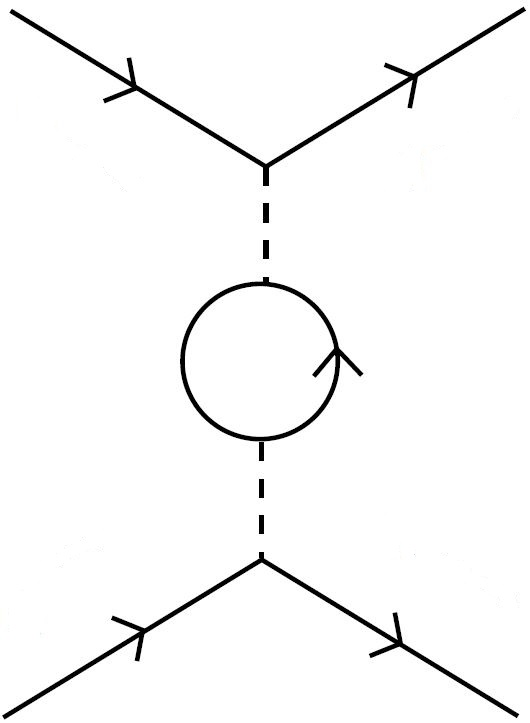
\includegraphics[width=1.2 cm]{pic/vp.jpg}\end{aligned}$ ���й���~(�������ǹ���, ��������ϵ�Ȧ����������ռ���/��������, �����ǰ�ĵ��ӵ�����). ����, ��������ͼ����ӵ�, ����ϵ����ĩ̬�����ӽ���������������; �����Dz�ɫ��ϵ������~(��Ȼ��Ҳ��������ע�⵽, �Ժ�����ӵ�ɢ�����������, ��ĩ̬�����ӽ���Ҫ����һ������).

����, ��ʽ�е�һͼ��Ϊ~$t$-channel; �ڶ�ͼ, �ڷ�������������ó��߽���~(����һͼʽ), ��Ϊ~$u$-channel.


��Ȼ, �ɷ���ͼ, ������ɲ��ؾ����ȶ���ɢ�����Ԫ���õ�ɢ�����, ������ֱ�Ӵ�ͼ����ɢ�����~$\mathcal{M}$. ��Ȼ, ��ͼ��Ӧ��ɢ�����, ���������Ӧ�ķ�������; ����֮�Ƿdz����׵�.

����, ���Ǿ������Ǽ������������, ����ȥ�����غ�Ȳ���, ֱ���ó�ɢ�����. ��ʱ�ɼ����
\begin{align}
\mathcal{M}^{(2)}_{fi}&=(-ig)^2\left[\frac{\bar{u}^{s'}(p'_1)u^s(p_1)\bar{u}^{r'}(p'_2)u^r(p_2)}{(p_1-p'_1)^2-m^2}
-\frac{\bar{u}^{r'}(p'_2)u^s(p_1)\bar{u}^{s'}(p'_1)u^r(p_2)}{(p_1-p'_2)^2-m^2}\right]\nonumber\\
&=\begin{aligned}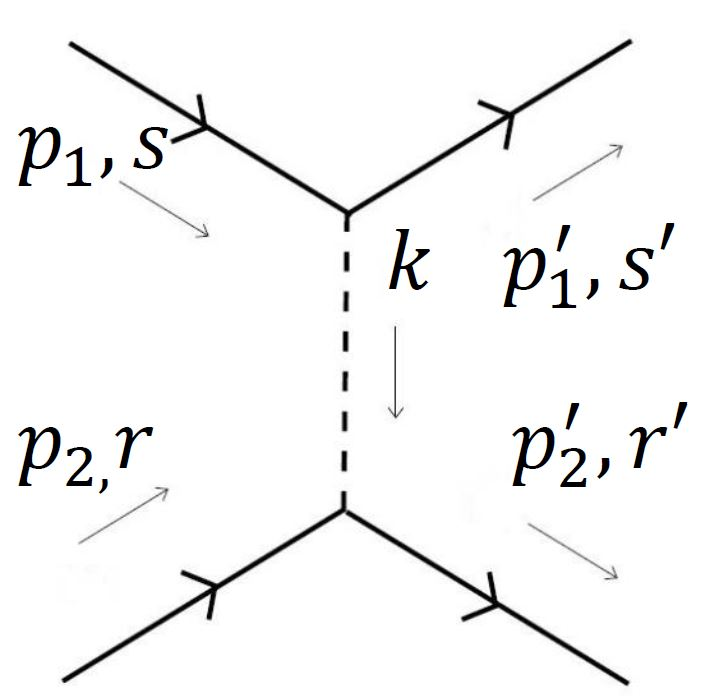
\includegraphics[width=1.9 cm]{pic/nn-nna.jpg}\end{aligned}+\begin{aligned}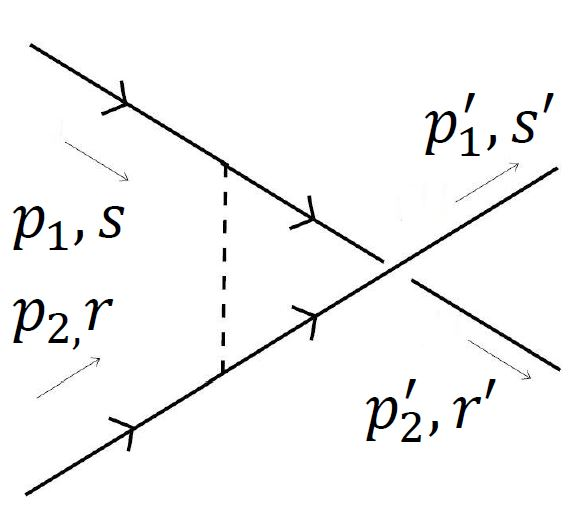
\includegraphics[width=2.0 cm]{pic/nn-nnb.jpg}\end{aligned}.\label{two n}
\end{align}
����ͼ-ʽ֮��ķ�������, ���Dz���������; ����ĩ�߽�����ָ�����������һ������, �ȵ�.

��֮, ���������ļ���, ����ʹ�Լ����ȷ����, ����ͼ����������ȷ�ǵȼ۵�. ����, ����������ǰһ��˵����, �Ժ�����һ�㲻�ٽ���ɢ�����/�������ԭʼλ�ÿռ䳡����ʽ���������ռ����ļ���, ��ֱ�Ӵ���ȷ�����ķ���ͼ�������.



%��Ȼ, �������������, ��, ����˵, ���Ӳ�һ�������. �����ڴ��������ײ, �������; ������Ϊ��������ײ������, �������.

%������̬�ϵ�����, ����? ɢ�䲻����ֺ���, �������ǻ�̬, �����������ȫ����; ɢ��, ��������������Ҳû��, Ϊʲô, �����ĩ̬������ѽ, ����������̬������, bingo!
%���ֺ������, �໥��������Լ���ȫ����, ֯�����õ����; ɢ��������, Ҳ������.

\paragraph{�����������ӵ�ɢ��: $N\bar{N}-N\bar{N}$}
~

�������ǿ��Ǻ���-�����ӵ�ɢ��~$N\bar{N}-N\bar{N}$; ����ֱ�Ӵ�ͼд��ɢ������Ľ���ʽ:
\begin{align}
i\mathcal{M}^{(2)}=&\begin{aligned}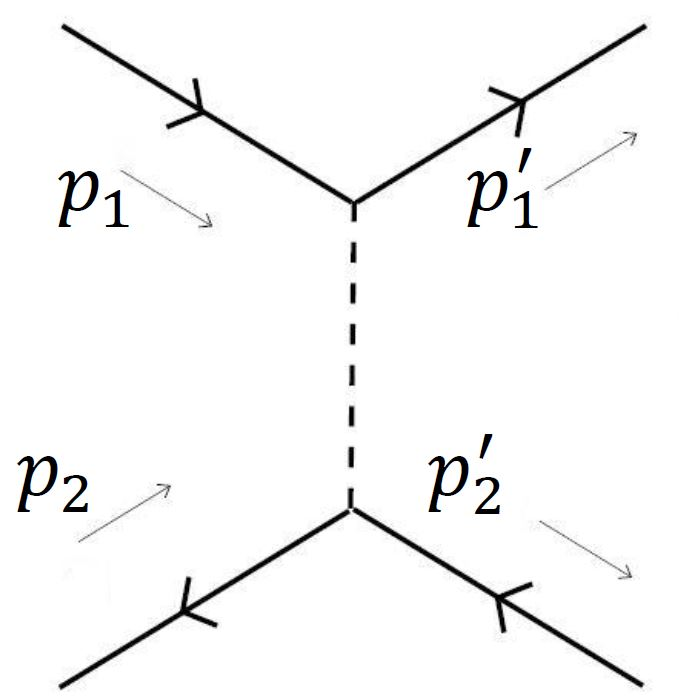
\includegraphics[width=1.8 cm]{pic/nn-1.jpg}\end{aligned}+\begin{aligned}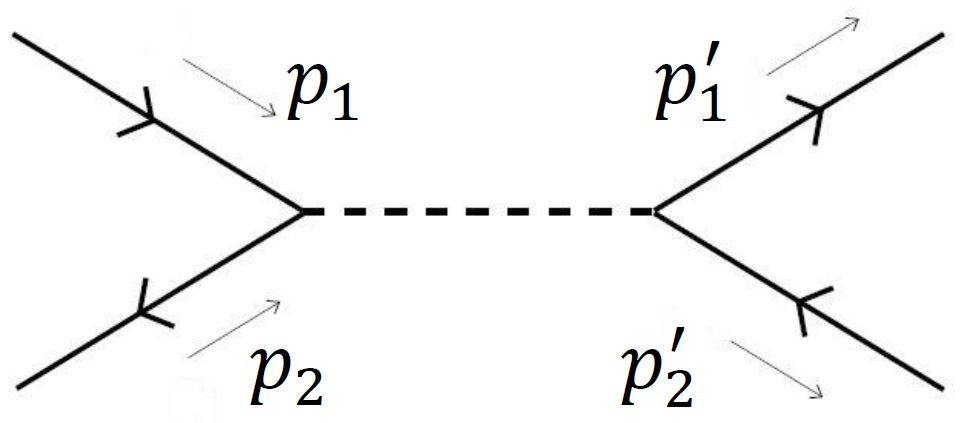
\includegraphics[width=2.6 cm]{pic/nn-2.jpg}\end{aligned}\nonumber\\
=&i(-ig)^2\left[\frac{1}{(p_1-p'_1)^2-m^2}+\frac{1}{(p_1+p_2)^2-m^2+i\epsilon}\right].
\end{align}
�ɴ˿ɼ�, ��Ϊ��ɵ�ԭ��, ���dz�����һ���µ�ͼ��, ������Ϊ~$s$-channel �������ڶ�ͼ. ������ϵ��, ��ͼ�ķ�ĸ��д��Ϊ~$4(M^2+\bm{p}^2)-m^2$; �ɴ���Ȼ��֪, s channel �е���������, δ����������ǵ�, Ҳ�������ڿ�����; �ڿ�ʱɢ�����������һ�������ֵ. ��ʵ��, ����~$Z^0_\mu$ ��ɫ�ӵ�, ���Ǿ����������ֵ�.

����������, ��ɢ����׹��̾�Ϊ
\begin{align}
i\mathcal{M}^{(2)}=&\begin{aligned}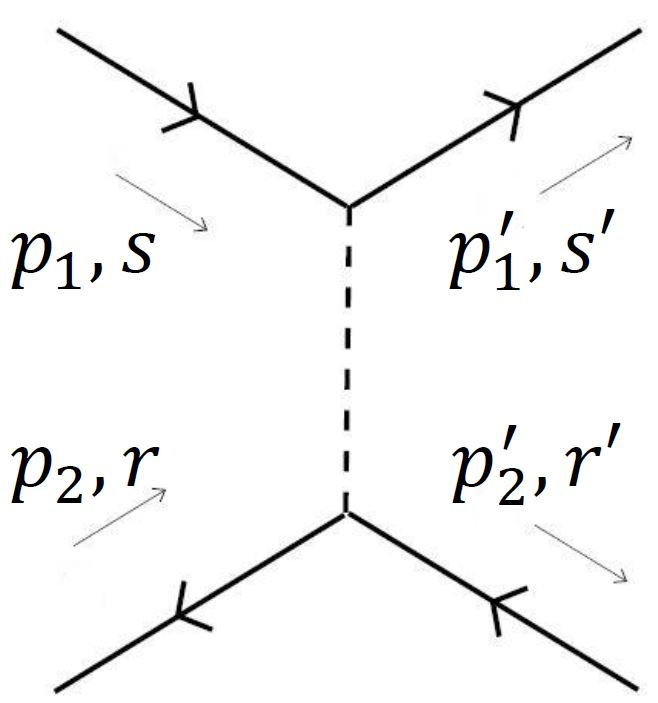
\includegraphics[width=1.8 cm]{pic/nn-a.jpg}\end{aligned}+\begin{aligned}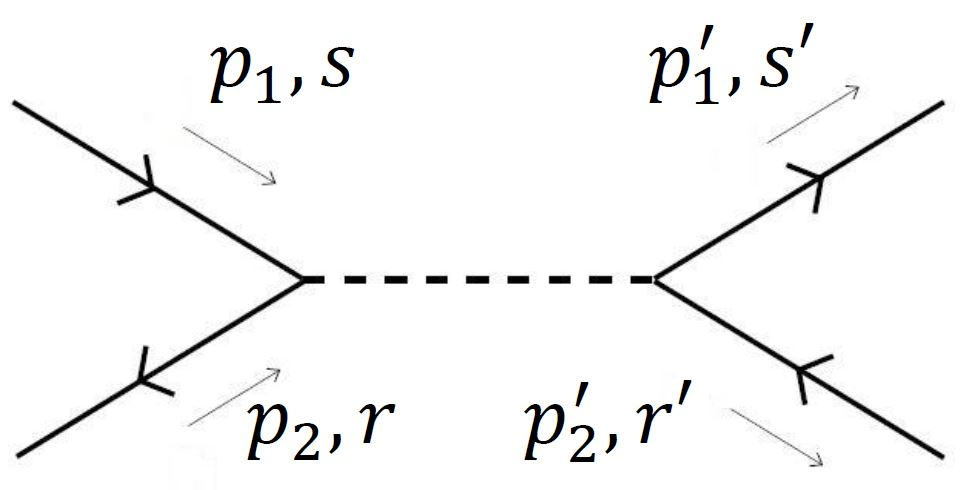
\includegraphics[width=2.6 cm]{pic/nn-b.jpg}\end{aligned}\nonumber\\
=&i(-ig)^2\left[\frac{\bar{u}^{s'}(p'_1)u^s(p_1)v^{r'}(p'_2)\bar{v}^r(p_2)}{(p_1-p'_1)^2-m^2}+\frac{\bar{v}^r(p_2)u^s(p_1)\bar{u}^{s'}(p'_1)v^{r'}(p'_2)}{(p_1+p_2)^2-m^2+i\epsilon}\right].
\end{align}






\subsubsection{����Գ���, $s/t/u$-channel, Mandelstam ����}
~~~~
�ڶ�ʽ�Ļ��, ���Կ������ڵ�һʽ��������
\begin{align}
p'_2\rightarrow-p_2,~p_2\rightarrow-p'_2
\end{align}
�Ľ��. Ҳ����˵, һ�˰���һ���ض����������ӵĹ��̵����, ������һ�˰���һ�������෴�����ķ����ӵĹ��̵����. ��, ��Ϊ����Գ���.




��һС���������Ѽ�����ͼ��~$s/t/u$-channel ֮�ֱ�. ����������~channel, ���Ƿֱ���䳣�ö������Ϊ
\begin{align}
s=(p_1+p_2)^2=(p'_1+p'_2)^2,\\
t=(p_1-p'_1)^2=(p_2-p'_2)^2,\\
u=(p_1-p'_2)^2=(p_2-p'_1)^2;
\end{align}
��Ϊ~Mandelstam ����. ��Ȼ�����ĸ��������غ��, ��~$p_1+p_2=p'_1+p'_2$; ��Ҳ����˵��������~Mandelstam �����Dz�������. ���������о�����. ��~$\theta$ ��������������ߵļн�; ��~$E_{\textrm{CM}}$ ������ϵ�¶���������~(��ά�����غ��ʱ������������غ�), ����Ϊ��������ȡ�������������, ��~$E_{\textrm{CM}}=2E$); ����, ����������ϵ��, ���Ǿ���~$p_1=(E,0,0,\bm{p}),~p_2=(E,0,0,-\bm{p}),~p'_1=(E,0,\bm{p}\sin\theta,\bm{p}\cos\theta),~p'_2=(E,0,-\bm{p}\sin\theta,-\bm{p}\cos\theta)$; ��һ���ɵ�~$s=4E^2=E_{\textrm{CM}}^2,~t=-2\bm{p}^2(1-\cos\theta),~u=-2\bm{p}^2(1+\cos\theta)$~(�ɴ˿�֪~$\theta=0$ ʱ~$t$ ���̲��������ȫ����~$u$ ����; $\theta=\pi$ ʱ~$u$ ���̲�����, ���ȫ����~$t$ ����; ��Ȼһ�������, ��������������̵ĺ�). ����, ���Ǿ͵õ�~$s+t+u=4E^2-4\bm{p}^2=4m^2$. �����ĸ�������������ȵ����; ��������������ʱ, ����
\begin{align}
s+t+u=\sum_i m_i^2
\end{align}

%���ӳ�����������ѧ�IJ��, ������һά���άг����, �Ӷ��ȼ۵��������ڹ����, ����Ҫ��, ���ǶԴ���ν����, �༴���Ŀ����IJ�ͬ��.


\subsubsection{Yukawa~��}
~~~~
�ھ�����ѧ��������ѧ��������, �����Ӽ�͸���м����ӵ��໥����, ����Ϊ�����Ӽ�����ν�໥������; �����ڵ����µ���Ч����. ����, ���Ǿ�������~Yukawa ����ڵ����µ���Ч��, ��~Yukawa ��. ������~$NN-NN$ ɢ��Ϊ��, ����������ϵ��, �˹��̵�ɢ�����~(\ref{two n}) ����дΪ
\begin{align}
i\mathcal{M}^{(2)}=+ig^2\left[\frac{1}{(\bm{p}-\bm{p}')^2+m^2}+\frac{1}{(\bm{p}+\bm{p}')^2+m^2}\right];
\end{align}
ǰ������ֱ����������Ӵ�����̬~$|\bm{p}\rangle$ ��~$|\bm{p}'\rangle$ ��~$|-\bm{p}'\rangle$ ��ԾǨ. ���ǿ��ǵ�һ��, �������Ӵ�~$|\bm{p}\rangle$ ��~$|\bm{p}'\rangle$ �Ĺ���. �ڵ���/������ѧ������, ���ǰ�����һ�����ӵĴ��ڿ���һ���Ƴ�~$U(\bm{r})$; ���������µ�һ������ɢ�����, �ڵ��ܽ��ƺ�, ����Ϊ��һ�������ڴ���֮�е�ɢ�����. ����, ������������ѧ����ֱ�������Ӧ��������������ĵ��ܽ��~(��ʱǰ�ĵõ���ɢ�����Ԫʽ������Ч��): ��ȷ�������Ч��, ����~$-i\langle\bm{p}'|U(\bm{r})|\bm{p}\rangle=-i\int d^3\bm{r}U(\bm{r})e^{-i(\bm{p}-\bm{p}')\cdot\bm{r}}$; ����ʽ����ʽ�е�һ�����, �͵õ�
\begin{align}
\int d^3\bm{r}U(\bm{r})e^{-i(\bm{p}-\bm{p}')\cdot\bm{r}}=\frac{-(\lambda:=g/2M)^2}{(\bm{p}-\bm{p}')^2+m^2};
\end{align}
����ʽ���ɽ��
\begin{align}
U(\bm{r})=&-\lambda^2\int \frac{d^3\bm{p}}{(2\pi)^3}\frac{e^{i\bm{p}\cdot\bm{r}}}{\bm{p}^2+m^2}\nonumber\\
=&-\frac{\lambda^2}{(2\pi)^2}\int_0^{+\infty}\frac{dpp^2}{p^2+m^2} \frac{e^{ipr}-e^{-ipr}}{ipr}\nonumber\\
=&-\frac{\lambda^2}{2\pi r}\int_{-\infty}^{+\infty}\frac{dp}{2\pi i} \frac{pe^{ipr}}{p^2+m^2}\nonumber\\
=&-\frac{\lambda^2}{4\pi r}e^{-mr}.
\end{align}
�˼�~Yukawa ����ڵ����µ�~Yukawa ��. ��ʽ�еĸ��ű�����Ч~Yukawa ��~(����֮��ͨ�����ӵ��໥����) ��������. ����, ��ʽ��~$m$ �Ǹ��ܹ۵������������������м����ӵ�����; �ɼ��м����������뾭�����̴�С�ʷ�������ϵ. ��Ȼ, ����������ɵ����ϵĵ��ܽ��Ƶõ�; �����ǽ��ڵ綯��ѧ�г���. ע����ܹ۵��µ��ӽ������м䲣ɫ�ӹ���������, ���Ӧ�ڵ�����dz�������һ��ʵ.




\subsection{���ӵ綯��ѧ: ���ɢ���������Ķ���~(��ͼ) ����}

~~~~��������~(��һ��ش��������) ����ӵ��໥���õ���������, ��Ϊ���ӵ綯��ѧ. �Ե��������Ϊ��, һ���, ���ǿ���������һЩ���ɢ�����:
\begin{itemize}
\item ���ն�ɢ��/�����ӿ��ն�ɢ��~$e^-+\gamma=e^-+\gamma,~e^++\gamma=e^++\gamma$;
\item ���ӶԲ���/����~$\gamma+\gamma=e^-+e^+,~e^-+e^+=\gamma+\gamma$;
\item ����ɢ��~$e^-+e^-=e^-+e^-$;
\item �Ͱ�ɢ��~$e^-+e^+=e^-+e^+$;
\item ������ɢ��~$e^++e^+=e^++e^+$;
\item ���·���~$e^-+N=e^-+N+\gamma$,
\end{itemize}
�ȵ�.%��Щʽ��, ��������ͼ, �ǰ�����������Ȧͼ�ľ�ȷʾ�����.



��ǰ��~Yukawa �������Ƶ�, ���ǿ��Ƚ��������ij��ɢ����̵�~(�����) ɢ�����, ��ͨ���������������õ���Ӧ���̵�ͼ�λ���ʾ~(����ʱ����ͼ); Ȼ��, ��һ���, ���ǿ��Ȼ�������ͼ, ��ͨ�����������д����Ӧ����ɢ������Ľ�������ʽ. ����, ���Dz���׸��, ��ֱ�Ӹ������ӵ綯��ѧ�ķ�������. ����, ������֪ij���������߶�Ӧ��Ӧ�Ĵ�����, ���������ǹ���ʱ��Ȼ��Ȼ����; �ڶ�, ���߹�������Ҳҵ������, ���������ǹ��ӵ�����, ����һ����Ӧ�ļ���ʸ������; ����, Ҳ��������������, ��������ö���, Ϊ~$-ie\gamma^\mu$.

�ɴ�, ���ǾͿ����ض�����ͼ, д����Ӧ���ɢ�����ɢ������Ķ��׽��ƽ����. ��������ɢ��, �˼�
\begin{align}
&i\mathcal{M}^{(2)}=\begin{aligned}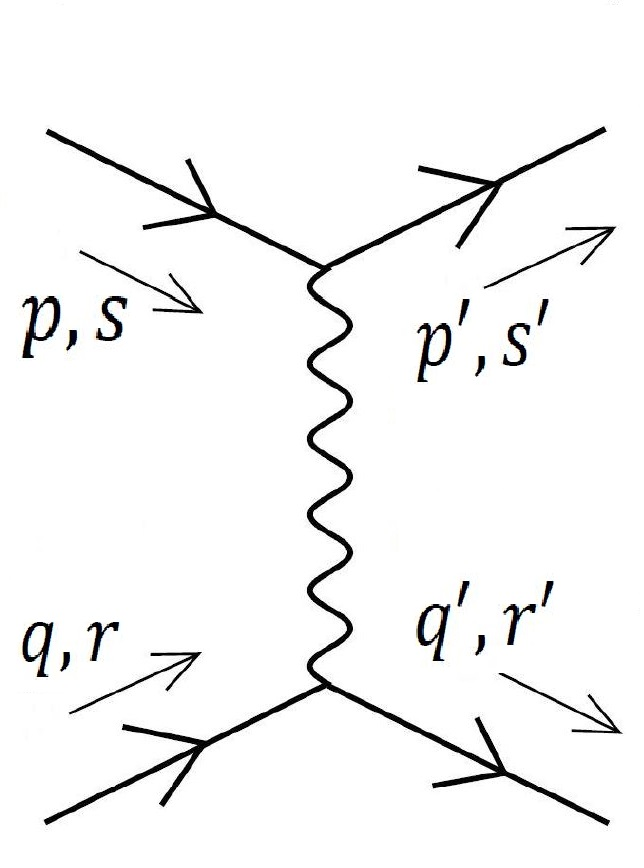
\includegraphics[width=1.7 cm]{pic/ee-ee.jpg}\end{aligned}+\begin{aligned}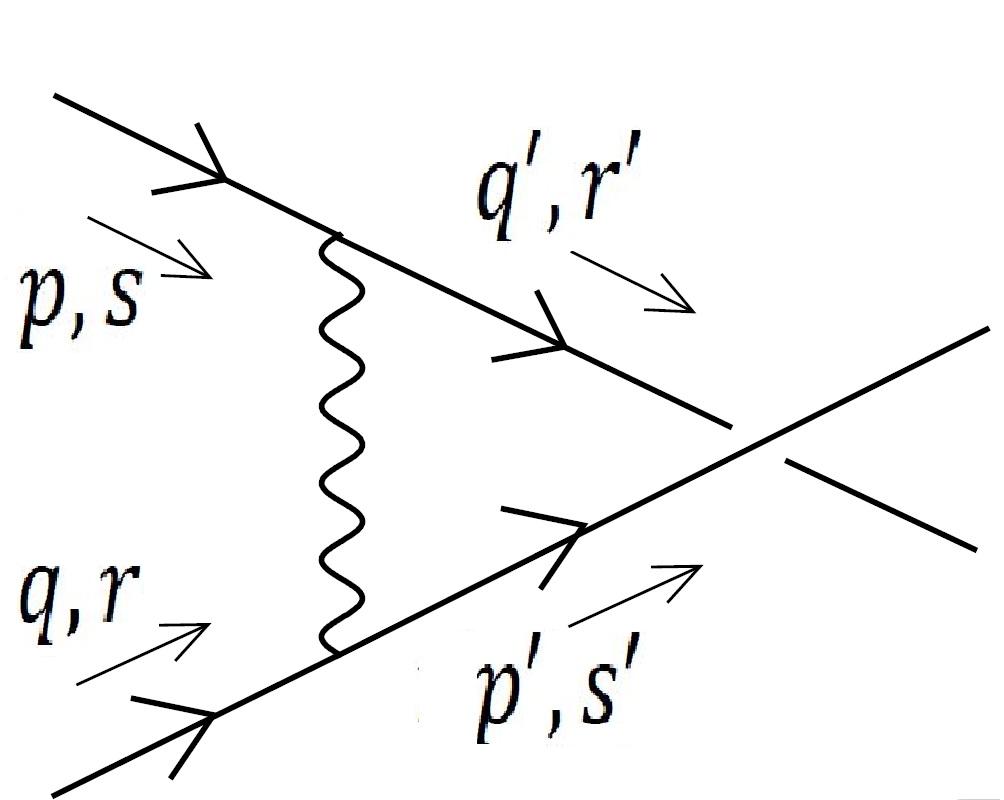
\includegraphics[width=2.1 cm]{pic/ee-ee2.jpg}\end{aligned}\nonumber\\
=&-i(-ie)^2\left[\frac{\bar{u}^{s'}(p')\gamma^\mu u^s(p)\bar{u}^{r'}(q')\gamma_\mu u^r(q)}{(p-p')^2}-\frac{\bar{u}^{r'}(q')\gamma^\mu u^s(p)\bar{u}^{s'}(p')\gamma_\mu u^r(q)}{(p-q')^2}\right].
\end{align}
���ڰͰ�ɢ��, ���ǿɵ�
\begin{align}
&i\mathcal{M}^{(2)}=\begin{aligned}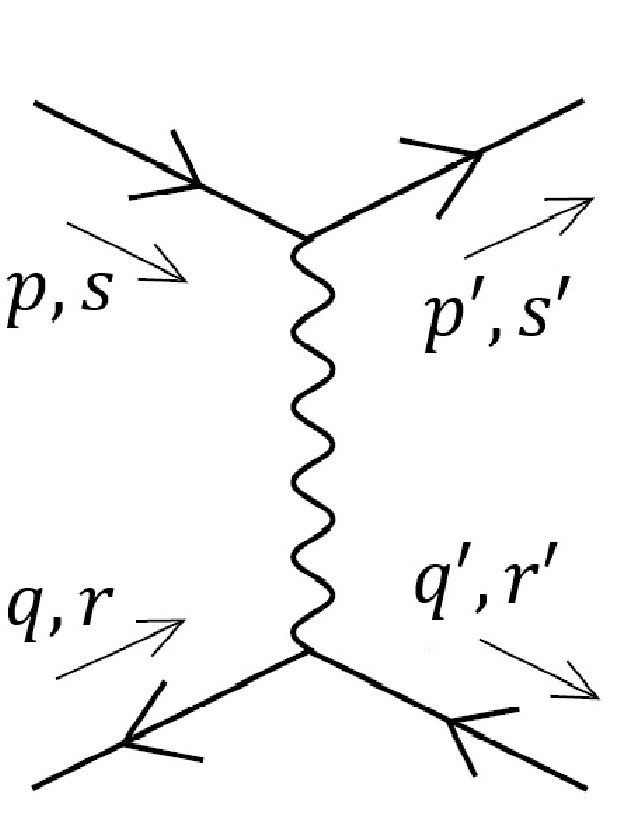
\includegraphics[width=1.7 cm]{pic/bb.jpg}\end{aligned}+\begin{aligned}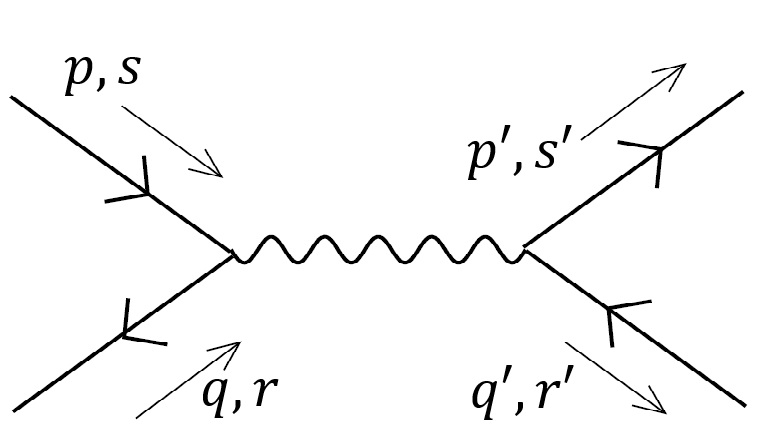
\includegraphics[width=2.7 cm]{pic/bb2.jpg}\end{aligned}\nonumber\\
=&-i(-ie)^2\left[-\frac{\bar{u}^{s'}(p')\gamma^\mu u^s(p)\bar{v}^{r}(q)\gamma_\mu v^{r'}(q')}{(p-p')^2}+\frac{\bar{v}^{r}(q)\gamma^\mu u^s(p)\bar{u}^{s'}(p')\gamma_\mu v^{r'}(q')}{(p+q)^2}\right].
\end{align}
�����������Ӷ�����, ������
\begin{align}
&i\mathcal{M}^{(2)}=\begin{aligned}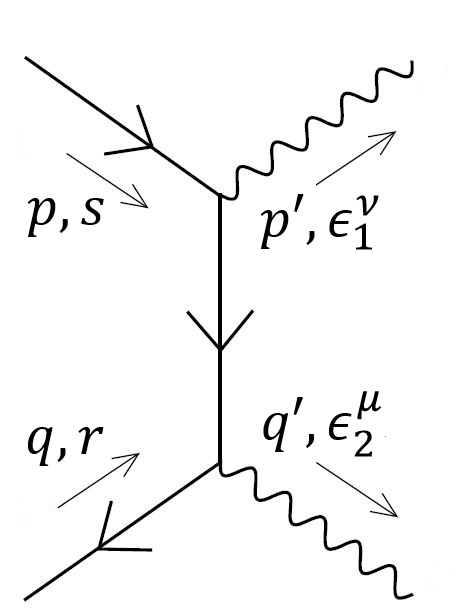
\includegraphics[width=1.8 cm]{pic/eeg.jpg}\end{aligned}+\begin{aligned}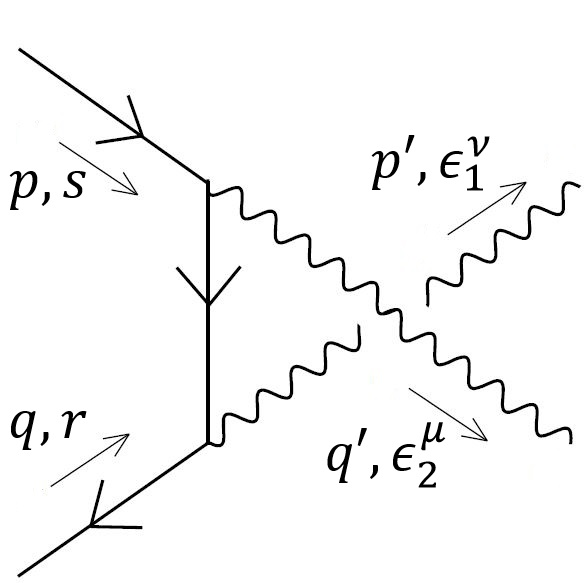
\includegraphics[width=2.2 cm]{pic/eeg2.jpg}\end{aligned}\nonumber\\
=&i(-ie)^2\bar{v}^r(q)\left[\frac{p\!\!\!/-p'\!\!\!\!\!/+m}{(p-p')^2-m^2}+\frac{p\!\!\!/-q'\!\!\!\!\!/+m}{(p-q')^2-m^2}\right]u^s(p)\gamma_\nu\epsilon^\nu_1(p')\gamma_\mu\epsilon_2^\mu(q').
\end{align}
���ڿ��ն�ɢ��, ������
\begin{align}
&i\mathcal{M}^{(2)}=\begin{aligned}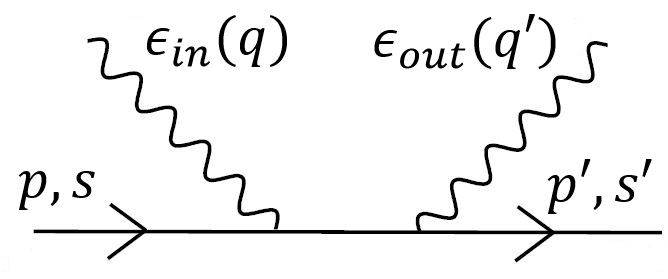
\includegraphics[width=2.8 cm]{pic/comp.jpg}\end{aligned}+\begin{aligned}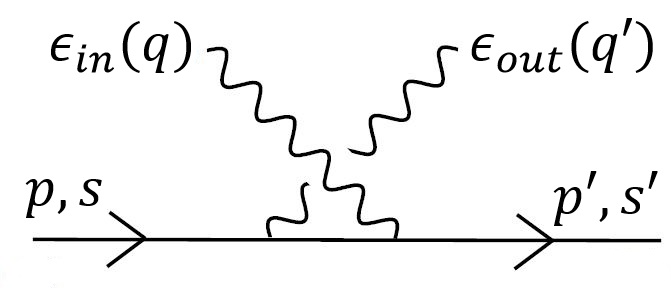
\includegraphics[width=2.8 cm]{pic/comp2.jpg}\end{aligned}\nonumber\\
=&i(-ie)^2\bar{u}^{s'}(p')\left[\frac{\slashed p+\slashed q+m}{(p+q)^2-m^2}+\frac{p\!\!\!/-q'\!\!\!\!\!/+m}{(p-q')^2-m^2}\right]u^s(p)\gamma_\nu\epsilon^\nu_{in}(q)\gamma_\mu\epsilon_{out}^\mu(q').
\end{align}

����, ������  Ϊ��, ���������һ����Ӧ��ɢ�����.












\newpage
\section{Ȧͼ��ɢ��~(��Ȧ) ������: �����ӵ綯��ѧΪ��}

~~~~���ڵ��ɢ������ (���Ժ�Ĵž�����), ��ͼ���Ƽ��ܸ����ȽϺõĽ����. �������, ��һ�����Ǹ߽׼�Ȧͼ����~(��Ϊ��������), ���������õĽ��. Ȼ��д����������ʽ���ѷ���, Ȧͼ�Ƿ�ɢ��. ����������, ����Ҫ������������һ����. �������Ǿ���һ����̽��֮.

ǰһ����, �����Ѽ�ʶ��~$\phi^4$ ���۵�����; ���ߵ���������, �����������ɴ����ӻ�����ͼ~(�����ߴ�����) ��~(�����Ӳ���Լ) ����. �ɱ˴��������, ���Dz��ѵ�֪���ӵĶ�������Ϊ
\begin{align}
-i\Sigma^{(2)}(p)=\begin{aligned}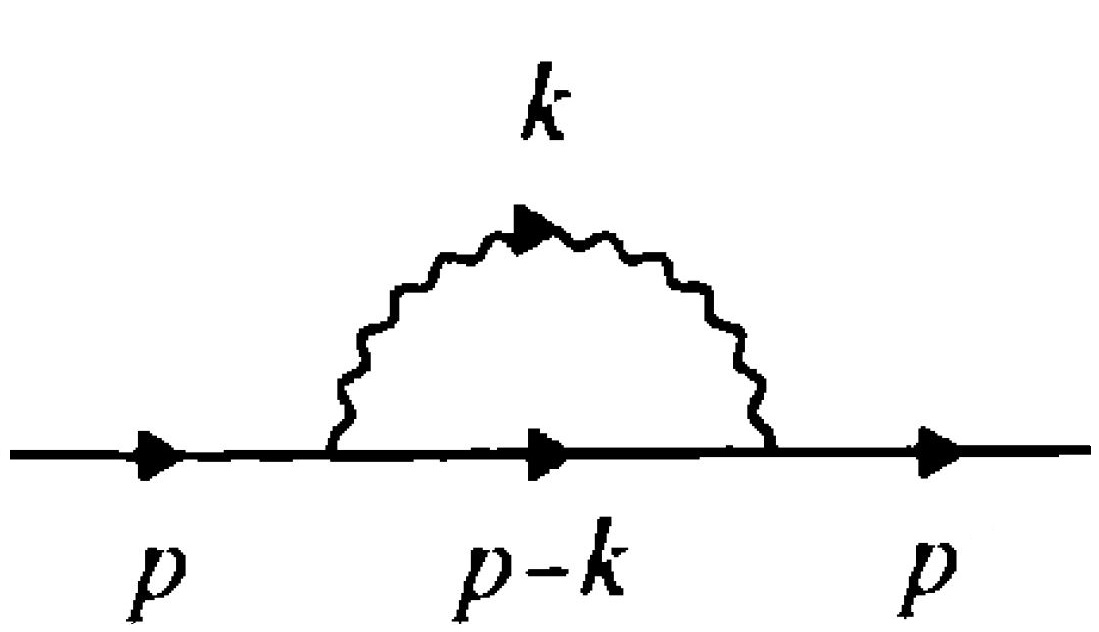
\includegraphics[width=2.5 cm]{pic/eself.jpg}\end{aligned}=(-ie)^2\int\frac{d^4k}{(2\pi)^4}\frac{-ig_{\mu\nu}}{k^2+i\epsilon}\gamma^\mu\frac{i}{\slashed p-\slashed k-m+i\epsilon}\gamma^\nu.
%\not p\not k\slashed{p}\hatslashed{D}\centernot{p} k\!\!\!/
\end{align}
����, ���ӵĶ�������~(�ֿɽж�����ռ���) Ϊ
\begin{align}
i\Pi^{(2)}_{\mu\nu}(k)=\begin{aligned}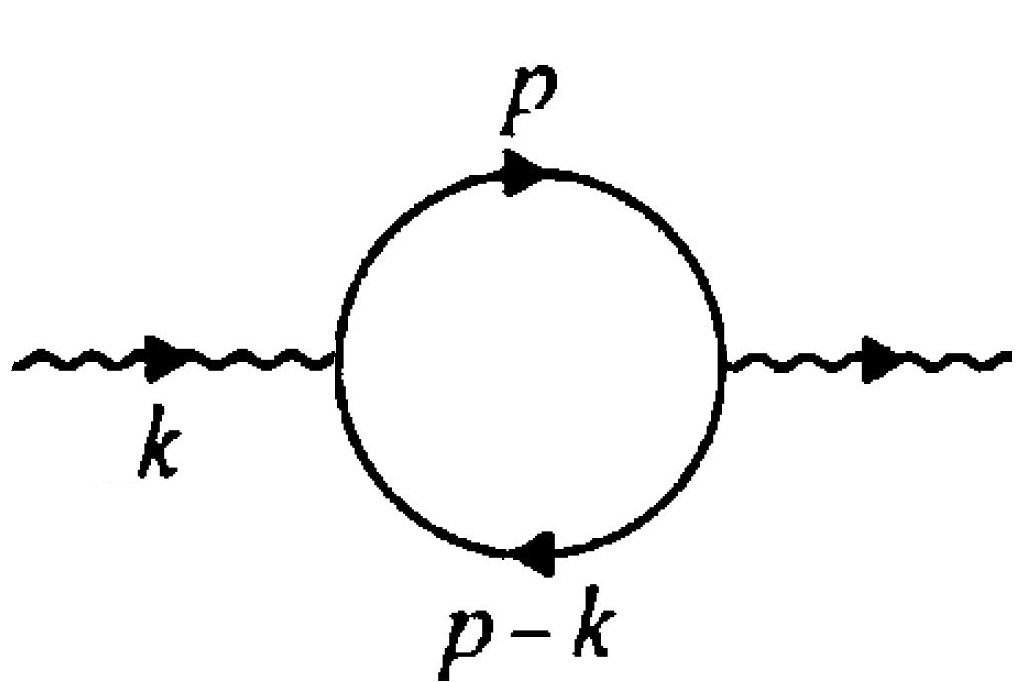
\includegraphics[width=2.7 cm]{pic/pself.jpg}\end{aligned}=(-ie)^2(-1)\int\frac{d^4p}{(2\pi)^4}\operatorname{tr}\left[\gamma_\mu\frac{i}{\slashed p-m}\gamma_\nu\frac{i}{\slashed p-\slashed k-m}\right];
\end{align}
�����Ӳ���Լ����/���涥��/��ȫ����/���Ǻ���~(����ڵ��ӻ���ӵ�����)~$\Gamma_{\mu}$ �Ķ�������~(��������Ŷ���) дΪ
\begin{align}
\Lambda^{(2)}(p)=\begin{aligned}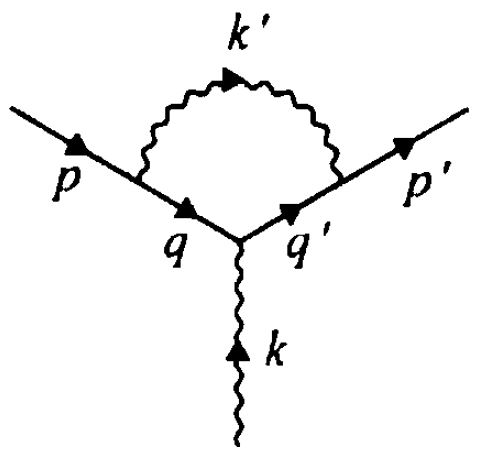
\includegraphics[width=2.5 cm]{pic/vertex2.jpg}\end{aligned}=-ie^2\int\frac{d^4k'}{(4\pi)^4}\frac{1}{k'^2}\gamma_\nu\frac{1}{\slashed{p}'-\slashed{k}'-m}\gamma_\mu\frac{1}{\slashed{p}-\slashed{k}'-m}\gamma^\nu.
\end{align}
��Ȼ, �����������, ���Ƿ�ɢ��. һ���, ���ӳ����еĸ߽�����, ��Ȧͼ, ��������һ����. ������, ��ϵͳ��������Щ��ɢ��һ������.

�������ĵ�һ��, �ǰ�Ȧͼ����еķ�ɢ�������, ��һ���̳�Ϊ���滯. ���滯�ķ���, �нض����滯, ������滯�Լ�ά�����滯~(�������ƹ㵽~$d$ ά, Ȼ������~$d\rightarrow4$) ��. ����, ���Dz��ú���. �ھ���������滯����֮ǰ, ������Ҫ׼��һЩ���ڵ��ά������, ������������ʽ�Լ�~$\Gamma$ �����ȷ����֪ʶ. �����������������ЩԤ������.

����, ���ٷ�����֪, �ƹ㵽~$d$ ά�Ժ�, �Ե��������~$[q]=L^{d/2-2}=\Lambda^{2-d/2}$; �������ǿ���~$q=\mu^{2-d/2}e$, ����~$\mu$ ��Ϊ��������. ���, ���������¹�ʽ
\begin{align}
\frac{1}{ab}=\int^1_0\frac{dx}{\left[ax+b(1-x)\right]^2},
\end{align}
��Ϊ������������ʽ. ����, ����~$\gamma$ ����, ��~$d$ άʱ������~$\{\gamma^\mu,\gamma^\nu\}=2g^{\mu\nu}$, ���������Ȳ�׸��. ���, ����������~$d$ ά���Ͽռ�Ķ������ֹ�ʽ
\begin{align}
\int\frac{d^dp}{(2\pi)^d}\frac{1}{(p^2-m^2)^\alpha}=\frac{(-1)^\alpha i}{(4\pi)^{d/2}}\frac{\Gamma(\alpha-d/2)}{\Gamma(\alpha)}\frac{1}{(m^2)^{\alpha-d/2}}.
\end{align}
��������ƽ�Ʋ�����~$\int d^dpF(p)=\int d^dpF(p+q)$, �Լ��ٽ�ǰ�������~$q$ ������, ���ǻ��ɷֱ�õ�������һʽ�����ʽ
\begin{gather}
\int\frac{d^dp}{(2\pi)^d}\frac{1}{(p^2+2pq-m^2)^\alpha}=\frac{(-1)^\alpha i}{(4\pi)^{d/2}}\frac{\Gamma(\alpha-d/2)}{\Gamma(\alpha)}\frac{1}{(q^2+m^2)^{\alpha-d/2}},\\
\int\frac{d^dp}{(2\pi)^d}\frac{p^\mu}{(p^2+2pq-m^2)^\alpha}=\frac{(-1)^{\alpha-1} i}{(4\pi)^{d/2}}\frac{\Gamma(\alpha-d/2)}{\Gamma(\alpha)}\frac{1}{(q^2+m^2)^{\alpha-d/2}},\\
\int\frac{d^dp}{(2\pi)^d}\frac{p^\mu p^\nu}{(p^2-m^2)^\alpha}=\frac{(-1)^{\alpha-1} i}{(4\pi)^{d/2}}\frac{g^{\mu\nu}\Gamma(\alpha-1-d/2)}{2\Gamma(\alpha)}\frac{1}{(m^2)^{\alpha-1-d/2}}.
\end{gather}
����,


����~QED �����������ܶ�Ϊ
\begin{align}
\mathcal{L}=\bar{\psi}(i\gamma^\mu \partial_\mu-m)\psi-q\bar{\psi}\gamma^\mu\psi A_\mu-\frac{1}{4}F_{\mu\nu}F^{\mu\nu}-\frac{\lambda}{2}(\partial_\mu A^\mu)^2
\end{align}













\subsection{Ward-Takahashi ���ʽ, ��ѧ����}

\newpage
\section{����ɫ����ѧ, ��-Mills ����}

~~~~��һ˼���Ϳɷ���, ʹ��������ɺ˵��໥����, ����ǿ��~(��������, ����) ֮����໥����, ��һ�ֲ�ͬ�������������������µ��໥����; ���dz�Ϊǿ�໥����; �����ʼ�����ֻ����໥����֮һ. ������������ʾ������, ǿ�໥���������ֻ����໥��������ǿ��. �Ա��ڵ���໥���õĽṹ����~$\alpha=\frac{e^2}{4\pi\hbar c}\approx137$, ǿ�໥�����¿���~$\frac{g^2}{4\pi\hbar c}\approx1\sim10$. ����, ǿ�໥������һ�ֶ̳���~(���������Գ�), �����þ���ԼΪԭ�Ӻ��к���֮��ľ���. ���, ǿ�໥���ñ�����������, �и���ĶԳ���, ���и�����غ���. ����ɫ����ѧ����, ��ǿ�໥���ù��Ϊ�ɿ��֮�佻�����Ӷ�����. ���¼����о�֮.

\subsection{���: ����ζ�����ֺ�, ɫ�ռ��~SU(3) �淶�任, ���ֽ���, ��-Mills �淶�������ܶ�}
~~~~
�����~6 ζ: u,~d,~s,~c,~t,~b; �����±�~$f=1,\cdots,6$ ���. ÿζ�ַ�~3 ɫ~(�������Ϸ�����, ��˹���~36 ��): R,~G,~B; �����±�~$n=1,2,3$ ���. ÿζ��˵�������̬, ���ų�һ����ά�ڲ��ռ�, ��Ϊɫ�ռ�, ���Ա�ʾΪ
\begin{align}
\psi=\psi_f=(\psi_1,\psi_2,\psi_3)^T.
\end{align}
ע����������Ϊ 1/2 �ķ�����, ��ÿ��ɫ̬~$\psi_n$ ���ǵ���������. ����~(����) ��˵������ܶȾͿ�дΪ
~$\mathcal{L}_q=\bar{\psi}(i\gamma^\mu\partial_\mu-m)\psi$; ����~$m$ ��Ȼ�ͳ��˾���, ��Ϊ��������. ע����������ɫ�޹�, �������������dz������ĵ�λ��. ���ڿ����������������, һ�ǿ�˵�ɫ����, ��һ�ǽ�������.

�ڿ��ɫ����ά���ռ��ڵı���ʸ�����Ȳ����ת������~$U$~(��~$3\times3$ �ĸ�����, ��~18 ������) �γ�~SU(3) Ⱥ, ������ģ~($\det U=1$) ����~($U^\dag U=1$) ��. �ɴ�, $U$
���������������ֻ��~8 ��. �������DZ�ɽ�~$U$ �����ð˸������Ķ��׾���--��Ϊ�Ƕ�������\footnote{SU(3) �иǶ�������ĵ�λ, ��������~SU(2) �������������ĵ�λ. �������Ǿ���д���Ƕ����������ʽ
\begin{gather}
\lambda_1=\left[\begin{array}{ccc}0&1&0\\1&0&0\\0&0&0\end{array}\right],~\lambda_2=\left[\begin{array}{ccc}0&-i&0\\i&0&0\\0&0&0\end{array}\right],
~\lambda_3=\left[\begin{array}{ccc}1&0&0\\0&-1&0\\0&0&0\end{array}\right],\nonumber\\
\lambda_4=\left[\begin{array}{ccc}0&0&1\\0&0&0\\1&0&0\end{array}\right],~\lambda_5=\left[\begin{array}{ccc}0&0&-i\\0&0&0\\i&0&0\end{array}\right],\nonumber\\
~~~~~~~\lambda_6=\left[\begin{array}{ccc}0&0&0\\0&0&1\\0&1&0\end{array}\right],~\lambda_7=\left[\begin{array}{ccc}0&0&0\\0&0&-i\\0&i&0\end{array}\right],~\lambda_8=\frac{1}{\sqrt{3}}\left[\begin{array}{ccc}1&0&0\\0&1&0\\0&0&-2\end{array}\right].
\end{gather}}--$\lambda^a$ ��ʾΪ
\begin{align}
U=e^{i\theta_a\lambda^a/2}:=e^{i\theta_a T^a},~a=1,\cdots,8.
\end{align}
�Ƕ�������������~$\textrm{tr}\lambda^a=0,~\textrm{tr}\lambda^a\lambda^b=2\delta^{ab}$. SU(3) Ⱥ���������
\begin{align}
[T_a,T_b]=if_{abc}T_c;
\end{align}
���нṹ����~$f_{abc}$ ����������ָ�궼�Ƿ��ԳƵ�. ���ſɱȺ��ʽ~$[A,[B,C]]+[B,[C,A]]+[C,[A,B]]=0$, ���Ƴ���Ⱥ�ṹ��������~$f_{ade}f_{bcd}+f_{bde}f_{cad}+f_{cde}f_{abd}=0$. ��Ⱥ�ṹ������Ϊ��ķ�����
\begin{gather}
f_{123}=1,~f_{458}=f_{678}=\frac{\sqrt{3}}{2},\\
f_{147}=-f_{156}=f_{246}=f_{257}=f_{345}=-f_{367}=\frac{1}{2}.
\end{gather}



��˳���ɫ���ǵĹ淶�任Ϊ~$\psi\rightarrow\psi'=U\psi=e^{i\theta_aT^a}\psi$. ���ɿ�˳���ɫ�ռ�����ϸ������淶������. �����������淶~(��һ������Գ�������Ϊ����
�Գ���, ����������֮Ϊ�淶����Գ���; һ������Գ���ֻ�����ϸ��, ���ܱ��淶) ����Գ���. ��������Ȼ��, ��������Ȼ����һ��ƫ΢�ֵ�Э��΢�̵ı任:
$\partial_\mu\rightarrow D_\mu=\partial_\mu+iqA_\mu$; ��Ҫ��~$D_\mu\rightarrow D'_\mu=\partial_\mu+iq A'_\mu$ ʱ,
\begin{align}
A_\mu\rightarrow A'_\mu=UA_\mu U^\dag+\frac{i}{q}(\partial_\mu U)U^\dag=UA_\mu U^\dag-\frac{i}{q}U\partial_\mu U^\dag,
\end{align}
���ǾͿɵ�~$D_\mu\psi\rightarrow D'_\mu\psi'=UD_\mu\psi=UD_\mu U^\dag\psi'$, ��
\begin{align}
D_\mu\rightarrow D'_\mu=UD_\mu U^\dag.
\end{align}
Ҳ����˵, ����, ���Ǿ͵õ���һ������淶�����������: $\mathcal{L}_{q+qg}=\bar{\psi}(i\gamma^\mu D_\mu-m)\psi=\bar{\psi}(i\gamma^\mu \partial_\mu-m)\psi-q\bar{\psi}\gamma^\mu\psi A_\mu$.


SU(3) Ⱥ����Ԫ���ڲ��ռ�ľ���, һ�㻥������, ������Ⱥ��Ϊ�ǰ�����Ⱥ. �����dz���~SU(3) ��ת�������Զ�����ij�, Ϊ�ǰ�������, ����-Mills �淶��.

������������~$A_\mu$ ��һ������. ��ǰ��~$A_\mu$ �Ĺ淶�任ȡ����, ����~$A^\dag_\mu\rightarrow A'^\dag_\mu=UA^\dag_\mu U^\dag-\frac{i}{q}U\partial_\mu U^\dag$; ���ǿɵ�~$A'^\dag_\mu-A'_\mu=U(A^\dag_\mu-A_\mu)U^\dag$. Ҳ����˵, $A^\dag_\mu-A_\mu=0$ �淶����. �����ζ��, ��������ij�淶��ȡ����~$A_\mu$ �Ƕ��׵�, �������κι淶�¶��Ƕ��׵�.


��Ϊ~$\textrm{tr}T^a=0$, ���Կɵ�~$\textrm{tr}A'_\mu=\textrm{tr}A_\mu$, ���淶���ļ��ǹ淶�����. �������ǿ�ȡ��~$\textrm{tr}A_\mu=0$, ���൱��ȡ��
\begin{align}
A_\mu=A^a_\mu T_a
\end{align}
������ͨ��ɫ��ϵ�~8 ��~��-Mills �淶��~$A^a_\mu$, ��~8 ������. �������ɫ�������໥���õ�����, ����Ϊ~QCD: ����ɫ����ѧ.



������С�淶�任��, $U=e^{i\theta_a T^a}=1+i\theta_a T^a$, ����������~$A_\mu\rightarrow A'_\mu=A_\mu+i\theta^a[T^a,A_\mu]-\frac{1}{q}\partial_\mu\theta_a\cdot T^a$; ��һ���ɵ�~
\begin{align}
A^a_\mu\rightarrow A'^a_\mu=A^a_\mu-f_{abc}\theta^bA^c_\mu-\frac{1}{q}\partial_\mu\theta^a:=A^a_\mu-\frac{1}{q}D_\mu^{ab}\theta^b,
\end{align}
����~$D_\mu^{ab}=\delta^{ab}\partial_\mu+qf_{abc}A^c_\mu$.



���������ҳ���-Mills �淶���������ܶ�. �����˹Τ�����, ��~U(1) �淶������, ���ǾͿɷ���~$[D_\mu,D_\nu]=iqF_{\mu\nu}$; ��~��-Mills ����, ���Ǽ��Ѵ˼���Ϊ�淶��~$F_{\mu\nu}$ �Ķ���:
\begin{align}
F_{\mu\nu}=\frac{1}{iq}[D_\nu,D_\nu]=\partial_\mu A_\nu-\partial_\nu A_\mu+iq[A_\mu,A_\nu].
\end{align}
������ȡ~$\textrm{tr}A_\mu=0$, ������~$\textrm{tr}F_{\mu\nu}=0$, ����������ɽ�~$F_{\mu\nu}$ ��Ϊ~$F_{\mu\nu}=F^a_{\mu\nu}T_a$. ���ǶԴ˷���������ǾͿɵ�~$F^a_{\mu\nu}=\partial_\mu A^a_\nu-\partial_\nu A^a_\mu-qf^{abc}A^b_\mu A^c_\nu$.

���ǿ�����������С�淶�任
\begin{align}
F_{\mu\nu}\rightarrow F'_{\mu\nu}=&UF_{\mu\nu}U^\dag=F^a_{\mu\nu}UT_aU^\dag=F^a_{\mu\nu}T_a+i\theta^bF^a_{\mu\nu}[T^b,T^a]\nonumber\\
=&(F^a_{\mu\nu}-f^{abc}\theta^bF^c_{\mu\nu})T^a,
\end{align}
Ҳ����˵~$F^a_{\mu\nu}\rightarrow F'^a_{\mu\nu}=F^a_{\mu\nu}-f^{abc}\theta^bF^c_{\mu\nu}$. �����, $F_{\mu\nu}$, ����~$-\frac{1}{4}F_{\mu\nu}F^{\mu\nu}$, �Dz����й淶�����Ե�; ͬʱ��ɼ����й淶�����Ե����伣, ��
\begin{align}
\mathcal{L}=-\frac{1}{2}\textrm{tr}F_{\mu\nu}F^{\mu\nu}=-\frac{1}{4}F^a_{\mu\nu}F^{\mu\nu}_a.
\end{align}
����ȡ��ʽΪ��-Mills �淶���������ܶ�.





\subsection{��-Mills ����·���������ӻ�, Faddeev-Popov ����}
~~~~
���п��ܵ�~$A_\mu$, ����������~(�����ù淶�任����ϵ) ���ɹ淶�任��ϵ�ŵ�, �ų�һ�����ռ�; �������ӿռ���Ϊ�˿ռ�ij��������. ��ν�淶����, ����~$A_\mu$ ��ȡֵ�޶���ij�������ϵķ���:
\begin{align}
G^a[A_\mu(x)]=0.
\end{align}
���ڲ�ͬ�淶������������������ǵȼ۵�, ���Դ˳���������ж��ֲ�ͬ��ѡ��, �˴����������ȼ۵�.

ѡ���˳������, ����һ��~(������), ͨ���淶�任�͵õ��ڴ˵��ϵ������������һ������. �����ϲ�ͬ��Ĺ淶���߻����ཻ. ��֮, ����������ͨ���淶�任���ɸ�ά�򲢿ռ�, ��ǰ���ᵽ�ij��ռ�.

Ϊ�˼�������˼��, Faddeev ��~Popov ����İ취, �������淶���ijɷ����в������е�ʽ:
\begin{align}
1=\Delta[A_\mu]\int\mathcal{D}U\delta[G[A^U_\mu]].
\end{align}
����, $A^U_\mu$ ����~$A_\mu$ ͨ���淶�任~$U$ �õ���~$A'_\mu$, ����~$U$ �������Ĺ淶�����ϵ�����ij��; ��~$\delta[G[A^U_\mu]]=\prod_{a,x}\delta\left(G^a[A^U_\mu(x)]\right)$ ��~$\delta$ ����. ����~Faddeev-Popov ��ʽ, ��ʵ�ϼ�~$\Delta[A_\mu]$ �Ķ���. ��Ϊ�������ֽ����һ������ʽ, ���������ֳ�~$\Delta[A_\mu]$ Ϊ~Faddeev-Popov ����ʽ. ��������ι淶�任���ѷ���, Faddeev-Popov ����ʽ�ǹ淶�����, ����
\begin{align}
\Delta[A_\mu]=~\Delta[A^U_\mu].
\end{align}

��������д������~Faddeev-Popov ��ʽ�����ɷ���:
\begin{align}
Z[J]=\int\mathcal{D}A\mathcal{D}U\Delta[A_\mu]\delta[G[A^U_\mu]]e^{iS}=\int\mathcal{D}A\Delta[A_\mu]\delta[G[A_\mu]]e^{iS}.
\end{align}
���ǽ��淶����д��
\begin{align}
G^a[A_\mu(x)]=\Omega^a[A_\mu(x)]-\omega^a(x)=0,
\end{align}
��ɵ����ɷ���Ϊ
\begin{align}
Z[J]=\int\mathcal{D}A\Delta[A_\mu]e^{i(S-\Omega^2/2\xi)}.
\end{align}
����~$-\Omega^2/2\xi$ ���ǹ淶�̶���. ������ȡ~$\Omega^a[A_\mu(x)]=\partial^\mu A_\mu^a$, �͵õ����������˹Τ������ȡ��һ��淶.

Ϊ���ܴ����ɷ�������������, ���ǻ��뽫~Faddeev-Popov ����ʽ��д��ָ����ʽ. ����������Ҫ��, Faddeev-Popov ����ʽ���뱻дΪ~����˹�����ķ�������:
\begin{align}
\Delta[A_\mu]=\int\mathcal{D}\bar{\eta}\mathcal{D}\eta e^{-i\bar{\eta}M\eta}.
\end{align}
���൱��������һ����淶����ϵ���һ�ֳ�~(��ȥ�������ɶȵĴ����ǵ�������������); ���˳���Ȼ�����˸���˹������, ȴ����������, ���Dz�ɫ��. �������ַ�����ϵ, ���ֳ�����������, ���dz�֮Ϊ~Faddeev-Popov ����. ��ֻ������Ȧ��, �������Ϊ����. ��֮, ��-Mills �淶�����������ɷ�������
\begin{align}
Z[J]=\int\mathcal{D}A\Delta[A_\mu]e^{i(S-\Omega^2/2\xi-\bar{\eta}M\eta)};
\end{align}
����
\begin{align}
\mathcal{L}_{\textrm{eff}}=\mathcal{L}_A-\frac{1}{2\xi}\Omega^2-\bar{\eta}M\eta,
\end{align}
�����Ĺ淶�̶��������, ��Ϊ~Faddeev-Popov �����ܶ�.




\subsection{BRST �Գ���}
~~~~
��Э��淶��, �����ʳ�����~Faddeev-Popov �����ܶ�Ϊ
\begin{align}
\mathcal{L}=\bar{\psi}(i\gamma^\mu D_\mu-m)\psi-\frac{1}{4}(F^a_{\mu\nu})^2-\frac{1}{2\xi}(\partial^\mu A^a_\mu)^2-\bar{\eta}^a\partial^\mu D^{ab}_\mu\eta^b.
\end{align}
���ǿ��Խ�����ڹ��Ϊ���ɹ淶�任�������һ����, �����任������Ϊ
\begin{align}
\theta^a=-g\epsilon\eta^a;
\end{align}
����~$\epsilon$ �Ǹ���˹����. ���ǹ淶�����˳��Ĺ淶�任~(����С) ����
\begin{align}
\delta A^a_\mu=\epsilon D_\mu^{ab}\eta^b,~\delta\psi=-ig\epsilon \eta^a T^a\psi.
\end{align}
Ϊ�˱����������ܶ��������任�±��ֲ���, ������Ӧ�����±任��Ϊ
\begin{align}
\delta\eta^a=\frac{1}{2}g\epsilon f^{abc}\eta^b\eta^c,~\delta\bar{\eta}^a=-\frac{\epsilon}{\xi}\partial^\mu A^a_\mu.
\end{align}
����ʽ��ǰ��ʽ, �ϳ�Ϊ~BRST �任. ������֤, �����������ܶ�, ��~BRST �任�µ�ȷ�Dz����.

��~BRST �任�µIJ�����, �ֳ�Ϊ~BRST �Գ���. ��С�������ܶȵ�~BRST �Գ���, ��һ�ֱ任����Ϊ~$\epsilon$ ������Գ���; ���а��������ʳ���淶���Ķ��򲻱���. ��֮�ɼ�, BRST �Գ����Ƕ���淶�Գ��Ե�һ����չ.
%\begin{align}
%\mathcal{L}=\overline{\psi}(i\gamma ^\mu D_\mu -m)\psi+\sum _{k=1}^{\dim (G)}\left[ \frac{-1}{4}F_{\mu\nu}^kF^{\mu \nu k}+\frac{1}{2\xi}(\partial _\mu A^{\mu
%k})^2+\sum _{i=1}^{\dim (G)}\overline{c}^k(-\partial _\mu D^{\mu ki})c^i\right] .
%\end{align}

һ���, ���ǿ��԰�����һ������~BRST �任��Ϊ~$\delta \phi=\epsilon Q\phi$; ����~$Q$ �������ڳ��ϵ����, ��Ϊ~BRST ���. �������һ���������
\begin{align}
Q^2=0;
\end{align}
���ǽ����³�Ϊ~BRST �任����������ݵ�.






\newpage
\section{����ͳһ: GWS ����; ��׼ģ��}

%CKM ���, ���ζ��, ����; �������ƺ�����.

\subsection{�����໥���õ������ܶ�: ������Ϊ��; ��ʼ����������; ��ͬλ��, ������; �²���ת��, ����Ͻ�; Gell-Mann-Nishijima ��ʽ; ��ͬλ���Ĵ�������������}
%�����ѵ�, ��~QED ������, ����໥����Ӱ�����д���ɵ�����, ~QCD ��ǿ�໥����Ӱ�����д�ɫ�ɵ�����; �Ժ󽫷���, ��~GWS ������, ���ǰ����Ӽ�����໥���ù��Ϊ������������ͬλ�������м䲣ɫ�ӵ�����.
~~~~����~$\beta$ ˥���ԭ�Ӻ�/��ԭ�����ӵķ�����˥��, ���б�����һ���ܸı����ӵ�ζ�������Ļ����໥���õIJ���. ���dz������໥����Ϊ���໥����. �����������ֻ����໥���������þ�����̵�, ����ʱ���Ƴ�Ϊ�ķ����ӵ�ֱ�ӵĶ����໥����, �м䲣ɫ���кܴ������. ����, �����ñ���Ҫ�д�����м䲣ɫ��. �ڻ���������, ���໥����Ӱ�����з�����~(����, ���), �Լ�ϣ��˹��ɫ��. ����, ���ǽ�������Ϊ��. ����֪��, 6 ��~(��Ϊ~6 ��ζ; ���Ϸ���������~12��) ���ӹ�������, ���е���~$\mu$ ����~$\tau$ �Ӵ���, ��Ӧ����΢�Ӳ�����, ��������С.

1956 ��, ��������������ָ�������ù��������~$P$ ���غ�. �Ժ����ǽ�һ����ʶ��, �������ù�����~(�Լ����κ�ʱ��), ��΢������������. ��Ϊ���ǽ�һ�����������õ�����, ָ���˷���: ��Ϊ���������������������, �������Ϸ��־���ζ��, ���໥���������ܶ������Ӳ�����������. Ҳ����˵, ���Ǽ����ʼ��������������. (��������������������; ������λ��? �⽫����һ�ڵ�ϣ��˹���Ƹ���.)  �������ǿɽ����ӵĵ��������ܶ�дΪ
\begin{align}
\mathcal{L}_{EW}=\sum_{e:=e,\mu,\tau}i(\bar{e}\gamma^\mu\partial_\mu e+\bar{\nu_e}\gamma^\mu\partial_\mu\nu_e);
\end{align}
���������Ѳ�ȡ���������е�ϰ��, ����ij�����ӵij����ñ������ӵķ��ű�ʾ. ���Ǽ���ÿ�����ӵ���������, ����һ����ά�ڲ��ռ�--��Ϊ��ͬλ���ռ�--��ʸ��, ��Ϊ
\begin{align}
L_e:=\left[\begin{array}{c}\nu_e\\e_L\end{array}\right];
\end{align}
��Ϊ��ͬλ������̬. ��Ȼ, ��ͬλ���ռ����~SU(2) Ⱥ�ĶԳ���, ��ת������/�淶�任Ϊ~$e^{i\alpha^iT^i}=e^{i\alpha^i\sigma^i/2}$; ����~$\sigma^i$ �Ƕ�ά���ռ�ת���ij���Ԫ, ����������. �����ζ��, $L$ ����ͬλ��~$T=1/2$, ��~$TL=\frac{1}{2}\sigma L$; ������ͬλ���ĵ�������, ��΢������Ӧ�ĺɵ��ӷ��������~$T^3=1/2$ ��~$-1/2$. ����, ���Ƕ���~$R_e=e_R$~(��ʵ��, ����˫��̬�뵥̬������ʱ, ����Ӧȡ~$R_e=\left[\begin{array}{c}0\\e_R\end{array}\right]$), ���������ͬλ����ֵΪ~0, ����Ϊ��ͬλ����̬. ����, ���ǿɽ����������ܶȽ�һ����Ϊ
\begin{align}
\mathcal{L}_{EW}=i\bar{L}_e\gamma^\mu\partial_\mu L_e+i\bar{R}_e\gamma^\mu\partial_\mu R_e;
\end{align}
������ȥ����ͷ���, ��ʱ����Ҳ�ɽ��ű�~$e$ ��ȥ. ��ע���ʱ~$\bar{L}=L^\dag\left[\begin{array}{cc}\gamma^0&0\\0&\gamma^0\end{array}\right]$; Ҳ����˵, ����ͬλ������̬����������������������ɵĿռ���, Ҫô��~$\gamma^\mu$ ���ɾ���ֱ���ƶ��Ĺ���, Ҫô��������~$\left[\begin{array}{cc}\gamma^\mu&0\\0&\gamma^\mu\end{array}\right]$.

�������Ǽ����������ù淶�任���о�. ���������ᵽ��~SU(2) �Գ���, ��������������~SU(1) �淶�任~$e^{i\beta Y_W/2}$ ���Dz����; ����~$Y_W$ ��Ϊ���������, ���ڶ���̬�뵥̬�ϵı���ֵ��Ϊ~$Y_W L=Y_L L,~Y_W R=Y_R R$; $Y_{L/R}$ �ľ�����ֵ, ���ǽ����Ժ�ȷ��. ���, ��Ȼ�ɼ�ͬλ���ռ��~$T_W$ �Ǽ򲢵�, ����~$[T^i,Y_W]=0$; �������ǿɵõ����໥���õ����ֹ淶�任�ɺ�дΪ
\begin{align}
U=e^{i\beta Y_W/2+i\alpha^iT^i}.
\end{align}

%����Ƕ�Ӧ����һ�ĺ�, ���ǵ�һ�ĵ���໥�����е����; �ڵ�����, ��һ��Ӧ������, �϶���Ӧ��ͬλ��. ����!

����, �������淶�����໥���õ����ֹ淶�Գ���, �༴��������淶���Ĺ���. ��Ȼ, ���Դ�д��Э��΢�̿�ʼ:
\begin{align}
D_\mu=\partial_\mu+igT^iW_\mu^i+i\frac{1}{2}g'Y_WB_\mu.
\end{align}
�����, Э��΢����������ͬλ����̬�����̬�Ϸֱ�Ϊ
\begin{align}
D_\mu R_e=&\left(\partial_\mu+i\frac{1}{2}g'Y_R B_\mu\right)R_e,\\
D_\mu L_e=&\left(\partial_\mu+ig\frac{1}{2}\sigma^iW_\mu^i+i\frac{1}{2}g'Y_L B_\mu\right)L_e\nonumber\\
=&\partial_\mu L_e+\frac{i}{2}\left[\begin{array}{cc}gW_\mu^3+g'Y_LB_\mu&gW_\mu^1-igW_\mu^2\\gW_\mu^1+igW_\mu^2&-gW_\mu^3+g'Y_LB_\mu\end{array}\right]\left[\begin{array}{c}\nu_e\\e_L\end{array}\right]\nonumber\\
:=&\partial_\mu L_e+\frac{i}{2}\left[\begin{array}{cc}gW_\mu^0+g'Y_LB_\mu&\sqrt{2}gW^+_\mu\\\sqrt{2}gW^-_\mu&-gW_\mu^0+g'Y_LB_\mu\end{array}\right]\left[\begin{array}{c}\nu_e\\e_L\end{array}\right].
\label{weinberg}
\end{align}
���Կ���, ��ʽ��
\begin{align}
W^+_\mu:=\frac{1}{\sqrt{2}}(W_\mu^1-iW_\mu^2),~
W^-_\mu:=\frac{1}{\sqrt{2}}(W_\mu^1+iW_\mu^2)
\end{align}
�Ǿ�����ȷ�����������, ��Ϊ�������໥���õ�����~(�����) �м䲣ɫ��. ͬʱ��ɿ���, $W^0_\mu:=W^3_\mu$ ��~$B_\mu$ ��Ϊͬʱ����΢��������������, ���Բ����ܱ�ڹ��Ϊ�����û������ø��ԵĹ淶��. ���������Ӳ������, ����, �ص���~$W^0_\mu$ ��~$B_\mu$ �ĵ���; ���Ǽ���˵���Ϊһ��ת��:
\begin{align}
\left[\begin{array}{c}A_\mu\\Z^0_\mu\end{array}\right]=\left[\begin{array}{cc}\cos\theta_W&\sin\theta_W\\-\sin\theta_W&\cos\theta_W\end{array}\right]
\left[\begin{array}{c}B_\mu\\W^0_\mu\end{array}\right].
\end{align}
��ʽ��Ϊ�²���ת��, ��~$\theta_W$ ��Ϊ����Ͻ�, ���²����. ���������, ����Ҫȷ���´˽�. ���ѿ���, ��ԭʽ~(\ref{weinberg}) ��, ��~$A_\mu$ ������΢����ϵ����Ǿ��������Ͻ�һ��; �������²���ת�������
\begin{align}
B_\mu=&\cos\theta_W\cdot A_\mu-\sin\theta_W \cdot Z^0_\mu,\\
W^0_\mu=&\sin\theta_W\cdot A_\mu+\cos\theta_W \cdot Z^0_\mu,
\end{align}
�Ϳ����������
\begin{align}
gW_\mu^0+g'Y_LB_\mu=(g\sin\theta_W+g'Y_L\cos\theta_W)A_\mu+(g\cos\theta_W-g'Y_L\sin\theta)Z^0_\mu.
\end{align}
��Ȼ, Ϊ�˰�~$A_\mu$ ڹ��Ϊ����໥���õ��м䲣ɫ��~(����~$Z^0_\mu$ �ͳ��������õĵ������м䲣ɫ��, �Dz������), ���DZ���Ҫ��������΢����û����ϵ�, ��Ҫ��~$g\sin\theta_W+g'Y_L\cos\theta_W=0$; ���ǿɵ�
\begin{align}
\sin\theta_W=\frac{-g'Y_L}{\sqrt{g^2+g'^2Y_L^2}},~\cos\theta_W=\frac{g}{\sqrt{g^2+g'^2Y_L^2}}.
\end{align}
�²���ǵľ�����ֵ, ������ʵ��ó�; ���²�ֵԼΪ~$\sin^2\theta_W=0.2223(21)$. ͨ���򵥵ĵ���, �͵õ��������Ĺ淶��, �²���ת��ʵ������, ����!

����, ������������ǰ�������໥�����еĵ�Ų���; ���~(\ref{weinberg}) �о�������½�һ��:
\begin{align}
D_\mu=&\partial_\mu+ig'\frac{1}{2}Y_W\cos\theta_W A_\mu+igT^3\sin\theta_W A_\mu\nonumber\\
=&\partial_\mu+ig'\cos\theta_W(\frac{Y_W}{2}-Y_LT^3)A_\mu.
\end{align}
��������֪�ĵ�����õ�Э��΢�����Ƚ�, ���ǿɵ�~$g'\cos\theta_W:=e$ �ǻ������; ��Բ�����е�һ�������:
\begin{align}
Q=-Y_LT^3+\frac{Y_W}{2}.
\end{align}
��ʽ��ǿ�໥�����е�~Gell-Mann-Nishijima ��ʽ������ͬ����ʽ. Ҫ��������������ڵ�̬�����̬������ȷ�ĵ��������, ��~$QR=Y_R/2=-1,~QL=Q\left[\begin{array}{c}\nu_e\\e_L\end{array}\right]=
\left[\begin{array}{c}(-Y_L\frac{1}{2}+\frac{Y_L}{2})\nu_e\\(Y_L\frac{1}{2}+\frac{Y_L}{2})e_L\end{array}\right]=\left[\begin{array}{c}0\cdot\nu_e\\1\cdot e_L\end{array}\right]$, ���ǾͿɵó�
\begin{align}
Y_L=-1,~Y_R=-2.
\end{align}
�ݴ�, ���ǿɽ�ǰ�����г���~$Y_L,~Y_R$ ��ʽ�ӽ��л���, ����~$Q=T^3+\frac{Y_W}{2}$, ����
\begin{align}
e=g'\cos\theta_W=\frac{gg'}{\sqrt{g^2+g'^2}}=g\sin\theta_W.
\end{align}
����, ���ǿɽ�һ����ʽ~(\ref{weinberg}) дΪ
\begin{align}
D_\mu L_e=&\partial_\mu L_e+\frac{i}{2}\left[\begin{array}{cc}\sqrt{g^2+g'^2}Z^0_\mu&\sqrt{2}gW^+_\mu\\\sqrt{2}gW^-_\mu&-2eA_\mu+\frac{g'^2-g^2}{\sqrt{g^2+g'^2}}Z^0_\mu\end{array}\right]\left[\begin{array}{c}\nu_e\\e_L\end{array}\right].
\end{align}
д�����ж���淶����, ��������淶����ϵ����������ܶ�, ���Ǽ򵥲���������:
\begin{align}
\mathcal{L}_{\textrm{free+int}}=i\bar{L}_e\gamma^\mu D_\mu L_e+i\bar{R}_e\gamma^\mu D_\mu R_e=\mathcal{L}_{\textrm{free}}+\mathcal{L}_{\textrm{int}};
\end{align}
�����໥���ò���Ϊ
\begin{align}
\mathcal{L}_{\textrm{int}}=&-\frac{1}{2}(\nu_e^\dag,e_L^\dag)\left[\begin{array}{cc}\gamma^0&0\\0&\gamma^0\end{array}\right]
\left[\begin{array}{cc}\sqrt{g^2+g'^2}Z\!\!\!\!/~^0 &\sqrt{2}gW\!\!\!\!\!/~^+\\\sqrt{2}gW\!\!\!\!\!/~^-&-2eA\!\!\!/+\frac{g'^2-g^2}{\sqrt{g^2+g'^2}}Z\!\!\!\!/~^0\end{array}\right]
\left[\begin{array}{c}\nu_e\\e_L\end{array}\right]\nonumber\\
&+\bar{R}_e\left(eA\!\!\!/-\frac{g'^2Z\!\!\!\!/~^0}{\sqrt{g^2+g'^2}}\right)R_e=\mathcal{L}_{eA}+\mathcal{L}_{lW}+\mathcal{L}_{lZ};
\end{align}
���ı����ζ�����໥���������ܶȿɷ�Ϊ��������, ����-$W$ ������Լ�����-$Z$ �����; �������Ƿֱ�д��. ��������Ϊ
\begin{align}
\mathcal{L}_{eA}=e\bar{e}_L\gamma^\mu A_\mu e_L+e\bar{e}_R\gamma^\mu A_\mu e_R=e\sum_{l=e,\mu,\tau}\bar{\psi}_l\gamma^\mu A_\mu \psi_l,
\end{align}
����ȫ����������~QED �еĽ���. ������~$W^\pm$ ��ϵ���Ϊ
\begin{align}
\mathcal{L}_{lW}=-\frac{g}{\sqrt{2}}\sum(\bar{\nu}_e\gamma^\mu W_\mu^+ e_L+\bar{e}_L\gamma^\mu W_\mu^-\nu_e).
\end{align}
���������ҳ��������غ���, ˳������ǰ��~QED ������������, �����������ܶ�������Ϊ����淶����˵���ʽ. Ӧ��ŵ�ض������غ�������ʽ~(\ref{noether cu.}), ���ǿ���������ӳ����غ�ʸ����Ϊ
\begin{align}
j^{\mu i}=\sum \bar{L}_e\gamma^\mu\sigma^iL_e.
\end{align}
������~$j^{\mu\pm}=j^{\mu1}\pm ij^{\mu2},~\sigma^{\pm}=(\sigma^1\pm i\sigma^2)/2$, �����ǿɵ�
\begin{align}
j^{\mu\pm}=\sum 2\bar{L}_e\gamma^\mu\sigma^\pm L_e.
\end{align}
�ɴ�~$\mathcal{L}_{lW}$ �Ϳɽ�һ����Ϊ
\begin{align}
\mathcal{L}_{lW}=-\frac{g}{2\sqrt{2}}\sum(j^{\mu+}W_\mu^++j^{\mu-}W_\mu^-).
\end{align}
���������о�������, �����������Ȳ¶�����������������ʽ��������. ��������д��~$\mathcal{L}_{lZ^0}$ ��:
\begin{align}
\mathcal{L}=&-\frac{1}{2}\left( \sqrt{g^2+g'^2}\bar{\nu}_e\gamma^\mu\nu_eZ_\mu^0+ \frac{g'^2-g^2}{\sqrt{g^2+g'^2}}\bar{e}_L\gamma^\mu e_L Z_\mu^0
+ \frac{2g'^2}{\sqrt{g^2+g'^2}}\bar{e}_R\gamma^\mu e_RZ_\mu^0\right)\nonumber\\
=&-\frac{1}{2}\left( \sqrt{g^2+g'^2}\bar{L}_e\gamma^\mu\sigma^3L_eZ^0_\mu+\frac{2g'^2}{\sqrt{g^2+g'^2}}\bar{e}\gamma^\mu eZ^0_\mu\right)\nonumber\\
=&-\frac{1}{2}\frac{g}{\cos\theta_W}\sum\left(\bar{L}_e\gamma^\mu\sigma^3L_e+2\sin^2\theta_W\bar{e}\gamma^\mu e\right)Z^0_\mu;
\end{align}
%����, ���Ƕ�˭��������ͬ��ֵ. ����, һ��������ѧ�����, ��������Ϊ����, �ֿ��Լ�ָ�����������ڲ�ͬ����̬�ϵ�ֵ�Ƕ���. �����ַ�����һ�µ�.
%������������, �����ı���, һ������. �����ֱ���������ɫ�����.
ǰ��������Ԥ��~$Z^0_\mu$ �Ǵ��������õIJ�����IJ�ɫ��, ������ʽ���Ե�֤: ��������~$Z^0_\mu$ ������������������������΢�����, ����΢�Ӳ�����, �������ܵ������, ����~$Z^0_\mu$ ֻ���Ǵ��������õ��м䲣ɫ��. ����, �����������
\begin{align}
j^{\mu0}:=\bar{L}_e\gamma^\mu\sigma^3L_e+2\sin^2\theta_W\bar{e}\gamma^\mu e
\end{align}
��Ϊ���ӳ���~$Z^0_\mu$ ���Բ�ɫ����ϵ���������. ��������������������Ԥ��, ������ʵ��֤ʵ��. ��һ����, �����ʹ�����ǶԱ�����ͳһ���۵Ľ���.


ǰ���Ѿ��ᵽ��, ���ڵ�����, ���Ǽ����˲���������õij�ʼ������淶���Ӷ�����������. ��ͬ�ڴ˼���, ��ʵ��, �������ӵ�����, ���������õ��м䲣ɫ�Ӷ�����������; ���Һ��ߵ�������ʮ�ֵش�~(����淶�任���ǻ������ǰ�������ò�ɫ��, ���Ǻ��ߵĵ���, ������ʵ���м䲣ɫ����������淶���ӱ����޾�����������Ƶ�ì��, �͵��Խ⿪). ��������ǻ������, ���Ǽ�������һ����̽��.



\subsection{����淶�Գ��Ե��Է���ȱ, ϣ��˹��, Goldstone ����; ������ȱ, ϣ��˹����: �淶���Ե�~Goldstone ��ɫ�ӻ������; $W^\pm,~Z^0$ �Լ����ӵ������Ļ��}

~~~~
��������~$\phi=\chi_1+i\chi_2$ ��~$\phi^4$ ģ��Ϊ
\begin{align}
\mathcal{L}=\partial_\mu\phi^\dag\partial^\mu\phi-m^2\phi^\dag\phi-\lambda(\phi^\dag\phi)^2:=\partial_\mu\phi^\dag\partial^\mu\phi-V(\phi,\phi^\dag);
\end{align}
��ʽ��Ȼ�Ǿ�������淶~$\phi\rightarrow\phi'=e^{i\gamma}\phi$ �����Ե�. ���Ļ�̬/��ն�Ӧ�����ܵļ�С:
\begin{align}
\frac{\partial}{\partial\phi^\dag}V=m^2\phi+2\lambda\phi(\phi^\dag\phi)=0.
\end{align}
��~$m^2>0$, ��ʽ�����ļ�С��Ϊ~$\phi=\phi^\dag=0$, ������ڸ�ƽ���������, ��Ωһ��. ����~$m^2<0$, ��ƽ��������㷴���������ܼ���, �����dz������; ������մ�����
\begin{align}\label{va}
|\phi|^2=\chi_1^2+\chi_2^2=-\frac{m^2}{2\lambda}:=a^2,
\end{align}
��~$|\phi|=a$. Ҳ����˵, �ิƽ��������Ϊ~$a$ ��Բ���ϵ����е�, ���dz������; ������մ���״���������޼򲢵�.

�������Ը�����ն��ǶԳƵ�; �����������, ֻ���������е�һ��, ���پ��й淶�任~(��λ�任, ����ƽ���ڵ�ת��). ���ǰ��������, ��Ϊ��~$\phi$ ��~(��յ�) �Է��Գ���ȱ.


����, ʽ~(\ref{va}) �����, ��������ڴ�ֵΪ~$|\langle0|\phi|0\rangle|^2=a^2$. ��������ڴ��ڲ�Ϊ��ij�, ���dz�֮Ϊϣ��˹��.

\begin{figure}[!h]
\begin{center}
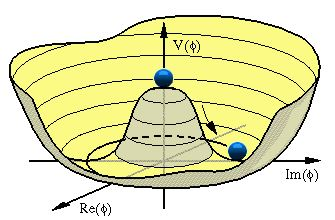
\includegraphics[width=5.0 cm]{pic/mexican.jpg}
\caption{``ī����ñ'' ��: ��������~$\phi^4$ ģ�͵��Է��Գ���ȱ.}
\label{Casimir}
\end{center}
\end{figure}

ʵ���ϲ⵽�ĸ�������, ���dz�����ջ����ϵļ���; ���������������Ļ�̬~$\phi=a$ �������, ����
\begin{align}
\phi=a+\frac{1}{\sqrt{2}}(h+i\rho).
\end{align}
Ҳ����˵, ��ʱ~$h,~\rho$ ���ǿ��Թ۲⵽�������ij���. ������ʽ�Ӵ���ԭʼ�����ܶ�, �ɵ�
\begin{align}
\mathcal{L}=\frac{1}{2}(\partial_\mu h)^2+\frac{1}{2}(\partial_\mu \rho)^2-\lambda v^2h^2-\lambda vh(h^2+\rho^2)-\frac{\lambda}{4}(h^2+\rho^2)^2;
\end{align}
����~$v:=\sqrt{2}a$. �����Ƶ���, Ӧ����ʽ~(\ref{va}), ����ȥ�˳�����. ����ʽ��Ȼ�ɼ�, ��~$h$ ��������
\begin{align}
m_H=\sqrt{2\lambda}v;
\end{align}
ϣ��˹������������, ��Ϊϣ��˹����. ����, �����Կ���, ��~$\rho$ ������. һ���, һ�������Գ��Ե��Է���ȱ, �ᵼ����������/���ӵĴ���, ���Ϊ~Goldstone ����; ��Ӧ�ij�/���Ӿͳ�Ϊ~Goldstone ��/����. ע��˴�ֻ��~Goldstone ������һ��������, ����֤�����ǽ����Ժ����.

��Ȼ����ģ����~$m^2<0$ Ϊ���õ�������Գ��Ե��Է���ȱ, �����Ա��������ڲ��ռ��ʸ��, ��������ȴ�ض��ǷǸ���. ������~$\phi$ ��ij~$N$ ά�ڲ��ռ����ʸ, �������ܶ�һ���дΪ~$\mathcal{L}=\partial_\mu\phi^\dag\partial_\mu\phi-V(\phi)$; ������~$\phi=\phi_0$ ���м�Сֵ, ��~$\frac{\partial V}{\partial\phi_a}\Big|_{a}=0$. ��ô, ���ǿ��ڴ���ո����ļ���, ����
\begin{align}
V(\phi)=&V(\phi_0)+\frac{1}{2}\frac{\partial^2V}{\partial_\mu\phi_a\partial\phi_b}\Big|_{\phi=\phi_0}\delta\phi_a\delta\phi_b+O(\delta\phi^3)\\
:=&V(\phi_0)+\frac{1}{2}m_{ab}\delta\phi_a\delta\phi_b+O(\delta\phi^3).
\end{align}
ֻҪ����ղ����������κ�һ��ƫ��, �����ܱ仯������ֵ, ��������ʽ�ɼ�����~$m_{ab}\geq0$. ����, �����������о��ڲ��ռ�ʸ������~Goldstone ����. ����~$\phi$ ��ij~$N$ ά�ڲ��ռ����ʸ, �������й淶�任~$\phi'=e^{i\theta_a T^a}\phi$. ����, ��������մ��Դ˹淶�任����չ��~(������֮ǰ�ij�����յ�����ƫ��), ����
\begin{align}
V(\phi_0)=V(\phi'_0)=V(\phi_0)+\frac{1}{2}m_{ab}\delta\phi_a\delta\phi_b+\cdots;
\end{align}
���ǿɵ�~$m_{ab}\delta\phi_a\delta\phi_b=0$. ����ζ��, ��~$\delta\phi_a,~\delta\phi_b$ �Բ�Ϊ��, �����~$m_{ab}=0$. ��~$\delta\phi_a$ ��Ϊ��, �⼴������ͬ��̬��Ϊ���, ��˵����շ�����, �Գ����Է���ȱ. �Ӷ�����ȷ֤, �Գ����Է���ȱ, �ص������������ӵĴ���. �˼�~Goldstone ����. ����, �����������̻�����, ��������Ϊ���ά��, ������շ����Է��Գ���ȱ��ά��, ͬʱҲ����~Goldstone ���ӵ���Ŀ~$N_G$; ��������������, ��ϣ��˹�ӵ���Ŀ,  һ��ؼ�~$N-N_G$.

ǰ���������۵�, ������淶�Գ��Ե��Է���ȱ, �����������۶���淶�Գ��Ե��Է���ȱ; �����ֻ��Ϊ�Է��淶��ȱ. �ȿ��ǰ������淶�����; �������Ը�������Ϊ��. ����淶����~$\phi^4$ �����ú�ľ��ж���淶�Գ��Ե������ܶ�Ϊ
\begin{align}
&\mathcal{L}=D_\mu\phi^\dag D^\mu\phi-m^2\phi^\dag\phi-\lambda(\phi^\dag\phi)^2-\frac{1}{4}F_{\mu\nu}F^{\mu\nu}\nonumber\\
=&\partial_\mu\phi^\dag\partial^\mu\phi-m^2\phi^\dag\phi-\lambda(\phi^\dag\phi)^2-iq\phi^\dag\overset{\leftrightarrow}{\partial}_\mu\phi A^\mu+q^2A^2\phi^\dag\phi-\frac{1}{4}F_{\mu\nu}F^{\mu\nu};
\end{align}
��ѡ��~$\phi=a+\frac{1}{\sqrt{2}}(h+i\rho)$, �������ʽ�Ϳɵ�
\begin{align}
\mathcal{L}=&\frac{1}{2}(\partial_\mu h)^2+\frac{1}{2}(\partial_\mu \rho)^2-\lambda v^2h^2-\frac{1}{4}F_{\mu\nu}F^{\mu\nu}+\frac{1}{2}q^2v^2A^2\nonumber\\
&-\lambda vh(h^2+\rho^2)-\frac{\lambda}{4}(h^2+\rho^2)^2+qv\partial_\mu\rho A\nonumber\\
&+qh\overset{\leftrightarrow}{\partial}_\mu\rho A^\mu+q^2vhA^2+\frac{1}{2}q^2(h^2+\rho^2)A^2.
\end{align}
����ʽ�ɶ���, $h,~\rho$ �����������淶������һ����; ������Ϣ��, �淶�����������~$qv$. ����ʽ�ӵڶ������һ��, ����~Goldstone ��ɫ������������. ��ʵ��, ͬ��Ϊ�������Թ����˶�������, Goldstone ��ɫ������ʱ�Dz��ɷֱ��; ����˵�����˵, Goldstone ��ɫ�ӽ��ᱻ���ӳԵ�. ��ѧ��, ����ֱ��������Ϊ��ķ�ʽ������ȥ, ��:
\begin{align}
\mathcal{L}=&\frac{1}{2}(\partial_\mu h)^2-\lambda v^2h^2-\frac{1}{4}F_{\mu\nu}F^{\mu\nu}+\frac{1}{2}q^2v^2A^2\nonumber\\
&-\lambda vh^3-\frac{\lambda}{4}h^4+q^2vhA^2+\frac{1}{2}q^2h^2A^2.
\end{align}
�ɴ�, ���dz����Է��淶��ȱ�����, �淶����ͨ���Ե�~Goldstone ��ɫ��/��ϣ��˹��ɫ�����, �����������. ��������ʹ�淶���ӻ�������Ļ���, �а���ɭ-ϣ��˹����. ��ʵ��, ʹ~Goldstone ��ɫ����ȥ, �൱��ѡȡ���ض��Ĺ淶; ���dz�������ѡ�����, �������淶�������淶. ����һ����ȥ~Goldstone ��ɫ����淶�������~$qv\partial_\mu\rho A$ ������, ��Ϊ~$R_\xi$ �淶, ���Ϊ~'t Hooft �淶, ��������~$\xi$ �淶, ������Ϊ
\begin{align}
\Omega[A_\mu]=\partial_\mu A^\mu-\xi qv\rho;
\end{align}
��˿ɵ�
\begin{align}
-\frac{1}{2\xi}(\partial_\mu A^\mu-\xi qv\rho)^2+qv\partial_\mu\rho A=-\frac{1}{2\xi}(\partial_\mu A^\mu)^2+\frac{1}{2}\xi q^2 v^2\rho^2+qv\partial_\mu(\rho A).
\end{align}
��ʽ���һ����ȫɢ����, ����ֱ����ȥ. �˹淶��, Goldstone ��ɫ����淶�����������ȥ��, ��ǰ������; ������Ϊ������~$\sqrt{\xi}qv$ �Ƿ�������, ������������ȥ. ~$R_\xi$ �淶�ij������ڸ���ʱ�ļ����Լ�����������֤��.



�������ǶԷ������˵һ˵��, �Լ��Ժ������. ��ǰ���Է��淶��ȱΪ��, ����һ�²���ȷ֤, ��ȥ~Goldstone ��ɫ�ӵ������淶, �൱����һ��ʼ��ѡ��
\begin{align}
\phi=\frac{1}{\sqrt{2}}(v+h).
\end{align}
�������������ֱ�ӳ���ʽΪ����/�����淶.

����, �������о���-Mills �淶��������. ���ǿ��Ǿ��и���ά�ڲ��ռ�~(��ͬλ���ռ�) �ĸ�������~$\phi=(\phi^+,\phi^0)^T$. ��~$m^2<0$ ʱ, �˳����������
\begin{align}\label{va}
|\phi|^2=\chi_1^2+\chi_2^2+\chi_3^2+\chi_4^2=-\frac{m^2}{2\lambda}=a^2;
\end{align}
��ʽ���ɲ�����~3 ��, ��ζ�ű������Է��Գ���ȱ������~Goldstone ��ɫ����~3 ��. ��ǰ������, ѡ��
\begin{align}
\phi=\frac{1}{\sqrt{2}}\left[\begin{array}{c}0\\v+H\end{array}\right]
\end{align}
�Ϳ���������~Goldstone ��ɫ�ӱ������õ������淶���Ե�. ���ǿɵ�~$\phi$ ������淶����~$\phi^4$ �����ú�ľ��ж���淶�Գ��Ե������ܶȼ������Ϊ
\begin{align}
&\mathcal{L}=D_\mu\phi^\dag D^\mu\phi-m^2\phi^\dag\phi-\lambda(\phi^\dag\phi)^2-\frac{1}{4}F^i_{\mu\nu}F_i^{\mu\nu}\nonumber\\
=&\partial_\mu\phi^\dag\partial^\mu\phi-i\phi^\dag\overset{\leftrightarrow}{\partial}_\mu\phi A^\mu+q^2A^2\phi^\dag\phi-m^2\phi^\dag\phi-\lambda(\phi^\dag\phi)^2-\frac{1}{4}F^i_{\mu\nu}F_i^{\mu\nu}\nonumber\\
=&\frac{1}{2}(\partial_\mu h)^2+\frac{1}{2}g^2(v+h)^2A^2-\frac{\lambda}{4}(h^4+4vh^3+4v^2h^2-v^4)-\frac{1}{4}F^i_{\mu\nu}F_i^{\mu\nu}\nonumber\\
=&-\frac{1}{4}F^i_{\mu\nu}F_i^{\mu\nu}+\frac{1}{2}g^2v^2A^2+\frac{1}{2}(\partial_\mu h)^2-\lambda v^2h^2\nonumber\\
&-\lambda vh^3-\frac{1}{4}\lambda h^4+g^2vhA^2+\frac{1}{2}g^2h^2A^2.
\end{align}
����~$D_\mu=\partial_\mu+igT^iW_\mu^i:=\partial_\mu+igA_\mu$. --Ϊ���������, Ŀǰ������δ����~U(1) ����; ���ǽ����Ժ���������. --���������һ���ǹ淶������ϣ��˹��, �ڶ���ǰ������ϣ��˹�ӵ������, ����������淶�������. �������, �淶����Ȼ���������. �������ǿ�������~Goldstone ��ɫ�ӵĴ������. ���Ǽ��賡����������~$Y_W\phi=Y_H\phi$, ��Ӧ��~Gell-Mann-Nishijima ��ϵ, �ɵ�
\begin{align}
Q\phi=\left(T^3+\frac{Y_W}{2}\right)\phi=\left(T^3+\frac{Y_H}{2}\right)\phi=\frac{1}{2}\left[\begin{array}{c}(1+Y_H)\phi^+\\(-1+Y_H)\phi^0\end{array}\right]
\end{align}
��ղ�����, ��������ʽ�ɵ�~$Y_H=1$; ��һ���ɵ�~$\phi^+$ �е��~$+1$. Ҳ����˵, ���������м䲣ɫ�ӳԵ�������~Goldstone ��ɫ��, ������������, һ��������; ��ʣ�µ����һ�����Ӽ�ϣ��˹��ɫ��, �ǵ����Ե�.

����, ����д��~U(1)$\otimes$SU(2) Э�����~$U=e^{i\beta Y_W/2+i\alpha^iT^i}$ �����ڳ�~$\phi=(\phi^+,\phi^0)^T$ �ϵ�������ʽ:
\begin{align}
D_\mu\phi=&\partial_\mu\phi+\frac{i}{2}\left[\begin{array}{cc}gW_\mu^0+g'Y_HB_\mu&\sqrt{2}gW^+_\mu\\\sqrt{2}gW^-_\mu&-gW_\mu^0+g'Y_HB_\mu\end{array}\right]
\left[\begin{array}{c}\phi^+\\\phi^0\end{array}\right]\nonumber\\
=&\partial_\mu\phi+\frac{i}{2}\left[\begin{array}{cc}gW_\mu^0+g'B_\mu&\sqrt{2}gW^+_\mu\\\sqrt{2}gW^-_\mu&-gW_\mu^0+g'B_\mu\end{array}\right]
\left[\begin{array}{c}\phi^+\\\phi^0\end{array}\right]\nonumber\\
=&\partial_\mu\phi+\frac{i}{2}\left[\begin{array}{cc}2eA_\mu-\frac{g'^2-g^2}{\sqrt{g^2+g'^2}}Z^0_\mu&\sqrt{2}gW^+_\mu\\\sqrt{2}gW^-_\mu&-\sqrt{g^2+g'^2}Z^0_\mu\end{array}\right]\left[\begin{array}{c}\phi^+\\\phi^0\end{array}\right]\nonumber\\
:=&\partial_\mu\phi+\frac{i}{2}\mathscr{D}_\mu\phi;
\end{align}
����~$\mathscr{D}_\mu^\dag=\mathscr{D}_\mu$. �������ǿɵ�
\begin{align}
(D_\mu\phi)^\dag D^\mu\phi=\partial_\mu\phi^\dag\partial^\mu\phi+\textrm{Im}(\phi^\dag\mathscr{D}_\mu\partial^\mu\phi)+\frac{1}{4}\phi^\dag\mathscr{D}_\mu\mathscr{D}^\mu\phi.
\end{align}
��ǰ��ѡ�������/Goldstone ��ɫ�ӷ���ʽ, ��ͬλ���ռ�������淶������ʽ, �Ϳɵó����Ļ�������Լ��淶��������ij���; �����һ����~$\partial_\mu\phi^\dag\partial^\mu\phi=\frac{1}{2}(\partial_\mu H)^2$ ��ϣ��˹���Ķ����ܶ�; ���߲���. ����, �淶���������������ʽ���һ��������~$(0,v/\sqrt{2})^T$ ������֮��. ����
\begin{align}
&\frac{1}{4}\left[\begin{array}{c}0\\\frac{v}{\sqrt{2}}\end{array}\right]^\dag\mathscr{D}^\mu\mathscr{D}_\mu\left[\begin{array}{c}0\\\frac{v}{\sqrt{2}}\end{array}\right]\nonumber\\
=&\frac{1}{4}\frac{v}{\sqrt{2}}\left[\begin{array}{c}\sqrt{2}gW^{+^\mu}\\-\sqrt{g^2+g'^2}Z^{0\mu}\end{array}\right]^\dag
\left[\begin{array}{c}\sqrt{2}gW^+_\mu\\-\sqrt{g^2+g'^2}Z^0_\mu\end{array}\right]\frac{v}{\sqrt{2}}\nonumber\\
=&\frac{1}{4}g^2v^2W^{-\mu}W^+_\mu+\frac{1}{8}(g^2+g'^2)v^2Z^{0\mu}Z^0_\mu.
\end{align}
�������Ǿ͵�
\begin{align}
m_W=\frac{1}{2}gv,~m_Z=\frac{1}{2}\sqrt{g^2+g'^2}v=\frac{m_W}{\cos\theta_W}.
\end{align}
������������, ����ʵ��ó�. ֵ��ע�����, �ԼӼ��㲻�ѷ���, ����������һ��������, ����û�ܲ���������, ��Ȼ���־�����Ϊ��. ����ؿ���˵, ����~Goldstone ��ɫ�ӷֱ�������õ������淶���ӳԵ���; ����û����, ����û�ܻ������. ��֮, �û�������Ļ����, ���û��������û���: ���ǵ����۵�ȷ��ǡ����ݵ�.% ͨ������, ��������;
~��˽��, ��������!



%\begin{align}
%\mathscr{D}_\mu\left[\begin{array}{c}0\\\frac{v}{\sqrt{2}}\end{array}\right]=&\left[\begin{array}{cc}2eA_\mu-\frac{g'^2-g^2}{\sqrt{g^2+g'^2}}Z^0_\mu&\sqrt{2}gW^+_\mu\\\sqrt{2}gW^-_\mu&-\sqrt{g^2+g'^2}Z^0_\mu\end{array}\right]
%\left[\begin{array}{c}0\\\frac{v}{\sqrt{2}}\end{array}\right]\nonumber\\
%=&\left[\begin{array}{c}\sqrt{2}gW^+_\mu\\-\sqrt{g^2+g'^2}Z^0_\mu\end{array}\right]\frac{v}{\sqrt{2}}
%\end{align}

�������, ������������������. ��;��, ��������ȥ��~Goldstone ��ɫ��, ����ϣ��˹���������. ����������ϣ��˹��֮�����������, ���д��
\begin{align}
\mathcal{L}_{lH}=-\sum_{e,\mu,\tau} g_e(\bar{L}_e\phi R_e+\bar{R}_e\phi^\dag L_e);
\end{align}
��Ȼǰ�����Ϊ���׹���. �������淶������ʽ, �͵�
\begin{align}
\mathcal{L}_{lH}=&-\sum_{e,\mu,\tau} g_e\bar{e}e\phi^0:=-\sum_{e,\mu,\tau}\left(m_e\bar{e}e+\frac{m_e}{v}\bar{e}eH\right);
%=-\frac{1}{\sqrt{2}}\sum g_e\left[\bar{L}_e(v+H)R_e+\bar{R}_e(v+H)L_e\right]\nonumber\\
\end{align}
�ɴ�ʽ��ɼ�, ��΢��δ����������, Ҳδ��ϣ��˹�������. ���������ӻ��������, Ϊ
\begin{align}
m_e=\frac{g_ev}{\sqrt{2}}.
\end{align}





%ע��: R_e ��ʱ���ǰ�ά��, ��ʱ��������ά��, ��������~~~~~~~~~~~~~~~~`��ʵR_e Ӧ�ǰ�ά, e_R ������ά. �����������ȽϺ�. ���е�ʱ���ֲ�������. ��Ϊ�������������, ������һ��������ά.



%��ָ���໥���õ�һЩ�����ص�.
%ѡ�淶, ����ѡ��λ. ѡ�����ĸ��ط�����.
\subsection{��˵�������, CKM ����}

~~~~
����������~$(\nu_e,e),~(\nu_\mu,\mu),~(\nu_\tau,\tau)$ ���Ƶ�, ���Ҳ��Ϊ����~$(u,d),~(c,s),~(t,b)$. ��˹��ɵ���ͬλ��˫��̬�뵥̬����
\begin{gather}
L_u=\left[\begin{array}{c}u_L\\d_L\end{array}\right],~L_c=\left[\begin{array}{c}c_L\\s_L\end{array}\right],~L_t=\left[\begin{array}{c}t_L\\b_L\end{array}\right];\\
R_u=u_R,~R_c=c_R,~R_t=t_R,\\
R_d=d_R,~R_s=s_R,~R_b=b_R.
\end{gather}
����, $u,~c,~t$ ��˾��е��~$2/3$; $d,~s,~b$ ��˾��е��~$-1/3$. ����, ��~Gell-Mann-Nishijima ��ʽ, ���Ǿ�֪
\begin{align}
QL_u=\left(T^3+\frac{Y_W}{2}\right)\left[\begin{array}{c}u_L\\d_L\end{array}\right]=\left[\begin{array}{c}
\left(\frac{1}{2}+\frac{Y_W}{2}\right)u_L\\\left(-\frac{1}{2}+\frac{Y_W}{2}\right)d_L\end{array}\right],
\end{align}
Ҳ����˵�����ͬλ������̬����������~$Y_{uL}=\frac{1}{3}$. ���Ƶ�, $QR_u=\frac{Y_W}{2}R_u=\frac{2}{3},~QR_d=\frac{Y_W}{2}R_d=-\frac{1}{3}$, ��~$u,~c,~t$ ��̬����������~$Y_{uR}=\frac{4}{3}$, ��~$d,~s,~b$ ��̬����������~$Y_{dR}=-\frac{2}{3}$.

ĿǰΪֹ, ���Ǽ�����������������. ����, �����ÿ����ϣ��˹�����, ��ʹ֮�������. �����ϣ��˹����������Ͽ�дΪ
\begin{align}
\mathcal{L}_{qH}=-\sum_{ud,cs,tb}(g_d\bar{L}_u\phi R_d+g_u\bar{L}_u\phi_CR_u+h.c.)
\end{align}
����, $\phi_C=i\sigma^2\left[\begin{array}{c}\phi^+\\\phi^0\end{array}\right]=\left[\begin{array}{c}\phi^0\\-\phi^-\end{array}\right]$ Ϊ~$\phi$ �ĵ�ɹ���̬~(����~Gell-Mann-Nishijima ��ʽ���ѷ���~$\phi_C$ ��������~$-1$). ���׷���, ����������, ֮����û�������ڶ���, ����Ϊ�������������غ�. ����, ����ѡ�������淶, ���ÿ�˳Ե�~Goldstone ��ɫ��. ע��~$\phi$ �������淶����ǰ��; ��~$\phi_C$ �Ĺ淶Ϊ~$\phi_C=\frac{1}{\sqrt{2}}\left[\begin{array}{c}v+H\\0\end{array}\right]$. �������淶��, ������
\begin{align}
\mathcal{L}_{qH}=&-\sum_{ud,cs,tb} (g_d\bar{d}_L\phi^0 d_R+g_u\bar{u}_L\phi^0u_R+h.c.)\nonumber\\
=&-\sum_qg_q\bar{q}q\phi^0:=-\sum_q\left(m_q\bar{q}{q}+\frac{m_q}{v}\bar{q}qH\right);
%=-\sum_q\left(\frac{g_qv}{\sqrt{2}}\bar{q}{q}+\frac{g_qH}{\sqrt{2}}\bar{q}q\right)\nonumber\\
\end{align}
���������һ���ǿ�˵�������, �ڶ����ǿ����ϣ��˹�������. �ɴ˼�, ��˻��������
\begin{align}
m_q=\frac{g_qv}{\sqrt{2}}.
\end{align}


��ͬ�������������õ�, ����~$B_\mu,~W^0_\mu$ ���²���ת�����Ӷ��ɵ�~$A_\mu,~Z^0_\mu$ һ��, �����δ��������������̬, �����������̬�����ݲ��뵽���໥������ȥ��. ����ζ���������ù�����, ��˿��ܻ���ζ��~(�����, �Ժ����ǽ�ȷ֤, ʹ��˷���ζ�伴������ϵ�, ������~$W^\pm_\mu$ ���粣ɫ�ӵ��໥����). �������ǿ���
\begin{align}
\left[\begin{array}{c}u_{1L/R}\\u_{2L/R}\\u_{3L/R}\end{array}\right]=U_{L/R}\left[\begin{array}{c}u_{L/R}\\c_{L/R}\\t_{L/R}\end{array}\right],~
\left[\begin{array}{c}d_{1L/R}\\d_{2L/R}\\d_{3L/R}\end{array}\right]=D_{L/R}\left[\begin{array}{c}d_{L/R}\\s_{L/R}\\b_{L/R}\end{array}\right];
\end{align}
����~$U,~D$ ��~$3\times3$ ���Ͼ���. ���Ƿֱ��~$u_i,~d_i$ ��~$u$ ������~$d$ ����. ���ͬʱ, ���乹�ɵ���ͬλ������̬�뵥̬����
\begin{gather}
L_i=\left[\begin{array}{c}u_{iL}\\d_{iL}\end{array}\right],~R_{ui}=u_{iR},~R_{di}=d_{iR}.
\end{gather}
���ѷ���, �任���̬��֮ǰ�ľ���ͬ���ĵ��, ����������ͬλ��. ����ֱ�ӿ���
\begin{gather}
\mathcal{L}_q=\sum_qi\bar{q}\gamma^\mu\partial_\mu q=\sum_{ud,cs,tb}\left(i\bar{L}_u\gamma^\mu\partial_\mu L_u+i\bar{R}_u\gamma^\mu\partial_\mu R_u+i\bar{R}_d\gamma^\mu\partial_\mu R_d\right).
\end{gather}
%ע���һ��, ���Գ�~6 �������������ʽ.
%����~$R_u$ ��ɿ��������ų�һ����ʸ. ��Ȼ, ����٤�����Ҫô��һ���Ǿ��󻯿������ƶ��ķ���, Ҫô�ǵ������µ���ʽ������ά��λ��.
������������������, �����ֿɽ�һ������ʽ��Ϊ
\begin{gather}
\mathcal{L}_q=\sum_i\left(i\bar{L}_i\gamma^\mu\partial_\mu L_i+i\bar{R}_{ui}\gamma^\mu\partial_\mu R_{ui}+i\bar{R}_{di}\gamma^\mu\partial_\mu R_{di}\right);
\end{gather}
�����õ���~$U,~D$ ���Ͼ�����һ����. ��ִ�г���һ������, ��������ǿ�໥���õľ��ǿ�˵���������̬, ǿ�����п����ζ��. ��ʵ��, ��Ȼ, ֻҪ���ҷ���û�����, ���������������~$\sum_ii\bar{R}_{ui}\gamma^\mu\partial_\mu R_{ui}=\sum_{ud,cs,tb}i\bar{R}_u\gamma^\mu\partial_\mu R_u$ ���Ľ��; Ҳ����˵��˾�������������̬����, ����˾���ζ��. �������о��Ŀ�˵ĵ�����ü������~$Z^0_\mu$ ��ɫ�ӵ�����, �Ͷ����������. ��������ϵĻ�, ��Ȼ���ǽ�����һ������, �˼�~CKM~(Cabibbo�CKobayashi�CMaskawa, ���Ȳ�-С��-�洨) ����; �⽫�ڿ����~$W^\pm_\mu$ ������ʱ����. ����, ���Ǿ����ֱ��о�.


��ƫ΢�ָijɵ������õ�Э��΢��~$D_\mu=\partial_\mu+igT^iW_\mu^i+i\frac{1}{2}g'Y_WB_\mu$, ���Ǿ͵õ��˿�˲�������໥���õ�ģ��:
\begin{align}
\mathcal{L}_{q+qWZ}=&i\bar{L}_i\gamma^\mu D_\mu L_i+i\bar{R}_{ui}\gamma^\mu D_\mu R_{ui}+i\bar{R}_{di}\gamma^\mu D_\mu R_{di}\nonumber\\
=&\mathcal{L}_q+\mathcal{L}_{qA}+\mathcal{L}_{qZ^0}+\mathcal{L}_{qW^\pm}.
\end{align}
��һ��ʽ~(\ref{weinberg}) ��Ͽ�˵�̬�����̬��������, ���ѵõ�
\begin{align}
D_\mu R_{ui}&=\left(\partial_\mu+i\frac{2}{3}g'B_\mu\right)R_{ui}\nonumber\\
&=\left(\partial_\mu+i\frac{2}{3}g'(A_\mu\cos\theta_W-Z^0_\mu\sin\theta_W)\right)R_{ui},\\
D_\mu R_{di}&=\left(\partial_\mu-i\frac{1}{3}g'B_\mu\right)R_{di}\nonumber\\
&=\left(\partial_\mu-i\frac{1}{3}g'(A_\mu\cos\theta_W-Z^0_\mu\sin\theta_W)\right)R_{di},\\
D_\mu L_i&=\partial_\mu L_i+\frac{i}{2}\left[\begin{array}{cc}gW_\mu^0+\frac{1}{3}g'B_\mu&\sqrt{2}gW^+_\mu\\\sqrt{2}gW^-_\mu&-gW_\mu^0+\frac{1}{3}g'B_\mu\end{array}\right]L_i;
\end{align}
��Ϊд������, �������ǰ��������һʽ�о����ڶԽ�����²���ת������������:
\begin{align}
&g\sin\theta_W A_\mu+gZ^0_\mu\cos\theta_W+\frac{1}{3}g'A_\mu\cos\theta_W-\frac{1}{3}g'Z^0_\mu\sin\theta_W,\\
-&g\sin\theta_W A_\mu-gZ^0_\mu\cos\theta_W+\frac{1}{3}g'A_\mu\cos\theta_W-\frac{1}{3}g'Z^0_\mu\sin\theta_W.
\end{align}
����, ���ǾͿ�ֱ���ó����໥��������. ���˵ĵ���໥������Ϊ
\begin{align}
\mathcal{L}_{qA}=&-\frac{1}{2}(\bar{u}_{iL},\bar{d}_{iL})\left[\begin{array}{cc}eA_\mu+\frac{1}{3}eA_\mu&0\\0&-eA_\mu+\frac{1}{3}eA_\mu\end{array}\right]
\left[\begin{array}{c}u_{iL}\\d_{iL}\end{array}\right]\nonumber\\
&-\frac{2}{3}e\bar{u}_{iR}\gamma^\mu u_{iR}A_\mu+\frac{1}{3}e\bar{d}_{iR}\gamma^\mu d_{iR}A_\mu\nonumber\\
=&-\frac{2}{3}e\bar{u}_{iL}\gamma^\mu u_{iL}A_\mu+\frac{1}{3}e\bar{d}_{iL}\gamma^\mu d_{iL}A_\mu-\frac{2}{3}e\bar{u}_{iR}\gamma^\mu u_{iR}A_\mu+\frac{1}{3}e\bar{d}_{iR}\gamma^\mu d_{iR}A_\mu\nonumber\\
=&\sum_i\left(-\frac{2}{3}e\bar{u}_{i}\gamma^\mu u_{i}A_\mu+\frac{1}{3}e\bar{d}_{i}\gamma^\mu d_{i}A_\mu\right)\nonumber\\
=&\sum_{ud,cs,tb}\left(-\frac{2}{3}e\bar{u}\gamma^\mu uA_\mu+\frac{1}{3}e\bar{d}\gamma^\mu dA_\mu\right)=\sum_q e\bar{q}\gamma^\mu Q qA_\mu.
\end{align}
����~$Q$ Ϊ��˵ĵ�����. ������~QED �е�һ����ʽ. ���濼������~$Z^0_\mu$ ��ɫ�ӵ����.%�����ӵ�������ʽ�������ڶ�ʽ, �Կ�˻��̬����ͻ�Ϊ�Կ��ζ�����; ��˫������ʽ�����������໥���õ�, �Կɹ鵽��˵���������̬.
\begin{align}
\mathcal{L}_{qZ^0}=&\left(\frac{2}{3}\bar{u}_{iR}\gamma^\mu u_{iR}-\frac{1}{3}\bar{d}_{iR}\gamma^\mu d_{iR}\right)g'\sin\theta_WZ^0_\mu\nonumber\\
&-\left(\frac{1}{2}g\cos\theta_W-\frac{1}{6}g'\sin\theta_W\right)\bar{u}_{iL}\gamma^\mu u_{iL}Z^0_\mu\nonumber\\
&-\left(-\frac{1}{2}g\cos\theta_W-\frac{1}{6}g'\sin\theta_W\right)\bar{d}_{iL}\gamma^\mu d_{iL}Z^0_\mu\nonumber\\
=&\bar{q}_{R}\gamma^\mu Qq_{R}g'\sin\theta_WZ^0_\mu\nonumber\\
&-\frac{g}{\cos\theta_W}\left(\frac{1}{2}-\frac{2}{3}\sin^2\theta_W\right)\bar{u}_{L}\gamma^\mu u_{L}Z^0_\mu\nonumber\\
&-\frac{g}{\cos\theta_W}\left(-\frac{1}{2}+\frac{1}{3}\sin\theta^2_W\right)\bar{d}_{L}\gamma^\mu d_{L}Z^0_\mu\nonumber\\
=&-\frac{g}{\cos\theta_W} \left[\bar{q}_{L}\gamma^\mu\left(T^3-Q\sin\theta^2_W\right) q_{L}-\bar{q}_{R}\gamma^\mu Q\sin^2\theta_W q_{R} \right] Z^0_\mu\nonumber\\
=&-\frac{g}{\cos\theta_W} \left[\bar{q}_{L}\gamma^\mu T^3q_{L}-\bar{q}\gamma^\mu Q\sin^2\theta_W q \right] Z^0_\mu
\end{align}
����ʽ������-$Z^0_\mu$ �����ʽ�����Ƶ�; ���������ǿ����ͬλ����������. �����~$W^\pm_\mu$ ������Ǻܺ��ó���:
\begin{align}
\mathcal{L}_{qW^\pm}=&-\frac{g}{\sqrt{2}}\left(\bar{u}_{iL}\gamma^\mu d_{iL}W^+_\mu+\bar{d}_{iL}\gamma^\mu u_{iL}W^-_\mu\right)\nonumber\\
=&-\frac{g}{\sqrt{2}}\left(\bar{u}_{L}\gamma^\mu V_{ud}d_{L}W^+_\mu+\bar{d}_{L}\gamma^\mu V^*_{du} u_{L}W^-_\mu\right);
\end{align}
������ά�Ͼ���
\begin{align}
V=U_L^\dag D_L
\end{align}
��Ϊ~CKM ����; ��������˲�ͬζ��Ļ��, ����Ҫ��ʵ�����ⶨ��. �����²�ֵ�ɼ��������; ���Ƶ�, ��ԼΪ
\begin{align}
V=\left[\begin{array}{ccc}
\cos\theta_c&\sin\theta_c&0\\
-\sin\theta_c&\cos\theta_c&0\\
0&0&1
\end{array}
\right];
\end{align}
����~$\theta_c$ ��Ϊ~Cabibbo ��. Ҳ����˵~CKM ����������һ����ά�ռ������ת��.





%CKM ����: �.



\subsection{���������ı�׼ģ��}


~~~~�ܽ�����, ��������ͳһ��~Glashow-Weinberg-Salam ���۵������ܶȾ���
\begin{align}
\mathcal{L}_{\textrm{GWS}}=&\mathcal{L}_{\textrm{gauge field}}+\mathcal{L}_{\textrm{lepton+G~bosons}}+\mathcal{L}_{\textrm{quark+G~Bosons}}\nonumber\\
&+\mathcal{L}_{\textrm{Higgs+$\phi^4$}}+\mathcal{L}_{\textrm{lepton+Higgs}}+\mathcal{L}_{\textrm{quark+Higgs}}\nonumber\\
=&-\frac{1}{4}B_{\mu\nu}B^{\mu\nu}-\frac{1}{4}W^i_{\mu\nu}W_i^{\mu\nu}\nonumber\\
&+\left(i\bar{L}_e\gamma^\mu D_\mu L_e+i\bar{R}_e\gamma^\mu D_\mu R_e\right)\nonumber\\
&+\left(i\bar{L}_i\gamma^\mu\partial_\mu L_i+i\bar{R}_{ui}\gamma^\mu\partial_\mu R_{ui}+i\bar{R}_{di}\gamma^\mu\partial_\mu R_{di}\right)\nonumber\\
&+D_\mu\phi^\dag D^\mu\phi-m^2\phi^\dag\phi-\lambda(\phi^\dag\phi)^2\nonumber\\
&-g_e(\bar{L}_e\phi R_e+\bar{R}_e\phi^\dag L_e)\nonumber\\
&-(g_d\bar{L}_u\phi R_d+g_u\bar{L}_u\phi_CR_u+h.c.);
\end{align}
��~$D_\mu=\partial_\mu+igT^iW_\mu^i+i\frac{1}{2}g'Y_WB_\mu$, ����������, ��Ի~SU(2)$\otimes$U(1) �Գ����µ�Э�䵼��. ���ټ��Ͻ��ӳ���������~$\mathcal{L}_{\textrm{gluon}}=-\frac{1}{4}F^a_{\mu\nu}F_a^{\mu\nu}$, ����~SU(3) �µ�Э�䵼���ӽ���, ��
\begin{align}
D_\mu=\partial_\mu+igT^iW_\mu^i+i\frac{1}{2}g'Y_WB_\mu+ig_3T^aA^\mu_a,
\end{align}
�����Ǿ͵õ���ͬʱ����ǿ, ����������������������������. ������Э�䵼�����������ܶȼ������̺���һϵ��˼��ԭ�������㷽��, ��Ϊ���������ı�׼ģ��.











%������ɵ�ɳе�, ����, ����֪�ɵ����е�; ͬ��, ����, �����������е�
%����ڵ��, ��������, ����ͬλ��.!!!!!!!!��ν����, ����ͬλ����.
%��Ϊ��һ, ���㷴����, ����ֻ��һ��, �������ܸ��ܵ���. ��ô��������, ��Ϊ�϶�, �����ܸ��ܵ�������������, һ��������. �������м䲣ɫ����һһ��ϵ�.
%ͬλ��, ����������ʸ��Ϊ��, ʹ��΢�������Ӳ������. �������ܸ��ܵ��Ļ�, �ǽ��Ǻ������.

%���˵�, ���Ǵ��˵���, �Ǵ��˵�ų�, �����ӹ淶��!!!!!!!!!!������!!!!!! ����ͻȻ������淶�й��ɵĵ���໥����, ʹ����������. ����������, ���Ǵ���
%�������м䲣ɫ��, �Ӷ�����������Ĵ�����������΢�ӷ�������˶�.
%ͬ��, ����Ҳ���Ƿ�����, ���Dz�����ų�, ������. ͨ���ļ��û�ҵ�õ�, ���Ǵ��ڵ�����ĵ�ų�/���ӹ淶����.

%ע���е�ʱ��, \gamma ������ʵ���ǰ�ά��. ����, ���һ��, ������ֱ�Ӱ�������һ����, ȴ�ֱ�����ά������.

%ͷ�ϼ�һ��, ���ǵ���������, �����ĸ�����.

\newpage



\end{CJK*}
\end{document}
